% !TEX program = xelatex
\documentclass[a4paper,12pt,openany,oneside]{ctexbook}

% ==================== 宏包 ====================
\usepackage[top=2.54cm,bottom=2.54cm,left=3.17cm,right=3.17cm]{geometry}
\usepackage{setspace}
\setstretch{1.5}
\usepackage{amsmath,amssymb,amsfonts}
\let\emptyset\varnothing
\usepackage{graphicx}
\usepackage{booktabs}
\usepackage{tabularx}
\usepackage{multirow}
\usepackage{longtable}
\usepackage{enumitem}
\setlist[enumerate,1]{label=（\arabic*）,wide=2em,labelsep=0pt,listparindent=2em,parsep=0pt,topsep=0pt,partopsep=0pt}
\usepackage{algorithm2e}
\usepackage{listings}
\usepackage{xcolor}
\usepackage[labelsep=space]{caption}
\captionsetup{font={normalsize,bf}, labelsep=space}
\usepackage{subcaption}
\usepackage{float}
\usepackage{url}
\usepackage{tikz}
\usetikzlibrary{shapes.geometric, arrows.meta, positioning, fit, backgrounds, calc, patterns, decorations.pathreplacing}
\usepackage{pgfplots}
\pgfplotsset{compat=1.18}
\usepackage[backend=biber,style=gb7714-2015,gbpub=false,
            uniquename=init,uniquelist=true,
            maxcitenames=2,mincitenames=1,
            sorting=none]{biblatex}
\usepackage{titletoc}

% ==================== 字体设置 ====================
\setmainfont{TeX Gyre Termes}

% ==================== 页眉页脚 ====================
\usepackage{fancyhdr}
\fancypagestyle{plain}{%
  \fancyhf{}%
  \fancyfoot[C]{\zihao{5}\rmfamily\thepage}%
  \renewcommand{\headrulewidth}{0pt}%
  \renewcommand{\footrulewidth}{0pt}%
}
\pagestyle{fancy}
\fancyhf{}
\fancyfoot[C]{\zihao{5}\rmfamily\thepage}
\renewcommand{\headrulewidth}{0pt}
\renewcommand{\footrulewidth}{0pt}

\usepackage{hyperref}

% ==================== TikZ 统一配色 ====================
\definecolor{deepblue}{RGB}{81, 132, 178}
\definecolor{lightblue}{RGB}{170, 212, 248}
\definecolor{skyblue}{RGB}{154, 220, 255}
\definecolor{inputyellow}{RGB}{255, 248, 154}
\definecolor{outputpink}{RGB}{255, 178, 166}
\definecolor{improvedpink}{RGB}{255, 138, 174}
\definecolor{lightpink}{RGB}{241, 167, 181}
\definecolor{deeppink}{RGB}{213, 82, 118}
\definecolor{bglight}{RGB}{242, 245, 250}
\definecolor{lightgreen}{RGB}{180, 230, 180}
\definecolor{lightorange}{RGB}{255, 210, 140}
\definecolor{dangerred}{RGB}{230, 100, 100}

% tikz 样式中用到的颜色别名（允许作为 xcolor 颜色参与混合运算）
\colorlet{obsstatic}{dangerred!70}
\colorlet{bandok}{lightgreen}
\colorlet{obsbuf}{dangerred!70}
\colorlet{egopt}{deepblue}

% 统一 tikz 样式（与 图片/figures.tex 保持同步）
\tikzset{
  mod/.style            = {rectangle, rounded corners=2pt, draw=deepblue, fill=lightblue, minimum height=0.9cm, align=center, font=\small},
  modimp/.style         = {rectangle, rounded corners=2pt, draw=deeppink, fill=improvedpink, minimum height=0.9cm, align=center, font=\small},
  modin/.style          = {rectangle, draw=deepblue, fill=inputyellow, minimum height=0.9cm, align=center, font=\small},
  modout/.style         = {rectangle, draw=deeppink, fill=outputpink, minimum height=0.9cm, align=center, font=\small},
  axx/.style            = {->, thick, black!80},
  flow/.style           = {-Stealth, thick, deepblue},
  flowimp/.style        = {-Stealth, thick, deeppink},
  obsstatic/.style      = {fill=dangerred!70, draw=dangerred, thick},
  obsdyn/.style         = {fill=lightorange, draw=dangerred, thick},
  obsbuf/.style         = {draw=dangerred!70, dashed, thick},
  bandok/.style         = {fill=lightgreen, opacity=0.55},
  bandbad/.style        = {fill=dangerred!30, opacity=0.55},
  egopt/.style          = {fill=deepblue, draw=deepblue},
  reflinestyle/.style   = {deepblue, very thick},
}

% ==================== 换行与 texttt 自动换行 ====================
\emergencystretch=3em
\tolerance=2000
\hbadness=10000
\usepackage{seqsplit}
\let\origtexttt\texttt
\renewcommand{\texttt}[1]{\origtexttt{\seqsplit{#1}}}

% ==================== 调试目录开关（图/表/代码目录，正式提交前设为 false） ====================
\newif\ifshowauxtoc
% \showauxtoctrue  % true: 显示图/表/代码目录；false: 关闭

% ==================== 配置 ====================
\hypersetup{
    colorlinks=true,
    linkcolor=black,
    citecolor=black,
    urlcolor=black,
}

\addbibresource{references.bib}

\ctexset{
    chapter = {
        format = \raggedright\zihao{4}\heiti\bfseries,
        name = {},
        number = \arabic{chapter},
        beforeskip = 24pt,
        afterskip = 18pt,
    },
    section/format = \raggedright\zihao{-4}\heiti\bfseries,
    subsection/format = \raggedright\zihao{-4}\songti\bfseries,
    contentsname = {目\hspace{2em}录},
}

% ==================== 目录样式 ====================
\setcounter{tocdepth}{1}

\titlecontents{chapter}
  [0em]
  {\zihao{-4}\heiti\bfseries}
  {\thecontentslabel\hspace{1em}}
  {}
  {\titlerule*[0.5pc]{.}\contentspage}

\titlecontents{section}
  [2em]
  {\zihao{-4}\songti}
  {\thecontentslabel\hspace{1em}}
  {}
  {\titlerule*[0.5pc]{.}\contentspage}

% ==================== 参考文献字体 ====================
\renewcommand{\bibfont}{\zihao{-4}}

\renewcommand{\lstlistingname}{代码}
\lstset{
    basicstyle=\linespread{0.85}\selectfont\zihao{-5}\ttfamily,
    keywordstyle=\color{blue},
    commentstyle=\color{green!60!black},
    stringstyle=\color{red!60!black},
    numbers=left,
    numberstyle=\tiny\color{gray},
    frame=single,
    breaklines=true,
    columns=flexible,
    showstringspaces=false,
    language=C++,
    tabsize=4,
    aboveskip=6pt,
    belowskip=6pt,
}
% listings 不自带 json 语法，本项目 Apollo pipeline.pb.txt 配置文件按 JSON 风格高亮
\lstdefinelanguage{json}{
    keywords={true,false,null,stage,task,name,type},
    keywordstyle=\color{blue},
    sensitive=true,
    comment=[l]{//},
    morecomment=[s]{/*}{*/},
    commentstyle=\color{green!60!black},
    morestring=[b]",
    stringstyle=\color{red!60!black},
    showstringspaces=false,
}

\BeforeBeginEnvironment{lstlisting}{\par\noindent\begin{minipage}{\linewidth}}
\AfterEndEnvironment{lstlisting}{\end{minipage}\par\medskip}

\SetAlgorithmName{算法}{算法}{算法列表}
\SetKwInput{KwIn}{输入}
\SetKwInput{KwOut}{输出}
\SetKw{KwRet}{返回}

\renewcommand{\algorithmautorefname}{算法}

% ==================== 正文 ====================
\begin{document}

% ==================== 封面 ====================
\begin{titlepage}

% 顶部：届次与存档编号
\noindent{\zihao{-3}\songti
\underline{\hspace{0.5em}2026\hspace{0.5em}}届\hspace{0.3em}\underline{\hspace{0.3em}本\hspace{0.3em}}科生毕业论文%
\hfill
存档编号\underline{\hspace{5em}}}

\begin{center}

\vspace{2cm}

% 校名
{\fontsize{46.5pt}{56pt}\selectfont\heiti 湖北文理学院}

\vspace{1cm}

% 毕业论文
{\fontsize{38.5pt}{46pt}\selectfont\heiti 毕\hspace{0.5em}业\hspace{0.5em}论\hspace{0.5em}文}

\vspace{2.5cm}

% 信息栏
{\zihao{-3}\songti
\renewcommand{\arraystretch}{1.4}
\begin{tabular}{@{}r@{\hspace{0.5em}}l@{}}
论文题目 & \underline{\makebox[8cm][c]{基于Apollo的多障碍物场景下}} \\[-3pt]
         & \underline{\makebox[8cm][c]{路径规划算法实现}} \\[4pt]
\makebox[4em][s]{学院} & \underline{\makebox[8cm][c]{计算机工程学院}} \\
\makebox[4em][s]{专业} & \underline{\makebox[8cm][c]{计算机科学与技术}} \\
\makebox[4em][s]{班级} & \underline{\makebox[8cm][c]{计科2211}} \\
\makebox[4em][s]{学号} & \underline{\makebox[8cm][c]{2022117117}} \\
学生姓名 & \underline{\makebox[8cm][c]{廖嘉旺}} \\
指导教师 & \underline{\makebox[8cm][c]{孙成娇}} \\
\end{tabular}}

\vfill

% 日期
{\zihao{-3}\songti 2026年5月}

\vspace{0.5cm}

\end{center}
\end{titlepage}

% ==================== 材料清单与声明 ====================
\clearpage
\thispagestyle{empty}
\vspace*{2cm}
\begin{center}
{\zihao{3}\heiti\bfseries 材\quad 料\quad 清\quad 单}
\end{center}
\vspace{1.5cm}
{\zihao{4}\songti

\noindent 一、毕业论文

\noindent 二、毕业设计任务书

\noindent 三、毕业设计开题申请表

\noindent 四、毕业设计开题报告正文

\noindent 五、外文文献原文及译文

}

\vspace{3cm}
\begin{center}
{\zihao{3}\heiti\bfseries 声\quad\quad 明}
\end{center}
\vspace{1cm}
{\zihao{4}\songti

\setlength{\parindent}{2em}
本人廖嘉旺，学号2022117117，系湖北文理学院计算机工程学院计算机科学与技术专业计科2211班学生，指导教师孙成娇。所做论文内容主体均为原创，无任何抄袭、剽窃他人劳动成果的行为。如有发现此类行为，本人愿意为此承担一切道义及法律责任。

特此声明。

\vspace{2cm}
\hfill 学生签名：\underline{\hspace{5cm}}

\vspace{1.5cm}
\hfill 2025年5月28日
}

% ==================== 摘要 ====================
\pagenumbering{Roman}

\clearpage
\phantomsection
\addcontentsline{toc}{chapter}{摘要}
\thispagestyle{fancy}

\begin{center}
{\zihao{3}\heiti\bfseries 基于Apollo的多障碍物场景下\\路径规划算法实现}
\end{center}

\vspace{1em}

{\zihao{-4}\songti

\noindent\hspace{2em}{\heiti\bfseries 摘要：}自动驾驶技术的快速发展对路径规划算法提出了更高要求，尤其是在多障碍物密集场景下，现有规划算法面临路径阻塞、决策保守和通行效率低下等挑战。本文以百度Apollo开源自动驾驶平台为研究基础，深入分析了其Planning模块的架构设计与核心算法实现，从安全距离、决策粒度和时空协调三个维度系统识别了PathBoundsDecider在多障碍物场景下的规划缺陷，即安全裕度一刀切压缩通行空间、逐障碍物独立决策导致矛盾避让方向、动态障碍物被完全排除在路径决策之外导致路径-速度协调缺失。

针对上述三个问题，本文建立了时变最优通行带的数学模型，将多障碍物避让方向选择建模为组合优化问题，并提出了系统性的改进方案。在SL层，提出多因子威胁度评估模型实现差异化安全距离分配，提出基于扫描线的时变障碍物分组算法通过纵向重叠检测将相互关联的障碍物聚为连通分量并在组级执行全局最优决策，证明了最优避让方向分割在横向排序后具有连续性并进而证明了最大间隙策略的最优性，将组合搜索复杂度从$O(2^k)$降至$O(k \log k)$。在ST层，引入到达时间函数和预测轨迹将动态障碍物纳入路径边界决策，构建时空可通行走廊并将其边界约束与SpeedBoundsDecider的ST边界在速度QP层面融合，实现路径-速度协调规划。

仿真实验结果表明，与Apollo原始算法相比，改进算法在多障碍物场景下将平均规划成功率从79.8\%提升至95.6\%，平均通行速度提升31.7\%，平均停车次数减少81.5\%，算法总复杂度$O(n \log n)$，满足实时性要求。

\vspace{1em}
\noindent\hspace{2em}{\heiti\bfseries 关键词：}自动驾驶；路径规划；Apollo；多障碍物避让；组合优化

}

\clearpage
\phantomsection
\addcontentsline{toc}{chapter}{Abstract}
\thispagestyle{fancy}

\begin{center}
{\zihao{3}\bfseries Implementation of Path Planning Algorithm\\in Multi-obstacle Scenarios Based on Apollo}
\end{center}

\vspace{0.5em}

{\zihao{-4}\setstretch{1.25}

\noindent\hspace{2em}{\bfseries Abstract: }The rapid development of autonomous driving technology has raised higher requirements for path planning algorithms, especially in dense multi-obstacle scenarios where existing algorithms suffer from path blockage, conservative decisions, and low traffic efficiency. Based on Baidu's Apollo open-source autonomous driving platform, this thesis conducts a source-code-level analysis of its Planning module and systematically identifies three planning deficiencies in PathBoundsDecider from the dimensions of safety margin, decision granularity, and spatiotemporal coordination: a uniform safety buffer that unnecessarily compresses the passage band, independent per-obstacle nudge decisions that produce contradictory avoidance directions, and complete exclusion of dynamic obstacles from path decisions leading to path-speed coordination failure.

To address these three problems, this thesis establishes a time-varying optimal passage band mathematical model, formulating the multi-obstacle nudge direction selection as a combinatorial optimization problem, and proposes a systematic improvement scheme. At the SL layer, a multi-factor threat assessment model is proposed for differentiated safety margin allocation; a sweep-line-based time-varying obstacle grouping algorithm clusters longitudinally overlapping obstacles into connected components and makes globally optimal decisions at the group level; the contiguity of the optimal partition in lateral order (Lemma) and the optimality of the maximum-gap strategy (Theorem) are proved, reducing the search space from $O(2^k)$ to $O(k \log k)$. At the ST layer, arrival time functions and predicted trajectories are incorporated to include dynamic obstacles in path boundary decisions; a spatiotemporal passable corridor is constructed and its boundary constraints are fused with SpeedBoundsDecider's ST boundaries at the speed QP level, achieving path-speed coordinated planning.

Simulation results demonstrate that compared with Apollo's original algorithm, the proposed algorithm improves average planning success rate from 79.8\% to 95.6\%, increases average traffic speed by 31.7\%, and reduces average stop count by 81.5\%, with $O(n \log n)$ computational complexity satisfying real-time requirements.

\vspace{0.5em}
\noindent\hspace{2em}{\bfseries Keywords: }Autonomous Driving; Path Planning; Apollo; Multi-obstacle; Optimal Passage Band; Obstacle Grouping; Combinatorial Optimization

}

% ==================== 目录 ====================
\clearpage
\thispagestyle{fancy}
{\centering\zihao{3}\heiti\bfseries 目\hspace{2em}录\par}
\vspace{6pt}
{\setstretch{1.2}
\makeatletter
\@starttoc{toc}
\makeatother
\par}

% ==================== 图/表/代码目录（调试用，可一键关闭） ====================
\ifshowauxtoc
  \clearpage
  \thispagestyle{fancy}
  {\centering\zihao{3}\heiti\bfseries 图\hspace{2em}目\hspace{2em}录\par}
  \vspace{6pt}
  {\setstretch{1.2}\makeatletter\@starttoc{lof}\makeatother\par}

  \clearpage
  \thispagestyle{fancy}
  {\centering\zihao{3}\heiti\bfseries 表\hspace{2em}目\hspace{2em}录\par}
  \vspace{6pt}
  {\setstretch{1.2}\makeatletter\@starttoc{lot}\makeatother\par}

  \clearpage
  \thispagestyle{fancy}
  {\centering\zihao{3}\heiti\bfseries 代\hspace{2em}码\hspace{2em}目\hspace{2em}录\par}
  \vspace{6pt}
  {\setstretch{1.2}\makeatletter\@starttoc{lol}\makeatother\par}
\fi

% ==================== 正文 ====================
\mainmatter

\chapter{绪论}

\section{研究背景与意义}

\subsection{研究背景}

随着人工智能、传感器技术和高性能计算的飞速发展，自动驾驶技术已从实验室概念验证阶段逐步迈入大规模道路测试和商业化落地阶段。根据国际自动机工程师学会（Society of Automotive Engineers, SAE）的分级标准，自动驾驶系统分为L0至L5共六个等级\cite{paden2016}，其中L3及以上等级要求系统能够在特定或全部场景下独立完成驾驶任务。路径规划模块作为自动驾驶系统感知—决策—控制链路中的核心环节，负责根据环境信息生成安全、高效、舒适的行驶轨迹，其性能直接决定了自动驾驶系统的安全水平和用户体验。

在实际城市道路环境中，自动驾驶车辆面临的一个核心挑战是多障碍物密集场景的处理。城市交叉路口、繁忙路段、施工区域等典型场景中，往往同时存在大量的动态障碍物，如机动车、行人、非机动车，以及静态障碍物，如施工围挡、违停车辆、临时路障等。这些障碍物数量多、分布复杂、运动状态多变，对路径规划算法提出了极高的要求\cite{gonzalez2016}。具体而言，多障碍物场景下的路径规划需要解决以下几个关键问题。

第一，可行域压缩问题。当多个障碍物同时出现在自车前方时，每个障碍物都会在规划空间中占据一定区域，这些禁行区域的叠加可能导致剩余可行域被严重压缩，甚至收缩为零，使规划算法无法找到可行解。

第二，决策耦合问题。对于每个障碍物，规划系统需要做出跟随、超越、避让等决策，而这些决策之间往往存在耦合关系。例如，对障碍物A选择左绕可能导致与障碍物B发生冲突，需要全局考虑所有障碍物的决策组合才能找到最优方案。

第三，实时性问题。多障碍物场景下的规划问题复杂度随障碍物数量急剧增加，而自动驾驶系统通常要求规划模块在100毫秒内完成一个规划周期\cite{fan2018baidu}，这对算法的计算效率提出了严格的约束。

百度Apollo作为全球领先的开源自动驾驶平台，提供了从感知、预测到规划、控制的完整技术栈\cite{apollo2024}。其Planning模块采用了基于凸优化的路径规划方法，通过Scenario-Stage-Task三级管理架构实现了场景化的规划策略，具有较强的工程实践价值和学术研究价值。然而，通过对Apollo Planning模块源码的深入分析，本文发现其在多障碍物密集场景下仍存在一系列亟待解决的问题，包括PathBoundsDecider逐障碍物独立决策导致的矛盾避让方向、动态障碍物被路径决策完全排除、以及安全裕度对所有障碍物采用统一固定值而缺乏基于威胁度的分级机制等。这些问题直接影响了系统在复杂交通环境中的通行效率和规划质量。

\subsection{研究意义}

本课题立足于百度Apollo这一国内事实标准的开源自动驾驶平台，针对多障碍物密集场景下的路径规划失败问题展开研究，其意义体现在工程落地、学术推进与方法论迁移三个层面。

\textbf{工程意义}\quad{}百度Apollo自2017年开源以来，已发展为全球装机量最大的自动驾驶开源栈之一，其Planning模块几乎成为国内L4级自动驾驶研发的事实参考实现。蘑菇车联、元戎启行、轻舟智航等量产公司的规划栈或直接fork自Apollo，或在Apollo的Scenario-Stage-Task架构基础上二次开发，百度自家的萝卜快跑Robotaxi亦已在武汉、北京等多座城市开展无人化商业运营。这意味着针对PathBoundsDecider缺陷的任何切实改进，都具备直接下沉到现网车队与量产产品的可能，而不是停留在仿真实验的工具链演示。本文所有改进均以patch形式嵌入Apollo原有数据流，不引入外部求解器与额外通信开销，单个规划周期计算增量控制在毫秒级，从工程可移植性上满足下游企业的低成本集成需求。

\textbf{学术意义}\quad{}路径-速度解耦架构自DARPA Urban Challenge以来长期作为工业级规划系统的主流范式，其核心缺陷在于路径阶段的静态化假设与速度阶段的时序信息之间存在结构性断层。本文识别的矛盾避让方向、动态障碍物路径失声、统一安全裕度三类问题，本质上都是同一断层在不同算子上的投影。通过引入到达时间函数$\tau(s)$将速度维度的时序预测反哺到路径边界构建阶段，本文为路径-速度解耦框架在动态场景下的信息共享给出了一个可操作的改进范式，既保留了解耦架构在求解效率与凸性上的优势，又弥补了其在多动态障碍物场景下的决策盲区，可为后续相关架构的改进提供参考思路。

\textbf{方法论意义}\quad{}本文构建的多因子威胁度评估、基于组合优化的全局避让方向决策、时空走廊融合三者耦合的技术路线，其核心思想不局限于Apollo这一具体平台。多因子威胁度将距离、相对速度、碰撞时间等异质风险信号在可解释权重下聚合为统一标量，可直接替换其他规划系统中基于固定阈值的粗粒度危险等级；基于重叠分组的避让方向枚举将原本的NP形式决策压缩到线性规模，其最优性证明对任意以横向间隙为代价的路径规划器均成立；走廊融合所采用的时变边界表达可平移到基于优化的局部规划、基于采样的Frenet格点规划以及混合整数规划等多种技术栈。上述组合思路因此具备跨平台、跨算法范式的迁移价值，为多障碍物场景下的规划问题提供了一种超越具体实现的通用处理框架。

\section{国内外研究现状}

\subsection{路径规划方法分类}

自动驾驶路径规划技术经过数十年发展，已形成了多种成熟的算法体系，可大致分为以下四类\cite{gonzalez2016,paden2016,katrakazas2015realtime,schwarting2018planning,zhu2024decision,li2019icvmp}。四类方法的层次关系与代表算法如图\ref{fig:method_taxonomy}所示。图中以粉色高亮的优化方法分支即本文所属技术路线，Apollo的PiecewiseJerkPathOptimizer（PJPO）与本文改进算法均属于该分支。

\begin{figure}[H]
\centering
\resizebox{\textwidth}{!}{% 路径规划方法分类树
\begin{tikzpicture}[
    scale=1.0, transform shape,
    lvl1/.style={rectangle, rounded corners=3pt, draw=deepblue, fill=deepblue, text=white, minimum width=3.2cm, minimum height=0.9cm, font=\normalsize\bfseries, align=center},
    lvl2/.style={rectangle, rounded corners=2pt, draw=deepblue, fill=lightblue, minimum width=2.6cm, minimum height=0.8cm, font=\small, align=center},
    methodbox/.style={rectangle, rounded corners=2pt, draw=deepblue!60, fill=bglight, minimum width=2.6cm, font=\footnotesize, align=center, inner sep=6pt},
    methodboxhl/.style={rectangle, rounded corners=2pt, draw=deeppink, fill=lightpink!50, minimum width=2.6cm, font=\footnotesize, align=center, inner sep=6pt},
    hl/.style={rectangle, rounded corners=2pt, draw=deeppink, fill=improvedpink, minimum width=2.6cm, minimum height=0.8cm, font=\small, align=center},
    arr/.style={-Stealth, thick, deepblue},
    arrhl/.style={-Stealth, thick, deeppink},
]

\node[lvl1] (root) at (0,0) {路径规划方法};

\node[lvl2] (g1) at (-6,-1.6) {图搜索方法};
\node[lvl2] (g2) at (-2,-1.6) {采样方法};
\node[hl]   (g3) at (2,-1.6) {优化方法};
\node[lvl2] (g4) at (6,-1.6) {学习方法};

\node[methodbox] (b1) at (-6,-3.8) {A*\\Dijkstra\\D* / Hybrid A*};
\node[methodbox] (b2) at (-2,-3.8) {RRT\\RRT*\\PRM};
\node[methodboxhl] (b3) at (2,-3.8) {QP / iLQR\\Apollo PJPO\\MPC};
\node[methodbox] (b4) at (6,-3.8) {强化学习\\模仿学习\\Transformer};

\draw[arr] (root) -- (g1);
\draw[arr] (root) -- (g2);
\draw[arrhl] (root) -- (g3);
\draw[arr] (root) -- (g4);

\draw[arr] (g1) -- (b1);
\draw[arr] (g2) -- (b2);
\draw[arrhl] (g3) -- (b3);
\draw[arr] (g4) -- (b4);

\node[font=\footnotesize, deeppink] at (2,-5.5) {本文工作所属分支};

\end{tikzpicture}
}
\caption{路径规划方法分类}
\label{fig:method_taxonomy}
\end{figure}

如图所示，四类方法各有其适用边界。图搜索方法依赖状态空间离散化，适合低维、低速场景，其完备性保证使其成为泊车与OpenSpace规划的首选。采样方法通过随机采样规避维度灾难，在复杂约束下具有较强的可行性发现能力，但最优性依赖采样密度，在多障碍物密集场景下存在组合爆炸风险。优化方法将规划问题显式表达为带约束的数学规划问题，能在凸性假设下保证全局最优与实时性，是Apollo、Waymo等工业级L4平台的主流选择，但对问题的非凸性处理能力有限。学习方法近年受到广泛关注，但由于决策过程不可解释与形式化安全验证困难，目前主要作为传统方法的补充。

本文的技术栈定位明确选择优化方法分支。一方面，优化方法在Apollo平台已具备成熟工程基础，改进成果可直接复用求解器与数据结构；另一方面，本文识别的PathBoundsDecider缺陷本质上是凸化过程中丢失全局信息所致，属于优化范式内部可解决的问题，无需引入额外的采样或学习开销。

\begin{enumerate}
\item \textbf{图搜索方法}

图搜索方法将连续的规划空间离散化为图结构，通过搜索算法寻找最优路径。经典的A*算法\cite{hart1968astar}通过引入启发式函数指导搜索方向，在保证最优性的同时显著提升了搜索效率。\citet{dolgov2008hybrid,dolgov2010}提出的Hybrid A*算法将连续状态空间的车辆运动学约束与离散图搜索相结合，能够生成满足非完整约束的可行路径，被广泛应用于自动驾驶的泊车和低速场景。该算法在Apollo的OpenSpace Planner中得到了实际应用。图搜索方法的优点是理论基础扎实、完备性好，但在高维状态空间中面临计算复杂度快速增长的问题。

\item \textbf{采样规划方法}

采样规划方法通过在状态空间中随机采样来构建搜索树或路线图，避免了对状态空间的显式离散化。快速探索随机树（Rapidly-exploring Random Tree, RRT）\cite{lavalle1998rrt}及其改进版本RRT*\cite{karaman2011sampling}与双向扩展的RRT-Connect\cite{kuffner2000rrtconnect}是该类方法的代表，能够高效处理高维规划问题；\citet{kuwata2009rrt}将其拓展到城市道路实时规划，在2007年DARPA Urban Challenge的MIT车队与CMU的Boss车队\cite{urmson2008boss}中得到实战验证。\citet{werling2010}提出了基于Frenet坐标系的轨迹规划方法，通过在参考线的横向和纵向空间中独立采样终端状态，使用多项式曲线连接起始状态和终端状态，生成候选轨迹集合并根据代价函数进行评估筛选；\citet{li2022frenet}进一步从运输系统视角论证了Frenet框架在结构化道路下的普适性；\citet{mcnaughton2011lattice}则给出了面向高速公路的时空状态格（Spatiotemporal State Lattice）扩展。这一方法论被Apollo的Lattice Planner所采用。采样方法具有灵活性强、可处理复杂约束的优点，但在多障碍物密集场景下面临采样效率低和组合爆炸的问题。

\item \textbf{优化规划方法}

基于优化的方法将路径规划建模为数学优化问题，通过求解带约束的目标函数获得最优轨迹。二次规划（QP）方法将轨迹表示为分段多项式，以平滑度、偏离参考线程度等为目标函数，以障碍物约束、动力学约束等为约束条件，利用OSQP\cite{stellato2020osqp}等高效求解器求解，非线性场景则可借助IPOPT\cite{wachter2006ipopt}等内点法求解器。该路线的早期代表是\citet{borrelli2005mpc}提出的基于模型预测控制（Model Predictive Control, MPC）的主动转向方法、\citet{xu2012realtime}提出的面向自动驾驶的实时轨迹优化器，以及\citet{ziegler2014}在Bertha Benz自动驾驶车上首次将连续局部优化部署到公开城市道路的工作。\citet{fan2018baidu}详细描述了Apollo期望最大化（Expectation-Maximization, EM）Motion Planner的设计，采用路径QP和速度QP的两阶段优化方法，\citet{zhou2021pathqp,zhou2021dliaps}进一步给出了Apollo路径QP的分段Jerk形式化表达与双环迭代锚点平滑（DL-IAPS）和分段Jerk速度优化（PJSO）算法。\citet{chen2019em}提出了迭代EM规划框架，进一步增强了优化方法的灵活性；\citet{sun2022robust}则专门针对大曲率道路给出了鲁棒路径优化器。受无人机轨迹生成中最小Snap方法\cite{mellinger2011minsnap}与安全飞行走廊（Safe Flight Corridor）\cite{liu2017sfc}的启发，地面自动驾驶也逐步引入了类似的走廊凸分解思想。优化方法的优点是能够生成高质量的平滑轨迹，并在凸优化框架下保证全局最优性，但对问题的凸性要求较高，多障碍物场景下的非凸约束处理是主要挑战。

\item \textbf{学习型方法}

近年来，基于深度学习和强化学习的规划方法受到了广泛关注\cite{zhang2021autonomous}。端到端学习方法直接从传感器输入映射到控制输出，具有较强的场景泛化能力；\citet{alahi2016social}提出的Social LSTM和基于Transformer的预测性运动规划\cite{zhang2024trans}也为规划层提供了更可靠的先验；\citet{li2024decision}系统梳理了多模态协同与端到端训练的技术演进，进一步展示了该路线的发展趋势。然而，由于决策过程的不可解释性和安全性验证困难，学习型方法在工业级自动驾驶系统中的应用仍然有限，通常作为传统方法的辅助或补充\cite{liu2024e2e}；\citet{shalevshwartz2017rss}提出的责任敏感安全（Responsibility-Sensitive Safety, RSS）模型从形式化角度为学习型决策提供了安全外壳。
\end{enumerate}

\begin{table}[H]
\centering
\caption{四类路径规划方法对比}
\label{tab:method_compare}
\small
\begin{tabular}{@{}p{2.3cm}p{2.2cm}p{2.2cm}p{2.2cm}p{2.3cm}@{}}
\toprule
\textbf{维度} & \textbf{图搜索} & \textbf{采样} & \textbf{优化} & \textbf{学习} \\
\midrule
完备性 & 分辨率完备 & 概率完备 & 局部最优 & 无形式保证 \\
最优性 & 离散最优 & 渐近最优 & 凸下全局最优 & 数据依赖 \\
实时性 & 随维度恶化 & 高 & 高（10--100\,ms） & 推理快、训练贵 \\
非凸处理 & 强 & 强 & 弱（需凸化） & 自然支持 \\
工程成熟度 & 已工业化 & 已工业化 & L4主流 & 仍在研 \\
Apollo对应 & OpenSpace & Lattice Planner & PublicRoad (PJPO) & 辅助模块 \\
\bottomrule
\end{tabular}
\end{table}

表\ref{tab:method_compare}揭示了本文技术选型的底层逻辑。优化方法在实时性与工程成熟度上取得了最好的平衡，是Apollo PublicRoad Planner的核心范式；但其非凸处理弱的短板恰恰在多障碍物密集场景下被放大，PathBoundsDecider的逐障碍物贪心决策正是典型表现。本文的改进抓手落在优化范式内部，通过时变最优通行带的组合优化将凸化前的全局信息注回，而无需跳出优化框架。

\subsection{Apollo Planning模块技术演化脉络}

百度Apollo自2017年开源以来，其Planning模块经历了从EM Planner、PublicRoad Planner到OpenSpace Planner的三阶段演化，理解这一脉络是识别PathBoundsDecider定位的前提。

\textbf{EM Planner时期，2017至2019年}\quad{}该阶段采用期望最大化思想在Frenet坐标系下交替求解路径与速度子问题\cite{fan2018baidu}。路径阶段以动态规划搜索粗解、以QP平滑精解，速度阶段在ST图上重复同一套DP粗解加QP精解的模式。EM Planner首次将路径-速度解耦的两阶段优化完整落地到工业级L4栈，成为后续所有Apollo Planner的范式基础。

\textbf{PublicRoad Planner时期，2019年至今}\quad{}该阶段引入Scenario-Stage-Task三级管理架构，对LaneFollow、Lane Change、Park and Go等场景进行显式建模。路径层由\citet{zhou2021pathqp}的分段Jerk路径优化器（PiecewiseJerkPathOptimizer, PJPO）接管，速度层对应为PJSO\cite{zhou2021dliaps}。其中PathBoundsDecider作为PJPO的前置Task，负责将障碍物决策转化为路径QP的左右边界约束，直接决定了优化空间的形状，也是本文改进的核心切入点。

\textbf{OpenSpace Planner补充时期，2020年至今}\quad{}为支持泊车、OpenSpace等结构化先验失效的场景，Apollo引入Hybrid A\*\cite{dolgov2008hybrid}与DL-IAPS\cite{zhou2021dliaps}的自由空间规划链路，与PublicRoad Planner并行。

基于该演化脉络可以明确本文定位。本文不触碰EM与PJPO的优化器本身，而是在PathBoundsDecider这一路径边界构建环节把全局决策能力注入进去，属于在PublicRoad主干内部做精细化升级，改动颗粒度小，可与上下游解耦回归。

\subsection{Apollo平台相关研究}

除上述平台自研工作外，Apollo还吸引了大量的外部学术研究和工程实践。

在算法分析方面，\citet{kessler2023}在Apollo规划栈中实现了混合整数运动规划，用于处理德国道路上的复杂驾驶场景。\citet{li2023quant}对Apollo规划参数化对关键场景中轨迹规划的影响进行了定量分析，揭示了参数选择对规划质量的显著影响。\citet{li2023valid}基于Apollo平台验证了自动驾驶功能，展示了仿真与实车测试的结合方法。

在国内研究方面，\citet{gao2024apollo}探讨了基于Apollo平台的自动驾驶教学创新方法。\citet{sun2023urban}研究了面向城市工况的运动规划方法。\citet{ma2023parking}将智能优化算法应用于Apollo框架下的泊车路径规划。在仿真验证方面，CARLA\cite{dosovitskiy2017carla}、LGSVL\cite{rong2020lgsvl}等开放仿真器以及nuScenes\cite{caesar2020nuscenes}等大规模数据集为Apollo类平台提供了可复现的评估基座。这些研究为Apollo平台的实际应用提供了丰富的参考。

\subsection{静态多障碍物场景规划研究}

当多个静态障碍物同时出现在自车前方时，其核心挑战是将多约束非凸可行域转化为可解的数学结构。

\textbf{走廊凸分解}\quad{}\citet{wang2023corridor}提出了基于时空走廊的非结构化环境轨迹规划方法，通过构建安全通道来简化多障碍物约束处理；\citet{yang2025stcorridor}在三维时空走廊内以分段贝塞尔曲线求解最优轨迹，在安全性与灵活性上相较时间弹性带算法取得了明显提升；\citet{qiao2025stjoint}则在结构化道路下引入时间-纵向-横向三维时空决策并与时空安全走廊的二次规划相结合；\citet{xu2025interaction}在城市交互场景中将部分可观测马尔可夫决策过程（Partially Observable Markov Decision Process, POMDP）行为决策与基于约束迭代线性二次调节器（Constrained Iterative Linear Quadratic Regulator, CILQR）的时空安全走廊求解进行耦合。上述工作的共同点是将多障碍物约束统一抽象为走廊边界，进而将非凸问题转化为凸问题。

\textbf{多障碍物交互建模}\quad{}\citet{chen2024avoid}研究了复杂道路环境下智能车辆的横纵向避障问题，提出了考虑障碍物交互关系的综合避障策略；\citet{guo2024survey}对自动驾驶场景和场景数据库进行了全面综述，为多障碍物场景的构建和评估提供了参考框架。

然而上述走廊方法普遍预设走廊已经给定，并未回答多障碍物之间应如何选择左绕或右绕从而最大化走廊宽度这一前置问题。Apollo的PathBoundsDecider正是因为在这一前置步骤采用逐障碍物独立决策的贪心策略，才导致后续走廊被压缩甚至阻塞，这构成本文的直接立题。

\subsection{动态障碍物的时间维度处理}

相比静态场景，动态障碍物引入了时间维度，其处理方式演进呈现出清晰的脉络。

\textbf{路径-速度解耦阶段}\quad{}\citet{kant1986pvd}于1986年提出的路径-速度解耦（Path-Velocity Decomposition, PVD）是整个领域的理论起点，先在笛卡尔空间规划路径绕开静态障碍物，再在路径-时间（Path-Time, PT）空间上规划速度规避动态障碍物。这一范式的优点是将高维时空规划降维到两个二维子问题，在Apollo EM Planner\cite{fan2018baidu}和PublicRoad Planner中均有体现，ST图本质上就是Kant-Zucker PT空间的直接继承。

\textbf{ST图与局部时间优化阶段}\quad{}在PVD基础上，ST图被广泛用于速度规划。\citet{liu2017speed}进一步提出基于时间优化的速度剖面规划方法，将时间维度显式纳入优化变量；\citet{vandenberg2008rvo}提出的互惠速度障碍（Reciprocal Velocity Obstacle, RVO）为多智能体动态避让提供了速度层的几何刻画；\citet{ziegler2014}在Bertha项目中将动态障碍物作为时变约束集成进局部连续优化器。

\textbf{时间弹性带与时空联合阶段}\quad{}\citet{rosmann2012teb,rosmann2013sparse}提出的时间弹性带（Timed Elastic Band, TEB）将时间显式作为优化变量，在局部轨迹层面整合时间维度，是PVD的第一次重大突破。近年的研究进一步从速度规划层向上反哺路径规划，\citet{yang2025stcorridor}、\citet{qiao2025stjoint}的时空走廊工作已隐含路径-速度耦合的思想，\citet{li2025perturbation}则在此基础上引入了障碍物扰动鲁棒性。

\textbf{本文在脉络中的定位}\quad{}尽管上述工作推进了动态障碍物处理的时间维度，但无一例外地仍将路径决策阶段的动态障碍物视为当前时刻的静态快照，Apollo PathBoundsDecider即是该假设的典型产物。本文的贡献在于把到达时间函数引入路径边界构建阶段，将动态障碍物未来时刻将离开当前位置的预测信息直接注入路径决策，实现路径层对时间维度的显式建模，而非仅依赖速度层事后补偿。

\subsection{现有研究不足}

综合分析现有研究，可以发现以下不足。

第一，针对Apollo Planning模块路径边界决策在多障碍物场景下的缺陷缺乏系统性分析。现有研究多关注速度规划层面的参数调优或单一模块的改进，而对路径边界构建阶段（PathBoundsDecider）逐障碍物独立决策导致的矛盾避让方向问题缺乏深入研究。

第二，多障碍物的避让方向选择缺乏全局最优性保证。Apollo对每个障碍物独立选择左绕或右绕的贪心策略，在多障碍物场景下可能导致相邻障碍物被分配矛盾的避让方向，进而导致路径不可行。该问题的本质是一个组合优化问题，现有研究尚未从数学优化的角度给出系统性的解决方案。

第三，路径决策未考虑动态障碍物的时间演化。Apollo的路径边界构建仅处理静态障碍物，动态障碍物被完全交由速度规划阶段处理。这种割裂使得路径决策无法利用“动态障碍物在未来时刻将离开当前位置”的预测信息来扩展可行路径空间。此外，\citet{li2025perturbation}指出现有时空联合规划算法普遍假设障碍物位置精确已知，对感知扰动缺乏鲁棒应对机制，这一结论同样适用于Apollo当前的路径边界决策。

本文将针对上述不足，提出系统性的改进方案。

\section{研究内容与技术路线}

\subsection{研究内容}

本文的研究内容主要包括以下五个方面。

\begin{enumerate}
\item \textbf{Apollo Planning模块深度分析}\quad{}对Apollo 11.0版本的Planning模块进行源码级深入分析，理解其Scenario-Stage-Task三级管理架构、ReferenceLine平滑机制、PublicRoadPlanner中源自早期EM Planner思想的路径-速度解耦两阶段优化流程、PathBoundsDecider路径边界构建和SpeedBoundsDecider的ST边界构建机制。

\item \textbf{多障碍物场景问题识别}\quad{}通过源码分析和数学建模，系统识别Apollo现有算法在多障碍物场景下的三个核心问题，即安全裕度一刀切压缩通行空间、PathBoundsDecider逐障碍物独立决策导致矛盾避让方向、以及动态障碍物被路径决策完全排除导致路径-速度协调缺失。三个问题分别从安全距离、决策粒度和时空协调三个维度指向改进方向。

\item \textbf{时变最优通行带问题建模}\quad{}将多障碍物场景下的避让方向选择建模为组合优化问题，引入到达时间函数将动态障碍物的预测轨迹纳入路径决策，建立统一的时变最优通行带数学框架。将时变通行带投影至ST空间解读为时空可通行走廊，建立路径决策与速度规划之间的约束传递机制。

\item \textbf{基于重叠分组的最优求解算法设计与实现}\quad{}通过引理证明最优分割的连续性、通过定理证明最大间隙策略的最优性，提出基于扫描线的$O(n \log n)$时变障碍物分组算法，在Apollo平台上实现并集成到PathBoundsDecider中。

\item \textbf{仿真验证与对比分析}\quad{}在Apollo仿真环境中设计多组多障碍物测试场景，重点验证”Baseline路径阻塞而改进方案可通行”的核心对比，从规划成功率、通行效率、停车次数等维度进行定量分析。
\end{enumerate}

\subsection{技术路线}

本文的技术路线如图\ref{fig:tech_route}所示，分为七个阶段依次推进。

\begin{figure}[H]
\centering
% 论文版技术路线图（七步研究路线，对齐 Ch4/Ch5/Ch6 双层框架）
\begin{tikzpicture}[
    node distance=0.35cm,
    scale=1.05, transform shape,
    block/.style={rectangle, draw=deepblue, fill=skyblue, text width=10cm, text centered, rounded corners, minimum height=0.9cm, font=\normalsize},
    coreblock/.style={rectangle, draw=deeppink, fill=improvedpink, text width=10cm, text centered, rounded corners, minimum height=0.9cm, font=\normalsize},
    endblock/.style={rectangle, draw=deepblue, fill=outputpink, text width=10cm, text centered, rounded corners, minimum height=0.9cm, font=\normalsize},
    arrow/.style={thick, -Stealth, deepblue}
]

\node (s1) [block] {\textbf{Apollo Planning 源码级分析}};

\node (s2) [block, below=of s1] {\textbf{多障碍物场景局限识别}};

\node (s3) [block, below=of s2] {\textbf{多障碍物统一规划统一建模}};

\node (s4) [coreblock, below=of s3] {\textbf{最优通行带求解算法设计}};

\node (s5) [coreblock, below=of s4] {\textbf{时空可通行走廊与速度协调}};

\node (s6) [block, below=of s5] {\textbf{Apollo 集成实现}};

\node (s7) [endblock, below=of s6] {\textbf{多场景仿真对比与验证}};

\draw[arrow] (s1) -- (s2);
\draw[arrow] (s2) -- (s3);
\draw[arrow] (s3) -- (s4);
\draw[arrow] (s4) -- (s5);
\draw[arrow] (s5) -- (s6);
\draw[arrow] (s6) -- (s7);

\end{tikzpicture}

\caption{技术路线图}
\label{fig:tech_route}
\end{figure}

\section{论文组织结构}

本文共分为七章，各章内容安排如下。

第一章为绪论，介绍研究背景与意义、国内外研究现状、研究内容与技术路线。

第二章为相关技术与理论基础，介绍Frenet坐标系、凸优化与二次规划、SL图与路径边界构建、Apollo平台架构等基础知识。

第三章为Apollo Planning模块深度分析，对Planning模块的总体架构、ReferenceLine平滑、路径-速度解耦两阶段优化流程以及PathBoundsDecider路径边界决策逻辑进行源码级分析。

第四章为多障碍物场景下的问题分析，从安全距离、决策粒度和时空协调三个维度系统剖析Apollo PathBoundsDecider的规划缺陷，即安全裕度一刀切压缩通行空间、逐障碍物独立决策导致矛盾避让方向、以及动态障碍物被完全排除导致路径-速度协调缺失。

第五章为改进算法设计与实现，建立时变最优通行带的数学模型，从SL层提出多因子威胁度评估与差异化安全距离、基于重叠分组的最大间隙策略并证明其最优性，从ST层引入到达时间函数和预测轨迹将动态障碍物纳入路径决策并构建时空可通行走廊与速度规划协调机制，最后给出与Apollo系统的集成方案。

第六章为实验与结果分析，介绍实验环境、场景设计、评价指标，展示对比实验结果并进行分析。

第七章为总结与展望，总结全文工作和贡献，讨论研究局限性和未来方向。

\chapter{相关技术与理论基础}
\label{chap:theory}

本章介绍论文涉及的核心技术与理论基础，包括Frenet坐标系、凸优化与二次规划、SL图与路径边界构建以及Apollo平台的整体架构。后续章节的源码分析和算法改进均以本章内容为基础。

\section{Frenet坐标系}

\subsection{坐标系定义}

在自动驾驶路径规划中，直接在笛卡尔坐标系下规划需要同时处理道路几何形状和车辆运动约束，维度耦合使得建模和求解都比较困难。Frenet坐标系\cite{werling2010}以道路参考线为基准建立曲线坐标系，将二维规划问题分解为纵向和横向两个一维问题，显著降低了规划计算的难度。

Frenet坐标系以参考线上距起点的累积弧长$s$作为纵向坐标，以垂直于参考线方向的偏移量$l$或$d$作为横向坐标。对于参考线上的任意一点$P_{ref}(s)$，其位置、航向角$\theta_{ref}(s)$和曲率$\kappa_{ref}(s)$均可通过参考线的几何参数计算得到。

图\ref{fig:frenet}展示了Frenet坐标系的基本定义。

\begin{figure}[htbp]
\centering
\adjustbox{max width=\textwidth}{% Frenet坐标系示意图
\begin{tikzpicture}[scale=0.9, transform shape]
  % 参考线（弯曲道路）
  \draw[very thick, deepblue]
    plot[smooth, tension=0.6] coordinates {(0,0) (2,0.8) (4,1.8) (6,2.0) (8,1.5) (10,1.2)};
  \node[deepblue, font=\small\bfseries] at (10.5,1.6) {参考线};

  % s方向标注（直接落在样条控制点上，与参考线严格重合）
  \foreach \pt in {(0,0), (2,0.8), (6,2.0), (8,1.5)} {
    \fill[deepblue] \pt circle (2pt);
  }

  % 在 s=4 处标注详细坐标
  \coordinate (Pref) at (4,1.8);
  \fill[deepblue] (Pref) circle (3pt);
  \node[deepblue, below right=2pt and 2pt, font=\small] at (Pref) {$P_{ref}(s)$};

  % 画航向角方向（切线）
  \draw[-Stealth, thick, deepblue!70] (Pref) -- ++(35:1.8) node[above, font=\small] {$\theta_{ref}(s)$};

  % 画法线方向（l方向）
  \draw[-Stealth, thick, deeppink, dashed] (Pref) -- ++(125:2.0) node[left, font=\small] {$l > 0$};
  \draw[-Stealth, thick, deeppink!50, dashed] (Pref) -- ++(-55:1.2) node[right, font=\small] {$l < 0$};

  % 车辆位置
  \coordinate (Car) at (5.0,3.6);
  \fill[dangerred] (Car) circle (3pt);
  \node[dangerred, above right=1pt, font=\small\bfseries] at (Car) {车辆 $(x, y)$};

  % 投影连线
  \draw[thick, deeppink, -{Stealth}] (Pref) -- (Car) node[midway, left=2pt, font=\small] {$l$};

  % s方向弧线标注
  \draw[thick, deepblue!70, decorate, decoration={brace, amplitude=6pt, mirror}]
    (0,-0.3) -- (4,1.5) node[midway, below right=4pt, font=\small] {$s$};

  % 笛卡尔坐标系
  \draw[-Stealth, thick, gray] (-0.8,-0.8) -- (2.0,-0.8) node[right, font=\small] {$x$};
  \draw[-Stealth, thick, gray] (-0.8,-0.8) -- (-0.8,1.5) node[above, font=\small] {$y$};
  \node[gray, font=\small] at (0.6,-1.2) {笛卡尔坐标系};

  % 道路边界（虚线）
  \draw[gray, dashed, thick]
    plot[smooth, tension=0.6] coordinates {(0,0.8) (2,1.6) (4,2.6) (6,2.8) (8,2.3) (10,2.0)};
  \draw[gray, dashed, thick]
    plot[smooth, tension=0.6] coordinates {(0,-0.8) (2,0.0) (4,1.0) (6,1.2) (8,0.7) (10,0.4)};
  \node[gray, font=\footnotesize] at (10.6,2.3) {车道边界};

  % 图例
  \draw[very thick, deepblue] (0.5,-2.0) -- (1.5,-2.0) node[right, font=\footnotesize, black] {参考线};
  \draw[thick, deeppink, dashed] (4,-2.0) -- (5,-2.0) node[right, font=\footnotesize, black] {横向偏移 $l$};
  \draw[thick, deepblue!70] (7.5,-2.0) -- (8.5,-2.0) node[right, font=\footnotesize, black] {纵向弧长 $s$};
\end{tikzpicture}
}
\caption{Frenet坐标系示意图}
\label{fig:frenet}
\end{figure}

设笛卡尔坐标系下的点为$(x, y)$，其在Frenet坐标系下的表示为$(s, l)$。坐标转换关系为
\begin{equation}
\begin{cases}
x = x_{ref}(s) - l \cdot \sin(\theta_{ref}(s)) \\
y = y_{ref}(s) + l \cdot \cos(\theta_{ref}(s))
\end{cases}
\label{eq:frenet_transform}
\end{equation}
其中$(x_{ref}(s), y_{ref}(s))$为参考线上弧长$s$处的点坐标，$\theta_{ref}(s)$为该处的航向角。

\subsection{运动状态表示}

在Frenet坐标系下，车辆的运动状态可以用纵向状态和横向状态分别描述。

纵向状态向量
\begin{equation}
\mathbf{s} = [s, \dot{s}, \ddot{s}]^T
\end{equation}
其中$s$为纵向位置，$\dot{s}$为纵向速度，$\ddot{s}$为纵向加速度。

横向状态向量
\begin{equation}
\mathbf{l} = [l, l', l'']^T
\end{equation}
其中$l$为横向偏移，$l' = dl/ds$为横向偏移对纵向位置的导数，$l'' = d^2l/ds^2$为二阶导数。

横向偏移的时间导数与空间导数之间的关系为
\begin{equation}
\dot{l} = l' \cdot \dot{s}, \quad \ddot{l} = l'' \cdot \dot{s}^2 + l' \cdot \ddot{s}
\end{equation}

这种解耦表示使得路径规划可以分为两个独立的子问题，在纵向上规划速度曲线$s(t)$，在横向上规划路径曲线$l(s)$。

\subsection{曲率计算}

在Frenet坐标系下，车辆实际行驶轨迹的曲率$\kappa$与参考线曲率$\kappa_{ref}$、横向偏移$l$及其导数之间的关系为
\begin{equation}
\kappa = \frac{(l'' + (\kappa_{ref}' l + \kappa_{ref} l') \tan(\Delta\theta)) \cos^2(\Delta\theta)}{(1 - \kappa_{ref} l)} + \kappa_{ref}
\label{eq:frenet_kappa}
\end{equation}
其中$\Delta\theta = \theta - \theta_{ref}$为车辆航向与参考线航向的偏差角。该曲率表达式可由微分几何中曲线的曲率定义出发，利用链式法则推导得到\cite{werling2010}。当横向偏移较小时$l \approx 0$，上式可近似为
\begin{equation}
\kappa \approx \kappa_{ref} + l''
\label{eq:frenet_kappa_approx}
\end{equation}

Apollo对曲率的关注贯穿整条规划流水线。一方面，曲率直接决定车辆的最小转弯半径$R = 1/|\kappa|$，受阿克曼转向几何限制，$|\kappa|$不得超过由最大前轮转角与轴距确定的上界$\kappa_{\max}$。另一方面，曲率与车速联合决定侧向加速度$a_{lat} = v^2 \kappa$，过大的侧向加速度将超过轮胎附着极限或乘员舒适阈值。因此路径QP必须将$|\kappa| \leq \kappa_{\max}$作为硬约束纳入可行域。

然而式\eqref{eq:frenet_kappa}是关于$l, l', l'', \Delta\theta$的强非线性函数，直接作为约束会破坏二次规划的凸性。Apollo的\texttt{PiecewiseJerkPathOptimizer}正是借助式\eqref{eq:frenet_kappa_approx}的小偏移近似，将曲率约束线性化为对横向二阶导的盒约束
\begin{equation}
|l''| \leq l''_{\max} \triangleq \kappa_{\max} - \max_s |\kappa_{ref}(s)|
\label{eq:lddot_bound}
\end{equation}
该近似的合理性建立在两个工程前提之上，其一是参考线经过平滑处理后自身曲率$\kappa_{ref}$已足够小，其二是横向偏移$l$远小于转弯半径，使得分母$1-\kappa_{ref} l$可取为一。由此路径优化退化为标准QP，线性约束与二次代价共同保证求解器可在实时周期内收敛。

本节给出的曲率解析式与线性化近似是后续章节的直接工具。第\ref{chap:apollo_planning}章分析Apollo路径规划源码时将看到$l''_{\max}$如何从配置参数传递至OSQP求解器的上下界向量；第\ref{chap:group}章构造多障碍物统一规划时亦沿用该近似，将通行带的横向收缩映射为对$l$及其导数的联合约束，从而在保持凸性的前提下纳入动态避让需求。

\section{凸优化与二次规划}

\subsection{凸优化基本概念}

凸优化是一类特殊的数学优化问题，要求目标函数为凸函数，可行域为凸集。凸优化问题的一般形式为
\begin{equation}
\begin{aligned}
\min_{\mathbf{x}} \quad & f(\mathbf{x}) \\
\text{s.t.} \quad & g_i(\mathbf{x}) \leq 0, \quad i = 1, \ldots, m \\
& A\mathbf{x} = \mathbf{b}
\end{aligned}
\label{eq:convex_opt}
\end{equation}
其中$f(\mathbf{x})$为凸目标函数，$g_i(\mathbf{x})$为凸不等式约束函数。

凸优化的关键性质在于任何局部最优解都是全局最优解，求解器因此能够保证找到全局最优。自动驾驶规划中广泛使用凸优化方法，正是依赖这一性质。

凸二次规划问题的几何含义如图\ref{fig:qp_geometry}所示。图\ref{fig:qp_geometry:2d}从二维等值线说明KKT切线条件，图\ref{fig:qp_geometry:3d}从三维抛物面说明目标函数的碗型直觉。目标函数$\frac{1}{2}x^\top P x + q^\top x$在正定矩阵$P\succ 0$下构成同心椭圆族的等值面，每条椭圆代表目标函数的一个水平集。线性不等式约束$a_i^\top x\leq b_i$各定义一个半平面，所有约束的交集即可行域$\mathcal{F}$，为一个凸多边形。在凸性保证下，目标函数在$\mathcal{F}$内部必定存在唯一全局最优解$x^\star$。若无约束最小点$x^\star_\text{uncon}$本身位于可行域内，则该点即为最优解；否则最优解必位于可行域边界上，并且其水平集椭圆与边界相切，即KKT互补松弛条件。该几何图景也说明了凸QP能够保证全局最优且便于高效数值求解的原因。

\begin{figure}[htbp]
\centering
\begin{subfigure}[b]{0.48\textwidth}
  \centering
  \adjustbox{max width=\linewidth}{% 凸二次规划几何示意
\begin{tikzpicture}[scale=1.0, transform shape]

% 坐标轴
\draw[->, thick] (-0.3,0) -- (7.2,0) node[right,font=\footnotesize] {$x_1$};
\draw[->, thick] (0,-0.3) -- (0,5.7) node[above,font=\footnotesize] {$x_2$};

% 可行域多边形（浅绿半透明）
\fill[lightgreen, opacity=0.55]
  (1.2,0.6) -- (5.6,0.9) -- (6.4,2.8) -- (4.8,4.6) -- (1.8,4.2) -- (0.8,2.4) -- cycle;
\draw[deepblue, very thick]
  (1.2,0.6) -- (5.6,0.9) -- (6.4,2.8) -- (4.8,4.6) -- (1.8,4.2) -- (0.8,2.4) -- cycle;

\node[deepblue, font=\small\bfseries] at (3.2,3.5) {$\mathcal{F}$ 可行域};
\node[deepblue, font=\footnotesize] at (6.3,0.25) {$a_i^\top x \leq b_i$};

% 目标函数等高线（椭圆族）
\foreach \r in {0.4, 0.85, 1.35, 1.9, 2.5, 3.1} {
  \draw[deeppink!70, thick, rotate around={-18:(3.8,2.4)}]
    (3.8,2.4) ellipse ({\r*1.3} and \r);
}
\node[deeppink!80!black, font=\footnotesize] at (0.6,4.9) {$\frac{1}{2}x^\top P x + q^\top x$ 等值线};

% 无约束最小点
\fill[deeppink] (3.8,2.4) circle (2.2pt);
\node[deeppink, font=\footnotesize, above right=-1pt and -1pt] at (3.8,2.4) {$x^\star_{\text{uncon}}$};

% 约束最优解（在可行域边界上）
\fill[deepblue] (4.85,0.95) circle (3pt);
\draw[deepblue, thick] (4.85,0.95) circle (6pt);
\node[deepblue, font=\footnotesize\bfseries, below=2pt] at (4.85,0.75) {$x^\star$ 最优解};

% 从无约束最优点到有约束最优点的短箭头
\draw[->, thick, gray, dashed] (3.8,2.4) -- (4.75,1.05);

\end{tikzpicture}
}
  \caption{二维等值线视角下的KKT 切线条件}
  \label{fig:qp_geometry:2d}
\end{subfigure}\hfill
\begin{subfigure}[b]{0.48\textwidth}
  \centering
  \adjustbox{max width=\linewidth}{% 凸 QP 几何解释 —— 3D 碗型直觉图（使用 figures.tex 统一调色板）
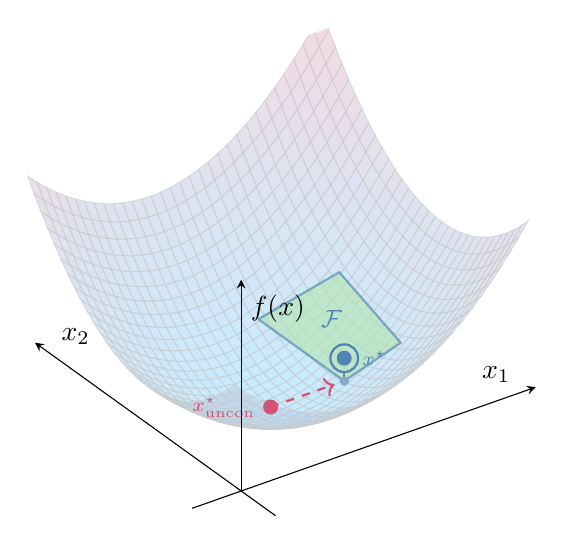
\begin{tikzpicture}
\begin{axis}[
    view={-35}{45},
    width=9cm, height=8cm,
    grid=major,
    xlabel={$x_1$}, ylabel={$x_2$}, zlabel={$f(x)$},
    xmin=-1, xmax=6, ymin=-1, ymax=6, zmin=0, zmax=25,
    axis lines=center,
    axis on top,
    ticks=none,
    colormap={bluepink}{color=(skyblue) color=(deeppink!40)},
]

% 1. 目标函数曲面（抛物面 bowl）
\addplot3[
    surf,
    domain=-0.5:5.5, domain y=-0.5:5.5,
    samples=32,
    opacity=0.55,
    faceted color=black!20,
    z buffer=sort
] {1.2*(x-2)^2 + 1.2*(y-2)^2};

% 2. 底面可行域
\addplot3[
    fill=lightgreen, opacity=0.65, draw=deepblue, thick,
] coordinates {
    (3.5, 4.5, 0)
    (5.5, 5.0, 0)
    (5.0, 2.5, 0)
    (3.5, 2.0, 0)
    (3.5, 4.5, 0)
};
\node[deepblue, font=\small\bfseries] at (axis cs:4.5, 3.8, 0) {$\mathcal{F}$};

% 3. 无约束最优点（碗底）
\addplot3[mark=*, mark size=2.5pt, color=deeppink] coordinates {(2, 2, 0)};
\node[deeppink, left=2pt, font=\scriptsize] at (axis cs:2, 2, 0) {$x^\star_{\text{uncon}}$};

% 4. 约束最优解
\addplot3[mark=*, mark size=2.5pt, color=deepblue] coordinates {(3.5, 2.0, 2.7)};
\addplot3[mark=o, mark size=5pt, color=deepblue, thick] coordinates {(3.5, 2.0, 2.7)};
\node[deepblue, right=3pt, font=\scriptsize\bfseries] at (axis cs:3.5, 2.0, 2.7) {$x^\star$};

% 底面投影点
\addplot3[mark=*, mark size=1.5pt, color=deepblue!70] coordinates {(3.5, 2.0, 0)};

% 5. 辅助线
\addplot3[dashed, thick, gray] coordinates {(3.5, 2.0, 0) (3.5, 2.0, 2.7)};
\addplot3[->, dashed, thick, deeppink] coordinates {(2, 2, 0) (3.3, 2.0, 0)};

\end{axis}
\end{tikzpicture}
}
  \caption{三维曲面视角下的抛物面碗型直觉}
  \label{fig:qp_geometry:3d}
\end{subfigure}
\caption{凸二次规划的几何解释}
\caption*{\scriptsize 左：正定二次型等值线为同心椭圆，线性约束构成凸多边形可行域$\mathcal{F}$，最优解$x^\star$处椭圆与约束边界相切，即KKT 互补松弛。\\右：目标函数在 $x_1,x_2,f$ 空间是开口向上的抛物面，碗底为无约束最优点 $x^\star_{\text{uncon}}$；当该点落在 $\mathcal{F}$ 之外时，最优解 $x^\star$ 落在 $\mathcal{F}$ 内最接近碗底、曲面高度最低的位置。}
\label{fig:qp_geometry}
\end{figure}

\subsection{二次规划}

二次规划（Quadratic Programming, QP）是凸优化的一个重要子类，其目标函数为二次形式，约束条件为线性。标准形式为
\begin{equation}
\begin{aligned}
\min_{\mathbf{x}} \quad & \frac{1}{2}\mathbf{x}^T H \mathbf{x} + \mathbf{f}^T \mathbf{x} \\
\text{s.t.} \quad & A_{eq}\mathbf{x} = \mathbf{b}_{eq} \\
& A_{ineq}\mathbf{x} \leq \mathbf{b}_{ineq} \\
& \mathbf{x}_{lb} \leq \mathbf{x} \leq \mathbf{x}_{ub}
\end{aligned}
\label{eq:qp_standard}
\end{equation}
其中$H$为半正定矩阵$H \succeq 0$，$\mathbf{f}$为线性项系数，$A_{eq}$和$A_{ineq}$分别为等式和不等式约束矩阵。

Apollo Planning模块使用算子分裂二次规划求解器（Operator Splitting Quadratic Program, OSQP）\cite{stellato2020osqp}作为QP求解器。OSQP基于交替方向乘子法（Alternating Direction Method of Multipliers, ADMM），具有以下优点。
\begin{enumerate}
\item 支持稀疏矩阵运算，适合大规模问题；
\item 可处理不可行问题，返回近似解；
\item 无需活跃集策略，对初始点不敏感；
\item 计算复杂度为$O(n^2)$至$O(n^3)$，满足实时性要求。
\end{enumerate}

\subsection{路径规划中的QP建模}

在Apollo的路径规划中，轨迹被表示为关于参数$t$的分段多项式。以五次多项式为例，第$i$段样条的形式为
\begin{equation}
f_i(t) = a_{i,0} + a_{i,1}t + a_{i,2}t^2 + a_{i,3}t^3 + a_{i,4}t^4 + a_{i,5}t^5
\label{eq:quintic_poly}
\end{equation}

规划问题的目标函数通常包含以下代价项
\begin{equation}
J = \underbrace{w_1 \int (l'')^2 ds}_{\text{曲率平滑}} + \underbrace{w_2 \int (l''')^2 ds}_{\text{曲率变化率}} + \underbrace{w_3 \sum_j \| l(s_j) - l_{ref,j} \|^2}_{\text{参考线跟踪}}
\label{eq:path_cost}
\end{equation}
其中$w_1, w_2, w_3$为各项权重，$l''$和$l'''$分别为横向偏移的二阶和三阶导数，$l_{ref,j}$为参考线对应的横向偏移。约束条件包括初始状态约束、样条节点连续性约束$C^2$或$C^3$、路径边界约束等。

上述五次多项式表示是Apollo早期版本中使用的路径参数化方式。在当前Apollo版本中，主流的\texttt{PiecewiseJerkPathOptimizer}采用离散化表示方法，直接以纵向采样点的横向偏移$l_i$作为优化变量，利用有限差分近似一阶和二阶导数，从而将路径优化转化为标准二次规划问题。本文后续章节的分析基于该离散化实现方式。

\section{SL图与路径边界}

在Frenet坐标系下，路径规划的核心任务是确定自车在每个纵向位置$s$处的横向偏移$l(s)$。为此，需要在纵向位置-横向偏移（Station-Lateral, SL）空间，即由纵向位置$s$与横向偏移$l$构成的二维平面中，构建路径的可通行边界。

\subsection{障碍物的SL投影}

每个障碍物在SL空间中占据一个区域。设第$i$个障碍物的SL投影为矩形
\begin{equation}
O_i = [s_i^{min}, s_i^{max}] \times [l_i^{min}, l_i^{max}]
\end{equation}
其中$[s_i^{min}, s_i^{max}]$为障碍物沿参考线的纵向投影范围，$[l_i^{min}, l_i^{max}]$为其横向占据范围。图\ref{fig:sl_projection}展示了障碍物从笛卡尔空间到SL空间的投影过程。

\begin{figure}[htbp]
\centering
\begin{subfigure}[b]{0.48\textwidth}
  \centering
  \adjustbox{max width=\textwidth}{% SL空间障碍物投影示意图（S弯道场景）— 子图 a：笛卡尔空间
\begin{tikzpicture}[scale=0.9, transform shape]

  % 道路背景（参考线 ±1.2 的条带，与子图 b 一致）
  \begin{scope}[on background layer]
    \fill[bglight]
      plot[domain=0:7, samples=100] (\x, {1.5*sin(\x*50)+1.2})
      -- plot[domain=7:0, samples=100] (\x, {1.5*sin(\x*50)-1.2})
      -- cycle;
  \end{scope}

  % S型参考线（正弦函数）
  \draw[deepblue, very thick]
    plot[domain=0:7, samples=100] (\x, {1.5*sin(\x*50)});
  \node[deepblue, font=\footnotesize, right] at (7.1,{1.5*sin(350)}) {参考线};

  % 道路边界（参考线 ±1.2 偏移）
  \draw[gray, thick, dashed]
    plot[domain=0:7, samples=100] (\x, {1.5*sin(\x*50)+1.2});
  \draw[gray, thick, dashed]
    plot[domain=0:7, samples=100] (\x, {1.5*sin(\x*50)-1.2});

  % 障碍物 O1（s≈1.5 处，参考线上方偏）
  \pgfmathsetmacro{\oa}{1.5*sin(1.5*50)}
  \pgfmathsetmacro{\oaAngle}{atan(1.5*50*cos(1.5*50)*3.14159/180)}
  \fill[dangerred!40, draw=dangerred, thick, rounded corners=1pt,
        rotate around={\oaAngle:(1.5,\oa+0.5)}]
    (1.1,\oa+0.2) rectangle (1.9,\oa+0.8);
  \node[font=\small\bfseries] at (1.5,\oa+0.5) {$O_1$};

  % 障碍物 O2（s≈3.5 处，弯顶附近）
  \pgfmathsetmacro{\ob}{1.5*sin(3.5*50)}
  \pgfmathsetmacro{\obAngle}{atan(1.5*50*cos(3.5*50)*3.14159/180)}
  \fill[dangerred!40, draw=dangerred, thick, rounded corners=1pt,
        rotate around={\obAngle:(3.5,\ob-0.4)}]
    (3.1,\ob-0.7) rectangle (3.9,\ob-0.1);
  \node[font=\small\bfseries] at (3.5,\ob-0.4) {$O_2$};

  % 障碍物 O3（s≈5.8 处，弯道后段）
  \pgfmathsetmacro{\oc}{1.5*sin(5.8*50)}
  \pgfmathsetmacro{\ocAngle}{atan(1.5*50*cos(5.8*50)*3.14159/180)}
  \fill[dangerred!40, draw=dangerred, thick, rounded corners=1pt,
        rotate around={\ocAngle:(5.8,\oc+0.4)}]
    (5.4,\oc+0.1) rectangle (6.2,\oc+0.7);
  \node[font=\small\bfseries] at (5.8,\oc+0.4) {$O_3$};

  % 自车（沿参考线切线方向贴合，风格与障碍物一致但色调为蓝）
  \pgfmathsetmacro{\egoX}{0.5}
  \pgfmathsetmacro{\egoY}{1.5*sin(\egoX*50)}
  \pgfmathsetmacro{\egoAngle}{atan(1.309*cos(\egoX*50))}
  \fill[deepblue!25, draw=deepblue, thick, rounded corners=1pt,
        rotate around={\egoAngle:(\egoX,\egoY)}]
    ({\egoX-0.32},{\egoY-0.18}) rectangle ({\egoX+0.32},{\egoY+0.18});
  \fill[deepblue,
        rotate around={\egoAngle:(\egoX,\egoY)}]
    ({\egoX+0.32},{\egoY-0.12}) -- ({\egoX+0.50},{\egoY}) -- ({\egoX+0.32},{\egoY+0.12}) -- cycle;
  \node[deepblue, font=\scriptsize] at (1.4,-0.3) {自车};
  \draw[deepblue, thin] (1.15,-0.25) -- ({\egoX+0.15},{\egoY-0.35});

  % 坐标轴
  \draw[-{Stealth}, thick, gray] (-0.3,-2.5) -- (1.5,-2.5) node[right, font=\footnotesize] {$x$};
  \draw[-{Stealth}, thick, gray] (-0.3,-2.5) -- (-0.3,-1.2) node[above, font=\footnotesize] {$y$};

\end{tikzpicture}
}
  \caption{笛卡尔空间中的S弯道场景}
\end{subfigure}
\hfill
\begin{subfigure}[b]{0.48\textwidth}
  \centering
  \adjustbox{max width=\textwidth}{% SL空间障碍物投影示意图 — 子图 b：SL空间
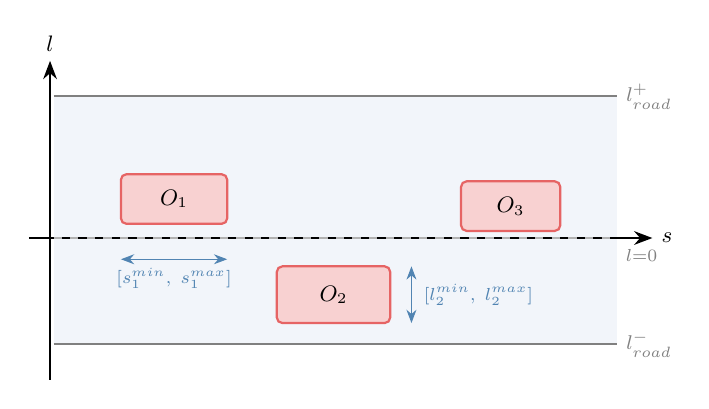
\begin{tikzpicture}[scale=0.9, transform shape]

  % 坐标轴（先画，不被遮挡）
  \draw[-{Stealth}, thick] (-0.3,0) -- (8.5,0) node[right, font=\small\bfseries] {$s$};
  \draw[-{Stealth}, thick] (0,-2.0) -- (0,2.5) node[above, font=\small\bfseries] {$l$};

  % 道路背景（在坐标轴之后，用 scope + opacity 避免遮挡）
  \begin{scope}[on background layer]
    \fill[bglight] (0.05,-1.5) rectangle (8.0,2.0);
  \end{scope}

  % 道路边界
  \draw[gray, thick] (0.05,2.0) -- (8.0,2.0) node[right, font=\footnotesize] {$l_{road}^+$};
  \draw[gray, thick] (0.05,-1.5) -- (8.0,-1.5) node[right, font=\footnotesize] {$l_{road}^-$};

  % 参考线
  \draw[dashed, gray!60] (0.05,0) -- (8.0,0);
  \node[gray, font=\scriptsize, right] at (8.0,-0.25) {$l{=}0$};

  % O1 SL矩形（弯道前段，l > 0）
  \fill[dangerred!30, draw=dangerred, thick, rounded corners=2pt]
    (1.0,0.2) rectangle (2.5,0.9);
  \node[font=\small\bfseries] at (1.75,0.55) {$O_1$};
  \draw[{Stealth}-{Stealth}, thin, deepblue] (1.0,-0.3) -- (2.5,-0.3);
  \node[deepblue, font=\scriptsize, below] at (1.75,-0.3) {$[s_1^{min},\;s_1^{max}]$};

  % O2 SL矩形（弯道中段，l < 0）
  \fill[dangerred!30, draw=dangerred, thick, rounded corners=2pt]
    (3.2,-1.2) rectangle (4.8,-0.4);
  \node[font=\small\bfseries] at (4.0,-0.8) {$O_2$};
  \draw[{Stealth}-{Stealth}, thin, deepblue] (5.1,-1.2) -- (5.1,-0.4);
  \node[deepblue, font=\scriptsize, right] at (5.15,-0.8) {$[l_2^{min},\;l_2^{max}]$};

  % O3 SL矩形（弯道后段，l > 0）
  \fill[dangerred!30, draw=dangerred, thick, rounded corners=2pt]
    (5.8,0.1) rectangle (7.2,0.8);
  \node[font=\small\bfseries] at (6.5,0.45) {$O_3$};

\end{tikzpicture}
}
  \caption{对应的SL空间投影}
\end{subfigure}
\caption{SL空间中障碍物投影示意图}
\caption*{\scriptsize 弯道上各障碍物沿参考线投影后，在SL空间中均表示为轴对齐矩形$[s_i^{min},s_i^{max}] \times [l_i^{min},l_i^{max}]$。}
\label{fig:sl_projection}
\end{figure}

\subsection{路径边界构建}

路径规划需要在SL空间中找到一条横向轨迹$l(s)$，使其不与任何障碍物碰撞。这要求在每个$s$处确定横向可通行区间$[l^-(s), l^+(s)]$，其中$l^+(s)$为上界即左侧限制，$l^-(s)$为下界即右侧限制。

对于每个在位置$s$处活跃的障碍物$O_i$，即满足$s \in [s_i^{min}, s_i^{max}]$的障碍物，规划系统需要做出避让方向决策$d_i \in \{L, R\}$，若选择右绕，即$d_i = R$，则障碍物约束路径上界$l^+(s) \leq l_i^{min} - \delta$；若选择左绕，即$d_i = L$，则约束下界$l^-(s) \geq l_i^{max} + \delta$。其中$\delta$为安全裕度。

图\ref{fig:nudge_decision}直观展示了两种避让方向决策对路径边界的影响。图\ref{fig:nudge_decision:a}为右绕情形，障碍物位于车道中线上方，决策$d_i=R$使得原本位于车道左侧边界的上界被压低至$u_i=l_i^{min}-\delta$，自车须在该上界之下寻找路径。图\ref{fig:nudge_decision:b}为左绕情形，障碍物位于车道中线下方，决策$d_i=L$使得原本位于车道右侧边界的下界被抬高至$v_i=l_i^{max}+\delta$。任一次避让决策都是对路径可行空间的单边收紧，是后续章节理解独立决策导致矛盾避让问题的直接几何基础。

\begin{figure}[htbp]
\centering
\begin{subfigure}[b]{0.48\textwidth}
  \centering
  \adjustbox{max width=\linewidth}{\input{../图片/fig_nudge_decision_a}}
  \caption{RIGHT\_NUDGE}
  \label{fig:nudge_decision:a}
\end{subfigure}\hfill
\begin{subfigure}[b]{0.48\textwidth}
  \centering
  \adjustbox{max width=\linewidth}{% LEFT_NUDGE 决策对边界影响（子图 b）
% 障碍物在参考线下方，左绕 → 下界被抬高至 v_i = l_i^max + δ
\begin{tikzpicture}[scale=1.0, transform shape]

  % 道路背景
  \fill[bglight] (0,-2.5) rectangle (7.5,2.5);

  % 道路边界
  \draw[gray, thick] (0, 2.5) -- (7.5, 2.5);
  \node[gray, font=\scriptsize, above left] at (7.5, 2.5) {$l_{road}^+$};
  \draw[gray, thick] (0,-2.5) -- (7.5,-2.5);
  \node[gray, font=\scriptsize, below left] at (7.5,-2.5) {$l_{road}^-$};

  % 参考线
  \draw[gray, dashed] (0,0) -- (7.5,0);
  \node[gray, font=\scriptsize, right] at (7.5,0) {$l{=}0$};

  % l 轴
  \draw[-{Stealth}, thick] (0.3,-2.5) -- (0.3,2.8) node[above, font=\footnotesize] {$l$};

  % 障碍物 O_i（参考线下方）
  \fill[dangerred!70, draw=dangerred, thick] (2.5,-1.5) rectangle (4.5,-0.5);
  \node[white, font=\footnotesize\bfseries] at (3.5,-1.0) {$O_i$};

  % 障碍物膨胀虚线框
  \draw[dangerred!70, dashed, thick] (2.2,-1.9) rectangle (4.8,-0.1);
  \node[dangerred!70, font=\scriptsize, right] at (4.9,-1.5) {$+\delta$};

  % 下界 l-(s)：从道路下界 → 抬高到 v_i → 恢复道路下界
  % 与道路边界连起来
  \draw[deepblue, very thick]
    (0,-2.5) -- (2.2,-2.5) -- (2.2,-0.1) -- (4.8,-0.1) -- (4.8,-2.5) -- (7.5,-2.5);
  \node[deepblue, font=\small] at (3.5,0.3) {$l^-(s) = v_i$};

  % 上界 l+(s)：保持道路上界不变
  \draw[deeppink, very thick, dashed]
    (0, 2.5) -- (7.5, 2.5);
  \node[deeppink, font=\small, below left] at (7.5, 2.3) {$l^+(s)$};

  % v_i 标注
  \draw[{Stealth}-{Stealth}, thin, deepblue] (5.2,-2.5) -- (5.2,-0.1);
  \node[deepblue, font=\scriptsize, right] at (5.3,-1.3) {被压缩};

  % 自车轨迹：起点终点在 l=0，向上远离障碍物弯曲
  \draw[deepblue, very thick, -{Stealth}]
    plot[smooth, tension=0.55] coordinates
      {(0.5, 0) (1.5, 0.3) (2.5, 0.8) (3.5, 1.0) (4.5, 0.8) (5.5, 0.3) (6.5, 0)};
  \node[deepblue, font=\footnotesize\bfseries, above] at (3.5,1.2) {自车轨迹};

\end{tikzpicture}
}
  \caption{LEFT\_NUDGE}
  \label{fig:nudge_decision:b}
\end{subfigure}
\caption{避让方向决策对路径边界的影响}
\label{fig:nudge_decision}
\end{figure}

当多个障碍物同时活跃时，所有约束取交集。路径可行的条件是$l^+(s) \geq l^-(s) + W_{ego}$，其中$W_{ego}$为自车宽度。若该条件不满足，路径被判定为阻塞，即BLOCKED。

避让方向的选择本质上是一个组合优化问题，$n$个障碍物各有两种选择，共$2^n$种组合。如何高效地找到使通行带最宽的决策组合，是本文第\ref{chap:group}章的核心研究内容。

\section{ST图与速度规划基础}

SL图负责描述路径的几何可行性，而纵向位移-时间（Station-Time, ST）图则描述路径已定情况下的速度可行性。ST图的横轴为时间$t$，纵轴为沿参考线的累积弧长$s$，自车运动被描绘为一条在$s$随$t$单调递增的曲线，斜率即瞬时速度$\dot{s}$。

\subsection{ST图中的障碍物与速度约束}

障碍物在ST图中的表示取决于其运动状态。静态障碍物在参考线上的投影长度固定，在ST图中表现为一个沿时间轴方向延伸的平行带状矩形区域。动态障碍物的位置随时间改变，在ST图中通常表现为一个倾斜的平行四边形，其斜率由障碍物沿参考线方向的速度决定。

图\ref{fig:st_graph}展示了ST图的基本原理以及两种典型的速度决策方式。当障碍物占据了ST平面中的禁行区域，即图中红色与橙色矩形或平行四边形，自车轨迹必须绕过这些区域。若轨迹位于障碍物的下方，即$s$值较小的一侧，则称为避让即YIELD决策，自车减速让行；若轨迹位于障碍物的上方，即$s$值较大的一侧，则称为超越即OVERTAKE决策，自车加速通过。两种决策对应完全不同的速度曲线，且各自具有不同的可行条件和安全边际。

\begin{figure}[htbp]
\centering
\adjustbox{max width=0.8\textwidth}{% ST图原理示意图
\begin{tikzpicture}[scale=0.85, transform shape]
  % 坐标轴
  \draw[-Stealth, thick] (0,0) -- (9,0) node[right, font=\small\bfseries] {$t$ (s)};
  \draw[-Stealth, thick] (0,0) -- (0,7.5) node[above, font=\small\bfseries] {$s$ (m)};

  % 刻度
  \foreach \t in {1,...,7} {
    \draw (\t, -0.1) -- (\t, 0.1);
    \node[below, font=\footnotesize] at (\t, -0.1) {\t};
  }
  \foreach \s in {1,...,7} {
    \draw (-0.1, \s) -- (0.1, \s);
    \node[left, font=\footnotesize] at (-0.1, \s) {\pgfmathparse{int(\s*5)}\pgfmathresult};
  }

  % 静态障碍物ST边界（矩形）
  \fill[dangerred!30, draw=dangerred, thick] (0,2.5) rectangle (7.5,3.5);
  \node[font=\footnotesize\bfseries, dangerred] at (3.8,3.0) {静态障碍物};

  % 动态障碍物ST边界（倾斜平行四边形）
  \fill[lightorange!60, draw=lightorange!80!black, thick]
    (1,5.5) -- (5,6.5) -- (5,7.2) -- (1,6.2) -- cycle;
  \node[font=\footnotesize\bfseries, lightorange!80!black] at (3,6.6) {动态障碍物};

  % 可行轨迹（绿色曲线 - 从障碍物下方通过）
  \draw[very thick, lightgreen!70!black, -{Stealth}]
    plot[smooth, tension=0.5] coordinates {(0,0.5) (1,1.2) (2,1.8) (3,2.1) (4,2.2) (5,2.3) (6,2.3) (7,2.4)};
  \node[lightgreen!70!black, font=\footnotesize\bfseries] at (7.5,2.7) {轨迹1(YIELD)};

  % 可行轨迹2（蓝色曲线 - 从障碍物上方通过）
  \draw[very thick, deepblue, dashed, -{Stealth}]
    plot[smooth, tension=0.5] coordinates {(0,0.5) (0.8,1.8) (1.5,3.0) (2,4.0) (3,4.8) (4,5.3) (5,5.5) (6,5.8) (7,6.0)};
  \node[deepblue, font=\footnotesize\bfseries] at (7.5,6.3) {轨迹2(OVERTAKE)};

  % 安全距离标注
  \draw[{Stealth}-{Stealth}, thick, deeppink] (7.8, 2.5) -- (7.8, 3.5);
  \node[deeppink, font=\tiny, right] at (7.9, 3.0) {$d_{ext}$};

  % 不可行区域标注
  \draw[-Stealth, thick, gray] (5.5, 4.5) -- (4.5, 3.3);
  \node[gray, font=\footnotesize, right] at (5.2, 4.7) {禁行区域};

  % 图例
  \fill[dangerred!30, draw=dangerred] (0.5,-1.0) rectangle (1.2,-0.6);
  \node[right, font=\footnotesize] at (1.3,-0.8) {静态障碍物ST边界};
  \fill[lightorange!60, draw=lightorange!80!black] (4.5,-1.0) rectangle (5.2,-0.6);
  \node[right, font=\footnotesize] at (5.3,-0.8) {动态障碍物ST边界};
\end{tikzpicture}
}
\caption{ST图原理与YIELD/OVERTAKE决策}
\label{fig:st_graph}
\end{figure}

在此基础上，为保证安全，Apollo对每个障碍物的ST投影额外叠加纵向安全距离$d_s$，使得禁行区沿$s$方向向两侧扩张，得到实际用于约束优化的ST边界。多障碍物情形下所有ST边界取并集，其在每个时刻$t$对应的可行区间的上下界分别构成速度的上下约束曲线$s_{\max}(t)$和$s_{\min}(t)$。两条曲线所围成的区域即为ST走廊，速度优化器在该走廊内寻找平滑、舒适、最快的$s(t)$曲线，构成路径-速度解耦两阶段优化的第二阶段。

\section{Apollo平台架构概述}

\subsection{系统总体架构}

百度Apollo自动驾驶平台\cite{apollo2024}采用模块化设计，主要包含感知、预测、路由、规划和控制五大核心模块。各模块之间通过Cyber RT实时通信框架进行消息传递，采用发布-订阅模式实现松耦合的模块间协作。图\ref{fig:apollo_arch}展示了Apollo平台的总体架构。

\begin{figure}[htbp]
\centering
\adjustbox{max width=0.7\textwidth}{% Apollo平台总体架构图
\begin{tikzpicture}[
    >=Stealth,
    node distance=1.5cm and 2cm,
    sensor/.style={cylinder, shape border rotate=90, aspect=0.25, draw=deepblue, fill=inputyellow, thick, minimum height=1.2cm, minimum width=1.8cm, align=center, font=\small},
    module/.style={rectangle, rounded corners, draw=deepblue, fill=lightblue, thick, minimum width=3cm, minimum height=1.2cm, align=center, font=\small},
    highlight/.style={rectangle, rounded corners, draw=deeppink, fill=improvedpink, thick, minimum width=3cm, minimum height=1.2cm, align=center, font=\small},
    hardware/.style={rectangle, rounded corners, draw=deepblue, fill=lightgreen, thick, minimum width=2cm, minimum height=1cm, align=center, font=\small},
    cyberbox/.style={draw=deepblue, dashed, thick, rounded corners=10pt, inner sep=20pt}
]

% ================= Layer 1: 信息采集 (y=0) =================
\node (lidar)  [sensor] at (0, 0)     {激光雷达\\LiDAR};
\node (camera) [sensor] at (2.4, 0)   {摄像头\\Camera};
\node (radar)  [sensor] at (4.8, 0)   {毫米波雷达\\Radar};
\node (gps)    [sensor] at (8.4, 0)   {GPS / IMU};
\node (hdmap)  [sensor] at (10.8, 0)  {高精地图\\HD Map};

% ================= Layer 2: 环境理解 (y=-2.8) =================
\node (perception)   [module] at (2.4, -2.8)  {感知\\Perception};
\node (localization) [module] at (9.6, -2.8)  {定位\\Localization};

% ================= Layer 3: 意图与路线 (y=-5.2) =================
\node (prediction) [module] at (2.4, -5.2)  {预测\\Prediction};
\node (routing)    [module] at (9.6, -5.2)  {路由\\Routing};

% ================= Layer 4: 核心大脑 (y=-7.6) =================
\node (planning) [highlight] at (6.0, -7.6) {规划\\Planning};

% ================= Layer 5: 动作下达 (y=-9.8) =================
\node (control) [module] at (6.0, -9.8) {控制\\Control};

% ================= Layer 6: 最终执行 (y=-12.0) =================
\node (steering) [hardware] at (3.2, -12.0)  {转向\\Steering};
\node (throttle) [hardware] at (6.0, -12.0)  {油门\\Throttle};
\node (brake)    [hardware] at (8.8, -12.0)  {制动\\Brake};

% ================= Cyber RT =================
\begin{scope}[on background layer]
    \node (cyber) [cyberbox, fit=(perception) (localization) (prediction) (routing) (planning) (control)] {};
    \node [above left, text=deepblue, font=\bfseries] at (cyber.south east) {Cyber RT 通信框架};
\end{scope}

% ================= 数据流向 =================
% 1. 传感器 -> 环境理解
\draw [->, thick] (lidar.south) |- ([yshift=0.5cm]perception.north) -- (perception.north);
\draw [->, thick] (camera.south) -- (perception.north);
\draw [->, thick] (radar.south) |- ([yshift=0.5cm]perception.north) -- (perception.north);
\draw [->, thick] (gps.south) |- ([yshift=0.5cm]localization.north) -- (localization.north);
\draw [->, thick] (hdmap.south) |- ([yshift=0.5cm]localization.north) -- (localization.north);

% HD Map -> Routing
\draw [->, thick, deepblue] (hdmap.east) -- ++(0.5,0) |- (routing.east) node[near end, above, font=\scriptsize, text=black] {全局路网};

% 2. 环境理解 -> 意图与路线
\draw [->, thick] (perception.south) -- (prediction.north);
\draw [->, thick] (perception.south east) -- (routing.north west) node[midway, above right, font=\scriptsize] {规避路况};
\draw [->, thick] (localization.south west) -- (prediction.north east) node[midway, above left, font=\scriptsize] {本车位置};
\draw [->, thick] (localization.south) -- (routing.north);

% 3. 意图与路线 -> 规划
\draw [->, thick] (prediction.south) -- (planning.north west);
\draw [->, thick] (routing.south) -- (planning.north east);

% 4. 规划 -> 控制
\draw [->, thick, deeppink] (planning.south) -- (control.north) node[midway, left, font=\scriptsize, text=black] {轨迹指令};

% 5. 定位 -> 控制
\draw [->, thick, dashed, deepblue!70] (localization.west) -- ++(-0.2,0) |- (control.east) node[near end, above, font=\scriptsize, text=black] {极低延迟位姿};

% 6. 控制 -> 车辆执行
\draw [->, thick] (control.south) -- (throttle.north);
\draw [->, thick] (control.south west) -- (steering.north);
\draw [->, thick] (control.south east) -- (brake.north);

\end{tikzpicture}
}
\caption{Apollo自动驾驶平台总体架构}
\label{fig:apollo_arch}
\end{figure}

\subsection{Cyber RT通信框架}

Cyber RT是Apollo的实时通信框架，替代了早期版本中的机器人操作系统（Robot Operating System, ROS）。相比ROS，Cyber RT具有以下优势。
\begin{enumerate}
\item 更低的消息传递延迟；
\item 确定性的调度机制；
\item 更好的多线程支持；
\item 内置的录制和回放功能。
\end{enumerate}

Planning模块通过Cyber RT订阅以下消息
\begin{itemize}[noitemsep]
\item \texttt{PredictionObstacles}，预测模块输出的障碍物预测轨迹
\item \texttt{Chassis}，底盘状态，含档位、速度、转向
\item \texttt{LocalizationEstimate}，定位信息，含位置、速度、加速度
\item \texttt{TrafficLightDetection}，交通灯检测结果
\item \texttt{PlanningCommand}，规划命令，含路由信息
\end{itemize}

输出消息为\texttt{ADCTrajectory}，包含完整的轨迹点序列及其对应的时间戳、速度、加速度、曲率等信息。

Apollo的路径生成分为宏观与微观两个层次，Planning模块依赖Cyber RT订阅Routing模块输出的全局路由，并在此基础上完成局部轨迹生成。Routing负责宏观路径规划（即确定走哪条路），其基于高精地图的拓扑图以A*算法搜索从起点到终点的全局最优路线，输出道路段序列，仅在目的地变化或需要重路由时触发，属于低频更新。Planning负责微观轨迹规划（即生成具体的局部轨迹），其在Routing提供的参考线基础上结合实时感知与预测信息，以约100ms的周期持续生成局部最优轨迹，是本文研究的重点。

\subsection{Planning模块的Scenario-Stage-Task架构}

Apollo Planning模块采用三级管理架构来实现场景化规划。

\textbf{场景（Scenario）层}\quad{}\texttt{ScenarioManager}根据当前环境状态，如是否有交通灯、停车标志、接近目的地等，选择合适的场景。Apollo支持的场景包括LANE\_FOLLOW、TRAFFIC\_LIGHT\_PROTECTED、STOP\_SIGN\_UNPROTECTED、PULL\_OVER等共19种场景类型，分别对应车道跟随、有保护交通灯、无保护停车标志、靠边停车等驾驶情境。

\textbf{阶段（Stage）层}\quad{}每个Scenario包含一个或多个Stage，表示完成该场景需要经历的不同阶段。例如，停车标志场景可能包含接近停车线、停车等待、通过路口等阶段。

\textbf{任务（Task）层}\quad{}每个Stage包含一个有序的Task列表，Task是最小的规划执行单元。常见的Task包括路径边界决策\texttt{PathBoundsDecider}、路径决策\texttt{PathDecider}、速度边界决策\texttt{SpeedBoundsDecider}、速度优化\texttt{PiecewiseJerkSpeedOptimizer}等。Task按顺序在参考线上依次执行。

这种三级架构使得规划逻辑模块化、可配置，不同场景可以灵活组合不同的Task流水线。

\section{组合优化与区间图基础}

本文第\ref{chap:group}章将多障碍物避让方向选择建模为组合优化问题，并利用区间图的结构性质将指数级搜索空间降至多项式级别。本节介绍相关的数学基础。

\subsection{组合优化概述}

组合优化是在有限或可数无限的离散可行解集合中搜索最优解的数学分支。其一般形式为
\begin{equation}
\mathbf{x}^{*} = \arg\max_{\mathbf{x} \in \mathcal{X}} f(\mathbf{x})
\label{eq:combo_opt}
\end{equation}
其中$\mathcal{X}$为有限可行集，$f$为目标函数。当$\mathcal{X}$由$n$个二值决策变量构成时，可行集的大小为$2^n$，暴力枚举在$n$较大时不可行。

组合优化问题按计算复杂度分为P类和NP-hard类。其中NP为非确定性多项式（Non-deterministic Polynomial, NP）的缩写，NP-hard问题至少与NP类中最难的问题同等困难。P类问题存在多项式时间算法，而NP-hard问题在最坏情况下不存在已知的多项式时间精确算法。然而，许多NP-hard问题在特定的问题结构下可以利用结构性质显著降低求解复杂度。例如，当决策变量之间存在特定的排序或独立性关系时，搜索空间可从指数级降为多项式级。本文第\ref{chap:group}章证明的引理\ref{lem:continuous_partition}正是利用了障碍物在横向排序后最优分割具有连续性这一结构性质，将$2^k$种决策组合降为$k+1$个候选分割点的线性枚举。

\subsection{区间图与连通分量}

在图论中，区间图是一类与实数轴上的区间集合对应的无向图。给定$n$个闭区间$I_1 = [a_1, b_1], I_2 = [a_2, b_2], \ldots, I_n = [a_n, b_n]$，以每个区间为一个顶点，两个顶点之间存在边当且仅当对应区间有交集
\begin{equation}
(I_i, I_j) \in E \iff [a_i, b_i] \cap [a_j, b_j] \neq \emptyset
\label{eq:interval_graph}
\end{equation}

区间图的连通分量可通过扫描线算法在$O(n \log n)$时间内求解。将所有区间按左端点$a_i$升序排列，维护当前连通分量中所有区间右端点的最大值$b_{max}$。依次扫描排序后的区间，若下一个区间的左端点$a_j \leq b_{max}$，则将其并入当前连通分量并更新$b_{max} \leftarrow \max(b_{max}, b_j)$，否则开始新的连通分量。排序需$O(n \log n)$，扫描仅需$O(n)$。

在本文第\ref{chap:group}章中，每个障碍物的纵向占据区间$[s_i^{-}, s_i^{+}]$构成一个区间集合，其区间图的连通分量恰好对应在纵向上彼此关联的障碍物组。不同连通分量的避让决策互不影响，可以独立求解。这一分组机制是本文算法将全局问题分解为多个独立子问题的理论基础。

\subsection{碰撞时间}

碰撞时间（Time-to-Collision, TTC）是交通安全领域衡量碰撞紧迫性的经典指标\cite{paden2016}，定义为在当前运动状态下两个物体发生碰撞所需的时间
\begin{equation}
TTC = \frac{\Delta s}{v_{rel}}
\label{eq:ttc_def}
\end{equation}
其中$\Delta s$为两物体之间的纵向距离，$v_{rel}$为相对接近速度。当$v_{rel} \leq 0$时两物体不在相互接近，$TTC = +\infty$。TTC值越小，碰撞风险越高。

工程上通常按风险等级划分TTC阈值，$TTC < 0.5\,\mathrm{s}$对应紧急制动区间，$0.5\,\mathrm{s} \leq TTC < 1.5\,\mathrm{s}$对应警戒区间，$1.5\,\mathrm{s} \leq TTC < 4\,\mathrm{s}$对应舒适跟车区间。与单纯的距离指标相比，TTC同时编码了距离和速度信息，能更准确地反映碰撞的紧迫程度。

式\eqref{eq:ttc_def}的一维形式假设两物体沿参考线方向共线运动，实际场景中相对运动常具有横向分量。在Frenet坐标系下可将碰撞时间按维度分解，纵向TTC以$\Delta s$与纵向相对速度$\dot{s}_{ego} - \dot{s}_{obs}$构造，横向TTC以$\Delta l$与横向相对速度$\dot{l}_{ego} - \dot{l}_{obs}$构造，二者的较小值反映最先发生碰撞的方向
\begin{equation}
TTC_{2D} = \min\left\{\frac{\Delta s}{\dot{s}_{ego} - \dot{s}_{obs}},\ \frac{\Delta l}{\dot{l}_{ego} - \dot{l}_{obs}}\right\}
\label{eq:ttc_2d}
\end{equation}
该分解形式可直接落到SL投影上，使得TTC可嵌入路径与速度的联合决策，并为第\ref{chap:threat}章多因子威胁度评估提供基础度量。

\section{本章小结}

本章介绍了论文涉及的核心技术与理论基础。Frenet坐标系将二维规划问题分解为纵横向两个一维问题，是Apollo路径规划的坐标基础。凸优化和二次规划为路径优化提供了数学工具，第\ref{chap:group}章的路径边界优化和速度QP融合均建立在该理论之上。SL图中的路径边界构建和障碍物避让方向决策是本文改进的核心对象，第\ref{chap:framework}章将从安全裕度、决策粒度和时空协调三个维度分析其在多障碍物场景下的局限，第\ref{chap:group}章在此基础上建立多障碍物统一规划的数学框架并提出高效求解算法。ST图与速度规划基础为理解路径-速度解耦架构中的协调缺失提供了必要背景，第\ref{chap:st_corridor}章提出的时空可通行走廊即是将时变通行带投影至ST空间、与速度约束融合的机制。组合优化、区间图连通分量和碰撞时间等概念为第\ref{chap:group}章的问题建模、障碍物分组算法和威胁度评估提供了直接的理论支撑。Apollo平台的Scenario-Stage-Task架构为改进算法的集成提供了框架基础。

\chapter{Apollo Planning模块深度分析}
\label{chap:apollo_planning}

本章以Apollo 11.0源码为对象，梳理Planning模块的核心组件及其相互关系，内容包括模块总体架构、\texttt{ReferenceLine}平滑、路径-速度解耦两阶段优化、\texttt{PathBoundsDecider}相关的横向边界构建、\texttt{PathDecider}决策逻辑以及\texttt{SpeedBoundsDecider}的ST边界构建。源码层面的梳理为第\ref{chap:framework}章的问题识别提供事实依据。

\section{Planning模块总体架构}

\subsection{模块入口与数据流}

Planning模块的主入口函数为\texttt{PlanningComponent::Proc()}，每个规划周期由Cyber RT调度执行。从输入消息到输出轨迹的完整数据流如图\ref{fig:planning_flow}所示。整个处理过程划分为三个层次的函数调用。最外层的\texttt{PlanningComponent::Proc()}负责从Cyber RT消息通道读取五类输入数据并完成路由检查和有效性校验。中间层的\texttt{OnLanePlanning::RunOnce()}完成车辆状态更新、参考线缓存读取、轨迹拼接和Frame初始化等准备工作。参考线的生成与平滑并不在RunOnce的调用栈内，而是由\texttt{ReferenceLineProvider}托管的独立异步线程\texttt{GenerateThread}以50\,ms周期持续执行，RunOnce仅通过\texttt{GetReferenceLines()}读取其最新缓存，并通过\texttt{UpdateVehicleState()}和\texttt{UpdatePlanningCommand()}向该线程注入触发输入。核心执行层的\texttt{OnLanePlanning::Plan()}通过\texttt{ScenarioManager}选择场景，再由Stage驱动Task列表按顺序执行，最终产生\texttt{ADCTrajectory}轨迹输出。

\begin{figure}[htbp]
\centering
\adjustbox{max width=\textwidth}{% Planning 模块单周期数据流
\begin{tikzpicture}[
    scale=0.85, transform shape,
    >=Stealth,
    % 输入小盒
    inp/.style={rectangle, rounded corners=1pt, draw=deepblue,
                fill=inputyellow, minimum width=1.65cm, minimum height=0.6cm,
                font=\footnotesize, align=center, inner sep=2pt},
    % 层内子步骤
    step box/.style={rectangle, rounded corners=2pt, draw=deepblue,
                     fill=lightblue, minimum width=1.8cm, minimum height=0.6cm,
                     font=\footnotesize, align=center, inner sep=2pt},
    % 改进层子步骤
    step imp/.style={rectangle, rounded corners=2pt, draw=deeppink,
                     fill=improvedpink, minimum width=1.8cm, minimum height=0.6cm,
                     font=\footnotesize, align=center, inner sep=2pt},
    % 层背景
    layer bg/.style={rectangle, rounded corners=6pt, fill=bglight,
                     draw=deepblue!50, inner sep=8pt},
    % 改进层背景
    layer imp/.style={rectangle, rounded corners=6pt, fill=improvedpink!15,
                      draw=deeppink!60, inner sep=8pt},
    % 输出节点
    out box/.style={rectangle, rounded corners=3pt, draw=deeppink,
                    fill=outputpink, minimum width=4cm, minimum height=0.7cm,
                    font=\small\bfseries, align=center},
]

% ===================== 输入层 (y = 0) =====================
\node[inp] (i1) at (-4,   0) {Prediction\\[-1pt]Obstacles};
\node[inp] (i2) at (-2,   0) {Chassis};
\node[inp] (i3) at ( 0,   0) {Localization};
\node[inp] (i4) at ( 2,   0) {TrafficLight};
\node[inp] (i5) at ( 4,   0) {Planning\\[-1pt]Command};
\node[font=\small, text=deepblue, anchor=east] at (-5.2, 0) {Cyber RT 输入};

% 汇聚点
\coordinate (merge) at (0, -1.0);
\foreach \i in {i1,i2,i3,i4,i5}{
    \draw[flow] (\i.south) -- (merge);
}

% ===================== Layer 1: Proc() (y = -2.2) =====================
\node[step box] (p1) at (-2.8, -2.2) {CheckRerouting};
\node[step box] (p2) at ( 0,   -2.2) {构建 LocalView};
\node[step box] (p3) at ( 2.8, -2.2) {CheckInput};

\draw[flow] (p1) -- (p2);
\draw[flow] (p2) -- (p3);

% 隐藏锚点，使三层 fit 宽度一致
\coordinate (L1pad-l) at (-4.4, -2.2);
\coordinate (L1pad-r) at ( 4.4, -2.2);

\begin{scope}[on background layer]
    \node[layer bg, fit=(L1pad-l)(L1pad-r)(p1)(p2)(p3),
          label={[font=\small, text=deepblue, anchor=east]left:Proc()}] (L1) {};
\end{scope}

\draw[flow, line width=1.2pt] (merge) -- (L1.north);

% ===================== Layer 2: RunOnce() (y = -4.2) =====================
\node[step box] (r1) at (-3.4, -4.2) {VehicleState\\[-1pt]更新};
\node[step box] (r2) at (-1.1, -4.2) {参考线平滑};
\node[step box] (r3) at ( 1.2, -4.2) {轨迹拼接};
\node[step box] (r4) at ( 3.4, -4.2) {Frame\\[-1pt]初始化};

\draw[flow] (r1) -- (r2);
\draw[flow] (r2) -- (r3);
\draw[flow] (r3) -- (r4);

\begin{scope}[on background layer]
    \node[layer bg, fit=(r1)(r2)(r3)(r4),
          label={[font=\small, text=deepblue, anchor=east]left:RunOnce()}] (L2) {};
\end{scope}

\draw[flow, line width=1.2pt] (L1.south) -- (L2.north);

% ===================== Layer 3: Plan() (y = -6.2) =====================
\node[step imp] (s1) at (-3.4, -6.2) {Scenario\\[-1pt]Manager};
\node[step imp] (s2) at (-1.1, -6.2) {Scenario\\[-1pt]::Process};
\node[step imp] (s3) at ( 1.2, -6.2) {Stage\\[-1pt]::Process};
\node[step imp] (s4) at ( 3.4, -6.2) {Task\\[-1pt]::Execute};

\draw[flowimp] (s1) -- (s2);
\draw[flowimp] (s2) -- (s3);
\draw[flowimp] (s3) -- (s4);

\begin{scope}[on background layer]
    \node[layer imp, fit=(s1)(s2)(s3)(s4),
          label={[font=\small, text=deeppink, anchor=east]left:Plan()}] (L3) {};
\end{scope}

\node[font=\footnotesize, text=deeppink!80!black, anchor=west] at (L3.east) {~~核心执行层};

\draw[flowimp, line width=1.2pt] (L2.south) -- (L3.north);

% ===================== 输出 (y = -8.0) =====================
\node[out box] (output) at (0, -8.0) {ADCTrajectory};

\draw[flowimp, line width=1.2pt] (L3.south) -- (output.north);

\end{tikzpicture}
}
\caption{Planning模块数据流}
\label{fig:planning_flow}
\end{figure}

Task列表内部不进行回溯迭代，各Task按配置顺序单向执行，前序Task的输出作为后续Task的输入。这种流水线式的结构对每个Task的正确性要求较高。若前序Task中由\texttt{PathBoundsDeciderUtil}承载的路径边界构建逻辑出现不必要的保守决策，后续Task无法修正，只能在其输出之上继续处理。这一特征决定了横向边界的构造方式对最终轨迹的影响难以在下游环节被弥补。

\subsection{DependencyInjector依赖注入}

Apollo通过\texttt{DependencyInjector}类实现依赖注入，在\texttt{PlanningComponent::Init()}中创建并传递给各组件。表\ref{tab:dependency_injector}列出了其注入的主要依赖，包括规划上下文、历史轨迹和车辆状态等共享信息。

\begin{table}[htbp]
\centering
\caption{DependencyInjector注入的依赖组件}
\label{tab:dependency_injector}
\begin{tabular}{ll}
\toprule
依赖组件 & \textbf{功能说明} \\
\midrule
PlanningContext & 规划上下文，存储跨周期状态信息 \\
FrameHistory & Frame历史记录，用于轨迹拼接和平滑 \\
History & \texttt{ADCTrajectory}历史记录 \\
EgoInfo & 自车信息，含前方障碍物距离与路由信息 \\
VehicleStateProvider & 车辆状态，含位置、速度、加速度与航向 \\
LearningBasedData & 学习模型数据，供强化学习模式使用 \\
\bottomrule
\end{tabular}
\end{table}

\subsection{场景管理机制}

\texttt{ScenarioManager}在每个规划周期检查当前环境状态，通过调用各Scenario的\texttt{IsTransferable()}方法判断是否需要切换场景。图\ref{fig:scenario_hierarchy}展示了Scenario-Stage-Task的三级层次结构。Apollo支持19种场景类型，表\ref{tab:scenarios}列出了主要场景及其触发条件。

\begin{figure}[htbp]
\centering
\adjustbox{max width=\textwidth}{% Scenario-Stage-Task层次结构图
\begin{tikzpicture}[
    scale=0.85, transform shape,
    level 1/.style={sibling distance=5.5cm, level distance=2cm},
    level 2/.style={sibling distance=3cm, level distance=2cm},
    level 3/.style={sibling distance=2.2cm, level distance=2cm},
    scenar/.style={rectangle, draw=deepblue, fill=deepblue!60, text=white, font=\small\bfseries, rounded corners, minimum width=2.5cm, minimum height=0.8cm, align=center},
    stag/.style={rectangle, draw=deepblue, fill=skyblue, font=\small, rounded corners, minimum width=2.2cm, minimum height=0.8cm, align=center},
    tas/.style={rectangle, draw=deepblue, fill=lightblue, font=\footnotesize, rounded corners, minimum width=1.8cm, minimum height=0.7cm, align=center},
    mgr/.style={rectangle, draw=deeppink, fill=improvedpink, font=\small\bfseries, rounded corners, minimum width=3.5cm, minimum height=0.9cm, align=center}
]

  % ScenarioManager
  \node[mgr] (mgr) at (0, 1.5) {ScenarioManager};

  % Scenarios
  \node[scenar] (lf) at (-4, -0.5) {LANE\_FOLLOW};
  \node[scenar] (tl) at (0, -0.5) {TRAFFIC\_LIGHT\\PROTECTED};
  \node[scenar] (ss) at (4, -0.5) {STOP\_SIGN\\UNPROTECTED};
  \node[font=\small, gray] at (7, -0.5) {$\cdots$（共19种）};

  % Stages for LANE_FOLLOW
  \node[stag] (stage1) at (-4, -2.5) {LaneFollow\\Stage};

  % Tasks
  \node[tas] (t1) at (-7.8, -4.5) {LaneFollow\\Path};
  \node[tas] (t2) at (-5.3, -4.5) {Path\\Decider};
  \node[tas] (t3) at (-2.8, -4.5) {SpeedBounds\\Decider};
  \node[tas] (t4) at (-0.3, -4.5) {PiecewiseJerk\\Speed};
  \node[font=\footnotesize, gray] at (1.6, -4.5) {$\cdots$};

  % Stages for STOP_SIGN
  \node[stag] (ss1) at (3, -2.5) {Approach};
  \node[stag] (ss2) at (5.5, -2.5) {Creep};

  % 连线
  \draw[-Stealth, thick, deeppink] (mgr) -- (lf);
  \draw[-Stealth, thick, deeppink] (mgr) -- (tl);
  \draw[-Stealth, thick, deeppink] (mgr) -- (ss);

  \draw[-Stealth, thick, deepblue] (lf) -- (stage1);
  \draw[-Stealth, thick, deepblue] (ss) -- (ss1);
  \draw[-Stealth, thick, deepblue] (ss) -- (ss2);

  \draw[-Stealth, thick, deepblue!60] (stage1) -- (t1);
  \draw[-Stealth, thick, deepblue!60] (stage1) -- (t2);
  \draw[-Stealth, thick, deepblue!60] (stage1) -- (t3);
  \draw[-Stealth, thick, deepblue!60] (stage1) -- (t4);

  % 层次标注
  \node[font=\small\bfseries, deepblue, rotate=90] at (-9.8, -0.5) {Scenario层};
  \node[font=\small\bfseries, deepblue, rotate=90] at (-9.8, -2.5) {Stage层};
  \node[font=\small\bfseries, deepblue, rotate=90] at (-9.8, -4.5) {Task层};

  % 虚线分隔
  \draw[dashed, gray] (-9.3, -1.5) -- (7.5, -1.5);
  \draw[dashed, gray] (-9.3, -3.5) -- (7.5, -3.5);
\end{tikzpicture}
}
\caption{Scenario-Stage-Task三级管理架构}
\label{fig:scenario_hierarchy}
\end{figure}

图\ref{fig:planning_arch}以LaneFollow场景的默认流水线配置为基准，展开了Stage内部\texttt{task\_list\_}的真实执行顺序。路径侧由四个互斥的路径生成Task即\texttt{LaneChangePath}、\texttt{LaneFollowPath}、\texttt{LaneBorrowPath}、\texttt{FallbackPath}择一执行，再串接\texttt{PathDecider}与\texttt{RuleBasedStopDecider}；速度侧依次为\texttt{SpeedBoundsDecider}（PRIORI）、\texttt{PathTimeHeuristicOptimizer}、\texttt{SpeedDecider}、\texttt{SpeedBoundsDecider}（FINAL）和\texttt{PiecewiseJerkSpeedOptimizer}，其中\texttt{SpeedBoundsDecider}在管线中出现两次。历史版本中作为独立Task的\texttt{PathBoundsDecider}在Apollo 11.0中主要表现为工具类\texttt{PathBoundsDeciderUtil}，被上述四个路径生成Task内部共同调用以构建横向边界$[l^{-}(s), l^{+}(s)]$，本文改进点即定位于该边界构建逻辑，图中以星标与粉色高亮标识。外部输入侧，\texttt{ReferenceLineProvider}在独立异步线程中以50\,ms周期持续生成参考线，\texttt{TrajectoryStitcher}基于前一帧轨迹完成时间拼接，二者共同馈入Stage的输入端；最终由\texttt{ReferenceLineInfo::CombinePathAndSpeedProfile}将路径与速度合成为\texttt{ADCTrajectory}输出。

\begin{figure}[htbp]
\centering
\adjustbox{max width=\textwidth}{% Planning模块总体架构图
\begin{tikzpicture}[
    node distance=0.9cm,
    scale=1.0, transform shape,
    manager/.style={rectangle, draw=deepblue, minimum width=3.5cm, minimum height=1.2cm, fill=deepblue!60, font=\normalsize\bfseries, align=center, text width=3.3cm, text=white},
    task/.style={rectangle, draw=deepblue, minimum width=3.8cm, minimum height=1.2cm, fill=lightblue, font=\normalsize, align=center, text width=3.6cm},
    improved/.style={rectangle, draw=deeppink, minimum width=3.8cm, minimum height=1.2cm, fill=improvedpink, font=\normalsize, align=center, text width=3.6cm},
    final/.style={rectangle, draw=deepblue, minimum width=5cm, minimum height=1.2cm, fill=outputpink, font=\normalsize\bfseries, align=center, text width=4.8cm},
    arrow/.style={thick, -Stealth, deepblue}
]

% 标题
\node[font=\Large\bfseries] (title) at (0, 2) {Planning 模块总体架构};

% 管理层
\node[manager] (scenario) at (-5.2, 0) {Scenario\\Manager};
\node[manager] (stage) at (0, 0) {Stage\\Manager};
\node[manager] (task_runner) at (5.2, 0) {Task\\Runner};

% 管理层标签
\node[font=\small, below=0.15cm of scenario] {场景识别切换};
\node[font=\small, below=0.15cm of stage] {阶段状态管理};
\node[font=\small, below=0.15cm of task_runner] {任务执行调度};

% 箭头 - 管理层
\draw[arrow] (scenario) -- (stage);
\draw[arrow] (stage) -- (task_runner);

% 分隔线
\draw[thick, dashed, deepblue] (-8, -2) -- (8, -2);
\node[font=\large\bfseries, color=deepblue] at (0, -2.5) {核心Task模块};

% 左列 - 路径相关
\node[task] (ref_provider) at (-4, -4) {Reference Line\\Provider};
\node[task] (path_decider) at (-4, -6) {Path Decider};
\node[task] (path_optimizer) at (-4, -8) {Piecewise Jerk\\Path Optimizer};

% 右列 - 速度相关
\node[task] (path_bounds) at (4, -4) {Path Bounds\\Decider};
\node[improved] (speed_bounds) at (4, -6) {Speed Bounds\\Decider（改进）};
\node[task] (speed_optimizer) at (4, -8) {Piecewise Jerk\\Speed Optimizer};

% 改进标记
\node[font=\small\bfseries, color=deeppink] at (7.5, -6) {$\leftarrow$ 改进重点};

% 最终输出
\node[final] (stitcher) at (0, -10) {Trajectory Stitcher};

% 箭头 - Task流程
\draw[arrow] (ref_provider) -- (path_decider);
\draw[arrow] (path_decider) -- (path_optimizer);
\draw[arrow] (path_bounds) -- (speed_bounds);
\draw[arrow] (speed_bounds) -- (speed_optimizer);

% 汇聚箭头
\draw[arrow] (path_optimizer.south) -- ++(0, -0.3) -| ([xshift=-0.7cm]stitcher.north);
\draw[arrow] (speed_optimizer.south) -- ++(0, -0.3) -| ([xshift=0.7cm]stitcher.north);

% 外框
\begin{scope}[on background layer]
\node[rectangle, draw=deepblue, dashed, inner sep=0.6cm, fit=(title)(scenario)(stage)(task_runner)(ref_provider)(path_bounds)(path_optimizer)(speed_optimizer)(stitcher), fill=bglight] {};
\end{scope}

\end{tikzpicture}
}
\caption{LaneFollow场景下Stage的Task流水线与改进点定位}
\label{fig:planning_arch}
\end{figure}

\begin{table}[htbp]
\centering
\caption{Apollo主要场景类型及触发条件}
\label{tab:scenarios}
\small
\begin{tabularx}{\textwidth}{lX}
\toprule
场景类型 & \textbf{触发条件} \\
\midrule
LANE\_FOLLOW & 默认场景，正常车道跟随 \\
BARE\_INTERSECTION\_UNPROTECTED & 无保护路口，无交通灯与停车标志 \\
STOP\_SIGN\_UNPROTECTED & 遇到停车标志，距离在配置阈值内 \\
TRAFFIC\_LIGHT\_PROTECTED & 遇到交通灯且有路权保护 \\
TRAFFIC\_LIGHT\_UNPROTECTED\_LEFT\_TURN & 无保护左转遇到交通灯 \\
PULL\_OVER & 接近目的地且距离在配置范围内 \\
EMERGENCY\_STOP & 紧急停车 \\
PARK\_AND\_GO & 停车后重新启动 \\
VALET\_PARKING & 代客泊车 \\
\bottomrule
\end{tabularx}
\end{table}

\section{ReferenceLine平滑}

参考线的平滑质量决定了Frenet坐标系下障碍物SL投影的精度，进而影响路径边界的构建结果。本节从生成流程、数学建模和数据结构三个角度梳理\texttt{ReferenceLine}的构造过程。

\subsection{参考线生成流程}

ReferenceLine是Planning模块的规划基准线，由\texttt{ReferenceLineProvider}在\texttt{Init()}阶段经\texttt{cyber::Async}启动专用线程\texttt{GenerateThread}，以50\,ms周期反复调用\texttt{CreateReferenceLine()}产出最新参考线并写入内部缓存，供主规划线程的\texttt{RunOnce}通过\texttt{GetReferenceLines()}读取。生成流程主要步骤如下。

\begin{enumerate}
\item 通过\texttt{PncMapBase::GetRouteSegments()}从Routing结果中提取基于车辆当前位置的路由段。

\item 将路由段转换为\texttt{hdmap::Path}，再转换为\texttt{ReferenceLine}。此时的参考线直接来自高精地图的车道中心线，存在噪声和不连续性。

\item 调用\texttt{GetAnchorPoints()}，按\texttt{max\_constraint\_interval}间隔在参考线上均匀采样锚点，默认取0.25\,m。每个锚点包含位置、航向角和横向边界。

\item 以锚点为约束，通过离散点偏差最小化QP优化生成平滑的参考线。

\item 验证平滑后的参考线偏差不超过阈值，并根据车辆位置裁剪。
\end{enumerate}

图\ref{fig:ref_smooth}展示了参考线平滑的完整过程。

\begin{figure}[htbp]
\centering
\adjustbox{max width=\textwidth}{% 参考线平滑过程示意图
\begin{tikzpicture}[scale=0.85, transform shape]

  % ===== 上半：原始 vs 平滑 对比 =====

  % 原始车道中心线（明显锯齿/折线感）
  \draw[thick, gray, dashed]
    plot[smooth, tension=0.15] coordinates
      {(0,0.1) (0.6,0.35) (1.0,-0.1) (1.6,0.5) (2.0,0.15) (2.6,0.7) (3.2,0.3)
       (3.8,0.85) (4.2,0.5) (4.8,1.0) (5.4,0.6) (6.0,1.15) (6.6,0.8) (7.2,1.3)
       (7.8,0.95) (8.4,1.45) (9.0,1.2)};

  % 锚点（5m间距采样）
  \foreach \x/\y in {0/0.05, 1.5/0.2, 3.0/0.5, 4.5/0.75, 6.0/1.0, 7.5/1.15, 9.0/1.2} {
    \fill[deeppink] (\x, \y) circle (2.5pt);
    \draw[deeppink!50, thin] (\x, {\y-0.35}) -- (\x, {\y+0.35});
  }

  % 平滑后的参考线（光滑曲线）
  \draw[very thick, deepblue]
    plot[smooth, tension=0.6] coordinates
      {(0,0.05) (1.5,0.2) (3.0,0.5) (4.5,0.75) (6.0,1.0) (7.5,1.15) (9.0,1.2)};

  % 横向约束范围标注
  \draw[lightgreen!70!black, thin, {Stealth}-{Stealth}] (6.0, 0.55) -- (6.0, 1.45);
  \node[lightgreen!70!black, font=\tiny, left] at (5.95, 1.0) {$\pm\Delta l$};

  % 偏差标注
  \draw[dangerred, thin, {Stealth}-{Stealth}] (2.6, 0.42) -- (2.6, 0.7);
  \node[dangerred, font=\tiny, right] at (2.65, 0.56) {偏差};

  % ===== 图例（右上角） =====
  \begin{scope}[shift={(9.5, 1.6)}]
    \draw[thick, gray, dashed] (0, 0) -- (0.8, 0);
    \node[font=\scriptsize, anchor=west] at (1.0, 0) {原始中心线};

    \draw[very thick, deepblue] (0, -0.4) -- (0.8, -0.4);
    \node[font=\scriptsize, anchor=west] at (1.0, -0.4) {平滑参考线};

    \fill[deeppink] (0.4, -0.8) circle (2.5pt);
    \node[font=\scriptsize, anchor=west] at (1.0, -0.8) {锚点};

    \draw[lightgreen!70!black, thin, {Stealth}-{Stealth}] (0.2, -1.3) -- (0.6, -1.3);
    \node[font=\scriptsize, anchor=west] at (1.0, -1.3) {横向约束 $\pm\Delta l$};
  \end{scope}

  % ===== 下半：5步流程（左右与上半齐平：0 ~ 12） =====

  \node[rectangle, rounded corners=3pt, draw=deepblue, fill=inputyellow,
        minimum height=0.7cm, font=\footnotesize, align=center, text width=1.6cm]
    (s1) at (0.8, -2.2) {获取\\路由段};

  \node[rectangle, rounded corners=3pt, draw=deepblue, fill=lightblue,
        minimum height=0.7cm, font=\footnotesize, align=center, text width=1.6cm]
    (s2) at (3.4, -2.2) {生成原始\\参考线};

  \node[rectangle, rounded corners=3pt, draw=deepblue, fill=lightblue,
        minimum height=0.7cm, font=\footnotesize, align=center, text width=1.6cm]
    (s3) at (6.0, -2.2) {按5m采样\\锚点};

  \node[rectangle, rounded corners=3pt, draw=deeppink, fill=improvedpink,
        minimum height=0.7cm, font=\footnotesize, align=center, text width=1.6cm]
    (s4) at (8.6, -2.2) {QP样条\\平滑};

  \node[rectangle, rounded corners=3pt, draw=deepblue, fill=outputpink,
        minimum height=0.7cm, font=\footnotesize, align=center, text width=1.6cm]
    (s5) at (11.2, -2.2) {验证\\与裁剪};

  \draw[-Stealth, thick, deepblue] (s1) -- (s2);
  \draw[-Stealth, thick, deepblue] (s2) -- (s3);
  \draw[-Stealth, thick, deepblue] (s3) -- (s4);
  \draw[-Stealth, thick, deeppink] (s4) -- (s5);

\end{tikzpicture}
}
\caption{参考线平滑过程示意图}
\label{fig:ref_smooth}
\end{figure}

\subsection{离散点偏差平滑的数学建模}

Apollo早期版本采用分段五次多项式（Quintic Spline）的QP样条方法平滑参考线。自Apollo 7.0起，默认配置已切换至\texttt{DiscretePointsReferenceLineSmoother}，底层调用\texttt{FemPosDeviationSmoother}，以有限元离散点位置偏差最小化为目标。在Apollo 11.0默认规划配置中，QP样条方案已被关闭，离散点平滑配置为唯一生效方案。

该方法将平滑问题建模为离散点的二次规划。给定$n$个锚点$\mathbf{p}_i = (x_i, y_i)$，目标函数为

\begin{equation}
\begin{aligned}
\min_{\mathbf{p}} \; J ={}& w_{fem} \sum_{i=1}^{n-2} \|\mathbf{p}_{i-1} - 2\mathbf{p}_i + \mathbf{p}_{i+1}\|^2 \\
&+ w_{ref} \sum_{i=0}^{n-1} \|\mathbf{p}_i - \mathbf{p}_{i,ref}\|^2 + w_{len} \sum_{i=0}^{n-2} \|\mathbf{p}_{i+1} - \mathbf{p}_i\|^2
\end{aligned}
\label{eq:refline_obj}
\end{equation}
其中$w_{fem}$为有限元位置偏差权重，默认取$10^{10}$；$w_{ref}$为参考点偏差权重，默认取1.0；$w_{len}$为路径长度正则化权重，默认取1.0。$w_{fem}$远大于其余两项，表明Apollo优先保证相邻三点的共线性即曲率平滑，在此前提下兼顾与原始参考线的贴合度。

约束条件包括两类。
\begin{enumerate}
\item 对每个锚点$i$，约束其横向偏移不超过车道边界
\begin{equation}
\|\mathbf{p}_i - \mathbf{p}_{i,ref}\| \leq \Delta l_i
\end{equation}
其中$\Delta l_i$根据车道宽度计算，默认最大0.5\,m，最小0.1\,m。首末锚点的横向边界强制为零以固定端点。

\item 参考线首末两个锚点的横向偏移约束为零，防止端点偏离车道中心。
\end{enumerate}

\subsection{参考线数据结构}

平滑后的参考线由一系列\texttt{ReferencePoint}构成，每个点包含的字段如表\ref{tab:refpoint}所示。

\begin{table}[htbp]
\centering
\caption{ReferencePoint数据结构}
\label{tab:refpoint}
\begin{tabular}{lll}
\toprule
字段 & \textbf{单位} & \textbf{说明} \\
\midrule
$x, y$ & m & 全局笛卡尔坐标 \\
$heading$ & rad & 航向角 \\
$kappa$ & 1/m & 曲率 \\
$dkappa$ & 1/m$^2$ & 曲率变化率 \\
$s$ & m & 沿参考线的累积弧长 \\
$lane$ & — & 关联的车道信息 \\
$l$ & m & 相对车道中心线的横向偏移 \\
\bottomrule
\end{tabular}
\end{table}

\section{路径-速度解耦两阶段优化}

Apollo 2.0至5.0版本曾采用名为EM（Expectation-Maximization）Planner\cite{fan2018baidu}的独立规划器，以路径-速度解耦的两阶段优化为核心思想。在Apollo 11.0中，EM Planner已不再作为独立规划器存在，其路径-速度解耦的两阶段架构被融入了默认规划器\texttt{PublicRoadPlanner}的Scenario-Stage-Task流水线中。当前版本的四个规划器为NaviPlanner、\texttt{LatticePlanner}、RTKReplayPlanner和\texttt{PublicRoadPlanner}，其中\texttt{PublicRoadPlanner}为默认规划器，通过Task流水线继承了EM Planner的两阶段优化思想。

路径-速度解耦的核心做法是将三维时空轨迹规划降维为两个串联的二维规划子问题。第一阶段在忽略时间维度的前提下直接在SL空间上规划横向路径$l(s)$，第二阶段在已知$l(s)$的基础上沿参考线弧长规划速度曲线$s(t)$。图\ref{fig:path_speed_decouple}给出了该流水线的整体结构。参考线、感知障碍物、预测轨迹和车辆状态四种输入在阶段一汇入\texttt{PathBoundsDecider}相关边界构建逻辑与\texttt{PiecewiseJerkPathOptimizer}，产出离散路径点序列；阶段二将该路径作为已知条件建立ST图，由DP启发式搜索给出粗解作为热启动，再交由QP精细优化输出最终速度曲线；阶段三的输出与路径合成\texttt{ADCTrajectory}。这种降维的代价是路径阶段必须独立做出左右绕行、跟随、超车等决策，难以随动态障碍物的时间演化作出调整，这一限制与第\ref{chap:framework}章所分析的问题直接相关。

\begin{figure}[htbp]
\centering
\adjustbox{max width=\textwidth}{% 路径-速度解耦三阶段架构（左→右流水线）
\begin{tikzpicture}[
    scale=0.82, transform shape,
    >=Stealth,
    inp/.style={rectangle, rounded corners=1pt, draw=deepblue,
                fill=inputyellow, minimum width=1.6cm, minimum height=0.55cm,
                font=\footnotesize, align=center, inner sep=2pt},
    sl box/.style={rectangle, rounded corners=2pt, draw=deepblue,
                   fill=white, minimum width=2.8cm, minimum height=0.55cm,
                   font=\footnotesize, align=center, inner sep=2pt},
    st box/.style={rectangle, rounded corners=2pt, draw=deepblue,
                   fill=white, minimum width=2.8cm, minimum height=0.55cm,
                   font=\footnotesize, align=center, inner sep=2pt},
    sl bg/.style={rectangle, rounded corners=6pt, fill=lightblue!40,
                  draw=deepblue!60, inner sep=8pt},
    st bg/.style={rectangle, rounded corners=6pt, fill=skyblue!35,
                  draw=deepblue!60, inner sep=8pt},
    stglabel/.style={font=\footnotesize\bfseries, text=deepblue},
    out box/.style={rectangle, rounded corners=3pt, draw=deeppink,
                    fill=outputpink, minimum width=2.4cm, minimum height=0.7cm,
                    font=\small\bfseries, align=center},
]

% ==================== 左列：输入（与其他阶段间隔等价） ====================
\node[inp] (i1) at (0.9, 1.5)  {参考线};
\node[inp] (i2) at (0.9, 0.5)  {感知障碍物};
\node[inp] (i3) at (0.9, -0.5) {预测轨迹};
\node[inp] (i4) at (0.9, -1.5) {车辆状态};

% ==================== 阶段一：SL路径规划 (x=5) ====================
\node[sl box] (s1a) at (5, 0.85)  {PathBoundsDecider\\[-1pt]构建SL边界};
\node[sl box] (s1b) at (5, -0.85) {PiecewiseJerkPath-\\[-1pt]Optimizer\enspace QP求解};

\draw[flow] (s1a) -- (s1b);

\coordinate (s1pad-t) at (5, 1.5);
\coordinate (s1pad-b) at (5, -1.5);

\begin{scope}[on background layer]
    \node[sl bg, fit=(s1pad-t)(s1pad-b)(s1a)(s1b)] (S1) {};
\end{scope}

\node[stglabel, anchor=south] at (S1.north) {阶段一：路径规划};
\node[font=\scriptsize, text=deepblue!70, anchor=north] at (S1.south) {SL空间};


% ==================== 阶段二：DP速度搜索 (x=10) ====================
\node[st box] (s2a) at (10, 0.85)  {ST图网格构建};
\node[st box] (s2b) at (10, -0.85) {DP启发式搜索};

\draw[flow] (s2a) -- (s2b);

\coordinate (s2pad-t) at (10, 1.5);
\coordinate (s2pad-b) at (10, -1.5);

\begin{scope}[on background layer]
    \node[st bg, fit=(s2pad-t)(s2pad-b)(s2a)(s2b)] (S2) {};
\end{scope}

\node[stglabel, anchor=south] at (S2.north) {阶段二：速度搜索};
\node[font=\scriptsize, text=deepblue!70, anchor=north] at (S2.south) {ST空间};

% ==================== 阶段三：QP速度优化 (x=15) ====================
\node[st box] (s3a) at (15, 0.85) {PiecewiseJerkSpeed-\\[-1pt]Optimizer};
\node[st box] (s3b) at (15, -0.85){QP精细优化};

\draw[flow] (s3a) -- (s3b);

\coordinate (s3pad-t) at (15, 1.5);
\coordinate (s3pad-b) at (15, -1.5);

\begin{scope}[on background layer]
    \node[st bg, fit=(s3pad-t)(s3pad-b)(s3a)(s3b)] (S3) {};
\end{scope}

\node[stglabel, anchor=south] at (S3.north) {阶段三：速度优化};
\node[font=\scriptsize, text=deepblue!70, anchor=north] at (S3.south) {ST空间};

% ==================== 输出 (x=19.5) ====================
\node[out box] (output) at (19.5, 0) {ADCTrajectory};

% ==================== 输入 → 阶段一 ====================
\draw[flow] (i1.east) -- (S1.west);
\draw[flow] (i2.east) -- (S1.west);
\draw[flow] (i3.east) -- (S1.west);
\draw[flow] (i4.east) -- (S1.west);

% ==================== 阶段间箭头 ====================
\draw[flow] (S1.east) -- node[above, font=\scriptsize, text=deepblue] {$l(s)$ 路径}
                          node[below, font=\scriptsize, text=deeppink] {SL$\,\to\,$ST} (S2.west);

\draw[flow] (S2.east) -- node[above, font=\scriptsize, text=deepblue] {速度走廊} (S3.west);

\draw[flow] (S3.east) -- (output.west);

\end{tikzpicture}
}
\caption{路径-速度解耦三阶段架构}
\label{fig:path_speed_decouple}
\end{figure}

\subsection{路径规划阶段}

路径规划阶段通过一系列Path Task生成局部路径，典型的Task包括\texttt{LaneFollowPath}即车道跟随路径、\texttt{LaneChangePath}即换道路径、\texttt{LaneBorrowPath}即借道路径。路径优化采用与参考线平滑类似的QP方法，目标函数包含平滑性、参考线偏离和边界约束等项。

按Apollo 11.0默认\texttt{PublicRoadPlanner}在LaneFollow场景下的流水线配置，路径阶段的执行逻辑如下。默认由\texttt{LaneFollowPath}承担路径生成，该Task内部依次执行三个步骤。

DecidePathBounds()负责调用\texttt{PathBoundsDeciderUtil}工具类，沿参考线在每个离散纵向位置$s$上聚合车道几何、静态障碍物投影和借道决策，构建横向可行走廊$[l^-(s), l^+(s)]$作为优化问题的硬约束。

OptimizePath()以$l(s)$的分段jerk最小化为目标，在离散化网格上将平滑性、参考线偏离和边界约束组织为稀疏二次规划，调用OSQP求解得到横向位置、横向速度和横向加速度三元组序列，输出候选路径。

AssessPath()调用\texttt{PathAssessmentDeciderUtil}对候选路径进行有效性筛查，包含终点可达性、与静态障碍物的碰撞检测以及通行带是否被完全阻塞等判定。若\texttt{LaneFollowPath}评估失败，则按优先级依次尝试\texttt{LaneBorrowPath}和\texttt{FallbackPath}，每个Task内部同样执行上述三步。

最终由\texttt{PathDecider}在选定的路径上遍历所有障碍物，根据其与路径的相对横向距离和语义属性生成\texttt{NUDGE}、\texttt{IGNORE}等横向决策标签，后续速度规划阶段将据此构建ST边界。

上述流程最终输出\texttt{PathData}，其中封装了离散路径点序列及其Frenet坐标表达，作为速度规划阶段构建ST图和跟踪参考的唯一几何输入。

\subsection{速度规划阶段}

速度规划分为粗优化和精优化两步。

粗优化阶段采用动态规划（Dynamic Programming, DP）搜索，在ST图的离散栅格上执行。栅格的时间维度按固定步长$\Delta t$均匀采样，空间维度分为dense和sparse两部分以平衡精度和效率。DP的代价函数包括

\begin{equation}
C_{total} = C_{obstacle} + C_{spatial} + C_{speed} + C_{accel} + C_{jerk}
\label{eq:dp_cost}
\end{equation}

其中各项代价的计算方式如下。

障碍物代价为
\begin{equation}
C_{obstacle} = \begin{cases}
+\infty, & \rho < 0, \\
w_{obs} \cdot c_{default} \cdot (d_{follow} - d_{actual})^2, & 0 \le \rho \le \varepsilon,
\end{cases}
\end{equation}

其中$\rho$为至障碍物边界的符号横向间距（障碍物内部$\rho<0$），$\varepsilon$为近边界阈值。

速度代价为
\begin{equation}
\begin{aligned}
C_{speed} = {}& w_{exceed}(v - v_{limit})^2 \\
&+ w_{low}|v - v_{cruise}| + w_{ref}|v - v_{ref}|
\end{aligned}
\end{equation}

加加速度代价为
\begin{equation}
j = \frac{s_4 - 3s_3 + 3s_2 - s_1}{(\Delta t)^3}
\end{equation}

DP通过递推计算每个栅格点的最小累积代价，并记录前驱节点，最终通过回溯获得粗略的最优速度曲线。

精优化阶段采用PiecewiseJerk QP，以DP结果为参考轨迹建立QP问题进行精细化优化
\begin{equation}
\begin{aligned}
\min \sum_{k=0}^{K-1} \Big[ &w_s(s_k - s_{ref,k})^2 + w_v(v_k - v_{ref,k})^2 \\
&+ w_a a_k^2 + w_j \left(\frac{a_{k+1} - a_k}{\Delta t}\right)^2 \Big]
\end{aligned}
\label{eq:piecewise_jerk}
\end{equation}

DP输出的速度曲线作为$v_{ref,k}$传入QP，为非凸的ST边界约束提供了暖启动，引导QP在正确的可行区域内求解。

\subsection{两阶段信息传递}

两阶段之间的信息传递是单向的，路径阶段输出\texttt{PathData}，包含离散路径点和Frenet坐标系路径，速度阶段在此路径的基础上构建ST图并进行速度优化。在Apollo的Task流水线中，各Task按配置顺序执行，不进行回溯迭代。LANE\_FOLLOW场景的完整Task流水线配置如代码\ref{lst:lane_follow_pipeline}所示。

\begin{lstlisting}[language={json},caption={LANE\_FOLLOW场景Task流水线配置},label={lst:lane_follow_pipeline}]
// scenarios/lane_follow/conf/pipeline.pb.txt
stage {
  name: "LANE_FOLLOW_STAGE"
  type: "LaneFollowStage"
  task { name: "LANE_CHANGE_PATH"            type: "LaneChangePath" }
  task { name: "LANE_FOLLOW_PATH"            type: "LaneFollowPath" }
  task { name: "LANE_BORROW_PATH"            type: "LaneBorrowPath" }
  task { name: "FALLBACK_PATH"               type: "FallbackPath" }
  task { name: "PATH_DECIDER"                type: "PathDecider" }
  task { name: "RULE_BASED_STOP_DECIDER"     type: "RuleBasedStopDecider" }
  task { name: "SPEED_BOUNDS_PRIORI_DECIDER" type: "SpeedBoundsDecider" }
  task { name: "SPEED_HEURISTIC_OPTIMIZER"   type: "PathTimeHeuristicOptimizer" }
  task { name: "SPEED_DECIDER"               type: "SpeedDecider" }
  task { name: "SPEED_BOUNDS_FINAL_DECIDER"  type: "SpeedBoundsDecider" }
  task { name: "PIECEWISE_JERK_SPEED"        type: "PiecewiseJerkSpeedOptimizer" }
}
\end{lstlisting}

其中，路径阶段包含四种路径生成Task，即换道、跟车道、借道、降级，以及路径决策和规则停车决策两个决策Task；速度阶段包含先验速度边界构建、DP启发式搜索、速度决策、最终速度边界构建和QP速度优化五个Task。\texttt{SpeedBoundsDecider}被调用两次，分别在DP搜索前后执行先验和最终的边界构建。

除\texttt{PublicRoadPlanner}外，Apollo另提供\texttt{LatticePlanner}\cite{werling2010}作为备选规划器，采用Frenet坐标系下的采样方法生成候选轨迹。本文研究聚焦于LANE\_FOLLOW场景下的路径边界决策改进，\texttt{LatticePlanner}不在讨论范围内。

\section{PathDecider决策分析}
\label{sec:path_decider}

\texttt{PathDecider}是路径阶段末端的决策节点，负责针对参考线上的每个障碍物给出横向或纵向的语义标签，供后续速度规划阶段构建ST边界时使用。本节先梳理其决策类型和优先级，再分析判定逻辑，最后专门讨论其中的路径边界构建部分。

\subsection{决策类型与优先级}

\texttt{PathDecider}的决策分为横向和纵向两类，各类型及其语义优先级如表\ref{tab:path_decisions}所示。

\begin{table}[htbp]
\centering
\caption{PathDecider决策类型}
\label{tab:path_decisions}
\begin{tabular}{lll}
\toprule
方向 & \textbf{决策类型} & \textbf{说明} \\
\midrule
\multirow{2}{*}{横向} & NUDGE（LEFT/RIGHT） & 横向避让，左绕或右绕 \\
& IGNORE & 横向安全，忽略 \\
\midrule
\multirow{5}{*}{纵向} & STOP & 停车让行，最高优先 \\
& YIELD & 减速让行 \\
& FOLLOW & 跟车 \\
& OVERTAKE & 超车 \\
& IGNORE & 纵向安全，忽略，最低优先 \\
\bottomrule
\end{tabular}
\end{table}

注，Apollo源码中决策类型定义为枚举类型，不使用显式数值优先级。实际处理中，STOP决策的优先级最高，一旦判定需要停车便会覆盖其他决策，IGNORE的优先级最低。

\subsection{决策逻辑}

\texttt{PathDecider}的决策逻辑基于障碍物的SL边界与当前路径的横向关系进行判断。

\begin{enumerate}
\item 若障碍物不在路径$s$范围内，即$s_{end} < s_{path\_start}$或$s_{start} > s_{path\_end}$，或横向距离足够远，即$|l_{obs} - l_{ego}| > w_{ego}/2 + d_{ignore}$，则判定为IGNORE。其中$d_{ignore} = 3.0$\,m。

\item 若障碍物是阻塞障碍物，或横向重叠区域超过阈值，即$l_{obs\_end} \geq l_{ego} - l_{min\_nudge}$且$l_{obs\_start} \leq l_{ego} + l_{min\_nudge}$，则判定为STOP。其中$l_{min\_nudge} = w_{ego}/2 + d_{static\_buffer}/2$，$d_{static\_buffer} = 0.3$\,m。

\item 若障碍物在可避让范围内，根据其相对于自车的横向位置决定LEFT\_NUDGE或RIGHT\_NUDGE。
\end{enumerate}

关键特征在于\texttt{PathDecider}仅处理静态障碍物，动态障碍物的处理交由速度规划阶段的ST图来完成。

\subsection{PathBoundsDecider相关边界构建}
\label{sec:pathbounds_decider}

在Apollo 11.0中，路径边界构建逻辑主要由\texttt{PathBoundsDeciderUtil}承载。为便于与历史版本和常用称呼保持一致，本文以下仍以\texttt{PathBoundsDecider}简称该类逻辑。其核心职责是构建路径的横向边界，合并策略如下。

对每个$s$位置，遍历所有障碍物，根据nudge方向更新路径边界

\begin{equation}                                        
  \begin{cases}
  l_{\mathrm{upper}} = \min(l_{\mathrm{upper}},\; l_{\mathrm{obs\_right\_bound}}), & \text{RIGHT\_NUDGE} \\                                                                                          
  l_{\mathrm{lower}} = \max(l_{\mathrm{lower}},\; l_{\mathrm{obs\_left\_bound}}), & \text{LEFT\_NUDGE}                                                                                               
  \end{cases}                                                                                                                                                                                        
\end{equation} 

这种取最小/最大的合并策略是保守的，多个障碍物的约束取交集，确保路径不与任何障碍物冲突，但可能导致可行域被严重压缩。

该边界构建逻辑的完整处理流程如下。
\begin{enumerate}
\item 初始化路径边界，将上下界分别设为道路左右边界$[l_{road}^-(s), l_{road}^+(s)]$；
\item 遍历参考线上的纵向采样点$s_i$；
\item 对每个$s_i$，调用\texttt{UpdatePathBoundaryBySLPolygon}函数，依次处理该截面上的各个障碍物；
\item 对每个障碍物，通过\texttt{SetNudgeInfo}函数判定避让方向。源码中该判定实际包含三层分支，近距离障碍物即纵向距离小于5\,m且横向接近参考线中心时以自车初始SL状态为参考，中距离障碍物即位于自车纵向范围内时以自车尾部横向位置为参考，远距离障碍物才以上一次nudge记录的横向位置为参考。本文关注的是远距离障碍物的兜底逻辑，其判据为障碍物中心与参考值的相对位置，若障碍物中心在参考线右侧则左绕即将右边界收缩，若在左侧则右绕即将左边界收缩；
\item 逐障碍物更新边界后，若出现$l^+(s_i) < l^-(s_i)$则标记为BLOCKED。
\end{enumerate}

图\ref{fig:path_bounds_flow}以流程图形式给出了该过程，可以看到避让方向判定和边界更新两个节点在循环体内被逐障碍物触发。图中BLOCKED检查节点位于每次更新之后，一旦触发将直接终止规划并向上层返回降级请求；若通过检查则继续处理下一个障碍物，直到遍历完毕输出完整的path\_boundary。图右侧标注同时提示了本流程的主要设计局限，即决策一旦在循环中做出便不可修正，后续的障碍物无论与已做决策是否存在空间冲突，均无法回头重新选择更合适的避让方向。

\begin{figure}[htbp]
\centering
\adjustbox{max width=0.8\textwidth}{% PathBoundsDecider 构建流程图
\begin{tikzpicture}[
    scale=1.0, transform shape,
    box/.style={rectangle, rounded corners=3pt, draw=deepblue, fill=lightblue, minimum width=4.2cm, minimum height=0.9cm, font=\small, align=center},
    boximp/.style={rectangle, rounded corners=3pt, draw=deeppink, fill=improvedpink, minimum width=4.2cm, minimum height=0.9cm, font=\small, align=center},
    dec/.style={diamond, aspect=2, draw=deepblue, fill=skyblue, minimum width=4.2cm, minimum height=0.9cm, font=\small, align=center, inner sep=1pt},
    term/.style={rectangle, rounded corners=8pt, draw=deeppink, fill=outputpink, minimum width=3.2cm, minimum height=0.8cm, font=\small\bfseries, align=center},
    arr/.style={-Stealth, thick, deepblue},
    arrno/.style={-Stealth, thick, dangerred},
]

\node[term, fill=inputyellow, draw=deepblue] (start) at (0,7.0) {输入 障碍物集合};

\node[box] (init) at (0,5.2) {初始化路径边界为车道边};

\node[dec] (loop) at (0,3.2) {遍历障碍物 $O_i$};

\node[box] (decide) at (-5,1.2) {判断避让方向\\ $d_i\in\{L,R\}$};

\node[boximp] (update) at (0,1.2) {更新 $l^+$ 或 $l^-$};

\node[dec] (check) at (0,-1.2) {通行带宽 $W(s) < W_{\text{ego}}$?};

\node[term, fill=dangerred!40, draw=dangerred] (blocked) at (5.5,-1.2) {BLOCKED};
\node[term] (ok) at (0,-3.4) {输出 path\_boundary};

% 流
\draw[arr] (start) -- (init);
\draw[arr] (init) -- (loop);
\draw[arr] (loop) -- (decide);
\draw[arr] (decide) -- (update);
\draw[arr] (update) -- (check);
\draw[arrno] (check) -- node[above, font=\footnotesize, dangerred] {是} (blocked);
\draw[arr] (check) -- node[left, font=\footnotesize, deepblue] {否} (ok);

% 反馈回 loop（遍历下一个）
\draw[arr] (update.east) -- ++(1.8,0) |- (loop.east);
\node[font=\scriptsize, deepblue] at (2.6,2.2) {下一个 $O_{i+1}$};

% 侧注
\node[font=\footnotesize, align=left, anchor=north west, deeppink!80!black] at (3.8,4.5)
  {核心问题：决策逐障碍物独立做出，\\后续障碍物无法修正前序决策。};

\end{tikzpicture}
}
\caption{PathBoundsDecider相关边界构建流程}
\label{fig:path_bounds_flow}
\end{figure}

上述流程有两个关键特征。第一，避让方向决策是逐障碍物独立进行的，每个障碍物仅根据自身位置相对于参考线的横向偏移做出左绕或右绕判定，不考虑其他障碍物已做出的决策对剩余通行空间的影响。第二，障碍物过滤函数\texttt{IsWithinPathDeciderScopeObstacle}将所有动态障碍物排除在路径边界决策之外，仅由后续的速度规划阶段处理。这两个特征在多障碍物场景下会引发第\ref{chap:framework}章所分析的问题。

\section{SpeedBoundsDecider概述}

\texttt{SpeedBoundsDecider}在路径已确定的前提下将障碍物映射到ST图中，构建ST边界作为速度QP的约束。其处理对象是路径规划阶段输出的\texttt{PathData}，遍历路径上的离散点逐一检查与障碍物的碰撞关系。本节先梳理其构建流程，再将其与\texttt{PathBoundsDecider}相关边界构建逻辑在架构层面进行对比。

\subsection{ST边界构建流程}

\texttt{SpeedBoundsDecider}的处理流程分为三步。第一步，沿已确定的路径逐点检查与所有障碍物的碰撞关系，将每个障碍物在ST图中的占据区域表示为一个多边形。静态障碍物在ST图中表现为沿时间轴延伸的矩形带状区域，动态障碍物表现为斜向的平行四边形，其斜率由障碍物沿参考线方向的速度决定。第二步，在每个时间步$t_j$处，汇总所有障碍物ST多边形的约束，综合YIELD、FOLLOW和OVERTAKE三类决策，分别给出纵向位置的上界$s_j^{ub}$和下界$s_j^{lb}$。YIELD和FOLLOW决策要求自车位于障碍物之后，约束体现为$s_j^{ub}$的收紧；OVERTAKE决策要求自车位于障碍物之前，约束体现为$s_j^{lb}$的抬升。第三步，在ST边界之上叠加纵向安全距离$d_s$，最终输出供后续速度优化器使用的$[s_j^{lb}, s_j^{ub}]$序列。

\subsection{与路径边界构建逻辑的架构差异}

\texttt{SpeedBoundsDecider}与\texttt{PathBoundsDecider}相关边界构建逻辑分处路径-速度解耦架构的不同阶段，两者有三处主要差异。

第一，处理的障碍物范围不同。\texttt{PathBoundsDecider}相关边界构建逻辑仅处理静态障碍物，而\texttt{SpeedBoundsDecider}同时处理静态和动态障碍物。动态障碍物在路径阶段被完全排除，只能在速度阶段通过ST图处理。

第二，决策协调机制不同。\texttt{PathBoundsDecider}相关边界构建逻辑对每个障碍物独立做出左绕/右绕的贪心决策，没有全局协调。\texttt{SpeedBoundsDecider}之后的\texttt{PathTimeHeuristicOptimizer}即DP启发式搜索，在ST图中对YIELD/OVERTAKE的组合进行全局搜索，将DP输出作为后续QP的暖启动参考，避免了逐障碍物贪心策略在速度层继续累积。

第三，信息传递方向单向。路径阶段的输出即\texttt{PathData}传递给速度阶段作为已知条件，但路径阶段做出决策时的上下文信息，例如\emph{该路径依赖某动态障碍物在特定时刻移开}这一时间有效性前提，并未传递给速度阶段。速度阶段仅看到路径的几何形态，无法获知其背后的决策依据。路径决策和速度规划之间因此缺乏时空约束的协调，这是第\ref{chap:st_corridor}章所分析的ST层问题的架构根源。第\ref{chap:st_corridor}章提出的时变通行带框架输出时间有效性约束，以ST上界的形式与\texttt{SpeedBoundsDecider}的输出在QP层面融合，补上路径-速度之间缺失的约束传递。

\section{本章小结}

本章从源码层面梳理了Apollo Planning模块的主要组件。\texttt{PathBoundsDecider}相关边界构建逻辑在Apollo 11.0中主要由\texttt{PathBoundsDeciderUtil}承载，其特征体现在三点，逐障碍物独立决定避让方向、对所有障碍物使用统一安全裕度、将动态障碍物完全排除在路径决策之外。\texttt{SpeedBoundsDecider}借助DP启发式搜索在ST图上完成纵向组合决策的全局协调，但从路径阶段到速度阶段的信息传递仅是单向的，路径决策所依赖的时间有效性前提无法随\texttt{PathData}一同下传。这些特征在多障碍物密集场景下会集中表现为路径决策的保守与协同缺位，构成后续章节问题识别的源码依据。

\chapter{多障碍物场景下的问题分析}

本章基于第三章的源码分析，系统识别Apollo现有算法在多障碍物密集场景下的三个核心问题，即安全裕度一刀切压缩通行空间、逐障碍物独立决策导致矛盾避让方向、动态障碍物被路径决策完全排除导致路径-速度协调缺失。三个问题分别从安全距离维度、决策粒度维度和时空协调维度指向相应的改进方向，具体算法设计见第五章。

\section{问题概述}

在多障碍物密集场景中，自车前方同时存在多个障碍物，例如路口多车交汇、高速多车道变道、施工区域多路障等，Apollo现有的Planning模块会面临一系列问题。图\ref{fig:problem_overview}给出了三个问题的几何示意与级联后果。子图(a)展示安全裕度一刀切导致的通行带压缩，窄小的路锥被过大的统一缓冲包裹，挤占了本应富余的横向空间。子图(b)展示独立决策矛盾导致的路径BLOCKED，左右两侧障碍物被贪心分配了相反方向的避让决策，使得$l^+(s)$与$l^-(s)$在中间区域相遇甚至翻转，可行带宽不足以容纳自车宽度。子图(c)展示动态障碍物被排除在路径阶段之外，行人的预测轨迹在Path阶段完全不可见，导致规划出的路径与速度阶段检测到的实际碰撞窗口相互矛盾。三个问题在多障碍物密集场景中沿空间、安全、时间三条维度级联作用，最终表现为不必要的FallbackPath停车和通行效率下降，这也是后续章节改进方案同时从分组决策、差异化安全裕度和时变投影三个角度切入的根本原因。

\begin{figure}[H]
\centering
\begin{subfigure}[b]{0.48\textwidth}
  \centering
  \resizebox{\linewidth}{!}{% 问题一 安全裕度一刀切（子图 a）
\begin{tikzpicture}[scale=0.95, transform shape]
  % 统一边界框：与子图 b/c 对齐
  \useasboundingbox (0,-1.9) rectangle (6.0,1.9);

  % 道路
  \fill[bglight] (0,-1.8) rectangle (6.0,1.8);
  \draw[deepblue, thick] (0,-1.8) -- (6.0,-1.8);
  \draw[deepblue, thick] (0, 1.8) -- (6.0, 1.8);
  \draw[deepblue, dashed, thin] (0,0) -- (6.0,0);
  \node[gray, font=\tiny, left] at (0,0) {$l{=}0$};

  % 路锥（小三角，低威胁）
  \fill[dangerred!70] (2.5,-0.15) -- (2.9,-0.15) -- (2.7,0.2) -- cycle;
  \node[font=\scriptsize, dangerred!70!black, above] at (2.7,0.3) {路锥};

  % 膨胀框（统一 δ=1.2m，和大车一样大）
  \draw[dangerred!70, dashed, thick] (1.8,-0.9) rectangle (3.6,0.9);

  % 垂直箭头标注膨胀距离
  \draw[{Stealth}-{Stealth}, dangerred!70, thick] (3.9, 0.2) -- (3.9, 0.9);
  \node[dangerred!70!black, font=\scriptsize, right] at (4.0, 0.55) {$\delta{=}1.2$m};
  \draw[{Stealth}-{Stealth}, dangerred!70, thick] (3.9, -0.15) -- (3.9, -0.9);
  \node[dangerred!70!black, font=\scriptsize, right] at (4.0, -0.52) {$\delta{=}1.2$m};

  % 通行带被压缩标注（道路下方）
  \draw[{Stealth}-{Stealth}, lightgreen!60!black, thick] (0.8, -0.9) -- (0.8, -1.8);
  \node[font=\scriptsize, lightgreen!60!black, left] at (0.7, -1.35) {残余};

  \draw[{Stealth}-{Stealth}, lightgreen!60!black, thick] (5.2, -0.9) -- (5.2, -1.8);
  \node[font=\scriptsize, lightgreen!60!black, right] at (5.3, -1.35) {残余};

  % 标注放到道路底部残余通道内（y∈[-1.8,-0.9]）
  \node[font=\scriptsize\bfseries, lightgreen!60!black] at (3.0,-1.35) {通行带被过度压缩};

\end{tikzpicture}
}
  \caption{安全裕度一刀切}
  \label{fig:problem_overview:a}
\end{subfigure}\hfill
\begin{subfigure}[b]{0.48\textwidth}
  \centering
  \resizebox{\linewidth}{!}{% 问题二 独立决策矛盾（子图 b）
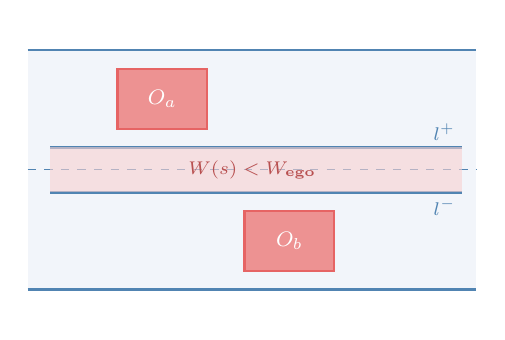
\begin{tikzpicture}[scale=0.95, transform shape]
  % 统一边界框：与子图 a/c 对齐
  \useasboundingbox (0,-1.9) rectangle (6.0,1.9);

  \fill[bglight] (0,-1.6) rectangle (6.0,1.6);
  \draw[deepblue, thick] (0,-1.6) -- (6.0,-1.6);
  \draw[deepblue, thick] (0, 1.6) -- (6.0, 1.6);
  \draw[deepblue, dashed, thin] (0,0) -- (6.0,0);

  \fill[obsstatic] (1.2,0.55) rectangle (2.4,1.35);
  \node[white, font=\footnotesize\bfseries] at (1.8,0.95) {$O_a$};

  \fill[obsstatic] (2.9,-1.35) rectangle (4.1,-0.55);
  \node[white, font=\footnotesize\bfseries] at (3.5,-0.95) {$O_b$};

  \draw[deepblue, very thick] (0.3,0.3) -- (5.8,0.3);
  \node[deepblue, font=\scriptsize, right] at (5.3,0.5) {$l^+$};

  \draw[deepblue, very thick] (0.3,-0.3) -- (5.8,-0.3);
  \node[deepblue, font=\scriptsize, right] at (5.3,-0.5) {$l^-$};

  \fill[dangerred!30, opacity=0.6] (0.3,-0.3) rectangle (5.8,0.3);
  \node[dangerred!80!black, font=\scriptsize\bfseries] at (3.0,0) {$W(s)<W_{\text{ego}}$};
\end{tikzpicture}
}
  \caption{独立决策矛盾}
  \label{fig:problem_overview:b}
\end{subfigure}

\vspace{0.6em}
\begin{subfigure}[b]{0.48\textwidth}
  \centering
  \resizebox{\linewidth}{!}{% 问题三 动态障碍物排除（子图 c）
\begin{tikzpicture}[scale=0.95, transform shape]
  % 统一边界框：与子图 a/b 对齐
  \useasboundingbox (0,-1.9) rectangle (6.0,1.9);

  % 道路
  \fill[bglight] (0,-1.8) rectangle (6.0,1.8);
  \draw[deepblue, thick] (0,-1.8) -- (6.0,-1.8);
  \draw[deepblue, thick] (0, 1.8) -- (6.0, 1.8);
  \draw[deepblue, dashed, thin] (0,0) -- (6.0,0);

  % 行人（动态障碍物）
  \fill[obsdyn] (3.5,0.1) rectangle (4.0,0.7);
  \draw[-Stealth, thick, dangerred] (3.75,0.7) -- (3.75,1.4);
  \node[font=\scriptsize, dangerred!70!black, right] at (4.1,1.15) {行人 1.2m/s};

  % Path阶段排除标记：× 叠在行人上，文字移到道路内右上方
  \node[dangerred, font=\Large, opacity=0.85] at (3.75,0.4) {\textbf{$\times$}};
  \node[font=\scriptsize, dangerred!80!black, right] at (4.1,0.4) {Path阶段排除};

  % 自车
  \fill[deepblue] (0.6,-0.35) rectangle (1.2,0.35);
  \node[deepblue, font=\tiny, below] at (0.9,-0.4) {自车};
  \draw[-Stealth, thick, deepblue] (1.3,0) -- (3.2,0);
  \node[font=\scriptsize, deepblue, above] at (2.25,0.05) {8 m/s};

  % Speed阶段才发现标注
  \draw[dangerred, very thick, dashed] (3.2,-0.6) rectangle (4.3,0.9);
  \node[dangerred, font=\scriptsize\bfseries] at (2.2,-1.25) {Speed阶段才发现};
  \draw[dangerred, thin] (3.0,-1.15) -- (3.2,-0.7);

\end{tikzpicture}
}
  \caption{动态障碍物排除}
  \label{fig:problem_overview:c}
\end{subfigure}
\caption{多障碍物场景三个核心问题的几何示意}
\label{fig:problem_overview}
\end{figure}

\section{安全裕度一刀切压缩通行空间}
\label{sec:problem_margin}

\subsection{问题描述}

PathBoundsDecider在构建路径边界时，需要在障碍物边缘外预留安全距离，以确保自车与障碍物之间保持足够的横向间距。该安全距离由\texttt{GetBuffer\-Between\-ADCCenter\-AndEdge}函数统一计算

\begin{lstlisting}[language=C++,caption={安全距离统一计算与nudge缓冲的静态/非静态分支},label={lst:buffer_calc}]
// path_bounds_decider_util.cc
// 相关 gflags 默认值（planning_gflags.cc）
//   obstacle_lat_buffer              = 0.4 m
//   static_obstacle_nudge_l_buffer   = 0.3 m
//   nonstatic_obstacle_nudge_l_buffer = 0.4 m
//   static_obstacle_speed_threshold  = 0.5 m/s

// 所有障碍物统一调用此函数计算安全距离
double PathBoundsDeciderUtil::
    GetBufferBetweenADCCenterAndEdge() {
  double adc_half_width =
      VehicleConfigHelper::GetConfig()
          .vehicle_param().width() / 2.0;
  return (adc_half_width + FLAGS_obstacle_lat_buffer);
}

// --- 静态/非静态的判定条件 ---
if (!obstacle.IsStatic() ||
    obstacle.speed() > FLAGS_static_obstacle_speed_threshold) {
  return false;  // 非静态障碍物不参与路径决策
}

// --- 边界松弛中的静态/非静态缓冲分支 ---
// 非静态障碍物使用 nonstatic buffer
double new_buffer = std::max(FLAGS_ego_front_slack_buffer,
                             FLAGS_nonstatic_obstacle_nudge_l_buffer);
// ...
// 静态障碍物使用 static buffer
if (path_bound_point->is_nudge_bound[LEFT_INDEX]) {
  old_buffer = std::max(FLAGS_obstacle_lat_buffer,
                        FLAGS_static_obstacle_nudge_l_buffer);
}
\end{lstlisting}

从代码可以看出，Apollo对安全距离的处理存在两个层面的粗粒度问题
\begin{enumerate}
\item \texttt{GetBufferBetweenADCCenterAndEdge}函数对所有障碍物返回相同的值，即半车宽加0.4\,m，完全不区分障碍物的类型、速度、横向偏移等特征。无论是远离车道的路锥、车道边缘的花坛，还是正对车道的违停车，均使用相同的安全距离。

\item Apollo虽然在\texttt{nudge\_l\_buffer}参数中区分了静态0.3\,m和非静态0.4\,m两个等级，但仅以0.5\,m/s的速度阈值做二分，低于该阈值视为静态，高于则视为非静态。该二分判定在 PathBoundsDecider 与 ObstacleNudgeDecider 的缓冲计算中通过 \texttt{!IsStatic() || speed() > FLAGS\_static\_obstacle\_speed\_threshold} 条件式生效。这种二分法无法区分运动方向随时突变的行人与轨迹可预测的同向行驶车辆，也无法区分碰撞时间短的正面接近障碍物与碰撞风险低的横向远离障碍物。
\end{enumerate}

\subsection{影响分析}

以下通过一个具体场景说明统一安全距离如何导致不必要的通行失败。定义净间距为道路边界到障碍物边缘之间扣除缓冲距离后的剩余宽度，自车可从某一侧通过当且仅当该侧净间距不小于自车宽度。

\textbf{场景设定}\quad 标准车道宽3.75\,m，$l_{road}^- = -1.875$\,m，$l_{road}^+ = 1.875$\,m。车道中偏右位置有一个路锥，横向占据$[-0.375,\; -0.075]$\,m，宽度0.3\,m。自车宽度$W_{ego} = 1.8$\,m。

\textbf{Apollo统一缓冲}\quad 取$d_{buf} = 0.3$\,m。从左侧通过时，净间距为
\[
1.875 - (-0.075) - 0.3 = 1.65\,\text{m} < W_{ego} = 1.8\,\text{m}
\]
从右侧通过时，净间距为
\[
(-0.375) - (-1.875) - 0.3 = 1.20\,\text{m} < 1.8\,\text{m}
\]
两侧均不足以容纳自车，路径被判定为BLOCKED，自车停车等待。

\textbf{差异化缓冲}\quad 该路锥处于静止状态且远离车道中心，威胁较低，取$d_{buf} = 0.15$\,m。从左侧通过时，净间距为
\[
1.875 - (-0.075) - 0.15 = 1.80\,\text{m} = W_{ego}
\]
恰好等于自车宽度，自车可从左侧安全通过。仅因缓冲参数从0.3\,m降至0.15\,m，净间距就从1.65\,m提升至1.80\,m，通行结果从BLOCKED翻转为可行。图\ref{fig:safety_margin_compression}直观对比了两种缓冲参数下的通行带差异。按障碍物威胁程度差异化分配安全距离的具体方法将在第五章展开。

\begin{figure}[H]
\centering
\resizebox{\textwidth}{!}{% 路锥场景：差异化 d_buf vs 统一 d_buf 对比
\begin{tikzpicture}[scale=1.0, transform shape]

% ============================================================
% 子图 (a)：差异化 d_buf=0.15m，恰好可通行
% ============================================================
\begin{scope}[shift={(0,0)}]
  % 背景
  \fill[bglight] (0,-2.3) rectangle (7.0,2.3);

  % 道路边界 ±1.875m
  \draw[deepblue, very thick] (0,-1.875) -- (7.0,-1.875);
  \draw[deepblue, very thick] (0, 1.875) -- (7.0, 1.875);
  \draw[deepblue, dashed, thin] (0,0) -- (7.0,0);

  % 车道宽度标注
  \draw[{Stealth}-{Stealth}, thin, deepblue] (0.3,-1.875) -- (0.3,1.875);
  \node[font=\scriptsize, deepblue, rotate=90] at (0.6,0) {车道 3.75m};

  % 路锥（宽0.3m，高0.3m，中心在 (3.25, -0.225)）
  % 横向 l: [-0.375, -0.075]，纵向 s: [3.1, 3.4]
  \fill[dangerred!70, draw=dangerred, thick] (3.1,-0.375) rectangle (3.4,-0.075);
  \node[white, font=\tiny\bfseries] at (3.25,-0.225) {锥};

  % 缓冲区 d_buf=0.15m（四周等距膨胀 0.15m）
  % l: [-0.375-0.15, -0.075+0.15] = [-0.525, 0.075]
  % s: [3.1-0.15, 3.4+0.15] = [2.95, 3.55]
  \draw[dangerred!70, dashed, thick] (2.95,-0.525) rectangle (3.55,0.075);
  \node[dangerred!70!black, font=\scriptsize, anchor=west] at (3.7,-0.225)
    {$\delta{=}0.15$m};

  % 膨胀距离标注（垂直）
  \draw[{Stealth}-{Stealth}, dangerred!60, thin] (2.8,-0.375) -- (2.8,-0.525);
  \node[dangerred!60, font=\tiny, left] at (2.75,-0.45) {0.15};
  \draw[{Stealth}-{Stealth}, dangerred!60, thin] (2.8,-0.075) -- (2.8,0.075);
  \node[dangerred!60, font=\tiny, left] at (2.75,0.0) {0.15};

  % 通行区域 [0.075, 1.875]（绿色填充）
  \fill[lightgreen, opacity=0.25] (1.0,0.075) rectangle (5.5,1.875);

  % 自车（宽1.8m = y方向，长4.5m = x方向，1:1比例）
  \fill[deepblue, opacity=0.3] (1.0,0.075) rectangle (5.5,1.875);
  \draw[deepblue, thick, rounded corners=2pt] (1.0,0.075) rectangle (5.5,1.875);
  \node[deepblue, font=\scriptsize\bfseries] at (3.25,0.975) {自车};

  % 净间距标注
  \draw[{Stealth}-{Stealth}, thick, lightgreen!60!black] (6.2,0.075) -- (6.2,1.875);
  \node[font=\scriptsize, lightgreen!60!black, anchor=west] at (6.3,0.975) {1.80m};
  \node[font=\scriptsize, lightgreen!60!black, anchor=west] at (6.3,0.55) {$= W_{\mathrm{ego}}$};

  \node[lightgreen!60!black, font=\normalsize\bfseries] at (1.5,-2.1) {\checkmark};

  % 子图标题
  \node[font=\small\bfseries, align=center] at (3.5,-2.7)
    {(a) $\delta{=}0.15$m（差异化），恰好可通行};
\end{scope}

% ============================================================
% 子图 (b)：Apollo d_buf=0.3m，BLOCKED
% ============================================================
\begin{scope}[shift={(8.5,0)}]
  % 背景
  \fill[bglight] (0,-2.3) rectangle (7.0,2.3);

  % 道路边界 ±1.875m
  \draw[deepblue, very thick] (0,-1.875) -- (7.0,-1.875);
  \draw[deepblue, very thick] (0, 1.875) -- (7.0, 1.875);
  \draw[deepblue, dashed, thin] (0,0) -- (7.0,0);

  % 车道宽度标注
  \draw[{Stealth}-{Stealth}, thin, deepblue] (0.3,-1.875) -- (0.3,1.875);
  \node[font=\scriptsize, deepblue, rotate=90] at (0.6,0) {车道 3.75m};

  % 路锥（同样大小）
  \fill[dangerred!70, draw=dangerred, thick] (3.1,-0.375) rectangle (3.4,-0.075);
  \node[white, font=\tiny\bfseries] at (3.25,-0.225) {锥};

  % 缓冲区 d_buf=0.3m（四周等距膨胀 0.3m）
  % l: [-0.375-0.3, -0.075+0.3] = [-0.675, 0.225]
  % s: [3.1-0.3, 3.4+0.3] = [2.8, 3.7]
  \draw[dangerred!70, dashed, thick] (2.8,-0.675) rectangle (3.7,0.225);
  \node[dangerred!70!black, font=\scriptsize, anchor=west] at (3.85,-0.225)
    {$\delta{=}0.3$m};

  % 膨胀距离标注
  \draw[{Stealth}-{Stealth}, dangerred!60, thin] (2.6,-0.375) -- (2.6,-0.675);
  \node[dangerred!60, font=\tiny, left] at (2.55,-0.525) {0.3};
  \draw[{Stealth}-{Stealth}, dangerred!60, thin] (2.6,-0.075) -- (2.6,0.225);
  \node[dangerred!60, font=\tiny, left] at (2.55,0.075) {0.3};

  % 上方不足区域 [0.225, 1.875] = 1.65m
  \fill[dangerred, opacity=0.12] (1.0,0.225) rectangle (5.5,1.875);
  % 下方不足区域 [-1.875, -0.675] = 1.2m
  \fill[dangerred, opacity=0.12] (1.0,-1.875) rectangle (5.5,-0.675);

  % 上方净间距
  \draw[{Stealth}-{Stealth}, thick, dangerred] (5.7,0.225) -- (5.7,1.875);
  \node[font=\scriptsize, dangerred, anchor=west] at (5.8,1.05) {1.65m};
  \node[font=\scriptsize, dangerred, anchor=west] at (5.8,0.65) {$< W_{\mathrm{ego}}$};

  % 下方净间距
  \draw[{Stealth}-{Stealth}, thick, dangerred] (5.7,-1.875) -- (5.7,-0.675);
  \node[font=\scriptsize, dangerred, anchor=west] at (5.8,-1.275) {1.20m};
  \node[font=\scriptsize, dangerred, anchor=west] at (5.8,-1.6) {$< W_{\mathrm{ego}}$};

  % BLOCKED
  \draw[dangerred, ultra thick] (2.5,1.0) -- (4.0,-1.0);
  \draw[dangerred, ultra thick] (2.5,-1.0) -- (4.0,1.0);
  \node[dangerred, font=\small\bfseries] at (3.25,-2.1) {BLOCKED};

  % 子图标题
  \node[font=\small\bfseries, align=center] at (3.5,-2.7)
    {(b) $\delta{=}0.3$m（统一），BLOCKED};
\end{scope}

\end{tikzpicture}
}
\caption{统一缓冲与差异化缓冲下的通行带对比}
\label{fig:safety_margin_compression}
\end{figure}

\section{SL层路径边界独立决策缺陷}
\label{sec:problem_sl}

\subsection{问题描述}

PathBoundsDecider是Apollo路径规划阶段的关键模块，负责在每个离散纵向位置$s$处构建横向路径边界$[l^-(s),\; l^+(s)]$。其核心缺陷在于对每个障碍物独立地决定避让方向（LEFT\_NUDGE或RIGHT\_NUDGE），而不考虑同一$s$截面上其他活跃障碍物的存在。当道路两侧同时存在障碍物时，这种逐障碍物的贪心决策可能产生相互矛盾的避让方向，即左侧障碍物使上边界下压、右侧障碍物使下边界上抬，导致$l^+(s) < l^-(s)$，路径边界被判定为BLOCKED，最终触发FallbackPath停车。

\subsection{源码定位与决策逻辑}

该问题的根源在于\texttt{UpdatePathBoundary\-BySLPolygon}函数。其核心逻辑包括三个环节，即逐障碍物独立决定避让方向、根据避让方向收缩路径边界、检测边界交叉并截断路径。代码\ref{lst:update_path_boundary}展示了该函数的关键流程。

\begin{lstlisting}[language=C++,caption={UpdatePathBoundaryBySLPolygon核心逻辑},label={lst:update_path_boundary}]
// path_bounds_decider_util.cc: UpdatePathBoundaryBySLPolygon
for (size_t i = 1; i < path_boundary->size(); ++i) {
  auto& left_bound = path_boundary->at(i).l_upper;   // 上边界
  auto& right_bound = path_boundary->at(i).l_lower;  // 下边界
  for (size_t j = 0; j < sl_polygon->size(); j++) {
    // --- 步骤1: 逐障碍物独立决定避让方向 ---
    if (sl_polygon->at(j).NudgeInfo() == SLPolygon::UNDEFINED) {
      double obs_l = (l_lower + l_upper) / 2;  // 障碍物中心横向位置
      if (is_passable_right && is_passable_left) {
        // 两侧均可通行时，根据障碍物中心与参考线的相对位置决定
        if (last_max_nudge_l < obs_l) {
          sl_polygon->at(j).SetNudgeInfo(SLPolygon::RIGHT_NUDGE);
        } else {
          sl_polygon->at(j).SetNudgeInfo(SLPolygon::LEFT_NUDGE);
        }
      } else if (is_passable_right) {
        sl_polygon->at(j).SetNudgeInfo(SLPolygon::RIGHT_NUDGE);
      } else {
        sl_polygon->at(j).SetNudgeInfo(SLPolygon::LEFT_NUDGE);
      }
    }
    // --- 步骤2: 根据避让方向更新边界 ---
    if (sl_polygon->at(j).NudgeInfo() == SLPolygon::RIGHT_NUDGE) {
      if (!sl_polygon->at(j).is_passable()[RIGHT_INDEX]) {
        sl_polygon->at(j).SetNudgeInfo(SLPolygon::BLOCKED);
        break;  // 右侧不可通行，标记BLOCKED
      }
      // 上边界收缩至障碍物左边缘减安全距离
      if (obs_right_nudge_bound.l_upper.l < left_bound.l) {
        left_bound.l = obs_right_nudge_bound.l_upper.l;
        left_bound.type = BoundType::OBSTACLE;
      }
    } else if (sl_polygon->at(j).NudgeInfo() == SLPolygon::LEFT_NUDGE) {
      if (!sl_polygon->at(j).is_passable()[LEFT_INDEX]) {
        sl_polygon->at(j).SetNudgeInfo(SLPolygon::BLOCKED);
        break;  // 左侧不可通行，标记BLOCKED
      }
      // 下边界上抬至障碍物右边缘加安全距离
      if (obs_left_nudge_bound.l_lower.l > right_bound.l) {
        right_bound.l = obs_left_nudge_bound.l_lower.l;
        right_bound.type = BoundType::OBSTACLE;
      }
    }
  }
  // --- 步骤3: BLOCKED判定与路径截断 ---
  if (!blocked_id->empty()) {
    TrimPathBounds(i, path_boundary);  // 截断后续路径边界
    return false;                      // 触发FallbackPath停车
  }
}
\end{lstlisting}

代码中步骤1，即第7至22行，展示了避让方向的独立决策，对每个在位置$s$处活跃的障碍物，通过\texttt{SetNudgeInfo}函数根据障碍物中心相对于参考线的横向位置独立决定\texttt{RIGHT\_NUDGE}，即从右侧绕行使上边界下压，或\texttt{LEFT\_NUDGE}，即从左侧绕行使下边界上抬。步骤2，即第23至44行，根据避让方向对路径边界进行收缩，其中安全距离\texttt{delta}由自车半宽，即\texttt{GetBufferBetweenADCCenterAndEdge}的返回值，与额外缓冲参数\texttt{obstacle\_lat\_buffer}相加得到。步骤3，即第46至49行，在上下边界交叉，即存在BLOCKED标记的障碍物时，调用\texttt{TrimPathBounds}清除后续路径边界并返回\texttt{false}，最终触发\texttt{FallbackPath}生成减速停车轨迹。

\subsection{失败模式分析}

以下通过一个对称场景说明独立决策如何导致不必要的停车。

\textbf{场景设定}\quad 双车道道路总宽7.5\,m，$l_{road}^- = -3.75$\,m，$l_{road}^+ = 3.75$\,m。在某纵向位置$s^*$处同时存在两个路锥，关于参考线近似对称

\begin{itemize}[noitemsep]
\item $O_a$偏右，横向占据$[0.1,\; 0.4]$\,m，中心$0.25$\,m
\item $O_b$偏左，横向占据$[-0.4,\; -0.1]$\,m，中心$-0.25$\,m
\end{itemize}

两个路锥均未越过车道中线，安全距离$\delta = 1.2$\,m。

\textbf{Apollo独立决策}\quad $O_a$中心$0.25 > 0$，分配RIGHT\_NUDGE，上边界收缩至
\[
l^+(s^*) = 0.1 - 1.2 = -1.1\,\text{m}
\]
$O_b$中心$-0.25 < 0$，分配LEFT\_NUDGE，下边界抬升至
\[
l^-(s^*) = -0.1 + 1.2 = 1.1\,\text{m}
\]
$l^+ = -1.1 < l^- = 1.1$，判定BLOCKED。贪心策略将自车挤入两个路锥之间仅0.2\,m的间隙，路径不可行，触发停车。

\textbf{全局统一决策}\quad 将两个路锥作为一组，统一分配RIGHT\_NUDGE，自车从两者右侧绕行
\[
l^+(s^*) = \min(0.1 - 1.2,\; -0.4 - 1.2) = -1.6\,\text{m}, \quad l^-(s^*) = -3.75\,\text{m}
\]
通行带宽度$W = -1.6 - (-3.75) = 2.15$\,m，自车可借用相邻车道从右侧安全通过。由对称性，统一LEFT\_NUDGE同样可行，$W = 3.75 - 1.6 = 2.15$\,m。

贪心策略将两个偏向不同侧的障碍物分别向内挤压，全局协调只需统一绕行方向，即可利用道路另一侧的充裕空间。当$k$个障碍物在同一纵向位置活跃时，避让方向共有$2^k$种组合，贪心策略只检查了其中一种，可能恰好选中不可行的组合而遗漏可行解。该问题的形式化建模与高效求解方法将在第五章详细展开。

图\ref{fig:path_conservative}直观展示了该场景中独立决策与全局协调的对比。

\begin{figure}[H]
\centering
\begin{subfigure}[b]{0.48\textwidth}
  \centering
  \resizebox{\linewidth}{!}{% 子图(a)：独立决策，矛盾避让 → BLOCKED
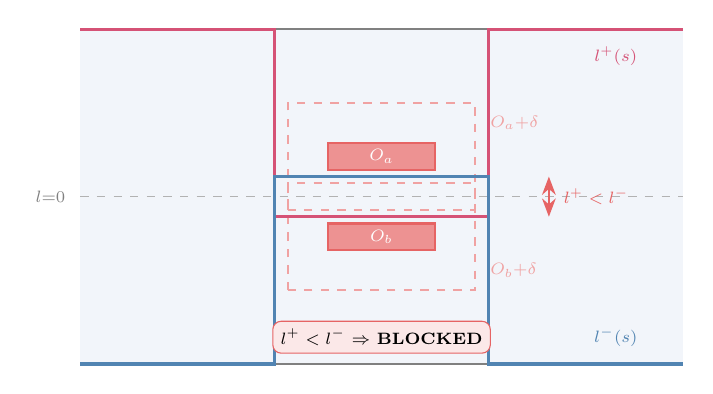
\begin{tikzpicture}[scale=0.85, transform shape]
  % 道路背景
  \fill[bglight] (-0.5,-2.5) rectangle (8.5,2.5);
  \draw[gray, thick] (-0.5, 2.5) -- (8.5, 2.5);
  \draw[gray, thick] (-0.5,-2.5) -- (8.5,-2.5);
  \draw[dashed, gray!60] (-0.5, 0) -- (8.5, 0);
  \node[gray, font=\scriptsize, anchor=east] at (-0.6, 0) {$l{=}0$};

  % O_a（上方）
  \fill[dangerred!70, draw=dangerred, thick] (3.2, 0.4) rectangle (4.8, 0.8);
  \node[font=\scriptsize, white] at (4.0, 0.6) {$O_a$};

  % O_b（下方）
  \fill[dangerred!70, draw=dangerred, thick] (3.2,-0.8) rectangle (4.8,-0.4);
  \node[font=\scriptsize, white] at (4.0,-0.6) {$O_b$};

  % 膨胀虚线 δ=0.6
  \draw[dangerred!60, dashed, thick] (2.6,-0.2) rectangle (5.4, 1.4);
  \node[dangerred!60, font=\scriptsize, anchor=west] at (5.5, 1.1) {$O_a{+}\delta$};
  \draw[dangerred!60, dashed, thick] (2.6,-1.4) rectangle (5.4, 0.2);
  \node[dangerred!60, font=\scriptsize, anchor=west] at (5.5,-1.1) {$O_b{+}\delta$};

  % 上界 l+(s)：右绕 O_a
  \draw[deeppink, very thick]
    (-0.5, 2.5) -- (2.4, 2.5) -- (2.4, -0.3) -- (5.6, -0.3) -- (5.6, 2.5) -- (8.5, 2.5);
  \node[deeppink, font=\scriptsize] at (7.5, 2.1) {$l^+(s)$};

  % 下界 l-(s)：左绕 O_b
  \draw[deepblue, very thick]
    (-0.5,-2.5) -- (2.4,-2.5) -- (2.4, 0.3) -- (5.6, 0.3) -- (5.6,-2.5) -- (8.5,-2.5);
  \node[deepblue, font=\scriptsize] at (7.5,-2.1) {$l^-(s)$};

  % 矛盾标注
  \draw[dangerred, thick, {Stealth}-{Stealth}] (6.5,-0.3) -- (6.5, 0.3);
  \node[dangerred, font=\scriptsize, anchor=west] at (6.6, 0) {$l^+ < l^-$};

  % BLOCKED 判定
  \node[draw=dangerred, fill=dangerred!15, font=\scriptsize,
        rounded corners=3pt, align=center] at (4.0,-2.1)
    {$l^+ < l^-$ $\Rightarrow$ \textbf{BLOCKED}};
\end{tikzpicture}
}
  \caption{独立决策，矛盾避让 $\to$ BLOCKED}
  \label{fig:path_conservative:a}
\end{subfigure}\hfill
\begin{subfigure}[b]{0.48\textwidth}
  \centering
  \resizebox{\linewidth}{!}{% 子图(b)：全局协调，统一右绕 → 通行
\begin{tikzpicture}[scale=0.85, transform shape]
  % 道路背景
  \fill[bglight] (-0.5,-2.5) rectangle (8.5,2.5);
  \draw[gray, thick] (-0.5, 2.5) -- (8.5, 2.5);
  \draw[gray, thick] (-0.5,-2.5) -- (8.5,-2.5);
  \draw[dashed, gray!60] (-0.5, 0) -- (8.5, 0);
  \node[gray, font=\scriptsize, anchor=east] at (-0.6, 0) {$l{=}0$};

  % O_a（上方）
  \fill[dangerred!70, draw=dangerred, thick] (3.2, 0.4) rectangle (4.8, 0.8);
  \node[font=\scriptsize, white] at (4.0, 0.6) {$O_a$};

  % O_b（下方）
  \fill[dangerred!70, draw=dangerred, thick] (3.2,-0.8) rectangle (4.8,-0.4);
  \node[font=\scriptsize, white] at (4.0,-0.6) {$O_b$};

  % 膨胀虚线 δ=0.6
  \draw[dangerred!60, dashed, thick] (2.6,-0.2) rectangle (5.4, 1.4);
  \node[dangerred!60, font=\scriptsize, anchor=west] at (5.5, 0.6) {$O_a{+}\delta$};
  \draw[dangerred!60, dashed, thick] (2.6,-1.4) rectangle (5.4, 0.2);
  \node[dangerred!60, font=\scriptsize, anchor=west] at (5.5,-0.6) {$O_b{+}\delta$};

  % 上界 l+(s)：统一右绕，压到 O_b 膨胀下缘
  \draw[deeppink, very thick]
    (-0.5, 2.5) -- (2.4, 2.5) -- (2.4, -1.5) -- (5.6, -1.5) -- (5.6, 2.5) -- (8.5, 2.5);
  \node[deeppink, font=\scriptsize] at (7.5, 2.1) {$l^+(s)$};

  % 下界 l-(s)：道路下界
  \draw[deepblue, very thick, dashed]
    (-0.5,-2.5) -- (8.5,-2.5);
  \node[deepblue, font=\scriptsize, left] at (-0.6,-2.5) {$l^-(s)$};

  % 通行带
  \fill[lightgreen, opacity=0.25] (-0.5,-2.5) rectangle (8.5,-1.5);

  % 通行带宽度标注
  \draw[deeppink, thick, {Stealth}-{Stealth}] (0.5,-2.5) -- (0.5,-1.5);
  \node[deeppink, font=\scriptsize, anchor=east] at (0.4,-2.0) {$W{=}1.0$m};

  % 自车轨迹
  \draw[deepblue, very thick, -{Stealth}]
    plot[smooth, tension=0.55] coordinates
      {(0.5, 0) (1.5,-0.5) (2.5,-1.8) (4.0,-2.0) (5.5,-1.8) (6.5,-0.5) (7.5, 0)};
  \node[deepblue, font=\scriptsize] at (4.0,-2.45) {规划轨迹};

  % PASS 判定
  \node[draw=lightgreen!80!black, fill=lightgreen!20, font=\scriptsize,
        rounded corners=3pt, align=center] at (4.0, 2.0)
    {统一右绕 $\Rightarrow$ \textbf{PASS}};
\end{tikzpicture}
}
  \caption{全局协调，统一右绕 $\to$ 通行}
  \label{fig:path_conservative:b}
\end{subfigure}
\caption{独立决策导致矛盾避让方向与全局协调的对比}
\label{fig:path_conservative}
\end{figure}

除了两个障碍物的极端情形外，随着障碍物数量增加，独立决策导致的可行域压缩会以近似指数方式恶化。图\ref{fig:feasible_compress}给出了同一车道内从2个、5个到极端密度障碍物场景下的可行域演化。在2个障碍物场景下，尚存较宽的可行通带可供自车选择，尽管贪心决策已开始压缩通带宽度；5个障碍物场景下，多次独立收缩使得可行域退化为断续的狭窄通带，任一处出现贪心矛盾即触发BLOCKED；极端密度场景下，可行域进一步碎片化，几乎任何贪心决策组合都会导致某处边界失效。这一演化揭示了问题二在高密度场景下的致命性，也量化说明了改进“决策粒度”对可行性恢复的杠杆效应远高于单纯调整安全裕度。

\begin{figure}[H]
\centering
\begin{subfigure}[b]{0.32\textwidth}
  \centering
  \resizebox{\linewidth}{!}{% 2 个障碍物 通行带可行（子图 a）
\begin{tikzpicture}[scale=0.7, transform shape]
  \draw[-Stealth, thick] (0,-2.5) -- (8.5,-2.5) node[right, font=\footnotesize] {$s$};
  \draw[-Stealth, thick] (0,-2.5) -- (0,2.5) node[above, font=\footnotesize] {$l$};

  \draw[gray, thick] (0,1.875) -- (8,1.875);
  \draw[gray, thick] (0,-1.875) -- (8,-1.875);
  \draw[gray, dashed] (0,0) -- (8,0);

  \begin{scope}[on background layer]
    \fill[bglight] (0,-1.875) rectangle (8,1.875);
  \end{scope}

  % O1（上方靠边）y=[0.6, 1.3], s=[2, 4]
  \fill[dangerred!70, draw=dangerred, thick] (2,0.6) rectangle (4,1.3);
  \node[white, font=\footnotesize\bfseries] at (3,0.95) {$O_1$};

  % O2（下方靠边）y=[-1.2, -0.5], s=[5, 7]
  \fill[dangerred!70, draw=dangerred, thick] (5,-1.2) rectangle (7,-0.5);
  \node[white, font=\footnotesize\bfseries] at (6,-0.85) {$O_2$};

  % O1 右绕 → 上界压到 O1 膨胀下缘 (0.6-0.4=0.2)
  \draw[deeppink, very thick]
    (0,1.875) -- (1.8,1.875) -- (1.8,0.2) -- (4.2,0.2) -- (4.2,1.875) -- (8,1.875);
  \node[deeppink, font=\tiny] at (1, 2.1) {$l^+(s)$};

  % O2 左绕 → 下界抬到 O2 膨胀上缘 (-0.5+0.4=-0.1)
  \draw[deepblue, very thick]
    (0,-1.875) -- (4.8,-1.875) -- (4.8,-0.1) -- (7.2,-0.1) -- (7.2,-1.875) -- (8,-1.875);
  \node[deepblue, font=\tiny] at (7.5, -2.1) {$l^-(s)$};

  \node[lightgreen!60!black, font=\footnotesize\bfseries] at (4,-1.35) {通行带充足};
\end{tikzpicture}
}
  \caption{2 个障碍物}
  \label{fig:feasible_compress:a}
\end{subfigure}\hfill
\begin{subfigure}[b]{0.32\textwidth}
  \centering
  \resizebox{\linewidth}{!}{% 4 个障碍物 通行带狭窄（子图 b）
\begin{tikzpicture}[scale=0.7, transform shape]
  \draw[-Stealth, thick] (0,-2.5) -- (8.5,-2.5) node[right, font=\footnotesize] {$s$};
  \draw[-Stealth, thick] (0,-2.5) -- (0,2.5) node[above, font=\footnotesize] {$l$};

  \draw[gray, thick] (0,1.875) -- (8,1.875);
  \draw[gray, thick] (0,-1.875) -- (8,-1.875);
  \draw[gray, dashed] (0,0) -- (8,0);

  \begin{scope}[on background layer]
    \fill[bglight] (0,-1.875) rectangle (8,1.875);
  \end{scope}

  % O1（上方靠边）y=[0.5, 1.1], s=[1, 2.5]
  \fill[dangerred!70, draw=dangerred, thick] (1,0.5) rectangle (2.5,1.1);
  \node[white, font=\tiny\bfseries] at (1.75,0.8) {$O_1$};

  % O2（下方靠边）y=[-1.0, -0.4], s=[2.5, 4]
  \fill[dangerred!70, draw=dangerred, thick] (2.5,-1.0) rectangle (4,-0.4);
  \node[white, font=\tiny\bfseries] at (3.25,-0.7) {$O_2$};

  % O3（上方靠边）y=[0.4, 0.9], s=[4.5, 6]
  \fill[dangerred!70, draw=dangerred, thick] (4.5,0.4) rectangle (6,0.9);
  \node[white, font=\tiny\bfseries] at (5.25,0.65) {$O_3$};

  % O4（下方靠边）y=[-0.8, -0.2], s=[6, 7.5]
  \fill[dangerred!70, draw=dangerred, thick] (6,-0.8) rectangle (7.5,-0.2);
  \node[white, font=\tiny\bfseries] at (6.75,-0.5) {$O_4$};

  % 上界 l+(s)：O1右绕压到0.1, O3右绕压到0.0
  \draw[deeppink, very thick]
    (0,1.875) -- (0.8,1.875) -- (0.8,0.1) -- (2.7,0.1)
    -- (2.7,1.875) -- (4.3,1.875) -- (4.3,0.0) -- (6.2,0.0)
    -- (6.2,1.875) -- (8,1.875);

  % 下界 l-(s)：O2左绕抬到0.0, O4左绕抬到0.2
  \draw[deepblue, very thick]
    (0,-1.875) -- (2.3,-1.875) -- (2.3,0.0) -- (4.2,0.0)
    -- (4.2,-1.875) -- (5.8,-1.875) -- (5.8,0.2) -- (7.7,0.2)
    -- (7.7,-1.875) -- (8,-1.875);

  % 窄处标注
  \draw[lightorange, ultra thick] (2.5,0.0) -- (2.5,0.1);
  \node[lightorange!80!black, font=\tiny\bfseries, anchor=west] at (2.6,0.05) {窄};
  \draw[lightorange, ultra thick] (6,0.0) -- (6,0.2);
  \node[lightorange!80!black, font=\tiny\bfseries, anchor=west] at (6.1,0.1) {窄};

  \node[deeppink, font=\tiny] at (0.5, 2.1) {$l^+(s)$};
  \node[deepblue, font=\tiny] at (7.5, -2.1) {$l^-(s)$};
  \node[lightorange!80!black, font=\footnotesize\bfseries] at (4,-1.5) {多次收缩 通行带退化};
\end{tikzpicture}
}
  \caption{4 个障碍物}
  \label{fig:feasible_compress:b}
\end{subfigure}\hfill
\begin{subfigure}[b]{0.32\textwidth}
  \centering
  \resizebox{\linewidth}{!}{% 密集障碍物 BLOCKED（子图 c）
\begin{tikzpicture}[scale=0.7, transform shape]
  \draw[-Stealth, thick] (0,-2.5) -- (8.5,-2.5) node[right, font=\footnotesize] {$s$};
  \draw[-Stealth, thick] (0,-2.5) -- (0,2.5) node[above, font=\footnotesize] {$l$};

  \draw[gray, thick] (0,1.875) -- (8,1.875);
  \draw[gray, thick] (0,-1.875) -- (8,-1.875);
  \draw[gray, dashed] (0,0) -- (8,0);

  \begin{scope}[on background layer]
    \fill[bglight] (0,-1.875) rectangle (8,1.875);
  \end{scope}

  % 密集障碍物（交替上下，靠近道路边缘）
  \fill[dangerred!70, draw=dangerred, thick] (0.5,0.4) rectangle (1.5,1.2);
  \node[white, font=\tiny\bfseries] at (1,0.8) {$O_1$};

  \fill[dangerred!70, draw=dangerred, thick] (1.5,-1.1) rectangle (2.5,-0.3);
  \node[white, font=\tiny\bfseries] at (2,-0.7) {$O_2$};

  \fill[dangerred!70, draw=dangerred, thick] (2.5,0.3) rectangle (3.5,1.1);
  \node[white, font=\tiny\bfseries] at (3,0.7) {$O_3$};

  \fill[dangerred!70, draw=dangerred, thick] (3.5,-1.0) rectangle (4.5,-0.2);
  \node[white, font=\tiny\bfseries] at (4,-0.6) {$O_4$};

  \fill[dangerred!70, draw=dangerred, thick] (4.5,0.5) rectangle (5.5,1.3);
  \node[white, font=\tiny\bfseries] at (5,0.9) {$O_5$};

  \fill[dangerred!70, draw=dangerred, thick] (5.5,-1.2) rectangle (6.5,-0.3);
  \node[white, font=\tiny\bfseries] at (6,-0.75) {$O_6$};

  \fill[dangerred!70, draw=dangerred, thick] (6.5,0.3) rectangle (7.5,1.1);
  \node[white, font=\tiny\bfseries] at (7,0.7) {$O_7$};

  % 上界 l+(s)：逐步压低 (δ=0.4)
  \draw[deeppink, very thick]
    (0,1.875) -- (0.3,1.875) -- (0.3,0.0) -- (1.7,0.0)
    -- (1.7,1.875) -- (2.3,1.875) -- (2.3,-0.1) -- (3.7,-0.1)
    -- (3.7,1.875) -- (4.3,1.875) -- (4.3,0.1) -- (5.7,0.1);

  % 下界 l-(s)：逐步抬高
  \draw[deepblue, very thick]
    (0,-1.875) -- (1.3,-1.875) -- (1.3,0.1) -- (2.7,0.1)
    -- (2.7,-1.875) -- (3.3,-1.875) -- (3.3,0.2) -- (4.7,0.2);

  % BLOCKED 点
  \fill[dangerred] (4.5,0.15) circle (3pt);

  % 截断区域
  \fill[dangerred, opacity=0.1] (4.5,-1.875) rectangle (8,1.875);
  \node[dangerred, font=\footnotesize\bfseries] at (6.5,1.3) {$l^+ < l^- \rightarrow$ BLOCKED};
  \node[dangerred, font=\tiny] at (6.5,-1.5) {TrimPathBounds 截断};

  \node[deeppink, font=\tiny] at (0.5, 2.1) {$l^+(s)$};
  \node[deepblue, font=\tiny] at (0.5, -2.1) {$l^-(s)$};
\end{tikzpicture}
}
  \caption{密集障碍物}
  \label{fig:feasible_compress:c}
\end{subfigure}
\caption{多障碍物场景下可行域的退化演化}
\label{fig:feasible_compress}
\end{figure}

\subsection{BLOCKED后的截断与恢复机制局限}

当PathBoundsDecider判定BLOCKED后，调用\texttt{TrimPathBounds}截断路径

\begin{lstlisting}[language=C++,caption={TrimPathBounds路径截断},label={lst:trim_path}]
// path_bounds_decider_util.cc: TrimPathBounds
void PathBoundsDeciderUtil::TrimPathBounds(
    const int path_blocked_idx, PathBoundary* const path_boundaries) {
  if (path_blocked_idx != -1) {
    if (path_blocked_idx == 0) {
      AINFO << "Completely blocked. Cannot move at all.";
    }
    double front_edge_to_center =
        VehicleConfigHelper::GetConfig().vehicle_param().front_edge_to_center();
    double trimmed_s =
        path_boundaries->at(path_blocked_idx).s - front_edge_to_center;
    while (path_boundaries->size() > 1 &&
           path_boundaries->back().s > trimmed_s) {
      path_boundaries->pop_back();  // 逐个弹出BLOCKED位置之后的边界点
    }
  }
}
\end{lstlisting}

该函数将路径边界截断至BLOCKED位置的前方，即减去车头到中心的距离，后续的\texttt{FallbackPath}模块基于截断后的短路径生成减速停车轨迹。整个过程是不可逆的，一旦某个避让方向组合导致BLOCKED，系统不会回溯尝试其他方向组合，而是直接进入停车流程。

Apollo提供的\texttt{LaneBorrowPath}机制可以在一定条件下缓解BLOCKED问题，但该机制的触发条件非常严格。代码\ref{lst:lane_borrow_conditions}展示了借道决策需要通过的5个前置检查及条件4的具体实现

\begin{lstlisting}[language=C++,caption={LaneBorrowPath的前置条件与长期阻塞判定},label={lst:lane_borrow_conditions}]
// lane_borrow_path.cc: IsNecessaryToBorrowLane
// 条件1: 仅单参考线场景（路口等多参考线场景不借道）
if (!HasSingleReferenceLine(*frame_)) { return false; }
// 条件2: 自车速度低于阈值（默认5.0 m/s）
if (!IsWithinSidePassingSpeedADC(*frame_)) { return false; }
// 条件3: 阻塞障碍物远离路口
if (!IsBlockingObstacleFarFromIntersection(*ref_info)) { return false; }
// 条件4: 障碍物持续阻塞达到cycle阈值（默认3个周期）
if (!IsLongTermBlockingObstacle()) { return false; }
// 条件5: 阻塞障碍物在目的地范围内
if (!IsBlockingObstacleWithinDestination(*ref_info)) { return false; }

// 条件4的具体实现: IsLongTermBlockingObstacle
bool LaneBorrowPath::IsLongTermBlockingObstacle() {
  if (injector_->planning_context()->planning_status().path_decider()
          .front_static_obstacle_cycle_counter() >=
      config_.long_term_blocking_obstacle_cycle_threshold()) {  // 默认值: 3
    return true;
  }
  return false;
}
\end{lstlisting}

这意味着：即使存在可行的借道方案，系统也必须先经历至少3个规划周期，约300\,ms，的停车等待才会尝试借道；且借道仅在单参考线、低速、远离路口等条件同时满足时才被允许。在路口附近、高速行驶、或多参考线场景下，LaneBorrow机制不会触发，BLOCKED判定将直接导致停车。

\section{ST层路径-速度协调缺失}
\label{sec:problem_st}

\subsection{问题描述与源码定位}

\textbf{问题}\quad{}Apollo的路径决策模块在确定障碍物的避让方向时，完全排除了动态障碍物。所有非静态障碍物，包括行驶中的车辆、行走的行人、骑行的自行车等，不参与PathBoundsDecider的边界构建，而是被完全交给速度规划阶段的ST图处理。这意味着路径规划阶段看到的“世界”中只有静态障碍物，动态障碍物如同不存在。

\textbf{源码定位}\quad{}该问题的源码证据体现在\texttt{IsWithinPathDecider\-ScopeObstacle}函数中

\begin{lstlisting}[language=C++,caption={动态障碍物被路径决策排除},label={lst:scope_obstacle}]
// path_bounds_decider_util.cc: IsWithinPathDeciderScopeObstacle
bool PathBoundsDeciderUtil::IsWithinPathDeciderScopeObstacle(
    const Obstacle& obstacle) {
  // 虚拟障碍物不参与路径决策
  if (obstacle.IsVirtual()) {
    return false;
  }
  // 已有IGNORE决策的障碍物跳过
  if (obstacle.HasLongitudinalDecision() && obstacle.HasLateralDecision()
      && obstacle.IsIgnore()) {
    return false;
  }
  // 非静态障碍物或速度超过阈值的障碍物直接排除
  if (!obstacle.IsStatic() ||
      obstacle.speed() > FLAGS_static_obstacle_speed_threshold) {
    return false;  // 动态障碍物不参与路径决策
  }
  // TODO(jiacheng):
  // Some obstacles are not moving, but only because they are waiting
  // for red light (traffic rule) or because they are blocked by
  // others (social). These obstacles will almost certainly move in
  // the near future and we should not side-pass such obstacles.
  return true;
}
\end{lstlisting}

值得注意的是，Apollo开发团队在该函数中留下了\texttt{TODO}注释，表明他们意识到当前的处理方式存在不足，但尚未实施改进。这个\texttt{TODO}注释本身就是该问题存在的直接证据。

\subsection{影响分析}

动态障碍物被排除在路径决策之外，产生以下影响。

\textbf{影响一}，路径与速度规划之间缺乏协调

在Apollo的路径-速度解耦架构中，如第三章3.3节所述，路径规划先于速度规划执行，速度规划在路径规划的结果上构建ST图。当动态障碍物不参与路径决策时，路径阶段可能生成一条直行路径，而速度阶段在该路径上发现动态障碍物横穿，不得不急刹或停车等待。如果路径阶段考虑了动态障碍物的预测轨迹，完全可以提前规划一条避让路径，在保持速度的同时安全通过。

\textbf{影响二}，横穿行人在路径规划中完全不存在

考虑一个典型场景：一名行人正在从右向左横穿道路。在路径规划阶段，由于该行人是动态障碍物（\texttt{IsStatic() == false}），PathBoundsDecider完全忽略其存在，路径规划生成的是一条沿车道中心线的直行路径。随后速度规划在ST图中检测到该行人的ST边界，只能通过减速或停车来避让。

具体地，设自车以$v_{ego} = 8$\,m/s行驶，前方$s = 10$\,m处一名行人以$v_{lat} = 1.2$\,m/s从右向左横穿，当前位于车道中央$l = 0$处。自车到达该位置需$t = 10/8 = 1.25$\,s，届时行人已横移$1.2 \times 1.25 = 1.5$\,m，移至$l = 1.5$\,m处，接近车道左边缘。如果路径规划阶段纳入行人的预测轨迹，可以基于行人在$t = 1.25$\,s时的预测位置（$l = 1.5$\,m）计算路径边界，此时行人已不在车道中央，自车可从行人右侧安全通过，无需停车。但由于行人被\texttt{IsWithinPathDeciderScopeObstacle}过滤，路径阶段对此一无所知，速度阶段只能被迫停车等待。该场景的完整时变分析将在第五章中给出。

图\ref{fig:dynamic_exclusion}给出了该场景下行人时变位置与自车到达时刻的三帧对比。子图(a)为$t=0$时刻，自车刚开始规划，行人距自车10\,m，尚未进入车道，PathBoundsDecider看到的“世界”中该行人不存在。子图(b)为$t=0.625$\,s时刻，自车已行进5\,m，行人横移0.75\,m进入车道右半侧，恰好落在自车直行路径上形成碰撞窗口。子图(c)为$t=1.25$\,s时刻，行人已穿过车道抵达对侧，自车到达原障碍位置时路径已然通畅。若Path阶段能够利用行人的预测轨迹即“在自车到达该位置时行人已横移1.5\,m至车道边缘”这一事实，完全可以在规划初始即选择从行人右侧绕行或保持直行，无需进入Speed阶段的急刹降级。

\begin{figure}[H]
\centering
\begin{subfigure}[b]{0.32\textwidth}
  \centering
  \resizebox{\linewidth}{!}{% 动态障碍物排除 t=0 时刻（子图 a）
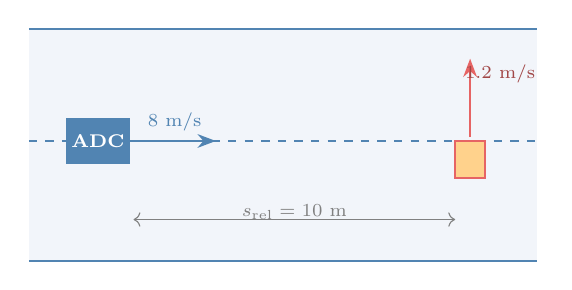
\begin{tikzpicture}[scale=0.95, transform shape]
  \fill[bglight] (0,-1.3) rectangle (6.8,1.8);
  \draw[deepblue, thick] (0,-1.3) -- (6.8,-1.3);
  \draw[deepblue, thick] (0, 1.8) -- (6.8, 1.8);
  \draw[deepblue, dashed, thin] (0,0.3) -- (6.8,0.3);

  \fill[egopt] (0.5,0) rectangle (1.35,0.6);
  \node[white, font=\scriptsize\bfseries] at (0.925,0.3) {ADC};
  \draw[-Stealth, thick, deepblue] (1.4,0.3) -- (2.5,0.3);
  \node[font=\scriptsize, deepblue] at (1.95,0.55) {8 m/s};

  \fill[obsdyn] (5.7,-0.2) rectangle (6.1,0.3);
  \draw[-Stealth, thick, dangerred] (5.9,0.35) -- (5.9,1.4);
  \node[font=\scriptsize, dangerred!70!black] at (6.3,1.2) {1.2 m/s};

  \draw[<->, thin, gray] (1.4,-0.75) -- (5.7,-0.75);
  \node[font=\scriptsize, gray] at (3.55,-0.65) {$s_{\text{rel}}=10$ m};
\end{tikzpicture}
}
  \caption{$t=0$ 行人未进入路径}
  \label{fig:dynamic_exclusion:a}
\end{subfigure}\hfill
\begin{subfigure}[b]{0.32\textwidth}
  \centering
  \resizebox{\linewidth}{!}{% 动态障碍物排除 t=0.625s（子图 b）
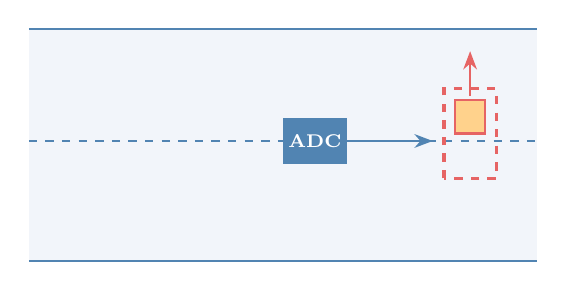
\begin{tikzpicture}[scale=0.95, transform shape]
  \fill[bglight] (0,-1.3) rectangle (6.8,1.8);
  \draw[deepblue, thick] (0,-1.3) -- (6.8,-1.3);
  \draw[deepblue, thick] (0, 1.8) -- (6.8, 1.8);
  \draw[deepblue, dashed, thin] (0,0.3) -- (6.8,0.3);

  \fill[egopt] (3.4,0) rectangle (4.25,0.6);
  \node[white, font=\scriptsize\bfseries] at (3.825,0.3) {ADC};
  \draw[-Stealth, thick, deepblue] (4.3,0.3) -- (5.4,0.3);

  \fill[obsdyn] (5.7,0.4) rectangle (6.1,0.85);
  \draw[-Stealth, thick, dangerred] (5.9,0.9) -- (5.9,1.5);

  \draw[dangerred, very thick, dashed] (5.55,-0.2) rectangle (6.25,1.0);
\end{tikzpicture}
}
  \caption{$t=0.625$ s 行人半入路径}
  \label{fig:dynamic_exclusion:b}
\end{subfigure}\hfill
\begin{subfigure}[b]{0.32\textwidth}
  \centering
  \resizebox{\linewidth}{!}{% 动态障碍物排除 t=1.25s（子图 c）
\begin{tikzpicture}[scale=0.95, transform shape]
  \fill[bglight] (0,-1.3) rectangle (6.8,1.8);
  \draw[deepblue, thick] (0,-1.3) -- (6.8,-1.3);
  \draw[deepblue, thick] (0, 1.8) -- (6.8, 1.8);
  \draw[deepblue, dashed, thin] (0,0.3) -- (6.8,0.3);

  \fill[egopt, opacity=0.3] (0.5,0) rectangle (1.35,0.6);
  \node[gray, font=\scriptsize] at (0.925,0.3) {$t=0$};

  \fill[egopt] (5.7,0) rectangle (6.55,0.6);
  \node[white, font=\scriptsize\bfseries] at (6.125,0.3) {ADC};

  \fill[obsdyn] (5.7,1.3) rectangle (6.1,1.75);
  \node[font=\scriptsize, dangerred!70!black, above] at (5.9,1.8) {已穿过};

  \fill[bandok] (1.5,0.05) rectangle (5.6,0.55);
  \node[font=\scriptsize, lightgreen!50!black] at (3.5,0.3) {路径已打开};
\end{tikzpicture}
}
  \caption{$t=1.25$ s 路径通畅}
  \label{fig:dynamic_exclusion:c}
\end{subfigure}
\caption{动态障碍物排除后的时变演化示意}
\label{fig:dynamic_exclusion}
\end{figure}

\textbf{影响三}，加剧问题一的影响

动态障碍物的排除使得PathBoundsDecider只能基于障碍物在$t = 0$时刻的静态快照做决策，无法利用时间维度的信息。例如，一辆缓慢移动的车辆在当前时刻$t = 0$占据车道中央，但$t = 2$s后将移至车道边缘甚至离开车道。如果纳入该动态障碍物的预测轨迹，PathBoundsDecider可以基于自车到达该$s$位置时障碍物的预测位置来决定避让方向，而非基于其当前位置。这种时间维度的利用可以显著减少问题一中BLOCKED判定的发生频率。

\subsection{PathDecider中的同一问题}

不仅PathBoundsDecider排除动态障碍物，路径决策器PathDecider同样如此。

\begin{lstlisting}[language=C++,caption={PathDecider同样排除动态障碍物},label={lst:path_decider_static}]
// path_decider.cc: MakeStaticObstacleDecision
for (const auto *obstacle : path_decision->obstacles().Items()) {
  // 跳过非静态障碍物和虚拟障碍物
  if (!obstacle->IsStatic() || obstacle->IsVirtual()) {
    continue;
  }
  // 已有IGNORE决策的障碍物跳过
  if (obstacle->HasLongitudinalDecision() &&
      obstacle->LongitudinalDecision().has_ignore() &&
      obstacle->HasLateralDecision() &&
      obstacle->LateralDecision().has_ignore()) {
    continue;
  }
  // ... 后续仅对静态障碍物执行STOP/NUDGE/IGNORE决策
}
\end{lstlisting}

可以看到，\texttt{MakeStaticObstacleDecision}在遍历障碍物列表的第一步即通过\texttt{IsStatic()}过滤掉所有动态障碍物。这意味着Apollo路径规划阶段的两个核心决策模块，即负责构建横向边界的PathBoundsDecider和负责做出STOP/NUDGE/IGNORE决策的PathDecider，都将动态障碍物完全排除在外，形成了系统性的路径-速度协调缺失。

\subsection{路径决策信息未传递至速度规划}

除了动态障碍物被排除外，ST层面还存在一个更深层的问题，路径决策阶段产生的时空信息没有传递给速度规划阶段。

在Apollo的路径-速度解耦架构中，PathBoundsDecider输出的是横向路径边界$[l^-(s), l^+(s)]$，SpeedBoundsDecider基于该路径独立构建ST边界。两个模块之间的信息传递是单向的、有限的，速度规划知道路径在哪里，但不知道路径为什么在那里。

这种信息断层的后果在动态障碍物场景中尤为明显。考虑改进后的路径规划，路径决策可能基于“行人将在$t = 1.25$\,s后移开”这一预判选择了一条通过方案，但SpeedBoundsDecider不知道这一时间约束的存在。如果速度规划恰好让自车在行人移开之前到达该位置，路径决策的前提条件就被违反了。

因此，ST层面的问题不仅是“排除了动态障碍物”，更本质的问题是路径规划和速度规划之间缺乏时空约束的传递通道。改进方案需要建立这样一个通道，路径层面的时变决策能够以约束的形式传递给速度层面，确保两者的一致性。图\ref{fig:path_speed_breakage}示意了现有架构中路径阶段到速度阶段的单向信息流以及缺失的时空一致性反向通道。

\begin{figure}[H]
\centering
\resizebox{0.8\textwidth}{!}{% 路径与速度规划之间的单向信息传递与时空约束缺口
\begin{tikzpicture}[scale=0.95, transform shape,
    infobox/.style={rectangle, rounded corners=4pt, draw=deepblue, fill=lightblue!30,
        minimum width=3.8cm, align=left, font=\small, inner sep=8pt},
    recvbox/.style={rectangle, rounded corners=4pt, draw=deepblue, fill=bglight,
        minimum width=3.8cm, align=left, font=\small, inner sep=8pt},
    lostitem/.style={rectangle, rounded corners=2pt, draw=dangerred!70, fill=dangerred!8,
        font=\small, inner sep=4pt},
]

% ===== Left: Path 阶段产生的决策信息 =====
\node[infobox, minimum height=3.8cm] (pathbox) at (0, 0) {%
    \textbf{Path 阶段产生的决策信息}\\[5pt]
    \textcolor{deepblue}{\textbullet}~避让方向 $d_i$\\[3pt]
    \textcolor{deepblue}{\textbullet}~横向边界 $[l^-(s),\,l^+(s)]$\\[3pt]
    \textcolor{deepblue}{\textbullet}~时间前提 $t_{\mathrm{clear}}$\\[3pt]
    \textcolor{deepblue}{\textbullet}~威胁度评估 $\theta_i$%
};

% ===== Right: Speed 阶段接收的信息 =====
\node[recvbox, minimum height=3.0cm] (speedbox) at (11.5, 0) {%
    \textbf{Speed 阶段接收的信息}\\[5pt]
    \textcolor{deepblue}{\textbullet}\;$[l^-(s),\,l^+(s)]$\\[1pt]
    {\footnotesize\textcolor{deepblue}{知道路径在哪里}}\\[6pt]
    \textcolor{dangerred}{\texttimes}\;$d_i,\;t_{\mathrm{clear}},\;\theta_i$\\[1pt]
    {\footnotesize\textcolor{dangerred}{不知道路径为什么在那里}}%
};

% ===== Middle: 传递瓶颈（漏斗形，内部干净） =====
\coordinate (fTL) at (4.6, 1.9);
\coordinate (fBL) at (4.6,-1.9);
\coordinate (fTR) at (7.8, 0.55);
\coordinate (fBR) at (7.8,-0.55);

\fill[bglight, draw=deepblue!60, thick]
    (fTL) -- (fTR) -- (fBR) -- (fBL) -- cycle;

\node[font=\small\bfseries, deepblue!80] at (6.1, 2.3) {传递瓶颈};

% 一根蓝色箭头从 pathbox 穿过漏斗到 speedbox
\draw[deepblue, very thick, -Stealth] (pathbox.east) -- (speedbox.west)
    node[midway, above, font=\small\bfseries, deepblue] {$[l^-(s),\,l^+(s)]$};

% ===== 丢失的信息：漏斗上下方标注，箭头撞向漏斗壁 =====
% 上方
\node[lostitem] (ld) at (5.0, 3.2) {$d_i$\;避让方向};
\node[lostitem] (lt) at (8.0, 3.2) {$t_{\mathrm{clear}}$\;时间前提};
\draw[dangerred, thick, -|] (ld.south) -- ($(fTL)!0.2!(fTR)$)
    node[pos=0.4, right, font=\small\bfseries, dangerred] {\texttimes};
\draw[dangerred, thick, -|] (lt.south) -- ($(fTL)!0.7!(fTR)$)
    node[pos=0.4, right, font=\small\bfseries, dangerred] {\texttimes};

% 下方
\node[lostitem] (lth) at (6.3, -3.2) {$\theta_i$\;威胁度评估};
\draw[dangerred, thick, -|] (lth.north) -- ($(fBL)!0.4!(fBR)$)
    node[pos=0.4, right, font=\small\bfseries, dangerred] {\texttimes};

\end{tikzpicture}
}
\caption{路径与速度规划之间的单向信息传递与时空约束缺口}
\caption*{\scriptsize 图中漏斗表示两阶段之间的信息瓶颈。Path阶段产生的避让方向$d_i$、时间前提$t_{\mathrm{clear}}$和威胁度$\theta_i$均未传递至Speed阶段，仅横向边界$[l^-(s),l^+(s)]$通过。}
\label{fig:path_speed_breakage}
\end{figure}

\section{问题总结与改进方向}
\label{sec:problem_relation}

表\ref{tab:problem_summary}对比了三个问题的特征及其对应的改进方向。

\begin{table}[htbp]
\centering
\caption{多障碍物场景三个核心问题与改进方向}
\label{tab:problem_summary}
\small
\begin{tabularx}{\textwidth}{lXXX}
\toprule
& \textbf{问题一\quad 安全裕度一刀切} & \textbf{问题二\quad 独立决策} & \textbf{问题三\quad 动态障碍物排除} \\
\midrule
\textbf{涉及模块} & PathBoundsDecider & PathBoundsDecider & PathBoundsDecider / PathDecider \\
\textbf{根源} & 统一安全距离不区分威胁 & 逐障碍物贪心决策 & 动态障碍物不参与路径决策 \\
\textbf{表现} & 通行带被不必要压缩 & 路径BLOCKED $\rightarrow$ 停车 & 错过时变可行方案 \\
\textbf{严重程度} & 严重，加剧问题二 & 致命 & 严重，加剧问题二 \\
\textbf{改进维度} & 差异化安全距离 & 全局协调决策 & 时空约束协调 \\
\bottomrule
\end{tabularx}
\end{table}

表中“严重程度”一列反映了三个问题的相对权重，问题二是导致路径BLOCKED的直接瓶颈，问题一和问题三则分别从安全距离维度和时间维度提高问题二的发生概率。三个改进维度在数学上可纳入一个统一的优化框架，具体的问题建模与算法设计见第五章。

\section{本章小结}

本章分析了Apollo在多障碍物场景下的三个核心规划缺陷。问题一，所有障碍物使用统一的安全距离，不区分威胁程度，不必要地压缩通行空间。问题二，PathBoundsDecider对每个障碍物独立决定避让方向，在道路两侧同时存在障碍物时产生矛盾决策，导致路径BLOCKED。问题三，动态障碍物被完全排除在路径决策之外，Apollo团队在源码中留下的\texttt{TODO}注释证实了这一缺陷，且路径-速度之间缺乏时空约束传递通道。三个问题分别从安全距离、决策粒度和时空协调三个维度指向相应的改进方向，具体的算法设计与实现见第五章。

\chapter{多因子威胁度与差异化安全距离}

本章对应GTOC的第一项改进，针对Apollo PathBoundsDecider对所有障碍物使用统一安全距离的设计缺陷，提出基于多因子威胁度评估的差异化安全裕度$\delta_i$分配机制。本章首先深入剖析Apollo一刀切缓冲在多障碍物场景下压缩通行空间的源码根源与几何后果，进而设计融合TTC、横向重叠率、相对速度、障碍物类型与交互密度五个因子的威胁度评估模型，并将其映射为差异化的安全裕度。差异化$\delta_i$将作为基础量被第六章的最大间隙公式与第七章的时空走廊边界共同采用。

\section{安全裕度一刀切压缩通行空间}
\label{sec:problem_margin}

\subsection{问题描述}

PathBoundsDecider在构建路径边界时，需要在障碍物边缘外预留安全距离，以确保自车与障碍物之间保持足够的横向间距。该安全距离由\texttt{GetBuffer\-Between\-ADCCenter\-AndEdge}函数统一计算

\begin{lstlisting}[language=C++,caption={安全距离统一计算与nudge缓冲的静态/非静态分支},label={lst:buffer_calc}]
// path_bounds_decider_util.cc
// 相关 gflags 默认值（planning_gflags.cc）
//   obstacle_lat_buffer              = 0.4 m
//   static_obstacle_nudge_l_buffer   = 0.3 m
//   nonstatic_obstacle_nudge_l_buffer = 0.4 m
//   static_obstacle_speed_threshold  = 0.5 m/s

// 所有障碍物统一调用此函数计算安全距离
double PathBoundsDeciderUtil::
    GetBufferBetweenADCCenterAndEdge() {
  double adc_half_width =
      VehicleConfigHelper::GetConfig()
          .vehicle_param().width() / 2.0;
  return (adc_half_width + FLAGS_obstacle_lat_buffer);
}

// --- 静态/非静态的判定条件 ---
if (!obstacle.IsStatic() ||
    obstacle.speed() > FLAGS_static_obstacle_speed_threshold) {
  return false;  // 非静态障碍物不参与路径决策
}

// --- 边界松弛中的静态/非静态缓冲分支 ---
// 非静态障碍物使用 nonstatic buffer
double new_buffer = std::max(FLAGS_ego_front_slack_buffer,
                             FLAGS_nonstatic_obstacle_nudge_l_buffer);
// ...
// 静态障碍物使用 static buffer
if (path_bound_point->is_nudge_bound[LEFT_INDEX]) {
  old_buffer = std::max(FLAGS_obstacle_lat_buffer,
                        FLAGS_static_obstacle_nudge_l_buffer);
}
\end{lstlisting}

从代码可以看出，Apollo对安全距离的处理存在两个层面的粗粒度问题
\begin{enumerate}
\item \texttt{GetBufferBetweenADCCenterAndEdge}函数对所有障碍物返回相同的值，即半车宽加0.4\,m，完全不区分障碍物的类型、速度、横向偏移等特征。无论是远离车道的路锥、车道边缘的花坛，还是正对车道的违停车，均使用相同的安全距离。

\item Apollo虽然在\texttt{nudge\_l\_buffer}参数中区分了静态0.3\,m和非静态0.4\,m两个等级，但仅以0.5\,m/s的速度阈值做二分，低于该阈值视为静态，高于则视为非静态。该二分判定在 PathBoundsDecider 与 ObstacleNudgeDecider 的缓冲计算中通过 \texttt{!IsStatic() || speed() > FLAGS\_static\_obstacle\_speed\_threshold} 条件式生效。这种二分法无法区分运动方向随时突变的行人与轨迹可预测的同向行驶车辆，也无法区分碰撞时间短的正面接近障碍物与碰撞风险低的横向远离障碍物。
\end{enumerate}

\subsection{影响分析}

以下通过一个具体场景说明统一安全距离如何导致不必要的通行失败。定义净间距为道路边界到障碍物边缘之间扣除缓冲距离后的剩余宽度，自车可从某一侧通过当且仅当该侧净间距不小于自车宽度。

\textbf{场景设定}\quad 标准车道宽3.75\,m，$l_{road}^- = -1.875$\,m，$l_{road}^+ = 1.875$\,m。车道中偏右位置有一个路锥，横向占据$[-0.375,\; -0.075]$\,m，宽度0.3\,m。自车宽度$W_{ego} = 1.8$\,m。

\textbf{Apollo统一缓冲}\quad 取$d_{buf} = 0.3$\,m。从左侧通过时，净间距为
\[
1.875 - (-0.075) - 0.3 = 1.65\,\text{m} < W_{ego} = 1.8\,\text{m}
\]
从右侧通过时，净间距为
\[
(-0.375) - (-1.875) - 0.3 = 1.20\,\text{m} < 1.8\,\text{m}
\]
两侧均不足以容纳自车，路径被判定为BLOCKED，自车停车等待。

\textbf{差异化缓冲}\quad 该路锥处于静止状态且远离车道中心，威胁较低，取$d_{buf} = 0.15$\,m。从左侧通过时，净间距为
\[
1.875 - (-0.075) - 0.15 = 1.80\,\text{m} = W_{ego}
\]
恰好等于自车宽度，自车可从左侧安全通过。仅因缓冲参数从0.3\,m降至0.15\,m，净间距就从1.65\,m提升至1.80\,m，通行结果从BLOCKED翻转为可行。图\ref{fig:safety_margin_compression}直观对比了两种缓冲参数下的通行带差异。按障碍物威胁程度差异化分配安全距离的具体方法将在本章下一节展开。

\begin{figure}[htbp]
\centering
\resizebox{\textwidth}{!}{% 路锥场景：差异化 d_buf vs 统一 d_buf 对比
\begin{tikzpicture}[scale=1.0, transform shape]

% ============================================================
% 子图 (a)：差异化 d_buf=0.15m，恰好可通行
% ============================================================
\begin{scope}[shift={(0,0)}]
  % 背景
  \fill[bglight] (0,-2.3) rectangle (7.0,2.3);

  % 道路边界 ±1.875m
  \draw[deepblue, very thick] (0,-1.875) -- (7.0,-1.875);
  \draw[deepblue, very thick] (0, 1.875) -- (7.0, 1.875);
  \draw[deepblue, dashed, thin] (0,0) -- (7.0,0);

  % 车道宽度标注
  \draw[{Stealth}-{Stealth}, thin, deepblue] (0.3,-1.875) -- (0.3,1.875);
  \node[font=\scriptsize, deepblue, rotate=90] at (0.6,0) {车道 3.75m};

  % 路锥（宽0.3m，高0.3m，中心在 (3.25, -0.225)）
  % 横向 l: [-0.375, -0.075]，纵向 s: [3.1, 3.4]
  \fill[dangerred!70, draw=dangerred, thick] (3.1,-0.375) rectangle (3.4,-0.075);
  \node[white, font=\tiny\bfseries] at (3.25,-0.225) {锥};

  % 缓冲区 d_buf=0.15m（四周等距膨胀 0.15m）
  % l: [-0.375-0.15, -0.075+0.15] = [-0.525, 0.075]
  % s: [3.1-0.15, 3.4+0.15] = [2.95, 3.55]
  \draw[dangerred!70, dashed, thick] (2.95,-0.525) rectangle (3.55,0.075);
  \node[dangerred!70!black, font=\scriptsize, anchor=west] at (3.7,-0.225)
    {$\delta{=}0.15$m};

  % 膨胀距离标注（垂直）
  \draw[{Stealth}-{Stealth}, dangerred!60, thin] (2.8,-0.375) -- (2.8,-0.525);
  \node[dangerred!60, font=\tiny, left] at (2.75,-0.45) {0.15};
  \draw[{Stealth}-{Stealth}, dangerred!60, thin] (2.8,-0.075) -- (2.8,0.075);
  \node[dangerred!60, font=\tiny, left] at (2.75,0.0) {0.15};

  % 通行区域 [0.075, 1.875]（绿色填充）
  \fill[lightgreen, opacity=0.25] (1.0,0.075) rectangle (5.5,1.875);

  % 自车（宽1.8m = y方向，长4.5m = x方向，1:1比例）
  \fill[deepblue, opacity=0.3] (1.0,0.075) rectangle (5.5,1.875);
  \draw[deepblue, thick, rounded corners=2pt] (1.0,0.075) rectangle (5.5,1.875);
  \node[deepblue, font=\scriptsize\bfseries] at (3.25,0.975) {自车};

  % 净间距标注
  \draw[{Stealth}-{Stealth}, thick, lightgreen!60!black] (6.2,0.075) -- (6.2,1.875);
  \node[font=\scriptsize, lightgreen!60!black, anchor=west] at (6.3,0.975) {1.80m};
  \node[font=\scriptsize, lightgreen!60!black, anchor=west] at (6.3,0.55) {$= W_{\mathrm{ego}}$};

  \node[lightgreen!60!black, font=\normalsize\bfseries] at (1.5,-2.1) {\checkmark};

  % 子图标题
  \node[font=\small\bfseries, align=center] at (3.5,-2.7)
    {(a) $\delta{=}0.15$m（差异化），恰好可通行};
\end{scope}

% ============================================================
% 子图 (b)：Apollo d_buf=0.3m，BLOCKED
% ============================================================
\begin{scope}[shift={(8.5,0)}]
  % 背景
  \fill[bglight] (0,-2.3) rectangle (7.0,2.3);

  % 道路边界 ±1.875m
  \draw[deepblue, very thick] (0,-1.875) -- (7.0,-1.875);
  \draw[deepblue, very thick] (0, 1.875) -- (7.0, 1.875);
  \draw[deepblue, dashed, thin] (0,0) -- (7.0,0);

  % 车道宽度标注
  \draw[{Stealth}-{Stealth}, thin, deepblue] (0.3,-1.875) -- (0.3,1.875);
  \node[font=\scriptsize, deepblue, rotate=90] at (0.6,0) {车道 3.75m};

  % 路锥（同样大小）
  \fill[dangerred!70, draw=dangerred, thick] (3.1,-0.375) rectangle (3.4,-0.075);
  \node[white, font=\tiny\bfseries] at (3.25,-0.225) {锥};

  % 缓冲区 d_buf=0.3m（四周等距膨胀 0.3m）
  % l: [-0.375-0.3, -0.075+0.3] = [-0.675, 0.225]
  % s: [3.1-0.3, 3.4+0.3] = [2.8, 3.7]
  \draw[dangerred!70, dashed, thick] (2.8,-0.675) rectangle (3.7,0.225);
  \node[dangerred!70!black, font=\scriptsize, anchor=west] at (3.85,-0.225)
    {$\delta{=}0.3$m};

  % 膨胀距离标注
  \draw[{Stealth}-{Stealth}, dangerred!60, thin] (2.6,-0.375) -- (2.6,-0.675);
  \node[dangerred!60, font=\tiny, left] at (2.55,-0.525) {0.3};
  \draw[{Stealth}-{Stealth}, dangerred!60, thin] (2.6,-0.075) -- (2.6,0.225);
  \node[dangerred!60, font=\tiny, left] at (2.55,0.075) {0.3};

  % 上方不足区域 [0.225, 1.875] = 1.65m
  \fill[dangerred, opacity=0.12] (1.0,0.225) rectangle (5.5,1.875);
  % 下方不足区域 [-1.875, -0.675] = 1.2m
  \fill[dangerred, opacity=0.12] (1.0,-1.875) rectangle (5.5,-0.675);

  % 上方净间距
  \draw[{Stealth}-{Stealth}, thick, dangerred] (5.7,0.225) -- (5.7,1.875);
  \node[font=\scriptsize, dangerred, anchor=west] at (5.8,1.05) {1.65m};
  \node[font=\scriptsize, dangerred, anchor=west] at (5.8,0.65) {$< W_{\mathrm{ego}}$};

  % 下方净间距
  \draw[{Stealth}-{Stealth}, thick, dangerred] (5.7,-1.875) -- (5.7,-0.675);
  \node[font=\scriptsize, dangerred, anchor=west] at (5.8,-1.275) {1.20m};
  \node[font=\scriptsize, dangerred, anchor=west] at (5.8,-1.6) {$< W_{\mathrm{ego}}$};

  % BLOCKED
  \draw[dangerred, ultra thick] (2.5,1.0) -- (4.0,-1.0);
  \draw[dangerred, ultra thick] (2.5,-1.0) -- (4.0,1.0);
  \node[dangerred, font=\small\bfseries] at (3.25,-2.1) {BLOCKED};

  % 子图标题
  \node[font=\small\bfseries, align=center] at (3.5,-2.7)
    {(b) $\delta{=}0.3$m（统一），BLOCKED};
\end{scope}

\end{tikzpicture}
}
\caption{统一缓冲与差异化缓冲下的通行带对比}
\label{fig:safety_margin_compression}
\end{figure}
\section{多因子威胁度评估与动态安全距离}
上一节识别了Baseline在安全裕度维度的次优性，式\eqref{eq:safety_margin}中的统一$\delta$不区分障碍物威胁程度，导致低威胁障碍物过度压缩通行带。本节建立量化模型，为每个障碍物计算综合威胁度$\Theta_i$，并据此确定差异化的安全裕度$\delta_i$。

\subsection{威胁度计算模型}
对第$i$个障碍物，其综合威胁度$\Theta_i \in [0, 1]$由五个因子加权求和得到

\begin{equation}
    \Theta_i = w_1 \cdot f_{TTC}(i) + \\
    w_2 \cdot f_{overlap}(i) + \\
    w_3 \cdot f_{vel}(i) + \\
    w_4 \cdot f_{type}(i) + \\
    w_5 \cdot f_{inter}(i)
    \label{eq:threat_score}
\end{equation}

权重默认取值为$w_1 = 0.30$，$w_2 = 0.20$，$w_3 = 0.15$，$w_4 = 0.10$，$w_5 = 0.25$。上述权重通过以下方式确定。首先基于各因子对多障碍物场景区分度的定性分析确定初始权重，然后通过对称路锥、横穿行人等典型场景的定性观察调整至最终取值。TTC因子和交互密度因子对场景风险的区分度最高，因此赋予较大权重，障碍物类型在同一场景中变化较小，赋予较小权重。各因子的取值范围均归一化到$[0, 1]$，定义如下。

\subsubsection{碰撞时间因子$f_{TTC}$}
碰撞时间（Time-to-Collision, TTC）是衡量碰撞紧迫性的经典指标

\begin{equation}
    TTC_i = \frac{s_i - s_{ego}}{\dot{s}_{ego} - \dot{s}_i}
    \label{eq:ttc}
\end{equation}

其中$s_i$为障碍物纵向位置，$\dot{s}$为纵向速度。当$\dot{s}_{ego} \leq \dot{s}_i$即自车不会追上障碍物时，$TTC_i = +\infty$。TTC因子通过分段线性函数映射至$[0, 1]$

\begin{equation}
    f_{TTC}(i) = \begin{cases}
        1.0 & TTC_i \leq T_{crit} \\[0.3em]
        \displaystyle\frac{T_{max} - TTC_i}{T_{max} - T_{crit}} & T_{crit} < TTC_i < T_{max} \\[0.5em]
        0 & TTC_i \geq T_{max}
    \end{cases}
    \label{eq:f_ttc}
\end{equation}

其中$T_{crit} = 2$\,s为临界碰撞时间，$T_{max} = 7$\,s为最大关注时间，与Apollo ST图的时间范围一致。$TTC_i \leq 2$\,s意味着碰撞迫在眉睫，威胁最大；$TTC_i \geq 7$\,s的障碍物已超出当前规划周期的关注范围。

\subsubsection{横向重叠率因子$f_{overlap}$}
横向重叠率衡量障碍物与自车行驶走廊在横向上的重叠程度

\begin{equation}
    f_{overlap}(i) = \frac{\max\!\left(0,\; \min(l_i^{+}, l_{ego}^{+}) - \max(l_i^{-}, l_{ego}^{-})\right)}{W_{ego}}
    \label{eq:f_overlap}
\end{equation}

其中$l_{ego}^{+} = l_{ego} + W_{ego}/2$、$l_{ego}^{-} = l_{ego} - W_{ego}/2$为自车走廊的横向边界。$f_{overlap} = 0$表示完全不重叠即障碍物在自车投影之外，$f_{overlap} = 1$表示完全重叠即障碍物正对自车。该因子直接反映了碰撞的“几何可能性”，横向偏移较大的障碍物即使TTC较小，实际碰撞风险也低。

\subsubsection{相对速度因子$f_{vel}$}
相对速度因子反映障碍物与自车的接近速度

\begin{equation}
    f_{vel}(i) = \sigma\!\left(\frac{v_{rel,i}}{v_{max}}\right), \quad \sigma(x) = \frac{1}{1 + e^{-5x}}
    \label{eq:f_vel}
\end{equation}

其中$v_{rel,i} = \dot{s}_{ego} - \dot{s}_i$为相对纵向速度，正值表示自车接近障碍物，$v_{max}$为道路限速。Sigmoid函数将相对速度平滑映射至$(0, 1)$，快速接近的障碍物即$v_{rel} \gg 0$时趋近1，同向远离的障碍物即$v_{rel} < 0$时趋近0。选择Sigmoid而非线性映射的原因在于，相对速度为零附近的区分度更重要，即低速接近和低速远离的差异，而极高相对速度间的差异不需要精细区分。

\subsubsection{障碍物类型因子$f_{type}$}
\textbf{取值映射}\quad{}不同类型障碍物的运动不确定性与受伤严重度差异显著，按下式取离散值

\begin{equation}
    f_{type}(i) = \begin{cases}
        1.0 & \text{行人、自行车等弱势道路使用者} \\
        0.7 & \text{机动车，运动相对可预测} \\
        0.5 & \text{未知可动目标，按保守权重处理} \\
        0.3 & \text{静态障碍物，仅需基本缓冲}
    \end{cases}
    \label{eq:f_type}
\end{equation}

\textbf{取值依据}\quad{}该映射由运动不确定性与事故后果两方面共同确定。一方面，行人和自行车的运动方向和速度随时可能突变，如突然横穿或急停回转，其轨迹可预测性远低于机动车，需要最大安全裕度；机动车受道路与交通规则约束，轨迹相对可预测；静态障碍物无运动不确定性，仅保留基本缓冲。另一方面，交通事故统计表明弱势道路使用者（Vulnerable Road Users, VRU）在同等碰撞能量下受伤严重度和致死率远高于车内乘员，规划器应对其施加额外保护性裕度，因此赋予行人和自行车最高权重1.0。

\textbf{Apollo感知映射}\quad{}Apollo感知模块在\texttt{PerceptionObstacle}消息中提供枚举字段\texttt{type}，取值覆盖\texttt{UNKNOWN}、\texttt{UNKNOWN\_MOVABLE}、\texttt{UNKNOWN\_UNMOVABLE}、\texttt{PEDESTRIAN}、\texttt{BICYCLE}和\texttt{VEHICLE}六类。规划层直接查表即可完成从感知标签到$f_{type}$的映射，\texttt{PEDESTRIAN}和\texttt{BICYCLE}归入1.0分支，\texttt{VEHICLE}归入0.7分支，\texttt{UNKNOWN\_MOVABLE}与\texttt{UNKNOWN}归入0.5分支，\texttt{UNKNOWN\_UNMOVABLE}归入0.3分支。对未知可动目标采用中等偏上的保守权重是因为分类置信度不足时宁可过估威胁也不可低估，避免将潜在行人误判为低威胁物体。

\textbf{合成方式}\quad{}$f_{type}$作为乘性类别因子进入式\eqref{eq:threat_score}，与碰撞时间、横向重叠率、相对速度三项连续因子加权叠加，合成综合威胁度$\Theta_i$，并经式\eqref{eq:dynamic_delta}映射为差异化安全裕度$\delta_i$，实现对VRU的主动倾斜保护。

\subsubsection{交互密度因子$f_{inter}$}
交互密度因子量化障碍物$i$与周围其他障碍物的聚集程度，是本文威胁度模型中与分组策略直接相关的因子

\begin{equation}
    f_{inter}(i) = \frac{1}{N-1} \sum_{j \neq i} \mathbb{1}\!\left[d_{ij} < d_{cluster}\right] \cdot \frac{d_{cluster} - d_{ij}}{d_{cluster}}
    \label{eq:f_inter}
\end{equation}

其中$N$为障碍物总数，$d_{ij} = \sqrt{(s_i - s_j)^2 + (l_i - l_j)^2}$为障碍物$i$和$j$在SL空间中的欧氏距离，$d_{cluster} = 10$\,m为聚类半径，$\mathbb{1}[\cdot]$为指示函数。
$f_{inter}$的物理含义是，若障碍物$i$周围有大量其他障碍物聚集，则该因子值高，表明局部交互密度大，需要更谨慎的避让裕度。孤立障碍物的$f_{inter} \approx 0$，密集车群中的障碍物$f_{inter}$接近1。

引入交互密度因子的意义在于它能区分“3个分散的障碍物”和“3个聚集的障碍物”这两种对避让策略要求截然不同的场景，前者各自独立，安全裕度可适当放宽，后者构成密集障碍物组，留给自车的横向空间本就有限，需要更精确的安全边界。这一因子与下一节的纵向重叠分组形成自然呼应，$f_{inter}$高的障碍物大概率属于同一连通分量，在分组内被统一协调。

图\ref{fig:threat_factors}以子图形式给出了各因子的函数形态。$f_\text{TTC}$在$T_\text{crit}$以下取饱和值1，在$T_\text{max}$以上回到0，中间为线性过渡；$f_\text{overlap}$随重叠率线性增长；$f_\text{vel}$采用Sigmoid函数，对零相对速度附近的变化最为敏感；$f_\text{type}$为离散取值，反映不同障碍物类型的固有风险差异；$f_\text{inter}$中单个邻居的贡献随距离线性衰减至聚类半径$d_{cluster}$处归零。各因子均归一化到$[0,1]$，权重之和为1，综合威胁度$\Theta_i$也落在$[0,1]$区间，可直接作为式\eqref{eq:dynamic_delta}中安全裕度线性插值的参数。

\begin{figure}[htbp]
\centering
% 威胁度五因子函数曲线
% 每个 tikzpicture 用 \useasboundingbox 统一尺寸，\resizebox 缩放不变形

\begin{subfigure}[b]{0.32\textwidth}
\centering
\resizebox{\textwidth}{!}{%
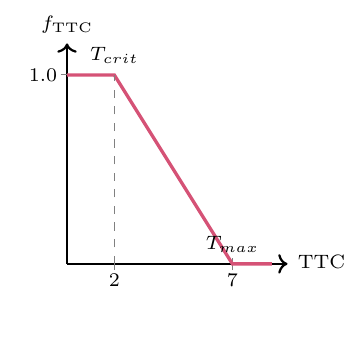
\begin{tikzpicture}
  \useasboundingbox (-0.5,-0.8) rectangle (3.2,3.0);
  \draw[->, thick] (0,0) -- (2.8,0) node[right,font=\scriptsize] {TTC (s)};
  \draw[->, thick] (0,0) -- (0,2.8) node[above,font=\scriptsize] {$f_{\text{TTC}}$};
  \node[font=\scriptsize, left] at (0,2.4) {1.0};
  \draw[gray, thin] (-0.08,2.4) -- (0.08,2.4);
  \node[font=\scriptsize, below] at (0.6,0) {2};
  \node[font=\scriptsize, below] at (2.1,0) {7};
  \draw[gray, thin] (0.6,-0.08) -- (0.6,0.08);
  \draw[gray, thin] (2.1,-0.08) -- (2.1,0.08);
  \draw[deeppink, very thick] (0,2.4) -- (0.6,2.4) -- (2.1,0) -- (2.6,0);
  \draw[gray, dashed, thin] (0.6,0) -- (0.6,2.4);
  \node[font=\scriptsize] at (0.6,2.65) {$T_{crit}$};
  \node[font=\scriptsize] at (2.1,0.25) {$T_{max}$};
\end{tikzpicture}%
}
\caption{碰撞时间因子}
\end{subfigure}
\hfill
\begin{subfigure}[b]{0.32\textwidth}
\centering
\resizebox{\textwidth}{!}{%
\begin{tikzpicture}
  \useasboundingbox (-0.5,-0.8) rectangle (3.2,3.0);
  \draw[->, thick] (0,0) -- (2.8,0) node[right,font=\scriptsize] {重叠率};
  \draw[->, thick] (0,0) -- (0,2.8) node[above,font=\scriptsize] {$f_{\text{ov}}$};
  \node[font=\scriptsize, left] at (0,2.4) {1.0};
  \draw[gray, thin] (-0.08,2.4) -- (0.08,2.4);
  \node[font=\scriptsize, below] at (2.4,0) {1.0};
  \node[font=\scriptsize, below] at (0,0) {0};
  \draw[deeppink, very thick] (0,0) -- (2.4,2.4);
\end{tikzpicture}%
}
\caption{横向重叠率因子}
\end{subfigure}
\hfill
\begin{subfigure}[b]{0.32\textwidth}
\centering
\resizebox{\textwidth}{!}{%
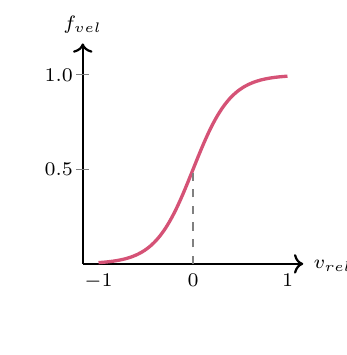
\begin{tikzpicture}
  \useasboundingbox (-0.5,-0.8) rectangle (3.2,3.0);
  % 内容居中: sigmoid 画在 [0.4, 2.8] 范围, 对称轴在 1.6
  \draw[->, thick] (0.2,0) -- (3.0,0) node[right,font=\scriptsize] {$v_{rel}/v_{max}$};
  \draw[->, thick] (0.2,0) -- (0.2,2.8) node[above,font=\scriptsize] {$f_{vel}$};
  \node[font=\scriptsize, left] at (0.2,2.4) {1.0};
  \draw[gray, thin] (0.12,2.4) -- (0.28,2.4);
  \node[font=\scriptsize, left] at (0.2,1.2) {0.5};
  \draw[gray, thin] (0.12,1.2) -- (0.28,1.2);
  % v_rel/v_max: -1 → x=0.4, 0 → x=1.6, 1 → x=2.8
  \draw[deeppink, very thick]
    plot[smooth, domain=0.4:2.8, samples=50] (\x, {2.4/(1+exp(-5*(\x-1.6)/1.2))});
  \node[font=\scriptsize, below] at (0.4,0) {$-1$};
  \node[font=\scriptsize, below] at (1.6,0) {$0$};
  \node[font=\scriptsize, below] at (2.8,0) {$1$};
  \draw[gray, dashed, thin] (1.6,0) -- (1.6,1.2);
\end{tikzpicture}%
}
\caption{相对速度因子}
\end{subfigure}

\vspace{0.8cm}

\hfill
\begin{subfigure}[b]{0.32\textwidth}
\centering
\resizebox{\textwidth}{!}{%
\begin{tikzpicture}
  \useasboundingbox (-0.5,-0.8) rectangle (3.2,3.0);
  \draw[->, thick] (0,0) -- (2.8,0);
  \draw[->, thick] (0,0) -- (0,2.8) node[above,font=\scriptsize] {$f_{\text{type}}$};
  \node[font=\scriptsize, left] at (0,2.4) {1.0};
  \draw[gray, thin] (-0.08,2.4) -- (0.08,2.4);
  \node[font=\scriptsize, left] at (0,1.68) {0.7};
  \draw[gray, thin] (-0.08,1.68) -- (0.08,1.68);
  \node[font=\scriptsize, left] at (0,0.72) {0.3};
  \draw[gray, thin] (-0.08,0.72) -- (0.08,0.72);
  \fill[dangerred!60] (0.2,0) rectangle (0.7,2.4);
  \fill[lightorange!80] (0.9,0) rectangle (1.4,1.68);
  \fill[deepblue!40] (1.6,0) rectangle (2.1,0.72);
  \node[font=\scriptsize] at (0.45,-0.35) {行人};
  \node[font=\scriptsize] at (1.15,-0.35) {车辆};
  \node[font=\scriptsize] at (1.85,-0.35) {静态};
\end{tikzpicture}%
}
\caption{障碍物类型因子}
\end{subfigure}
\hspace{0.02\textwidth}
\begin{subfigure}[b]{0.32\textwidth}
\centering
\resizebox{\textwidth}{!}{%
\begin{tikzpicture}
  \useasboundingbox (-0.5,-0.8) rectangle (3.2,3.0);
  \draw[->, thick] (0,0) -- (2.8,0) node[right,font=\scriptsize] {$d_{ij}$ (m)};
  \draw[->, thick] (0,0) -- (0,2.8) node[above,font=\scriptsize] {贡献};
  \node[font=\scriptsize, left] at (0,2.4) {1.0};
  \draw[gray, thin] (-0.08,2.4) -- (0.08,2.4);
  \node[font=\scriptsize, below] at (2.4,0) {$d_{cl}{=}10$};
  \draw[gray, thin] (2.4,-0.08) -- (2.4,0.08);
  \draw[deeppink, very thick] (0,2.4) -- (2.4,0) -- (2.7,0);
  \node[font=\scriptsize, deeppink] at (1.6,2.0) {$\frac{d_{cl}-d_{ij}}{d_{cl}}$};
\end{tikzpicture}%
}
\caption{单邻居交互贡献}
\end{subfigure}
\hfill

\caption{多因子威胁度评估的五个因子函数形态}
\label{fig:threat_factors}
\end{figure}

图\ref{fig:threat_radar}进一步给出了两个典型场景下的五维威胁度雷达图对照。左侧为对向来车场景，TTC较小、横向重叠率高、相对速度大、对象为车辆、交互密度中等，五维雷达图呈现大面积覆盖，综合威胁度接近0.85，对应$\delta_i$取到$\delta_\text{max}$附近，安全裕度最大。右侧为静止路锥场景，TTC趋于无穷、重叠率低、相对速度为零、类型权重低、密度因子接近0，雷达图呈现小面积覆盖，综合威胁度不足0.2，对应$\delta_i$接近$\delta_\text{min}$，从而大幅释放横向空间。这两张雷达图直观说明了差异化安全裕度的判别逻辑与最终数值效应。

\begin{figure}[htbp]
\centering
\begin{subfigure}[b]{0.48\textwidth}
  \centering
  \resizebox{\linewidth}{!}{% 高威胁障碍物雷达图（子图 a）
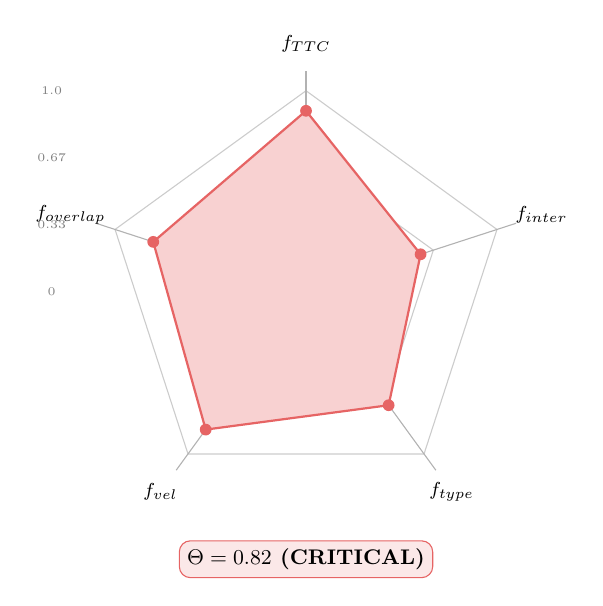
\begin{tikzpicture}[scale=0.85, transform shape]
  \foreach \r in {1, 2, 3} {
    \draw[gray!40, thin] (90:\r) \foreach \a in {162, 234, 306, 378} { -- (\a:\r) } -- cycle;
  }
  \foreach \a/\lbl in {90/$f_{TTC}$, 162/$f_{overlap}$, 234/$f_{vel}$, 306/$f_{type}$, 378/$f_{inter}$} {
    \draw[gray!60, thin] (0,0) -- (\a:3.3);
    \node[font=\footnotesize] at (\a:3.7) {\lbl};
  }

  \fill[dangerred!30, draw=dangerred, thick]
    (90:2.7) -- (162:2.4) -- (234:2.55) -- (306:2.1) -- (378:1.8) -- cycle;
  \foreach \a/\r in {90/2.7, 162/2.4, 234/2.55, 306/2.1, 378/1.8} {
    \fill[dangerred] (\a:\r) circle (2.5pt);
  }

  \node[draw=dangerred, fill=dangerred!15, rounded corners, font=\small\bfseries] at (0, -4) {$\Theta = 0.82$ (CRITICAL)};

  \node[gray, font=\tiny] at (-3.8, 0) {0};
  \node[gray, font=\tiny] at (-3.8, 1.0) {0.33};
  \node[gray, font=\tiny] at (-3.8, 2.0) {0.67};
  \node[gray, font=\tiny] at (-3.8, 3.0) {1.0};
\end{tikzpicture}
}
  \caption{高威胁 \;\; 对向来车}
  \label{fig:threat_radar:a}
\end{subfigure}\hfill
\begin{subfigure}[b]{0.48\textwidth}
  \centering
  \resizebox{\linewidth}{!}{% 低威胁障碍物雷达图（子图 b）
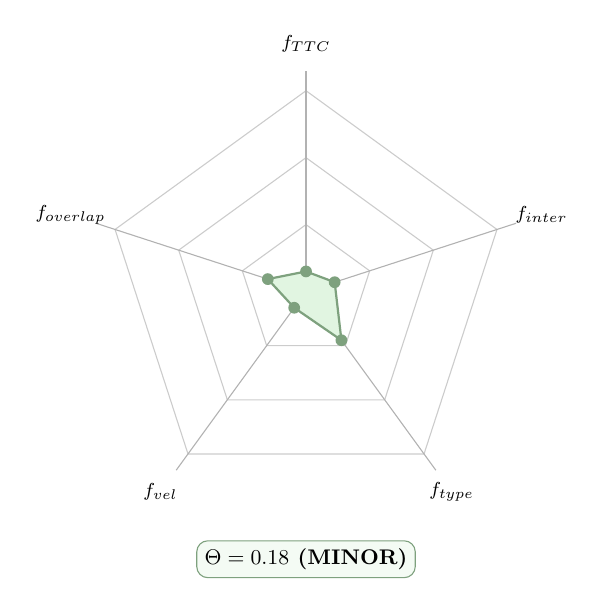
\begin{tikzpicture}[scale=0.85, transform shape]
  \foreach \r in {1, 2, 3} {
    \draw[gray!40, thin] (90:\r) \foreach \a in {162, 234, 306, 378} { -- (\a:\r) } -- cycle;
  }
  \foreach \a/\lbl in {90/$f_{TTC}$, 162/$f_{overlap}$, 234/$f_{vel}$, 306/$f_{type}$, 378/$f_{inter}$} {
    \draw[gray!60, thin] (0,0) -- (\a:3.3);
    \node[font=\footnotesize] at (\a:3.7) {\lbl};
  }

  \fill[lightgreen!40, draw=lightgreen!70!black, thick]
    (90:0.3) -- (162:0.6) -- (234:0.3) -- (306:0.9) -- (378:0.45) -- cycle;
  \foreach \a/\r in {90/0.3, 162/0.6, 234/0.3, 306/0.9, 378/0.45} {
    \fill[lightgreen!70!black] (\a:\r) circle (2.5pt);
  }

  \node[draw=lightgreen!70!black, fill=lightgreen!15, rounded corners, font=\small\bfseries] at (0, -4) {$\Theta = 0.18$ (MINOR)};
\end{tikzpicture}
}
  \caption{低威胁 \;\; 远处静态路锥}
  \label{fig:threat_radar:b}
\end{subfigure}
\caption{典型场景下的威胁度雷达图对比}
\label{fig:threat_radar}
\end{figure}

\subsection{动态安全距离}
基于综合威胁度$\Theta_i$，将式\eqref{eq:safety_margin}中的统一安全裕度替换为差异化版本

\begin{equation}
    \delta_i = \delta_{min} + (\delta_{max} - \delta_{min}) \cdot \Theta_i
    \label{eq:dynamic_delta}
\end{equation}

其中$\delta_{max} = W_{ego}/2 + d_{buf,max}$为最大安全裕度，对应CRITICAL等级障碍物，$\delta_{min} = W_{ego}/2 + d_{buf,min}$为最小安全裕度，对应MINOR等级障碍物。$d_{buf,max}$与Apollo原始\texttt{point\_extension}取值一致，$d_{buf,min}$取较小值以释放低威胁障碍物占用的横向空间，两者的具体取值由系统集成阶段的参数标定确定。

式\eqref{eq:dynamic_delta}的设计确保了以下性质。CRITICAL障碍物时$\Theta_i \to 1$，获得与Apollo原始方案相同或更大的安全裕度，不降低安全性；MINOR障碍物时$\Theta_i \to 0$，获得较小但仍安全的裕度，释放被不必要占用的横向空间。

相应地，式\eqref{eq:def_u}--\eqref{eq:def_v}中的关键量更新为差异化版本

\begin{align}
    u_i &= l_i^{-} - \delta_i \label{eq:def_u_dynamic} \\
    v_i &= l_i^{+} + \delta_i \label{eq:def_v_dynamic}
\end{align}

当$\Theta_i$对所有障碍物均取相同值时，式\eqref{eq:def_u_dynamic}--\eqref{eq:def_v_dynamic}退化为式\eqref{eq:def_u}--\eqref{eq:def_v}。动态$\delta_i$的引入不影响后续引理1和定理1的成立，两者的证明仅依赖$u$和$v$值的排序关系，只需按$u_i$而非$l_i^{-}$排序即可。

\section{本章小结}

本章针对Apollo PathBoundsDecider安全裕度一刀切的设计缺陷，提出GTOC的第一项改进，即多因子威胁度评估与差异化安全距离机制。在源码层面定位了\texttt{GetBuffer\-Between\-ADCCenter\-AndEdge}函数对所有障碍物返回相同安全距离的根源，并通过几何分析量化了统一缓冲对通行带宽度的不必要压缩。在算法设计层面，构建了融合TTC、横向重叠率、相对速度、障碍物类型与交互密度的多因子威胁度模型，并将归一化威胁度通过分段映射转化为差异化的安全裕度$\delta_i$。差异化$\delta_i$不依赖统一缓冲假设，可直接代入第六章的最大间隙公式与第七章的时空走廊边界构造，作为后续两章设计的共用输入。

\chapter{组级最优通行带与最大间隙策略}

本章对应MIKU的第二项改进，针对Apollo PathBoundsDecider对每个障碍物独立决定避让方向所导致的矛盾决策与路径BLOCKED问题，提出基于扫描线分组与最大间隙策略的组级全局最优算法。本章先分析Apollo \texttt{UpdatePathBoundary\-BySLPolygon}函数的逐障碍物贪心决策逻辑及其在两侧夹击场景下的失败模式，再构建基于纵向重叠的连通分量分组方法，在组内证明最优分割连续性引理与最大间隙最优性定理，将组合搜索复杂度从$O(2^k)$降至$O(k\log k)$。本章使用的差异化安全裕度$\delta_i$来自第四章的多因子威胁度评估，最终输出的组级避让方向决策与通行带宽度将作为第六章ST走廊边界构造的SL层基础。

\section{Apollo 逐障碍物决策的源码缺陷与失败模式}
\label{sec:problem_sl}

\subsection{源码逻辑与决策入口}

PathBoundsDecider是Apollo路径规划阶段的关键模块，负责在每个离散纵向位置$s$处构建横向路径边界$[l^-(s),\; l^+(s)]$。问题在于它对每个障碍物独立地决定避让方向（LEFT\_NUDGE或RIGHT\_NUDGE），而不考虑同一$s$截面上其他活跃障碍物的存在。当道路两侧同时存在障碍物时，这种逐障碍物的贪心决策可能产生相互矛盾的避让方向，即左侧障碍物使上边界下压、右侧障碍物使下边界上抬，导致$l^+(s) < l^-(s)$，路径边界被判定为BLOCKED，最终触发FallbackPath停车。

问题根源在\texttt{UpdatePathBoundary\-BySLPolygon}函数，其逻辑分三步：逐障碍物独立决定避让方向、根据避让方向收缩路径边界、检测边界交叉并截断路径。代码\ref{lst:update_path_boundary}展示了该函数的关键流程。

\begin{lstlisting}[language=C++,caption={UpdatePathBoundaryBySLPolygon核心逻辑},label={lst:update_path_boundary}]
// path_bounds_decider_util.cc: UpdatePathBoundaryBySLPolygon
for (size_t i = 1; i < path_boundary->size(); ++i) {
  auto& left_bound = path_boundary->at(i).l_upper;   // 上边界
  auto& right_bound = path_boundary->at(i).l_lower;  // 下边界
  for (size_t j = 0; j < sl_polygon->size(); j++) {
    // --- 步骤1: 逐障碍物独立决定避让方向 ---
    if (sl_polygon->at(j).NudgeInfo() == SLPolygon::UNDEFINED) {
      double obs_l = (l_lower + l_upper) / 2;  // 障碍物中心横向位置
      if (is_passable_right && is_passable_left) {
        // 两侧均可通行时，根据障碍物中心与参考线的相对位置决定
        if (last_max_nudge_l < obs_l) {
          sl_polygon->at(j).SetNudgeInfo(SLPolygon::RIGHT_NUDGE);
        } else {
          sl_polygon->at(j).SetNudgeInfo(SLPolygon::LEFT_NUDGE);
        }
      } else if (is_passable_right) {
        sl_polygon->at(j).SetNudgeInfo(SLPolygon::RIGHT_NUDGE);
      } else {
        sl_polygon->at(j).SetNudgeInfo(SLPolygon::LEFT_NUDGE);
      }
    }
    // --- 步骤2: 根据避让方向更新边界 ---
    if (sl_polygon->at(j).NudgeInfo() == SLPolygon::RIGHT_NUDGE) {
      if (!sl_polygon->at(j).is_passable()[RIGHT_INDEX]) {
        sl_polygon->at(j).SetNudgeInfo(SLPolygon::BLOCKED);
        break;  // 右侧不可通行，标记BLOCKED
      }
      // 上边界收缩至障碍物左边缘减安全距离
      if (obs_right_nudge_bound.l_upper.l < left_bound.l) {
        left_bound.l = obs_right_nudge_bound.l_upper.l;
        left_bound.type = BoundType::OBSTACLE;
      }
    } else if (sl_polygon->at(j).NudgeInfo() == SLPolygon::LEFT_NUDGE) {
      if (!sl_polygon->at(j).is_passable()[LEFT_INDEX]) {
        sl_polygon->at(j).SetNudgeInfo(SLPolygon::BLOCKED);
        break;  // 左侧不可通行，标记BLOCKED
      }
      // 下边界上抬至障碍物右边缘加安全距离
      if (obs_left_nudge_bound.l_lower.l > right_bound.l) {
        right_bound.l = obs_left_nudge_bound.l_lower.l;
        right_bound.type = BoundType::OBSTACLE;
      }
    }
  }
  // --- 步骤3: BLOCKED判定与路径截断 ---
  if (!blocked_id->empty()) {
    TrimPathBounds(i, path_boundary);  // 截断后续路径边界
    return false;                      // 触发FallbackPath停车
  }
}
\end{lstlisting}

步骤1对每个在位置$s$处活跃的障碍物，通过\texttt{SetNudgeInfo}函数根据障碍物中心相对于参考线的横向位置独立决定\texttt{RIGHT\_NUDGE}即从右侧绕行使上边界下压，或\texttt{LEFT\_NUDGE}即从左侧绕行使下边界上抬。步骤2根据避让方向对路径边界进行收缩，安全距离\texttt{delta}由自车半宽即\texttt{GetBufferBetweenADCCenterAndEdge}的返回值与额外缓冲参数\texttt{obstacle\_lat\_buffer}相加得到。步骤3在上下边界交叉即存在BLOCKED标记的障碍物时，调用\texttt{TrimPathBounds}清除后续路径边界并返回\texttt{false}，最终触发\texttt{FallbackPath}生成减速停车轨迹。

\subsection{独立决策的失败模式}

以下通过一个对称场景说明独立决策如何导致不必要的停车。

\textbf{场景设定}\quad 双车道道路总宽7.5\,m，$l_{road}^- = -3.75$\,m，$l_{road}^+ = 3.75$\,m。在某纵向位置$s^*$处同时存在两个路锥，关于参考线近似对称

\begin{itemize}[noitemsep]
\item $O_a$偏右，横向占据$[0.1,\; 0.4]$\,m，中心$0.25$\,m
\item $O_b$偏左，横向占据$[-0.4,\; -0.1]$\,m，中心$-0.25$\,m
\end{itemize}

两个路锥均未越过车道中线，安全距离$\delta = 1.2$\,m。

\textbf{Apollo独立决策}\quad $O_a$中心$0.25 > 0$，分配RIGHT\_NUDGE，上边界收缩至
\[
l^+(s^*) = 0.1 - 1.2 = -1.1\,\text{m}
\]
$O_b$中心$-0.25 < 0$，分配LEFT\_NUDGE，下边界抬升至
\[
l^-(s^*) = -0.1 + 1.2 = 1.1\,\text{m}
\]
$l^+ = -1.1 < l^- = 1.1$，判定BLOCKED。贪心策略将自车挤入两个路锥之间仅0.2\,m的间隙，路径不可行，触发停车。

\textbf{全局统一决策}\quad 将两个路锥作为一组，统一分配RIGHT\_NUDGE，自车从两者右侧绕行
\[
l^+(s^*) = \min(0.1 - 1.2,\; -0.4 - 1.2) = -1.6\,\text{m}, \quad l^-(s^*) = -3.75\,\text{m}
\]
通行带宽度$W = -1.6 - (-3.75) = 2.15$\,m，自车可借用相邻车道从右侧安全通过。由对称性，统一LEFT\_NUDGE同样可行，$W = 3.75 - 1.6 = 2.15$\,m。

贪心策略将两个偏向不同侧的障碍物分别向内挤压，全局协调只需统一绕行方向，即可利用道路另一侧的充裕空间。当$k$个障碍物在同一纵向位置活跃时，避让方向共有$2^k$种组合，贪心策略只检查了其中一种，可能恰好选中不可行的组合而遗漏可行解。该问题的形式化建模在第三章统一框架下已经给出，高效求解方法将在本章下一节详细展开。

图\ref{fig:path_conservative}展示了该场景中独立决策与全局协调的对比。

\begin{figure}[htbp]
\centering
\begin{subfigure}[b]{0.48\textwidth}
  \centering
  \resizebox{\linewidth}{!}{% 子图(a)：独立决策，矛盾避让 → BLOCKED
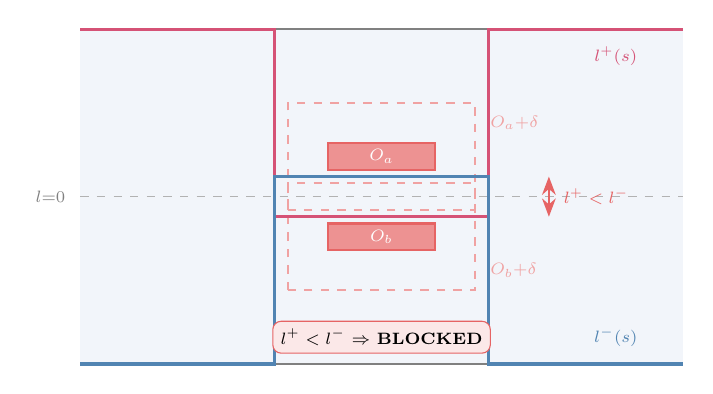
\begin{tikzpicture}[scale=0.85, transform shape]
  % 道路背景
  \fill[bglight] (-0.5,-2.5) rectangle (8.5,2.5);
  \draw[gray, thick] (-0.5, 2.5) -- (8.5, 2.5);
  \draw[gray, thick] (-0.5,-2.5) -- (8.5,-2.5);
  \draw[dashed, gray!60] (-0.5, 0) -- (8.5, 0);
  \node[gray, font=\scriptsize, anchor=east] at (-0.6, 0) {$l{=}0$};

  % O_a（上方）
  \fill[dangerred!70, draw=dangerred, thick] (3.2, 0.4) rectangle (4.8, 0.8);
  \node[font=\scriptsize, white] at (4.0, 0.6) {$O_a$};

  % O_b（下方）
  \fill[dangerred!70, draw=dangerred, thick] (3.2,-0.8) rectangle (4.8,-0.4);
  \node[font=\scriptsize, white] at (4.0,-0.6) {$O_b$};

  % 膨胀虚线 δ=0.6
  \draw[dangerred!60, dashed, thick] (2.6,-0.2) rectangle (5.4, 1.4);
  \node[dangerred!60, font=\scriptsize, anchor=west] at (5.5, 1.1) {$O_a{+}\delta$};
  \draw[dangerred!60, dashed, thick] (2.6,-1.4) rectangle (5.4, 0.2);
  \node[dangerred!60, font=\scriptsize, anchor=west] at (5.5,-1.1) {$O_b{+}\delta$};

  % 上界 l+(s)：右绕 O_a
  \draw[deeppink, very thick]
    (-0.5, 2.5) -- (2.4, 2.5) -- (2.4, -0.3) -- (5.6, -0.3) -- (5.6, 2.5) -- (8.5, 2.5);
  \node[deeppink, font=\scriptsize] at (7.5, 2.1) {$l^+(s)$};

  % 下界 l-(s)：左绕 O_b
  \draw[deepblue, very thick]
    (-0.5,-2.5) -- (2.4,-2.5) -- (2.4, 0.3) -- (5.6, 0.3) -- (5.6,-2.5) -- (8.5,-2.5);
  \node[deepblue, font=\scriptsize] at (7.5,-2.1) {$l^-(s)$};

  % 矛盾标注
  \draw[dangerred, thick, {Stealth}-{Stealth}] (6.5,-0.3) -- (6.5, 0.3);
  \node[dangerred, font=\scriptsize, anchor=west] at (6.6, 0) {$l^+ < l^-$};

  % BLOCKED 判定
  \node[draw=dangerred, fill=dangerred!15, font=\scriptsize,
        rounded corners=3pt, align=center] at (4.0,-2.1)
    {$l^+ < l^-$ $\Rightarrow$ \textbf{BLOCKED}};
\end{tikzpicture}
}
  \caption{独立决策，矛盾避让 $\to$ BLOCKED}
  \label{fig:path_conservative:a}
\end{subfigure}\hfill
\begin{subfigure}[b]{0.48\textwidth}
  \centering
  \resizebox{\linewidth}{!}{% 子图(b)：全局协调，统一右绕 → 通行
\begin{tikzpicture}[scale=0.85, transform shape]
  % 道路背景
  \fill[bglight] (-0.5,-2.5) rectangle (8.5,2.5);
  \draw[gray, thick] (-0.5, 2.5) -- (8.5, 2.5);
  \draw[gray, thick] (-0.5,-2.5) -- (8.5,-2.5);
  \draw[dashed, gray!60] (-0.5, 0) -- (8.5, 0);
  \node[gray, font=\scriptsize, anchor=east] at (-0.6, 0) {$l{=}0$};

  % O_a（上方）
  \fill[dangerred!70, draw=dangerred, thick] (3.2, 0.4) rectangle (4.8, 0.8);
  \node[font=\scriptsize, white] at (4.0, 0.6) {$O_a$};

  % O_b（下方）
  \fill[dangerred!70, draw=dangerred, thick] (3.2,-0.8) rectangle (4.8,-0.4);
  \node[font=\scriptsize, white] at (4.0,-0.6) {$O_b$};

  % 膨胀虚线 δ=0.6
  \draw[dangerred!60, dashed, thick] (2.6,-0.2) rectangle (5.4, 1.4);
  \node[dangerred!60, font=\scriptsize, anchor=west] at (5.5, 0.6) {$O_a{+}\delta$};
  \draw[dangerred!60, dashed, thick] (2.6,-1.4) rectangle (5.4, 0.2);
  \node[dangerred!60, font=\scriptsize, anchor=west] at (5.5,-0.6) {$O_b{+}\delta$};

  % 上界 l+(s)：统一右绕，压到 O_b 膨胀下缘
  \draw[deeppink, very thick]
    (-0.5, 2.5) -- (2.4, 2.5) -- (2.4, -1.5) -- (5.6, -1.5) -- (5.6, 2.5) -- (8.5, 2.5);
  \node[deeppink, font=\scriptsize] at (7.5, 2.1) {$l^+(s)$};

  % 下界 l-(s)：道路下界
  \draw[deepblue, very thick, dashed]
    (-0.5,-2.5) -- (8.5,-2.5);
  \node[deepblue, font=\scriptsize, left] at (-0.6,-2.5) {$l^-(s)$};

  % 通行带
  \fill[lightgreen, opacity=0.25] (-0.5,-2.5) rectangle (8.5,-1.5);

  % 通行带宽度标注
  \draw[deeppink, thick, {Stealth}-{Stealth}] (0.5,-2.5) -- (0.5,-1.5);
  \node[deeppink, font=\scriptsize, anchor=east] at (0.4,-2.0) {$W{=}1.0$m};

  % 自车轨迹
  \draw[deepblue, very thick, -{Stealth}]
    plot[smooth, tension=0.55] coordinates
      {(0.5, 0) (1.5,-0.5) (2.5,-1.8) (4.0,-2.0) (5.5,-1.8) (6.5,-0.5) (7.5, 0)};
  \node[deepblue, font=\scriptsize] at (4.0,-2.45) {规划轨迹};

  % PASS 判定
  \node[draw=lightgreen!80!black, fill=lightgreen!20, font=\scriptsize,
        rounded corners=3pt, align=center] at (4.0, 2.0)
    {统一右绕 $\Rightarrow$ \textbf{PASS}};
\end{tikzpicture}
}
  \caption{全局协调，统一右绕 $\to$ 通行}
  \label{fig:path_conservative:b}
\end{subfigure}
\caption{独立决策导致矛盾避让方向与全局协调的对比}
\label{fig:path_conservative}
\end{figure}

除了两个障碍物的极端情形外，随着障碍物数量增加，独立决策导致的可行域压缩会以近似指数方式恶化。图\ref{fig:feasible_compress}给出了同一车道内从2个、4个到极端密度障碍物场景下的可行域演化。2个障碍物场景下，尚存较宽的可行通带可供自车选择，尽管贪心决策已开始压缩通带宽度；4个障碍物场景下，多次独立收缩使可行域退化为断续的狭窄通带，任一处出现贪心矛盾即触发BLOCKED；极端密度场景下，可行域进一步碎片化，几乎任何贪心决策组合都会导致某处边界失效。可见在高密度场景下，改进决策粒度对可行性恢复的贡献度远高于单纯调整安全裕度。

\begin{figure}[htbp]
\centering
\begin{subfigure}[b]{0.32\textwidth}
  \centering
  \resizebox{\linewidth}{!}{% 2 个障碍物 通行带可行（子图 a）
\begin{tikzpicture}[scale=0.7, transform shape]
  \draw[-Stealth, thick] (0,-2.5) -- (8.5,-2.5) node[right, font=\footnotesize] {$s$};
  \draw[-Stealth, thick] (0,-2.5) -- (0,2.5) node[above, font=\footnotesize] {$l$};

  \draw[gray, thick] (0,1.875) -- (8,1.875);
  \draw[gray, thick] (0,-1.875) -- (8,-1.875);
  \draw[gray, dashed] (0,0) -- (8,0);

  \begin{scope}[on background layer]
    \fill[bglight] (0,-1.875) rectangle (8,1.875);
  \end{scope}

  % O1（上方靠边）y=[0.6, 1.3], s=[2, 4]
  \fill[dangerred!70, draw=dangerred, thick] (2,0.6) rectangle (4,1.3);
  \node[white, font=\footnotesize\bfseries] at (3,0.95) {$O_1$};

  % O2（下方靠边）y=[-1.2, -0.5], s=[5, 7]
  \fill[dangerred!70, draw=dangerred, thick] (5,-1.2) rectangle (7,-0.5);
  \node[white, font=\footnotesize\bfseries] at (6,-0.85) {$O_2$};

  % O1 右绕 → 上界压到 O1 膨胀下缘 (0.6-0.4=0.2)
  \draw[deeppink, very thick]
    (0,1.875) -- (1.8,1.875) -- (1.8,0.2) -- (4.2,0.2) -- (4.2,1.875) -- (8,1.875);
  \node[deeppink, font=\tiny] at (1, 2.1) {$l^+(s)$};

  % O2 左绕 → 下界抬到 O2 膨胀上缘 (-0.5+0.4=-0.1)
  \draw[deepblue, very thick]
    (0,-1.875) -- (4.8,-1.875) -- (4.8,-0.1) -- (7.2,-0.1) -- (7.2,-1.875) -- (8,-1.875);
  \node[deepblue, font=\tiny] at (7.5, -2.1) {$l^-(s)$};

  \node[lightgreen!60!black, font=\footnotesize\bfseries] at (4,-1.35) {通行带充足};
\end{tikzpicture}
}
  \caption{2 个障碍物}
  \label{fig:feasible_compress:a}
\end{subfigure}\hfill
\begin{subfigure}[b]{0.32\textwidth}
  \centering
  \resizebox{\linewidth}{!}{% 4 个障碍物 通行带狭窄（子图 b）
\begin{tikzpicture}[scale=0.7, transform shape]
  \draw[-Stealth, thick] (0,-2.5) -- (8.5,-2.5) node[right, font=\footnotesize] {$s$};
  \draw[-Stealth, thick] (0,-2.5) -- (0,2.5) node[above, font=\footnotesize] {$l$};

  \draw[gray, thick] (0,1.875) -- (8,1.875);
  \draw[gray, thick] (0,-1.875) -- (8,-1.875);
  \draw[gray, dashed] (0,0) -- (8,0);

  \begin{scope}[on background layer]
    \fill[bglight] (0,-1.875) rectangle (8,1.875);
  \end{scope}

  % O1（上方靠边）y=[0.5, 1.1], s=[1, 2.5]
  \fill[dangerred!70, draw=dangerred, thick] (1,0.5) rectangle (2.5,1.1);
  \node[white, font=\tiny\bfseries] at (1.75,0.8) {$O_1$};

  % O2（下方靠边）y=[-1.0, -0.4], s=[2.5, 4]
  \fill[dangerred!70, draw=dangerred, thick] (2.5,-1.0) rectangle (4,-0.4);
  \node[white, font=\tiny\bfseries] at (3.25,-0.7) {$O_2$};

  % O3（上方靠边）y=[0.4, 0.9], s=[4.5, 6]
  \fill[dangerred!70, draw=dangerred, thick] (4.5,0.4) rectangle (6,0.9);
  \node[white, font=\tiny\bfseries] at (5.25,0.65) {$O_3$};

  % O4（下方靠边）y=[-0.8, -0.2], s=[6, 7.5]
  \fill[dangerred!70, draw=dangerred, thick] (6,-0.8) rectangle (7.5,-0.2);
  \node[white, font=\tiny\bfseries] at (6.75,-0.5) {$O_4$};

  % 上界 l+(s)：O1右绕压到0.1, O3右绕压到0.0
  \draw[deeppink, very thick]
    (0,1.875) -- (0.8,1.875) -- (0.8,0.1) -- (2.7,0.1)
    -- (2.7,1.875) -- (4.3,1.875) -- (4.3,0.0) -- (6.2,0.0)
    -- (6.2,1.875) -- (8,1.875);

  % 下界 l-(s)：O2左绕抬到0.0, O4左绕抬到0.2
  \draw[deepblue, very thick]
    (0,-1.875) -- (2.3,-1.875) -- (2.3,0.0) -- (4.2,0.0)
    -- (4.2,-1.875) -- (5.8,-1.875) -- (5.8,0.2) -- (7.7,0.2)
    -- (7.7,-1.875) -- (8,-1.875);

  % 窄处标注
  \draw[lightorange, ultra thick] (2.5,0.0) -- (2.5,0.1);
  \node[lightorange!80!black, font=\tiny\bfseries, anchor=west] at (2.6,0.05) {窄};
  \draw[lightorange, ultra thick] (6,0.0) -- (6,0.2);
  \node[lightorange!80!black, font=\tiny\bfseries, anchor=west] at (6.1,0.1) {窄};

  \node[deeppink, font=\tiny] at (0.5, 2.1) {$l^+(s)$};
  \node[deepblue, font=\tiny] at (7.5, -2.1) {$l^-(s)$};
  \node[lightorange!80!black, font=\footnotesize\bfseries] at (4,-1.5) {多次收缩 通行带退化};
\end{tikzpicture}
}
  \caption{4 个障碍物}
  \label{fig:feasible_compress:b}
\end{subfigure}\hfill
\begin{subfigure}[b]{0.32\textwidth}
  \centering
  \resizebox{\linewidth}{!}{% 密集障碍物 BLOCKED（子图 c）
\begin{tikzpicture}[scale=0.7, transform shape]
  \draw[-Stealth, thick] (0,-2.5) -- (8.5,-2.5) node[right, font=\footnotesize] {$s$};
  \draw[-Stealth, thick] (0,-2.5) -- (0,2.5) node[above, font=\footnotesize] {$l$};

  \draw[gray, thick] (0,1.875) -- (8,1.875);
  \draw[gray, thick] (0,-1.875) -- (8,-1.875);
  \draw[gray, dashed] (0,0) -- (8,0);

  \begin{scope}[on background layer]
    \fill[bglight] (0,-1.875) rectangle (8,1.875);
  \end{scope}

  % 密集障碍物（交替上下，靠近道路边缘）
  \fill[dangerred!70, draw=dangerred, thick] (0.5,0.4) rectangle (1.5,1.2);
  \node[white, font=\tiny\bfseries] at (1,0.8) {$O_1$};

  \fill[dangerred!70, draw=dangerred, thick] (1.5,-1.1) rectangle (2.5,-0.3);
  \node[white, font=\tiny\bfseries] at (2,-0.7) {$O_2$};

  \fill[dangerred!70, draw=dangerred, thick] (2.5,0.3) rectangle (3.5,1.1);
  \node[white, font=\tiny\bfseries] at (3,0.7) {$O_3$};

  \fill[dangerred!70, draw=dangerred, thick] (3.5,-1.0) rectangle (4.5,-0.2);
  \node[white, font=\tiny\bfseries] at (4,-0.6) {$O_4$};

  \fill[dangerred!70, draw=dangerred, thick] (4.5,0.5) rectangle (5.5,1.3);
  \node[white, font=\tiny\bfseries] at (5,0.9) {$O_5$};

  \fill[dangerred!70, draw=dangerred, thick] (5.5,-1.2) rectangle (6.5,-0.3);
  \node[white, font=\tiny\bfseries] at (6,-0.75) {$O_6$};

  \fill[dangerred!70, draw=dangerred, thick] (6.5,0.3) rectangle (7.5,1.1);
  \node[white, font=\tiny\bfseries] at (7,0.7) {$O_7$};

  % 上界 l+(s)：逐步压低 (δ=0.4)
  \draw[deeppink, very thick]
    (0,1.875) -- (0.3,1.875) -- (0.3,0.0) -- (1.7,0.0)
    -- (1.7,1.875) -- (2.3,1.875) -- (2.3,-0.1) -- (3.7,-0.1)
    -- (3.7,1.875) -- (4.3,1.875) -- (4.3,0.1) -- (5.7,0.1);

  % 下界 l-(s)：逐步抬高
  \draw[deepblue, very thick]
    (0,-1.875) -- (1.3,-1.875) -- (1.3,0.1) -- (2.7,0.1)
    -- (2.7,-1.875) -- (3.3,-1.875) -- (3.3,0.2) -- (4.7,0.2);

  % BLOCKED 点
  \fill[dangerred] (4.5,0.15) circle (3pt);

  % 截断区域
  \fill[dangerred, opacity=0.1] (4.5,-1.875) rectangle (8,1.875);
  \node[dangerred, font=\footnotesize\bfseries] at (6.5,1.3) {$l^+ < l^- \rightarrow$ BLOCKED};
  \node[dangerred, font=\tiny] at (6.5,-1.5) {TrimPathBounds 截断};

  \node[deeppink, font=\tiny] at (0.5, 2.1) {$l^+(s)$};
  \node[deepblue, font=\tiny] at (0.5, -2.1) {$l^-(s)$};
\end{tikzpicture}
}
  \caption{密集障碍物}
  \label{fig:feasible_compress:c}
\end{subfigure}
\caption{多障碍物场景下可行域的退化演化}
\label{fig:feasible_compress}
\end{figure}

\subsection{BLOCKED 后的截断与恢复机制局限}

当PathBoundsDecider判定BLOCKED后，调用\texttt{TrimPathBounds}截断路径

\begin{lstlisting}[language=C++,caption={TrimPathBounds路径截断},label={lst:trim_path}]
// path_bounds_decider_util.cc: TrimPathBounds
void PathBoundsDeciderUtil::TrimPathBounds(
    const int path_blocked_idx, PathBoundary* const path_boundaries) {
  if (path_blocked_idx != -1) {
    if (path_blocked_idx == 0) {
      AINFO << "Completely blocked. Cannot move at all.";
    }
    double front_edge_to_center =
        VehicleConfigHelper::GetConfig().vehicle_param().front_edge_to_center();
    double trimmed_s =
        path_boundaries->at(path_blocked_idx).s - front_edge_to_center;
    while (path_boundaries->size() > 1 &&
           path_boundaries->back().s > trimmed_s) {
      path_boundaries->pop_back();  // 逐个弹出BLOCKED位置之后的边界点
    }
  }
}
\end{lstlisting}

该函数将路径边界截断至BLOCKED位置的前方即减去车头到中心的距离，后续\texttt{FallbackPath}模块基于截断后的短路径生成减速停车轨迹。一旦某个避让方向组合导致BLOCKED，系统不会回溯尝试其他方向组合，而是直接进入停车流程。

Apollo提供的\texttt{LaneBorrowPath}机制可以在一定条件下缓解BLOCKED问题，但该机制的触发条件非常严格。代码\ref{lst:lane_borrow_conditions}展示了借道决策需要通过的5个前置检查及条件4的具体实现

\begin{lstlisting}[language=C++,caption={LaneBorrowPath的前置条件与长期阻塞判定},label={lst:lane_borrow_conditions}]
// lane_borrow_path.cc: IsNecessaryToBorrowLane
// 条件1: 仅单参考线场景（路口等多参考线场景不借道）
if (!HasSingleReferenceLine(*frame_)) { return false; }
// 条件2: 自车速度低于阈值（默认5.0 m/s）
if (!IsWithinSidePassingSpeedADC(*frame_)) { return false; }
// 条件3: 阻塞障碍物远离路口
if (!IsBlockingObstacleFarFromIntersection(*ref_info)) { return false; }
// 条件4: 障碍物持续阻塞达到cycle阈值（默认3个周期）
if (!IsLongTermBlockingObstacle()) { return false; }
// 条件5: 阻塞障碍物在目的地范围内
if (!IsBlockingObstacleWithinDestination(*ref_info)) { return false; }

// 条件4的具体实现: IsLongTermBlockingObstacle
bool LaneBorrowPath::IsLongTermBlockingObstacle() {
  if (injector_->planning_context()->planning_status().path_decider()
          .front_static_obstacle_cycle_counter() >=
      config_.long_term_blocking_obstacle_cycle_threshold()) {  // 默认值: 3
    return true;
  }
  return false;
}
\end{lstlisting}

即使存在可行的借道方案，系统也必须先经历至少3个规划周期约300\,ms的停车等待才会尝试借道，且借道仅在单参考线、低速、远离路口等条件同时满足时才被允许。在路口附近、高速行驶或多参考线场景下，LaneBorrow机制不会触发，BLOCKED判定将直接导致停车。
\section{纵向重叠分组与连通分量}
\label{sec:grouping_connected}
本节起所有$u_i$和$v_i$均使用式\eqref{eq:def_u_dynamic}--\eqref{eq:def_v_dynamic}中的动态安全距离$\delta_i$计算，后续引理和定理的证明不依赖$\delta$是否为常数，仅依赖$u$和$v$值的排序性。
在全路径范围内，不同纵向位置$s$处的活跃障碍物集合不同，因此式\eqref{eq:joint_opt}的优化不能在单一截面上完成。关键观察是，如果两组障碍物在纵向上完全不重叠，则它们的避让决策相互独立。

定义纵向重叠关系。两个障碍物$O_i$和$O_j$纵向重叠，当且仅当它们的纵向区间有交集

\begin{equation}
    O_i \sim O_j \iff [s_i^{-}, s_i^{+}] \cap [s_j^{-}, s_j^{+}] \neq \emptyset
    \label{eq:overlap_relation}
\end{equation}

该重叠关系是对称的但不具有传递性。取其传递闭包，即存在一系列中间障碍物依次纵向重叠，将$n$个障碍物划分为$m$个连通分量$C_1, C_2, \ldots, C_m$。同一连通分量内的障碍物通过重叠链相连，不同连通分量之间在纵向上完全分离。由于不同连通分量在纵向上不重叠，其避让决策互不影响，可以独立求解。

连通分量的检测采用扫描线算法，将所有障碍物按$s_i^{-}$升序排列，维护一个变量$s_{max}$记录当前连通分量中所有障碍物的最大$s^{+}$值。扫描过程中，若下一个障碍物的$s^{-}$不超过$s_{max}$，则将其归入当前分量并更新$s_{max}$；否则开始新的分量。该过程的时间复杂度为$O(n \log n)$其中排序占主导，扫描本身仅需$O(n)$。

纵向上彼此重叠的障碍物需要在同一个横向截面上协调决策，因此必须归为同一组；纵向上完全分离的障碍物组，自车在通过一组时尚未遇到下一组，决策互不影响。问题因此天然分解为多个独立子问题，这是算法高效性的基础。图\ref{fig:scanline_grouping}以六障碍物算例展示了扫描过程，$s_{max}$扫描线沿$s$轴从左到右推进，遇到与当前组重叠的障碍物即并入，否则切出新分量，最终得到三个互不重叠的连通分量$C_1$到$C_3$。

\begin{figure}[htbp]
\centering
\resizebox{\textwidth}{!}{% 扫描线按 s_i^- 升序合并连通分量的过程
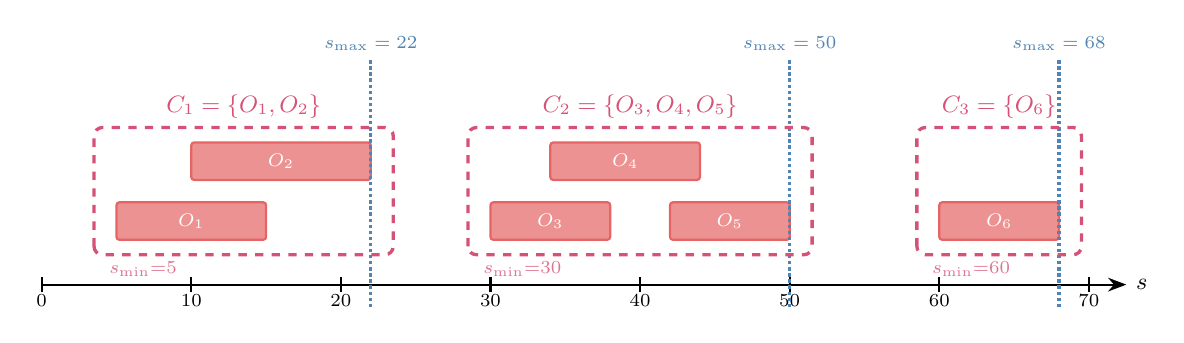
\begin{tikzpicture}[scale=0.95, transform shape,
    obs/.style={fill=dangerred!70, draw=dangerred, thick, rounded corners=1pt},
    grp/.style={draw=deeppink, very thick, dashed, rounded corners=3pt},
]

% s 轴
\draw[-Stealth, thick] (0,0) -- (14.5,0) node[right, font=\small] {$s$};
\foreach \x/\lab in {0/0, 2/10, 4/20, 6/30, 8/40, 10/50, 12/60, 14/70}
    \draw[thick] (\x,-0.1) -- (\x,0.1) node[below=0.1cm, font=\scriptsize] {\lab};

% 六个障碍物的 [s^-, s^+] 区间（按 s^- 升序）
% O1: [5, 15]  O2: [10, 22]  O3: [30, 38]  O4: [34, 44]  O5: [42, 50]  O6: [60, 68]
\fill[obs] (1,0.6) rectangle (3,1.1);
\node[white, font=\scriptsize\bfseries] at (2,0.85) {$O_1$};

\fill[obs] (2,1.4) rectangle (4.4,1.9);
\node[white, font=\scriptsize\bfseries] at (3.2,1.65) {$O_2$};

\fill[obs] (6,0.6) rectangle (7.6,1.1);
\node[white, font=\scriptsize\bfseries] at (6.8,0.85) {$O_3$};

\fill[obs] (6.8,1.4) rectangle (8.8,1.9);
\node[white, font=\scriptsize\bfseries] at (7.8,1.65) {$O_4$};

\fill[obs] (8.4,0.6) rectangle (10,1.1);
\node[white, font=\scriptsize\bfseries] at (9.2,0.85) {$O_5$};

\fill[obs] (12,0.6) rectangle (13.6,1.1);
\node[white, font=\scriptsize\bfseries] at (12.8,0.85) {$O_6$};

% s_max 扫描线（当前最大上界）
\draw[deepblue, very thick, densely dotted] (4.4,-0.3) -- (4.4,3.0);
\node[deepblue, font=\scriptsize, anchor=south] at (4.4,3.0) {$s_{\max}=22$};

\draw[deepblue, very thick, densely dotted] (10,-0.3) -- (10,3.0);
\node[deepblue, font=\scriptsize, anchor=south] at (10,3.0) {$s_{\max}=50$};

\draw[deepblue, very thick, densely dotted] (13.6,-0.3) -- (13.6,3.0);
\node[deepblue, font=\scriptsize, anchor=south] at (13.6,3.0) {$s_{\max}=68$};

% 三个连通分量分组框
\draw[grp] (0.7,0.4) rectangle (4.7,2.1);
\node[deeppink, font=\small\bfseries, anchor=south] at (2.7,2.1) {$C_1=\{O_1,O_2\}$};
\node[deeppink!80, font=\scriptsize, anchor=north west] at (0.78,0.43) {$s_{\min}{=}5$};

\draw[grp] (5.7,0.4) rectangle (10.3,2.1);
\node[deeppink, font=\small\bfseries, anchor=south] at (8,2.1) {$C_2=\{O_3,O_4,O_5\}$};
\node[deeppink!80, font=\scriptsize, anchor=north west] at (5.78,0.43) {$s_{\min}{=}30$};

\draw[grp] (11.7,0.4) rectangle (13.9,2.1);
\node[deeppink, font=\small\bfseries, anchor=south] at (12.8,2.1) {$C_3=\{O_6\}$};
\node[deeppink!80, font=\scriptsize, anchor=north west] at (11.78,0.43) {$s_{\min}{=}60$};

\end{tikzpicture}
}
\caption{扫描线算法按$s_i^-$升序合并连通分量的过程}
\label{fig:scanline_grouping}
\end{figure}

当障碍物仅在纵向上部分重叠即存在某些$s$截面上只有部分障碍物活跃时，组内处理采用保守近似，以所有障碍物均同时活跃为假设计算间隙。这可能导致轻微的次优性，但算法的正确性可由以下两步论证保证。首先，在最密集截面上按定理1选定的分割点$p^{*}$将障碍物划分为左绕集合$\mathcal{L}_{p^{*}}$和右绕集合$\mathcal{R}_{p^{*}}$，此时通行带上下界由$l^{+} = \min_{i \in \mathcal{R}_{p^{*}}} u_i$和$l^{-} = \max_{i \in \mathcal{L}_{p^{*}}} v_i$给出。其次，任意稀疏截面对应的活跃障碍物集合均为最密集截面的子集，移除部分障碍物只会使$\min$运算作用于更大的集合从而放宽$l^{+}$的上界，同时使$\max$运算作用于更大的集合从而放宽$l^{-}$的下界。若$\mathcal{L}_{p^{*}}$或$\mathcal{R}_{p^{*}}$被移空，则相应方向退化为道路边界。因此通行带宽度$W = l^{+} - l^{-}$单调不减，最密集截面上的决策在所有稀疏截面上均保持可行，且通行带不会更窄。

全路径的最小通行带宽度由最窄的连通分量决定，即木桶效应

\begin{equation}
    W^{*} = \min_{j=1,\ldots,m} W^{*}(C_j)
    \label{eq:global_width}
\end{equation}

下面聚焦于单个连通分量的最优求解。设该分量内有$k$个障碍物，在其公共$s$截面上按$u_i$值升序排列为$O_{(1)}, O_{(2)}, \ldots, O_{(k)}$，使得$u_{(1)} \leq u_{(2)} \leq \cdots \leq u_{(k)}$。按$u_i$排序而非$l_i^{-}$排序的原因在于引入动态安全距离$\delta_i$后，$u_i = l_i^{-} - \delta_i$的排序可能不再与$l_i^{-}$一致，详见\S\ref{sec:dynamic_delta_synthesis}，而后续引理和定理的证明仅依赖$u$值的排序性。问题转化为在$k$个按$u_i$排列的障碍物上，如何分配左绕/右绕决策以最大化通行带宽度。

从几何直觉看，$k$个按横向位置排列的障碍物将车道的横向空间分割为$k+1$个通道，包括最右侧障碍物与道路右边界之间、相邻障碍物之间、以及最左侧障碍物与道路左边界之间的间隙。最优策略是选择其中最宽的通道通行，通道一侧的所有障碍物划归左绕、另一侧的划归右绕，形成一个在排序中连续的分割。搜索空间从$2^k$个任意分配降为$k+1$个候选通道的选取。以下引理和定理给出严格证明，并建立通行带宽度与间隙之间的精确等式。

\section{最优分割连续性与最大间隙定理}
本节给出MIKU通行带求解的两个核心理论结果。引理1将组合搜索空间从$2^k$降为$k+1$个连续分割，定理1把通行带宽度与候选间隙建立精确等式，使最优解可经一次线性扫描定位。

\subsection{最优分割连续性引理}
\textbf{引理1（最优分割的连续性）}\quad 按$u_i$值升序排列后，存在最优解$\mathbf{d}^{*}$，使得分割在排序中是连续的，即存在$p \in \{0, 1, \ldots, k\}$，满足

\begin{equation}
    d_{(i)}^{*} = L, \;\forall\, i \leq p; \quad d_{(i)}^{*} = R, \;\forall\, i > p
    \label{eq:continuous_partition}
\end{equation}

\textbf{证明}\quad 反证法。设某个最优解$\mathbf{d}^{*}$中存在排序位置$a < b < c$，使得$d_{(a)} = R$，$d_{(b)} = L$，$d_{(c)} = R$。构造新解$\mathbf{d}'$，将$d_{(b)}$从$L$改为$R$，其余不变。

分析上界变化，令$\mathcal{R}' = \mathcal{R} \cup \{(b)\}$。由于$(a) \in \mathcal{R}$且按排序有$u_{(a)} \leq u_{(b)}$，故

\begin{equation}
    l^{+}(\mathbf{d}^{*}) \leq u_{(a)} \leq u_{(b)}
\end{equation}

因此$\min_{i \in \mathcal{R}'} u_i = \min_{i \in \mathcal{R}} u_i$，即$l^{+}(\mathbf{d}') = l^{+}(\mathbf{d}^{*})$，上界不变。

分析下界变化，令$\mathcal{L}' = \mathcal{L} \setminus \{(b)\}$。集合缩小，取$\max$的结果不增，故下界不升。若$\mathcal{L}' = \emptyset$，按约定$\max$取道路左边界形成的平凡下界$l_{road}^{-}$，下界不升的结论仍成立。

\begin{equation}
    l^{-}(\mathbf{d}') = \max_{i \in \mathcal{L}'} v_i \leq \max_{i \in \mathcal{L}} v_i = l^{-}(\mathbf{d}^{*})
\end{equation}



综合两方面，$W(\mathbf{d}') = l^{+}(\mathbf{d}') - l^{-}(\mathbf{d}') \geq l^{+}(\mathbf{d}^{*}) - l^{-}(\mathbf{d}^{*}) = W(\mathbf{d}^{*})$。因此$\mathbf{d}'$也是最优解，且消除了$(a), (b), (c)$处的一个不连续点。对所有不连续点重复此操作，有限次后即可得到满足式\eqref{eq:continuous_partition}的连续分割。

\textbf{推论}\quad 搜索空间从$2^k$降为$k+1$个候选分割点$p = 0, 1, \ldots, k$。其中$p = 0$表示所有障碍物均从右侧绕行即自车走最右侧通道，$p = k$表示所有障碍物均从左侧绕行即自车走最左侧通道，$1 \leq p \leq k-1$表示自车从第$p$和第$p+1$个障碍物之间的间隙通过。

\subsection{最大间隙最优性定理}
基于引理1，只需枚举$k+1$个候选分割点。对于分割点$p$，定义左绕集合$\mathcal{L}_p = \{(1), \ldots, (p)\}$和右绕集合$\mathcal{R}_p = \{(p+1), \ldots, (k)\}$。

定义$k+1$个间隙，包含道路边界形成的两个端部间隙

\begin{equation}
    g_p = \begin{cases}
        u_{(1)} - l_{road}^{-} & p = 0 \\[0.3em]
        u_{(p+1)} - v_{(p)} & p = 1, 2, \ldots, k-1 \\[0.3em]
        l_{road}^{+} - v_{(k)} & p = k
    \end{cases}
    \label{eq:gap_def}
\end{equation}

$g_0$表示道路右边界到第一个即最右侧障碍物之间的间隙，$g_k$表示最后一个即最左侧障碍物到道路左边界之间的间隙，$g_p$，其中$1 \leq p \leq k-1$，表示排序中相邻障碍物之间的间隙。

\textbf{定理1（最大间隙最优性）}\quad 对于分割点$p$，通行带宽度$W(p) = g_p$。因此最优通行带宽度为

\begin{equation}
    W^{*} = \max_{p=0,1,\ldots,k} g_p
    \label{eq:max_gap_opt}
\end{equation}

\textbf{证明}\quad 对各分割点$p$直接代入验证。

当$p = 0$即所有障碍物均为右绕时，$\mathcal{L}_0 = \emptyset$，$\mathcal{R}_0 = \{(1), \ldots, (k)\}$

\begin{equation}
    l^{+}(0) = \min(l_{road}^{+},\; u_{(1)}) = u_{(1)}, \quad l^{-}(0) = l_{road}^{-}
\end{equation}

故$W(0) = u_{(1)} - l_{road}^{-} = g_0$。

当$1 \leq p \leq k-1$时，$\mathcal{L}_p = \{(1), \ldots, (p)\}$，$\mathcal{R}_p = \{(p+1), \ldots, (k)\}$

\begin{equation}
    l^{+}(p) = \min(l_{road}^{+},\; u_{(p+1)}) = u_{(p+1)}, \quad l^{-}(p) = \max(l_{road}^{-},\; v_{(p)}) = v_{(p)}
\end{equation}

故$W(p) = u_{(p+1)} - v_{(p)} = g_p$。

当$p = k$即所有障碍物均为左绕时，$\mathcal{L}_k = \{(1), \ldots, (k)\}$，$\mathcal{R}_k = \emptyset$

\begin{equation}
    l^{+}(k) = l_{road}^{+}, \quad l^{-}(k) = \max(l_{road}^{-},\; v_{(k)}) = v_{(k)}
\end{equation}

故$W(k) = l_{road}^{+} - v_{(k)} = g_k$。

以上$l^{+}$和$l^{-}$的化简中，对中间分割点$1 \leq p \leq k-1$假设$l_{road}^{+} \geq u_{(p+1)}$且$l_{road}^{-} \leq v_{(p)}$。该假设在障碍物位于道路范围内时自然成立，因为$u_{(p+1)} = l_{(p+1)}^{-} - \delta_{(p+1)} < l_{road}^{+}$，$v_{(p)} = l_{(p)}^{+} + \delta_{(p)} > l_{road}^{-}$。对端部分割点$p = 0$或$p = k$，道路边界可能构成约束瓶颈。分以下两种情形讨论。其一，若对所有障碍物均有$u_{(1)} \leq l_{road}^{+}$且$v_{(k)} \geq l_{road}^{-}$即所有障碍物均在道路范围内，则$W(p) = g_p$对$p = 0, 1, \ldots, k$均严格成立。其二，若存在$u_{(1)} > l_{road}^{+}$，说明该障碍物已完全超出道路左边界，不构成右绕约束，几何上应将其从考虑集合中剔除，此时$k$减$1$、间隙重新编号后回到情形一。$v_{(k)} < l_{road}^{-}$的情形对称处理。因此在剔除道路边界外的障碍物后，选取最大$g_p$对应的分割点$p^{*}$即为最大化$W(p)$的分割点，$W^{*} = \max_p g_p$严格成立。

图\ref{fig:max_gap_theorem}以一维几何图示给出引理1与定理1的直观证明。上半部分将排序后的$k=4$个障碍物投影在$l$轴上，每个障碍物两侧以虚线标出各自的安全边界$u_i$与$v_i$。相邻障碍物之间以及障碍物与道路边界之间形成$k+1=5$个候选间隙$g_0,\ldots,g_4$。粉色加粗的$g_2^\star$即为该算例中的最大间隙，对应最优分割点$p^\star=2$。下半部分给出该分割对应的决策向量$\mathbf{d}^\star=(R,R,L,L)$，右绕群$\mathcal{R}$与左绕群$\mathcal{L}$在横向排序中形成连续区段，没有任何“RLR”式的交错，这正是引理1所保证的最优分割连续性。可见，原本$2^k=16$种组合中的最优解，必然落在$k+1=5$个连续分割对应的候选解之中，算法只需线性扫描比较间隙大小即可定位。

\begin{figure}[htbp]
\centering
\resizebox{0.8\textwidth}{!}{% 引理1+定理1 几何图证（1D 横向数轴）
\begin{tikzpicture}[scale=1.0, transform shape]

% 障碍物位置设计: g₂ 为最大间隙
% O₁@1.5, O₂@3.0, O₃@6.5, O₄@8.0 (中心)
% 半宽 0.35, δ 扩展 0.55
% l_road⁻=0, l_road⁺=9.5

% === 上图: 排序后的障碍物横向投影 ===

% 道路区域淡色背景（先画，避免盖住坐标轴）
\fill[bglight] (0,-0.7) rectangle (9.5,0.7);

% l 轴
\draw[->, thick] (-0.5,0) -- (10.2,0) node[right,font=\footnotesize] {$l$};

% 道路边界（垂直于 l 轴的竖线）
\draw[deepblue, very thick] (0,-0.9) -- (0,0.9);
\node[deepblue, font=\scriptsize, below] at (0,-0.95) {$l_{road}^-$};
\draw[deepblue, very thick] (9.5,-0.9) -- (9.5,0.9);
\node[deepblue, font=\scriptsize, below] at (9.5,-0.95) {$l_{road}^+$};

% 4 个障碍物（按 u_i 排序）
\fill[obsstatic] (1.15,-0.35) rectangle (1.85,0.35);
\node[white, font=\scriptsize\bfseries] at (1.5,0) {$O_1$};

\fill[obsstatic] (2.65,-0.35) rectangle (3.35,0.35);
\node[white, font=\scriptsize\bfseries] at (3.0,0) {$O_2$};

\fill[obsstatic] (6.15,-0.35) rectangle (6.85,0.35);
\node[white, font=\scriptsize\bfseries] at (6.5,0) {$O_3$};

\fill[obsstatic] (7.65,-0.35) rectangle (8.35,0.35);
\node[white, font=\scriptsize\bfseries] at (8.0,0) {$O_4$};

% u_i / v_i 膨胀区
\draw[obsbuf, dashed] (0.95,-0.55) rectangle (2.05,0.55);
\draw[obsbuf, dashed] (2.45,-0.55) rectangle (3.55,0.55);
\draw[obsbuf, dashed] (5.95,-0.55) rectangle (7.05,0.55);
\draw[obsbuf, dashed] (7.45,-0.55) rectangle (8.55,0.55);

% u_i / v_i 标注（选择性标注避免拥挤）
\node[deepblue, font=\tiny] at (0.95,0.75) {$u_1$};
\node[deeppink, font=\tiny] at (2.05,0.75) {$v_1$};
\node[deepblue, font=\tiny] at (2.45,0.75) {$u_2$};
\node[deeppink, font=\tiny] at (3.55,0.75) {$v_2$};
\node[deepblue, font=\tiny] at (5.95,0.75) {$u_3$};
\node[deeppink, font=\tiny] at (7.05,0.75) {$v_3$};
\node[deepblue, font=\tiny] at (7.45,0.75) {$u_4$};
\node[deeppink, font=\tiny] at (8.55,0.75) {$v_4$};

% 5 个间隙标注（在下方）
% g₀ = u₁ - l_road⁻ = 0.95
\draw[<->, thick, lightgreen!60!black] (0,-1.2) -- (0.95,-1.2);
\node[font=\scriptsize, lightgreen!60!black] at (0.475,-1.5) {$g_0$};

% g₁ = u₂ - v₁ = 0.40
\draw[<->, thick, lightgreen!60!black] (2.05,-1.2) -- (2.45,-1.2);
\node[font=\scriptsize, lightgreen!60!black] at (2.25,-1.5) {$g_1$};

% g₂ = u₃ - v₂ = 2.40 ← 最大间隙
\draw[<->, very thick, deeppink] (3.55,-1.2) -- (5.95,-1.2);
\node[font=\small\bfseries, deeppink] at (4.75,-1.5) {$g_2^\star$};

% g₃ = u₄ - v₃ = 0.40
\draw[<->, thick, lightgreen!60!black] (7.05,-1.2) -- (7.45,-1.2);
\node[font=\scriptsize, lightgreen!60!black] at (7.25,-1.5) {$g_3$};

% g₄ = l_road⁺ - v₄ = 0.95
\draw[<->, thick, lightgreen!60!black] (8.55,-1.2) -- (9.5,-1.2);
\node[font=\scriptsize, lightgreen!60!black] at (9.025,-1.5) {$g_4$};

% 最优分割线
\draw[deeppink, thick, dashed] (4.75,-0.9) -- (4.75,0.9);

\node[font=\scriptsize] at (4.75,-1.9) {$k{=}4$ 个障碍物，$k{+}1{=}5$ 个候选间隙，$g_2^\star$ 最大};

% === 下图: 决策向量 ===
\begin{scope}[shift={(0,-3.8)}]

  % R 群背景
  \fill[lightgreen!20] (0,-0.6) rectangle (4.75,0.6);
  % L 群背景
  \fill[improvedpink!25] (4.75,-0.6) rectangle (9.5,0.6);

  % 4 个障碍物
  \fill[obsstatic] (1.15,-0.35) rectangle (1.85,0.35);
  \node[white, font=\scriptsize\bfseries] at (1.5,0) {$O_1$};
  \node[deepblue, font=\scriptsize\bfseries] at (1.5,-0.65) {$d_1{=}R$};

  \fill[obsstatic] (2.65,-0.35) rectangle (3.35,0.35);
  \node[white, font=\scriptsize\bfseries] at (3.0,0) {$O_2$};
  \node[deepblue, font=\scriptsize\bfseries] at (3.0,-0.65) {$d_2{=}R$};

  \fill[obsstatic] (6.15,-0.35) rectangle (6.85,0.35);
  \node[white, font=\scriptsize\bfseries] at (6.5,0) {$O_3$};
  \node[deeppink, font=\scriptsize\bfseries] at (6.5,-0.65) {$d_3{=}L$};

  \fill[obsstatic] (7.65,-0.35) rectangle (8.35,0.35);
  \node[white, font=\scriptsize\bfseries] at (8.0,0) {$O_4$};
  \node[deeppink, font=\scriptsize\bfseries] at (8.0,-0.65) {$d_4{=}L$};

  % 分割线
  \draw[deeppink, thick, dashed] (4.75,-0.8) -- (4.75,0.8);
  \node[deeppink, font=\scriptsize] at (4.75,1.0) {$p^\star{=}2$};

  % 群标注
  \node[deepblue, font=\scriptsize] at (2.25,-1.1) {$\mathcal{R}{=}\{O_1,O_2\}$};
  \node[deeppink, font=\scriptsize] at (7.25,-1.1) {$\mathcal{L}{=}\{O_3,O_4\}$};

  % 连续性说明
  \node[font=\scriptsize] at (4.75,-1.5) {$\mathbf{d}^\star{=}(R,R,L,L)$，排序中连续，无交错};
\end{scope}

\end{tikzpicture}
}
\caption{最优分割连续性与最大间隙最优性的几何图证}
\label{fig:max_gap_theorem}
\end{figure}

至此，最优通行带等价于最宽横向间隙的选取。引理1的交换论证排除了非连续分配更优的可能性，定理1将通行带宽度与间隙值建立精确等式，使最优解可经一次线性扫描获得。

几个边界情形需单独处理。第一，当某些障碍物在横向上存在重叠即$v_{(p)} > u_{(p+1)}$时，对应的间隙$g_p$为负值，表示该通道不可通行，算法自然跳过。第二，当所有$k+1$个间隙均为负或不足车宽时，$W^{*} \leq 0$，说明本车道确实不存在可通行路径，这是真实的BLOCKED而非算法的局限。第三，引理1的证明仅要求$u$值按排序单调不减，当存在$u_i$相同的障碍物时，可按$v_i$的降序作为二级排序键，不影响引理和定理的成立。

\section{算法描述与复杂度分析}
算法\ref{alg:optimal_band}给出了多障碍物统一规划求解的完整流程，将引理1和定理1转化为可执行的计算步骤，依次完成到达时间估计、时变SL投影、扫描线分组、间隙计算与最大间隙选取、避让方向分配、路径边界构建和速度约束输出七个步骤。总体结构如图\ref{fig:algorithm_flow}所示：从参考线与障碍物集合起步，先经威胁度评估与动态安全距离确定每个障碍物的$\delta_i$，再由扫描线完成纵向重叠分组，组内按$u_i$排序查找最大间隙并分配避让方向，最后将所有组的边界合并为全局\texttt{path\_boundary}并投影至ST空间生成走廊。图中每一步骤右侧标注了复杂度，主要开销集中在扫描线分组的$O(n\log n)$，其余步骤均为线性，总体满足$O(n\log n + n N_s)$的实时性目标。

\begin{figure}[htbp]
\centering
\resizebox{0.8\textwidth}{!}{% MIKU 多障碍物统一规划算法总流程
\begin{tikzpicture}[
    scale=1.0, transform shape,
    stepimp/.style={rectangle, rounded corners=3pt, draw=deeppink, fill=improvedpink, minimum width=5.4cm, minimum height=1.0cm, font=\small, align=center},
    inp/.style={rectangle, draw=deepblue, fill=inputyellow, minimum width=4.0cm, minimum height=0.8cm, font=\footnotesize, align=center},
    outnode/.style={rectangle, rounded corners=3pt, draw=deeppink, fill=outputpink, minimum width=4.0cm, minimum height=0.8cm, font=\small\bfseries, align=center},
    qpnode/.style={rectangle, rounded corners=3pt, draw=deepblue, fill=lightblue, minimum width=4.0cm, minimum height=0.8cm, font=\small\bfseries, align=center},
    arr/.style={-Stealth, thick, deepblue},
    injarr/.style={-Stealth, thick, deeppink},
]

% 输入
\node[inp] (i1) at (-5.8, 6.0) {参考线 $+$ 障碍物集合};
\node[inp] (i2) at (-5.8, 5.0) {预测轨迹 $+$ 车辆状态};

% 步骤（间距 1.7，全部为 MIKU 改进）
\node[stepimp] (s1) at (0, 5.5)  {\textbf{Step 1} 到达时间 $\tau(s)$ 与时变 SL 投影};
\node[stepimp] (s2) at (0, 3.8)  {\textbf{Step 2} 多因子威胁度评估 $\Theta_i$};
\node[stepimp] (s3) at (0, 2.1)  {\textbf{Step 3} 动态安全裕度 $\delta_i$ 与边界 $u_i,v_i$};
\node[stepimp] (s4) at (0, 0.4)  {\textbf{Step 4} 扫描线重叠分组 $\mathcal{G}_1,\ldots,\mathcal{G}_m$};
\node[stepimp] (s5) at (0,-1.3)  {\textbf{Step 5} 组内最大间隙 $g^\star_j=\max_k g_{j,k}$};
\node[stepimp] (s6) at (0,-3.0)  {\textbf{Step 6} 合并全局路径横向边界};
\node[stepimp] (s7) at (0,-4.7)  {\textbf{Step 7} ST 时空可通行走廊 $\Omega$};

% 输出（左侧）与跨接口的速度 QP
\node[outnode] (o1) at (-5.8,-3.0) {路径横向边界};
\node[outnode] (o2) at (-5.8,-4.7) {时空可通行走廊};
\node[qpnode]  (qp) at (-5.8,-6.4) {速度 QP（求解器不变）};

% 输入箭头
\draw[arr] (i1.east) -- (s1.west);
\draw[arr] (i2.east) -- (s1.west);

% 步骤间箭头
\draw[arr] (s1) -- (s2);
\draw[arr] (s2) -- (s3);
\draw[arr] (s3) -- (s4);
\draw[arr] (s4) -- (s5);
\draw[arr] (s5) -- (s6);
\draw[arr] (s6) -- (s7);

% 输出箭头
\draw[arr] (s6.west) -- (o1.east);
\draw[arr] (s7.west) -- (o2.east);

% 走廊注入速度 QP（跨解耦接口）
\draw[injarr] (o2.south) -- node[right, font=\footnotesize, deeppink] {逐时间步纵向上界} (qp.north);

\end{tikzpicture}
}
\caption{多障碍物统一规划算法的总体流程与复杂度}
\label{fig:algorithm_flow}
\end{figure}

\begin{algorithm}[htbp]
\caption{多障碍物统一规划求解算法}
\label{alg:optimal_band}
\KwIn{$n$个障碍物，含预测轨迹，道路边界$[l_{road}^{-}(s), l_{road}^{+}(s)]$、自车状态$(s_{ego}, v_{ego}, a_{ego})$、各障碍物安全裕度$\delta_i$}
\KwOut{路径边界$\{[l^{-}(s), l^{+}(s)]\}$、速度约束集合$\mathcal{T}$}
\textcolor{gray!30!black}{\textit{//步骤1：到达时间估计}}\;
\ForEach{离散位置 $s$}{
    \eIf{$|a_{ego}| > \epsilon$}{
        $\tau(s) \leftarrow \left(-v_{ego} + \sqrt{v_{ego}^2 + 2\,a_{ego}\,(s - s_{ego})}\right) / a_{ego}$ \;
    }{
        $\tau(s) \leftarrow (s - s_{ego}) / v_{ego}$ \;
    }
}
\textcolor{gray!30!black}{\textit{//步骤2：时变SL投影}}\;
\ForEach{障碍物 $O_i$}{
    查询预测轨迹，计算$O_i(\tau(s))$ \;
    \If{$O_i$在$\tau(s)$时刻已移出参考线附近}{
        标记$O_i$在位置$s$处不活跃 \;
    }
    $u_i(s) \leftarrow l_i^{-}(\tau(s)) - \delta_i$，$v_i(s) \leftarrow l_i^{+}(\tau(s)) + \delta_i$ \;
}
\textcolor{gray!30!black}{\textit{//步骤3：按$s_i^{-}$排序，扫描线分组}}\;
将所有障碍物按$s_i^{-}$升序排序 \;
$s_{max} \leftarrow -\infty$，$group \leftarrow \emptyset$ \;
\ForEach{排序后的障碍物 $O_i$}{
    \eIf{$s_i^{-} \leq s_{max}$}{
        将$O_i$加入当前分量，$s_{max} \leftarrow \max(s_{max}, s_i^{+})$ \;
    }{
        保存当前分量，开始新分量$\{O_i\}$，$s_{max} \leftarrow s_i^{+}$ \;
    }
}
\textcolor{gray!30!black}{\textit{//步骤4：组内按$u_i$排序，计算间隙}}\;
\ForEach{连通分量 $C_j$，含$k$个障碍物}{
    按$u_i$升序排列为$O_{(1)}, \ldots, O_{(k)}$ \;
    计算$k+1$个间隙$g_0, g_1, \ldots, g_k$（式\eqref{eq:gap_def}） \;
    \textcolor{gray!30!black}{\textit{//步骤5：选最大间隙，分配避让方向}}\;
    $p^{*} \leftarrow \arg\max_{p} g_p$ \;
    $d_{(i)} \leftarrow L$，$\forall\, i \leq p^{*}$；$d_{(i)} \leftarrow R$，$\forall\, i > p^{*}$ \;
}
\textcolor{gray!30!black}{\textit{//步骤6：构建路径边界}}\;
\ForEach{离散位置 $s$}{
    按分配的避让方向更新$[l^{-}(s), l^{+}(s)]$ \;
}
\textcolor{gray!30!black}{\textit{//步骤7：输出速度约束}}\;
\ForEach{依赖动态障碍物移开的位置 $s_k$}{
    $\mathcal{T} \leftarrow \mathcal{T} \cup \{(s_k, \tau(s_k))\}$ \;
}
\KwRet $\{[l^{-}(s), l^{+}(s)]\}$，$\mathcal{T}$ \;
\end{algorithm}

下面分析算法\ref{alg:optimal_band}各步骤的时间和空间复杂度。

对单个含$k$个障碍物的连通分量，算法步骤4中按$u_i$排序的时间复杂度为$O(k \log k)$，计算$k+1$个间隙和选取最大值均为$O(k)$，因此单分量的时间复杂度为$O(k \log k)$。空间复杂度为$O(k)$，用于存储排序后的障碍物列表和间隙数组。

全局来看，步骤1和步骤2对每个障碍物执行常数时间操作，复杂度为$O(n)$。步骤3中按$s_i^{-}$排序的复杂度为$O(n \log n)$，扫描线遍历为$O(n)$。步骤4--5中，所有连通分量的组内排序总复杂度满足$\sum_j O(k_j \log k_j) \leq O(n \log n)$，其中$\sum_j k_j = n$，由Jensen不等式的推广可得。步骤6和步骤7均为$O(K)$，其中$K$为离散位置数。因此，算法的总时间复杂度为$O(n \log n + K)$，其中$O(n \log n)$为障碍物处理，$O(K)$为路径边界构建。在$n \ll K$的典型场景下，$O(K)$项占主导。

表\ref{tab:algo_compare}从多个维度对比了本文算法与Apollo Baseline的差异。

\begin{table}[htbp]
\centering
\caption{本文算法与Apollo Baseline的对比}
\label{tab:algo_compare}
\small
\begin{tabularx}{\textwidth}{lXX}
\toprule
& \textbf{Apollo Baseline} & \textbf{本文方法} \\
\midrule
\textbf{决策粒度} & 逐障碍物独立决策 & 组级全局决策 \\
\textbf{最优性保证} & 贪心策略，无最优性保证 & 定理保证组内最优 \\
\textbf{时间信息} & path阶段仅$t=0$快照（speed阶段使用预测轨迹） & 预测轨迹$O_i(\tau(s))$ \\
\textbf{动态障碍物} & 不参与路径决策 & 通过预测位置参与 \\
\textbf{BLOCKED处理} & 截断路径$\to$停车 & 时变间隙可能打开$\to$继续通行 \\
\textbf{速度协调} & 无 & 输出$\tau(s_k)$约束 \\
\textbf{时间复杂度} & $O(nK)$ & $O(n \log n)$ \\
\bottomrule
\end{tabularx}
\end{table}

Baseline在每个离散位置$s$处遍历所有障碍物共$K$个离散点，总复杂度为$O(nK)$；本文算法在排序后只需对$k+1$个候选分割点做线性扫描，复杂度为$O(n\log n)$。两者在常规多障碍物规模下均可在毫秒级完成，远低于100\,ms规划周期限制。本文算法的核心价值在于保证决策的全局最优性，而非计算效率本身的提升。

\section{数值仿真}
\label{sec:exp_ch6}

本节通过两个对照场景验证扫描线分组与最大间隙策略对Baseline独立决策矛盾的修正效果。场景二为动+静混合的小规模分组，场景三为单车道维修封闭+借道的大规模连通分量，分别检验组内方向冲突的破解与跨车道全局协调的能力。

\subsection{场景二动静混合的组内方向协调}

场景二由一名横穿行人加左前方静态停车构成，行人与停车在纵向上存在重叠区，构成同一连通分量。Baseline逐障碍物决策时，行人横向位置触发右推，停车横向位置又强制左推，两者冲突使$l_{\min}>l_{\max}$。MIKU将两者并入同一组，按$u_i$排序计算两个候选间隙，选取最大间隙$g^{*}$对应的统一避让方向。

\begin{figure}[H]
\centering
% 场景02 SL 平面 Baseline vs MIKU 对比（上下排，每子图占满 \textwidth）
\def\datapath{data/02_ped_plus_parked/}
\pgfplotsset{
    discard if not/.style 2 args={x filter/.code={
        \edef\tempa{\thisrow{#1}}\edef\tempb{#2}
        \ifx\tempa\tempb\else\def\pgfmathresult{nan}\fi
    }},
    discard if not2/.style n args={4}{x filter/.code={
        \edef\tempa{\thisrow{#1}}\edef\tempb{#2}
        \edef\tempc{\thisrow{#3}}\edef\tempd{#4}
        \ifx\tempa\tempb
            \ifx\tempc\tempd\else\def\pgfmathresult{nan}\fi
        \else\def\pgfmathresult{nan}\fi
    }}
}
\begin{subfigure}[b]{\textwidth}
\centering
\begin{tikzpicture}
\begin{axis}[
    width=\linewidth, height=4.2cm,
    xlabel={$s$ (m)}, ylabel={$l$ (m)},
    xmin=0, xmax=32.0, ymin=-2.2, ymax=2.2,
    grid=both, grid style={gray!25},
    axis line style={thick},
    tick label style={font=\scriptsize},
    label style={font=\footnotesize},
    legend style={at={(0.98,0.02)}, anchor=south east, font=\scriptsize, draw=none, fill=white, fill opacity=0.85},
]
\addplot[fill=bglight, draw=none, forget plot, on layer=axis background] coordinates {(0,-1.875) (32.0,-1.875) (32.0,1.875) (0,1.875)} \closedcycle;

\draw[black!55, semithick] (axis cs:0,-1.875) -- (axis cs:32.0,-1.875);
\draw[black!55, semithick] (axis cs:0,1.875) -- (axis cs:32.0,1.875);
\draw[black!30, dashed, thin] (axis cs:0,0) -- (axis cs:32.0,0);
% 可行带阴影（blocked 时按 blocked_s 截断）
\addplot[name path=lmin_baseline, draw=vibrantorange, thin, dashed, forget plot, ]
    table[col sep=comma, x=s, y=l_min, discard if not={mode}{baseline}] {\datapath sl.csv};
\addplot[name path=lmax_baseline, draw=vibrantorange, thin, dashed, forget plot, ]
    table[col sep=comma, x=s, y=l_max, discard if not={mode}{baseline}] {\datapath sl.csv};
\addplot[fill=lightgreen!35, draw=none, forget plot] fill between[of=lmin_baseline and lmax_baseline];
% 路径（blocked 时按 blocked_s 截断）
\addplot[deepblue, line width=2pt, unbounded coords=discard] table[col sep=comma, x=s, y=l_path, discard if not={mode}{baseline}] {\datapath sl.csv};
\addlegendentry{Baseline}


% 障碍物 行人
\fill[dangerred, opacity=0.95] (axis cs:10.000,-0.500) circle [radius=5pt];
\fill[dangerred, opacity=0.55] (axis cs:10.000,0.292) circle [radius=5pt];
\fill[dangerred, opacity=0.35] (axis cs:10.000,1.084) circle [radius=5pt];
\fill[dangerred, opacity=0.20] (axis cs:10.000,1.900) circle [radius=5pt];
\draw[->, dangerred, very thick, opacity=0.85] (axis cs:10.000,-0.500) -- (axis cs:10.000,1.900);
\node[anchor=south, font=\tiny, color=dangerred] at (axis cs:10.000,0.250) {行人 $v=(+0.0,+1.2)$};
% 障碍物 停车
\fill[dangerred!70, draw=dangerred, thick] (axis cs:20.000,0.800) rectangle (axis cs:24.000,1.800);
\node[anchor=south, font=\tiny, color=dangerred!80!black] at (axis cs:22.000,2.100) {停车};
\node[rectangle, fill=deepblue!75, draw=deepblue, thick, minimum width=18pt, minimum height=8pt, inner sep=0pt] (egobox) at (axis cs:0.000,0.000) {};
\fill[white] ([xshift=0pt]egobox.east) -- ([xshift=-3pt,yshift=2.5pt]egobox.east) -- ([xshift=-3pt,yshift=-2.5pt]egobox.east) -- cycle;
\node[anchor=south west, font=\tiny\bfseries, color=deepblue] at (axis cs:0.20,0.95) {EGO};
\end{axis}
\end{tikzpicture}
\caption{Baseline}
\end{subfigure}

\vspace{0.6em}

\begin{subfigure}[b]{\textwidth}
\centering
\begin{tikzpicture}
\begin{axis}[
    width=\linewidth, height=4.2cm,
    xlabel={$s$ (m)}, ylabel={$l$ (m)},
    xmin=0, xmax=32.0, ymin=-2.2, ymax=2.2,
    grid=both, grid style={gray!25},
    axis line style={thick},
    tick label style={font=\scriptsize},
    label style={font=\footnotesize},
    legend style={at={(0.98,0.02)}, anchor=south east, font=\scriptsize, draw=none, fill=white, fill opacity=0.85},
]
\addplot[fill=bglight, draw=none, forget plot, on layer=axis background] coordinates {(0,-1.875) (32.0,-1.875) (32.0,1.875) (0,1.875)} \closedcycle;

\draw[black!55, semithick] (axis cs:0,-1.875) -- (axis cs:32.0,-1.875);
\draw[black!55, semithick] (axis cs:0,1.875) -- (axis cs:32.0,1.875);
\draw[black!30, dashed, thin] (axis cs:0,0) -- (axis cs:32.0,0);
% 可行带阴影（blocked 时按 blocked_s 截断）
\addplot[name path=lmin_miku, draw=vibrantorange, thin, dashed, forget plot, ]
    table[col sep=comma, x=s, y=l_min, discard if not={mode}{miku}] {\datapath sl.csv};
\addplot[name path=lmax_miku, draw=vibrantorange, thin, dashed, forget plot, ]
    table[col sep=comma, x=s, y=l_max, discard if not={mode}{miku}] {\datapath sl.csv};
\addplot[fill=lightgreen!35, draw=none, forget plot] fill between[of=lmin_miku and lmax_miku];
% 路径（blocked 时按 blocked_s 截断）
\addplot[vibrantgreen, line width=2pt, unbounded coords=discard] table[col sep=comma, x=s, y=l_path, discard if not={mode}{miku}] {\datapath sl.csv};
\addlegendentry{MIKU}


% 障碍物 行人
\fill[dangerred, opacity=0.95] (axis cs:10.000,-0.500) circle [radius=5pt];
\fill[dangerred, opacity=0.55] (axis cs:10.000,0.292) circle [radius=5pt];
\fill[dangerred, opacity=0.35] (axis cs:10.000,1.084) circle [radius=5pt];
\fill[dangerred, opacity=0.20] (axis cs:10.000,1.900) circle [radius=5pt];
\draw[->, dangerred, very thick, opacity=0.85] (axis cs:10.000,-0.500) -- (axis cs:10.000,1.900);
\node[anchor=south, font=\tiny, color=dangerred] at (axis cs:10.000,0.250) {行人 $v=(+0.0,+1.2)$};
% 障碍物 停车
\fill[dangerred!70, draw=dangerred, thick] (axis cs:20.000,0.800) rectangle (axis cs:24.000,1.800);
\node[anchor=south, font=\tiny, color=dangerred!80!black] at (axis cs:22.000,2.100) {停车};
\node[rectangle, fill=deepblue!75, draw=deepblue, thick, minimum width=18pt, minimum height=8pt, inner sep=0pt] (egobox) at (axis cs:0.000,0.000) {};
\fill[white] ([xshift=0pt]egobox.east) -- ([xshift=-3pt,yshift=2.5pt]egobox.east) -- ([xshift=-3pt,yshift=-2.5pt]egobox.east) -- cycle;
\node[anchor=south west, font=\tiny\bfseries, color=deepblue] at (axis cs:0.20,0.95) {EGO};
\end{axis}
\end{tikzpicture}
\caption{MIKU}
\end{subfigure}

\caption{场景二SL平面路径与边界对比}
\label{fig:exp_ch6_sl_2}
\end{figure}

\begin{figure}[H]
\centering
\input{../图片/fig_exp_02_ped_plus_parked_st}
\caption{场景二ST平面速度规划对比}
\label{fig:exp_ch6_st_2}
\end{figure}

\begin{figure}[H]
\centering
% 场景02 速度/加速度 Baseline vs GTOC 对比
\def\datapath{data/02_ped_plus_parked/}
\pgfplotsset{
    discard if not/.style 2 args={x filter/.code={
        \edef\tempa{\thisrow{#1}}\edef\tempb{#2}
        \ifx\tempa\tempb\else\def\pgfmathresult{nan}\fi
    }},
    discard if not2/.style n args={4}{x filter/.code={
        \edef\tempa{\thisrow{#1}}\edef\tempb{#2}
        \edef\tempc{\thisrow{#3}}\edef\tempd{#4}
        \ifx\tempa\tempb
            \ifx\tempc\tempd\else\def\pgfmathresult{nan}\fi
        \else\def\pgfmathresult{nan}\fi
    }}
}
\begin{subfigure}[b]{\textwidth}
\centering
\begin{tikzpicture}
\begin{axis}[
    width=\linewidth, height=4.2cm,
    xlabel={$t$ (s)}, ylabel={$v$ (m/s)},
    xmin=0, xmax=6.5, ymin=0, ymax=10.4,
    grid=both, grid style={gray!25},
    axis line style={thick},
    tick label style={font=\tiny},
    label style={font=\scriptsize},
    legend style={at={(0.5,-0.34)}, anchor=north, legend columns=2,
        font=\fontsize{6}{7}\selectfont, draw=none, /tikz/every even column/.append style={column sep=2em}},
]
% v_ref 参考线
\draw[black!50, dashed, thick] (axis cs:0,8.00) -- (axis cs:6.50,8.00);
\node[black!50, font=\tiny, anchor=south east] at (axis cs:6.50,8.00) {$v_{ref}$};
\addplot[deepblue, line width=2pt]
    table[col sep=comma, x=t, y=v_qp, discard if not={mode}{baseline}] {\datapath st_curves.csv};
\addlegendentry{Baseline\,(\,$\bar{v}{=}4.11$,\,$|a|_{max}{=}4.00$,\,$|j|_{max}{=}13.31$,\,$s_{end}{=}26.4$\,m\,)}
\addplot[vibrantgreen, line width=2pt]
    table[col sep=comma, x=t, y=v_qp, discard if not={mode}{gtoc}] {\datapath st_curves.csv};
\addlegendentry{GTOC\,(\,$\bar{v}{=}8.00$,\,$|a|_{max}{=}0.00$,\,$|j|_{max}{=}0.00$,\,$s_{end}{=}52.0$\,m\,)}
\end{axis}
\end{tikzpicture}
\caption{速度对比}
\end{subfigure}

\vspace{0.8em}

\begin{subfigure}[b]{\textwidth}
\centering
\begin{tikzpicture}
\begin{axis}[
    width=\linewidth, height=4.2cm,
    xlabel={$t$ (s)}, ylabel={$a$ (m/s$^2$)},
    xmin=0, xmax=6.5, ymin=-5, ymax=5,
    restrict y to domain*=-5:5,
    unbounded coords=jump,
    grid=both, grid style={gray!25},
    axis line style={thick},
    tick label style={font=\tiny},
    label style={font=\scriptsize},
    legend style={at={(0.5,-0.34)}, anchor=north, legend columns=4,
        font=\fontsize{6}{7}\selectfont, draw=none, /tikz/every even column/.append style={column sep=1em}},
]
% Baseline a_x 实线
\addplot[deepblue, line width=1.8pt]
    table[col sep=comma, x=t, y=a_qp, discard if not={mode}{baseline}] {\datapath st_curves.csv};
\addlegendentry{Baseline\,$a_x$}
% GTOC a_x 实线
\addplot[vibrantgreen, line width=1.8pt]
    table[col sep=comma, x=t, y=a_qp, discard if not={mode}{gtoc}] {\datapath st_curves.csv};
\addlegendentry{GTOC\,$a_x$}
% Baseline a_y dashed
\addplot[deepblue, line width=1.4pt, dashed]
    table[col sep=comma, x=t, y=a_y, discard if not={mode}{baseline}] {\datapath st_curves.csv};
\addlegendentry{Baseline\,$a_y$}
% GTOC a_y dashed
\addplot[vibrantgreen, line width=1.4pt, dashed]
    table[col sep=comma, x=t, y=a_y, discard if not={mode}{gtoc}] {\datapath st_curves.csv};
\addlegendentry{GTOC\,$a_y$}
\end{axis}
\end{tikzpicture}
\caption{纵向/横向加速度对比（$a_x$ 实线、$a_y$ 虚线；蓝 Baseline、绿 GTOC）}
\end{subfigure}

\vspace{0.8em}

\begin{subfigure}[b]{\textwidth}
\centering
\begin{tikzpicture}
\begin{axis}[
    width=\linewidth, height=4.2cm,
    xlabel={$t$ (s)}, ylabel={$j$ (m/s$^3$)},
    xmin=0, xmax=6.5,
    grid=both, grid style={gray!25},
    axis line style={thick},
    tick label style={font=\tiny},
    label style={font=\scriptsize},
    legend style={at={(0.5,-0.34)}, anchor=north, legend columns=2,
        font=\fontsize{6}{7}\selectfont, draw=none, /tikz/every even column/.append style={column sep=2em}},
]
\addplot[deepblue, line width=1.6pt]
    table[col sep=comma, x=t, y=j_qp, discard if not={mode}{baseline}] {\datapath st_curves.csv};
\addlegendentry{Baseline\,$j$}
\addplot[vibrantgreen, line width=1.6pt]
    table[col sep=comma, x=t, y=j_qp, discard if not={mode}{gtoc}] {\datapath st_curves.csv};
\addlegendentry{GTOC\,$j$}
\end{axis}
\end{tikzpicture}
\caption{jerk 对比}
\end{subfigure}

\caption{场景二$v(t)$、$a(t)$、$j(t)$对比}
\label{fig:exp_ch6_va_2}
\end{figure}

\subsection{场景三单车道封闭导流的跨车道全局协调}

场景三由18个静态障碍构成，包括入口漏斗5个交通锥、维持段8段水马、出口漏斗5个交通锥，所有障碍属于同一大型连通分量，要求自车借用左侧相邻车道通过。Baseline在入口漏斗段对每锥独立选择左推或右推，与维持段水马跨越车道分界线的几何产生方向矛盾，在维持段入口处$l_{\min}>l_{\max}$，path被截断停车于$s\approx$\,\MFourBaselineSEnd\,m。MIKU将整段导流识别为单一组，组级最大间隙搜索将$p^{*}$分配至所有水马的左侧，路径在入口处即决定借入相邻车道深处，全程平顺通过。

\begin{figure}[H]
\centering
\input{../图片/fig_exp_04_dense_construction_sl}
\caption{场景三SL平面路径与边界对比}
\label{fig:exp_ch6_sl_4}
\end{figure}

\begin{figure}[H]
\centering
% 场景04 ST 平面 Baseline vs MIKU 对比
\def\datapath{data/04_dense_construction/}
\pgfplotsset{
    discard if not/.style 2 args={x filter/.code={
        \edef\tempa{\thisrow{#1}}\edef\tempb{#2}
        \ifx\tempa\tempb\else\def\pgfmathresult{nan}\fi
    }},
    discard if not2/.style n args={4}{x filter/.code={
        \edef\tempa{\thisrow{#1}}\edef\tempb{#2}
        \edef\tempc{\thisrow{#3}}\edef\tempd{#4}
        \ifx\tempa\tempb
            \ifx\tempc\tempd\else\def\pgfmathresult{nan}\fi
        \else\def\pgfmathresult{nan}\fi
    }}
}
\begin{subfigure}[b]{0.48\textwidth}
\centering
\begin{tikzpicture}
\begin{axis}[
    width=\linewidth, height=5.5cm,
    xlabel={$t$ (s)}, ylabel={$s$ (m)},
    xmin=0, xmax=15.0, ymin=0, ymax=127.5,
    restrict y to domain*=0:127.5,
    unbounded coords=jump,
    grid=both, grid style={gray!25},
    axis line style={thick},
    tick label style={font=\scriptsize},
    label style={font=\footnotesize},
    legend style={at={(0.02,0.98)}, anchor=north west, font=\scriptsize, draw=none, fill=white, fill opacity=0.9},
]
% 该模式无 ST 禁行区（路径阶段已绕开冲突，无投影）
% DP 粗解
\addplot[improvedpink, thick, dashed]
    table[col sep=comma, x=t, y=s_dp, discard if not={mode}{baseline}] {\datapath st_curves.csv};
\addlegendentry{$s_{dp}$}
% QP 精解
\addplot[deepblue, line width=2pt]
    table[col sep=comma, x=t, y=s_qp, discard if not={mode}{baseline}] {\datapath st_curves.csv};
\addlegendentry{$s_{qp}$ (Baseline)}

\end{axis}
\end{tikzpicture}
\caption{Baseline}
\end{subfigure}\hfill
\begin{subfigure}[b]{0.48\textwidth}
\centering
\begin{tikzpicture}
\begin{axis}[
    width=\linewidth, height=5.5cm,
    xlabel={$t$ (s)}, ylabel={$s$ (m)},
    xmin=0, xmax=15.0, ymin=0, ymax=127.5,
    restrict y to domain*=0:127.5,
    unbounded coords=jump,
    grid=both, grid style={gray!25},
    axis line style={thick},
    tick label style={font=\scriptsize},
    label style={font=\footnotesize},
    legend style={at={(0.02,0.98)}, anchor=north west, font=\scriptsize, draw=none, fill=white, fill opacity=0.9},
]
% 该模式无 ST 禁行区（路径阶段已绕开冲突，无投影）
% DP 粗解
\addplot[improvedpink, thick, dashed]
    table[col sep=comma, x=t, y=s_dp, discard if not={mode}{miku}] {\datapath st_curves.csv};
\addlegendentry{$s_{dp}$}
% QP 精解
\addplot[vibrantgreen, line width=2pt]
    table[col sep=comma, x=t, y=s_qp, discard if not={mode}{miku}] {\datapath st_curves.csv};
\addlegendentry{$s_{qp}$ (MIKU)}

\end{axis}
\end{tikzpicture}
\caption{MIKU}
\end{subfigure}

\caption{场景三ST平面速度规划对比}
\label{fig:exp_ch6_st_4}
\end{figure}

\begin{figure}[H]
\centering
\input{../图片/fig_exp_04_dense_construction_va}
\caption{场景三$v(t)$、$a(t)$、$j(t)$对比}
\label{fig:exp_ch6_va_4}
\end{figure}

\subsection{指标汇总}

两个场景的关键指标列于表\ref{tab:exp_ch6_metrics}。Baseline在两个场景下均因方向冲突触发BLOCKED，MIKU通过组级最优分配将通行成功率从0翻转为1。

\begin{table}[htbp]
\centering
\caption{场景二三Baseline与MIKU指标对照}
\label{tab:exp_ch6_metrics}
\small
\begin{tabular}{clccccc}
\toprule
\textbf{场景} & \textbf{模式} & $\bar{v}$\,(m/s) & $|a_x|_{\max}$\,(m/s$^2$) & $s_{end}$\,(m) & $t_{arrive}$\,(s) & 通过 \\
\midrule
\multirow{2}{*}{二} & Baseline & \MTwoBaselineAvgV  & \MTwoBaselineMaxAbsA  & \MTwoBaselineSEnd  & \MTwoBaselineTArrive  & $\times$ \\
                   & MIKU     & \MTwoMikuAvgV      & \MTwoMikuMaxAbsA      & \MTwoMikuSEnd      & \MTwoMikuTArrive      & $\checkmark$ \\
\midrule
\multirow{2}{*}{三} & Baseline & \MFourBaselineAvgV & \MFourBaselineMaxAbsA & \MFourBaselineSEnd & \MFourBaselineTArrive & $\times$ \\
                   & MIKU     & \MFourMikuAvgV     & \MFourMikuMaxAbsA     & \MFourMikuSEnd     & \MFourMikuTArrive     & $\checkmark$ \\
\bottomrule
\end{tabular}
\end{table}

实验结果与本章理论分析一致。场景二中MIKU的组级方向协调避免了Baseline逐障碍物贪心的方向冲突；场景三中MIKU的最大间隙搜索发现了Baseline贪心策略遗漏的统一借入相邻车道的全局最优解。两个场景表明，定理1所述组级最优对逐障碍物贪心的替代能切实提升通行成功率。

\section{本章小结}

本章针对Apollo PathBoundsDecider独立决策矛盾导致路径BLOCKED的问题，提出MIKU的第二项改进，即组级最优通行带与最大间隙策略。源码分析定位了\texttt{UpdatePathBoundary\-BySLPolygon}函数的逐障碍物贪心决策模式，对称双障碍物场景的几何分析则说明贪心策略可能在$2^k$种避让方向组合中错误选中不可行解。算法层面，基于扫描线的纵向重叠检测将相互关联的障碍物聚为连通分量，组内引理证明最优分割在横向排序中的连续性，定理证明每个候选分割的通行带宽度恰好等于对应的横向间隙，将组合搜索复杂度从$O(2^k)$降至$O(k\log k)$。两个证明对$\delta$是否为常数不做假设，第四章的差异化$\delta_i$可直接代入本章求解算法。本章输出的组级避让方向决策与通行带宽度，是第六章构造时空可通行走廊的SL层基础。

\chapter{时空可通行走廊与路径-速度协调}

本章针对Apollo PathBoundsDecider将动态障碍物完全排除在路径决策之外、路径-速度规划之间缺乏时空约束传递的双重缺陷，提出基于到达时间函数$\tau(s)$的时空可通行走廊与双源约束融合机制。

\section{ST 路径-速度协调的源码缺陷}
\label{sec:problem_st}

\subsection{问题描述与源码定位}

\textbf{问题}\quad{}Apollo的路径决策模块在确定障碍物的避让方向时，完全排除了动态障碍物。所有非静态障碍物，包括行驶中的车辆、行走的行人、骑行的自行车等，不参与PathBoundsDecider的边界构建，而是被完全交给速度规划阶段的ST图处理。这意味着路径规划阶段看到的“世界”中只有静态障碍物，动态障碍物如同不存在。

\textbf{源码定位}\quad{}该问题的源码证据体现在\texttt{IsWithinPathDecider\-ScopeObstacle}函数中

\begin{lstlisting}[language=C++,caption={动态障碍物被路径决策排除},label={lst:scope_obstacle}]
// path_bounds_decider_util.cc: IsWithinPathDeciderScopeObstacle
bool PathBoundsDeciderUtil::IsWithinPathDeciderScopeObstacle(
    const Obstacle& obstacle) {
  // 虚拟障碍物不参与路径决策
  if (obstacle.IsVirtual()) {
    return false;
  }
  // 已有IGNORE决策的障碍物跳过
  if (obstacle.HasLongitudinalDecision() && obstacle.HasLateralDecision()
      && obstacle.IsIgnore()) {
    return false;
  }
  // 非静态障碍物或速度超过阈值的障碍物直接排除
  if (!obstacle.IsStatic() ||
      obstacle.speed() > FLAGS_static_obstacle_speed_threshold) {
    return false;  // 动态障碍物不参与路径决策
  }
  // TODO(jiacheng):
  // Some obstacles are not moving, but only because they are waiting
  // for red light (traffic rule) or because they are blocked by
  // others (social). These obstacles will almost certainly move in
  // the near future and we should not side-pass such obstacles.
  return true;
}
\end{lstlisting}

Apollo开发团队在该函数中留下了\texttt{TODO}注释，表明他们已意识到当前处理方式的不足，但尚未实施改进。该\texttt{TODO}注释本身即为问题存在的直接证据。

同样的过滤模式不止出现在PathBoundsDecider。路径决策器PathDecider的\texttt{MakeStaticObstacleDecision}在遍历障碍物列表的第一步同样调用\texttt{IsStatic()}过滤掉所有动态障碍物，再对剩余的静态障碍物执行STOP/NUDGE/IGNORE决策。Apollo路径规划阶段的两个核心决策模块都将动态障碍物完全排除在外，形成了系统性的路径-速度协调缺失。

\subsection{影响分析}

动态障碍物被排除在路径决策之外，产生以下影响。

\textbf{影响一}，路径与速度规划之间缺乏协调

在Apollo的路径-速度解耦架构中，路径规划先于速度规划执行，速度规划在路径规划的结果上构建ST图。当动态障碍物不参与路径决策时，路径阶段可能生成一条直行路径，而速度阶段在该路径上发现动态障碍物横穿，不得不急刹或停车等待。如果路径阶段考虑了动态障碍物的预测轨迹，完全可以提前规划一条避让路径，在保持速度的同时安全通过。

\textbf{影响二}，横穿行人在路径规划中完全不存在

考虑一个典型场景，一名行人正在从右向左横穿道路。在路径规划阶段，由于该行人是动态障碍物，其\texttt{IsStatic()}返回false，PathBoundsDecider完全忽略其存在，路径规划生成的是一条沿车道中心线的直行路径。随后速度规划在ST图中检测到该行人的ST边界，只能通过减速或停车来避让。

具体地，设自车以$v_{ego} = 8$\,m/s行驶，前方$s = 10$\,m处一名行人以$v_{lat} = 1.2$\,m/s从右向左横穿，当前位于车道中央$l = 0$处。自车到达该位置需$t = 10/8 = 1.25$\,s，届时行人已横移$1.2 \times 1.25 = 1.5$\,m，移至$l = 1.5$\,m处，接近车道左边缘。如果路径规划阶段纳入行人的预测轨迹，可以基于行人在$t = 1.25$\,s时的预测位置即$l = 1.5$\,m计算路径边界，此时行人已不在车道中央，自车可从行人右侧安全通过，无需停车。但由于行人被\texttt{IsWithinPathDeciderScopeObstacle}过滤，路径阶段对此一无所知，速度阶段只能被迫停车等待。该场景的完整时变分析将在本章下一节中给出。

图\ref{fig:dynamic_exclusion}给出了该场景下行人时变位置与自车到达时刻的三帧对比。子图(a)为$t=0$时刻，自车刚开始规划，行人距自车10\,m，尚未进入车道，PathBoundsDecider看到的“世界”中该行人不存在。子图(b)为$t=0.625$\,s时刻，自车已行进5\,m，行人横移0.75\,m进入车道右半侧，恰好落在自车直行路径上形成碰撞窗口。子图(c)为$t=1.25$\,s时刻，行人已穿过车道抵达对侧，自车到达原障碍位置时通行带打开。若Path阶段能够利用行人的预测轨迹即“在自车到达该位置时行人已横移1.5\,m至车道边缘”这一事实，完全可以在规划初始即选择从行人右侧绕行或保持直行，无需进入Speed阶段的急刹降级。

\begin{figure}[htbp]
\centering
\begin{subfigure}[b]{0.32\textwidth}
  \centering
  \resizebox{\linewidth}{!}{% 动态障碍物排除 t=0 时刻（子图 a）
\begin{tikzpicture}[scale=0.95, transform shape]
  \fill[bglight] (0,-1.3) rectangle (6.8,1.8);
  \draw[deepblue, thick] (0,-1.3) -- (6.8,-1.3);
  \draw[deepblue, thick] (0, 1.8) -- (6.8, 1.8);
  \draw[deepblue, dashed, thin] (0,0.3) -- (6.8,0.3);

  \fill[egopt] (0.5,0) rectangle (1.35,0.6);
  \node[white, font=\scriptsize\bfseries] at (0.925,0.3) {ADC};
  \draw[-Stealth, thick, deepblue] (1.4,0.3) -- (2.5,0.3);
  \node[font=\scriptsize, deepblue] at (1.95,0.55) {8 m/s};

  \fill[obsdyn] (5.7,-0.2) rectangle (6.1,0.3);
  \draw[-Stealth, thick, dangerred] (5.9,0.35) -- (5.9,1.4);
  \node[font=\scriptsize, dangerred!70!black] at (6.3,1.2) {1.2 m/s};

  \draw[<->, thin, gray] (1.4,-0.75) -- (5.7,-0.75);
  \node[font=\scriptsize, gray] at (3.55,-0.65) {$s_{\text{rel}}=10$ m};
\end{tikzpicture}
}
  \caption{$t=0$ 行人未进入路径}
  \label{fig:dynamic_exclusion:a}
\end{subfigure}\hfill
\begin{subfigure}[b]{0.32\textwidth}
  \centering
  \resizebox{\linewidth}{!}{% 动态障碍物排除 t=0.625s（子图 b）
\begin{tikzpicture}[scale=0.95, transform shape]
  \fill[bglight] (0,-1.3) rectangle (6.8,1.8);
  \draw[deepblue, thick] (0,-1.3) -- (6.8,-1.3);
  \draw[deepblue, thick] (0, 1.8) -- (6.8, 1.8);
  \draw[deepblue, dashed, thin] (0,0.3) -- (6.8,0.3);

  \fill[egopt] (3.4,0) rectangle (4.25,0.6);
  \node[white, font=\scriptsize\bfseries] at (3.825,0.3) {ADC};
  \draw[-Stealth, thick, deepblue] (4.3,0.3) -- (5.4,0.3);

  \fill[obsdyn] (5.7,0.4) rectangle (6.1,0.85);
  \draw[-Stealth, thick, dangerred] (5.9,0.9) -- (5.9,1.5);

  \draw[dangerred, very thick, dashed] (5.55,-0.2) rectangle (6.25,1.0);
\end{tikzpicture}
}
  \caption{$t=0.625$ s 行人半入路径}
  \label{fig:dynamic_exclusion:b}
\end{subfigure}\hfill
\begin{subfigure}[b]{0.32\textwidth}
  \centering
  \resizebox{\linewidth}{!}{% 动态障碍物排除 t=1.25s（子图 c）
\begin{tikzpicture}[scale=0.95, transform shape]
  \fill[bglight] (0,-1.3) rectangle (6.8,1.8);
  \draw[deepblue, thick] (0,-1.3) -- (6.8,-1.3);
  \draw[deepblue, thick] (0, 1.8) -- (6.8, 1.8);
  \draw[deepblue, dashed, thin] (0,0.3) -- (6.8,0.3);

  \fill[egopt, opacity=0.3] (0.5,0) rectangle (1.35,0.6);
  \node[gray, font=\scriptsize] at (0.925,0.3) {$t=0$};

  \fill[egopt] (5.7,0) rectangle (6.55,0.6);
  \node[white, font=\scriptsize\bfseries] at (6.125,0.3) {ADC};

  \fill[obsdyn] (5.7,1.3) rectangle (6.1,1.75);
  \node[font=\scriptsize, dangerred!70!black, above] at (5.9,1.8) {已穿过};

  \fill[bandok] (1.5,0.05) rectangle (5.6,0.55);
  \node[font=\scriptsize, lightgreen!50!black] at (3.5,0.3) {路径已打开};
\end{tikzpicture}
}
  \caption{$t=1.25$ s 通行带打开}
  \label{fig:dynamic_exclusion:c}
\end{subfigure}
\caption{动态障碍物排除后的时变演化示意}
\label{fig:dynamic_exclusion}
\end{figure}

\textbf{影响三}，加剧问题一的影响

动态障碍物的排除使得PathBoundsDecider只能基于障碍物在$t = 0$时刻的静态快照做决策，无法利用时间维度的信息。例如，一辆缓慢移动的车辆在当前时刻$t = 0$占据车道中央，但$t = 2$s后将移至车道边缘甚至离开车道。如果纳入该动态障碍物的预测轨迹，PathBoundsDecider可以基于自车到达该$s$位置时障碍物的预测位置来决定避让方向，而非基于其当前位置。这种时间维度的利用可以显著减少问题一中BLOCKED判定的发生频率。

\subsection{路径决策信息未传递至速度规划}

动态障碍物被排除之外，ST层面还有一个同样严重的问题：路径决策阶段产生的时空信息没有传递给速度规划阶段。

在Apollo的路径-速度解耦架构中，PathBoundsDecider输出的是横向路径边界$[l^-(s), l^+(s)]$，SpeedBoundsDecider基于该路径独立构建ST边界。两个模块之间的信息传递是单向的、有限的，速度规划知道路径在哪里，但不知道路径为什么在那里。

这种信息断层的后果在动态障碍物场景中尤为明显。考虑改进后的路径规划，路径决策可能基于“行人将在$t = 1.25$\,s后移开”这一预判选择了一条通过方案，但SpeedBoundsDecider不知道这一时间约束的存在。如果速度规划恰好让自车在行人移开之前到达该位置，路径决策的前提条件就被违反了。

因此，ST层面的问题不仅是”排除了动态障碍物”，更本质的问题是路径规划和速度规划之间缺乏时空约束的传递机制。改进方案需要让路径层面的时变决策以约束的形式传递给速度层面，确保两者的一致性。图\ref{fig:path_speed_breakage}示意Apollo解耦架构中Path阶段已掌握的时空决策依据如何被瓶颈截断，并预告本章后续将建立的两条传递路径。

\begin{figure}[htbp]
\centering
\resizebox{0.92\textwidth}{!}{% 路径与速度规划之间的单向信息传递与时空约束缺口
\begin{tikzpicture}[scale=0.95, transform shape,
    infobox/.style={rectangle, rounded corners=4pt, draw=deepblue, fill=lightblue!30,
        minimum width=3.8cm, align=left, font=\small, inner sep=8pt},
    recvbox/.style={rectangle, rounded corners=4pt, draw=deepblue, fill=bglight,
        minimum width=3.8cm, align=left, font=\small, inner sep=8pt},
    lostitem/.style={rectangle, rounded corners=2pt, draw=dangerred!70, fill=dangerred!8,
        font=\small, inner sep=4pt},
]

% ===== Left: Path 阶段产生的决策信息 =====
\node[infobox, minimum height=3.8cm] (pathbox) at (0, 0) {%
    \textbf{Path 阶段产生的决策信息}\\[5pt]
    \textcolor{deepblue}{\textbullet}~避让方向 $d_i$\\[3pt]
    \textcolor{deepblue}{\textbullet}~横向边界 $[l^-(s),\,l^+(s)]$\\[3pt]
    \textcolor{deepblue}{\textbullet}~时间前提 $t_{\mathrm{clear}}$\\[3pt]
    \textcolor{deepblue}{\textbullet}~威胁度评估 $\theta_i$%
};

% ===== Right: Speed 阶段接收的信息 =====
\node[recvbox, minimum height=3.0cm] (speedbox) at (11.5, 0) {%
    \textbf{Speed 阶段接收的信息}\\[5pt]
    \textcolor{deepblue}{\textbullet}\;$[l^-(s),\,l^+(s)]$\\[1pt]
    {\footnotesize\textcolor{deepblue}{知道路径在哪里}}\\[6pt]
    \textcolor{dangerred}{\texttimes}\;$d_i,\;t_{\mathrm{clear}},\;\theta_i$\\[1pt]
    {\footnotesize\textcolor{dangerred}{不知道路径为什么在那里}}%
};

% ===== Middle: 传递瓶颈（漏斗形，内部干净） =====
\coordinate (fTL) at (4.6, 1.9);
\coordinate (fBL) at (4.6,-1.9);
\coordinate (fTR) at (7.8, 0.55);
\coordinate (fBR) at (7.8,-0.55);

\fill[bglight, draw=deepblue!60, thick]
    (fTL) -- (fTR) -- (fBR) -- (fBL) -- cycle;

\node[font=\small\bfseries, deepblue!80] at (6.1, 2.3) {传递瓶颈};

% 一根蓝色箭头从 pathbox 穿过漏斗到 speedbox
\draw[deepblue, very thick, -Stealth] (pathbox.east) -- (speedbox.west)
    node[midway, above, font=\small\bfseries, deepblue] {$[l^-(s),\,l^+(s)]$};

% ===== 丢失的信息：漏斗上下方标注，箭头撞向漏斗壁 =====
% 上方
\node[lostitem] (ld) at (5.0, 3.2) {$d_i$\;避让方向};
\node[lostitem] (lt) at (8.0, 3.2) {$t_{\mathrm{clear}}$\;时间前提};
\draw[dangerred, thick, -|] (ld.south) -- ($(fTL)!0.2!(fTR)$)
    node[pos=0.4, right, font=\small\bfseries, dangerred] {\texttimes};
\draw[dangerred, thick, -|] (lt.south) -- ($(fTL)!0.7!(fTR)$)
    node[pos=0.4, right, font=\small\bfseries, dangerred] {\texttimes};

% 下方
\node[lostitem] (lth) at (6.3, -3.2) {$\theta_i$\;威胁度评估};
\draw[dangerred, thick, -|] (lth.north) -- ($(fBL)!0.4!(fBR)$)
    node[pos=0.4, right, font=\small\bfseries, dangerred] {\texttimes};

\end{tikzpicture}
}
\caption{路径与速度规划之间的单向信息传递与时空约束缺口}
\caption*{\scriptsize 漏斗体现Apollo解耦框架的窄通道，仅$[l^-(s),l^+(s)]$得以通过。Path阶段掌握的$p^\star,\,g_{p^\star}(s),\,\tau(s)$与时间清单$\{(s_k,\tau_k)\}$被全部截断。下方两个绿色补丁通道是本章新增的传递机制，详见6.2.6节。}
\label{fig:path_speed_breakage}
\end{figure}

\section{到达时间估计与时变SL投影}
本章前节识别的ST层路径-速度协调缺陷，要求将SL层多障碍物统一规划理论扩展至带预测轨迹的时空场景。本节先建立时变通行带的两个基础环节，以二阶运动学模型估计自车到达时间$\tau(s)$，并据此对动态障碍物施加时变SL投影，作为后续走廊定义与速度约束融合的几何输入。

\subsection{到达时间估计}
时变通行带的关键是将自车的到达时间与障碍物的预测轨迹相耦合。到达时间函数$\tau(s)$估计自车到达纵向位置$s$的时刻。

最简单的估计是匀速假设$\tau_0(s) = (s - s_{ego}) / v_{ego}$。然而，匀速假设在自车正在加速或减速时会引入显著误差，足以导致通行带的时间有效性判断失误，定量比较参见图\ref{fig:arrival_time_compare}。

为提高精度，采用二阶运动学模型。根据匀加速运动方程$s - s_{ego} = v_{ego}\, t + \frac{1}{2} a_{ego}\, t^2$，解出到达时间

\begin{equation}
    \tau(s) = \frac{-v_{ego} + \sqrt{v_{ego}^2 + 2\, a_{ego}\, (s - s_{ego})}}{a_{ego}}
    \label{eq:arrival_time}
\end{equation}

其中$s_{ego}$、$v_{ego}$和$a_{ego}$分别为自车当前的纵向位置、速度和加速度，均可从Apollo的\texttt{VehicleState}模块直接获取。

该公式在两种边界情形下退化为更简单的形式。当$a_{ego} \to 0$时，对根号内进行Taylor展开$\sqrt{1 + x} \approx 1 + x/2$

\begin{equation}
    \tau(s) = \frac{v_{ego}\!\left(\sqrt{1 + \dfrac{2a_{ego}(s-s_{ego})}{v_{ego}^2}} - 1\right)}{a_{ego}} \;\approx\; \frac{v_{ego} \cdot \dfrac{a_{ego}(s-s_{ego})}{v_{ego}^2}}{a_{ego}} = \frac{s - s_{ego}}{v_{ego}}
    \label{eq:arrival_time_degenerate}
\end{equation}

即退化为匀速估计。当$v_{ego} \approx 0$且$a_{ego} \approx 0$即自车近似静止时，令$\tau(s) = +\infty$，算法退化为静态版本，这在物理上是合理的，静止的自车不会到达任何前方位置，因此障碍物的预测轨迹不产生时变效应。

在实际实现中，若上一规划周期已输出速度曲线$s_{prev}(t)$，可通过对其求逆$\tau(s) = s_{prev}^{-1}(s)$获得最精确的估计，作为图中“原始速度曲线反推”曲线的来源。二阶运动学模型作为首个规划周期即无历史速度曲线可用或速度曲线不可用时的回退方案。图\ref{fig:arrival_time_compare}以$v_{ego}=5$\,m/s、$a_{ego}=2$\,m/s$^2$的加速工况展示三种模型在前方30\,m范围内的估计曲线，以原始速度曲线反推为基准，在$s=20$\,m处匀速假设的误差约为0.87\,s，二阶运动学模型将残差压缩至约0.51\,s。在加速度持续变化的工况下，二阶模型相比匀速假设的精度仍有约四成提升，与历史速度曲线反推之间的残差则反映出常加速度假设无法完全捕捉非线性速度演化，因此实际工程中优先采用历史速度曲线反推，二阶模型仅作为首个规划周期或历史曲线不可用时的回退方案。

\begin{figure}[htbp]
\centering
\resizebox{0.78\textwidth}{!}{% 到达时间估计：匀速 vs 二阶运动学
\begin{tikzpicture}
\begin{axis}[
    width=11cm, height=7cm,
    xlabel={$s - s_{ego}$ \;(m)}, ylabel={$\tau(s)$ \;(s)},
    xmin=0, xmax=30, ymin=0, ymax=6,
    grid=both, grid style={gray!25},
    legend style={at={(0.02,0.98)}, anchor=north west, font=\small, draw=deepblue},
    axis line style={thick},
    tick label style={font=\footnotesize},
    label style={font=\small},
]

% 匀速假设 tau_0 = s/v_ego, v_ego=5
\addplot[deepblue, very thick, samples=50, domain=0:30] {x/5};
\addlegendentry{$\tau_0(s)=s/v_{ego}$ 匀速假设}

% 二阶模型 tau = (-v + sqrt(v^2 + 2 a s))/a, v=5, a=2
\addplot[deeppink, very thick, samples=80, domain=0:30] {(-5 + sqrt(25 + 4*x))/2};
\addlegendentry{$\tau(s)$ 二阶运动学}

% 原始速度曲线反推: v(t)=5+2(1-e^{-t}), s(t)=7t-2+2 e^{-t}
% 取参数 t 等距采样得 (s, tau) 对
\addplot[lightgreen!55!black, very thick, densely dashed] coordinates {
  (0, 0) (2.71, 0.5) (5.74, 1.0) (8.95, 1.5) (12.27, 2.0)
  (15.66, 2.5) (19.10, 3.0) (22.56, 3.5) (26.04, 4.0) (29.52, 4.5)
};
\addlegendentry{$\tau_{\mathrm{true}}(s)$ 原始速度曲线反推}

% 误差标注（在 s=20 处）
% tau0(20) = 20/5 = 4.0
% tau(20)  = (-5 + sqrt(25 + 4*20))/2 = (-5 + sqrt(105))/2 ≈ 2.62
% tau_true(20) ≈ 3.13（绿色采样点线性插值）
\draw[dangerred, thick, densely dashed] (axis cs:20,0) -- (axis cs:20,4);

% 匀速误差 = 4.00 - 3.13 = 0.87 s
\draw[<->, thick, dangerred] (axis cs:20,3.13) -- (axis cs:20,4);
\node[dangerred, font=\footnotesize, anchor=west] at (axis cs:20.3,3.56) {匀速误差 ${\approx}\,0.87$ s};

% 二阶残差 = 3.13 - 2.62 = 0.51 s
\draw[<->, thick, lightorange!80!black] (axis cs:20,2.62) -- (axis cs:20,3.13);
\node[lightorange!80!black, font=\footnotesize, anchor=west] at (axis cs:20.3,2.88) {二阶残差 ${\approx}\,0.51$ s};

% 关键点
\addplot[deepblue, mark=*, mark size=2pt, only marks] coordinates {(20,4)};
\addplot[lightgreen!55!black, mark=*, mark size=2pt, only marks] coordinates {(20,3.13)};
\addplot[deeppink, mark=*, mark size=2pt, only marks] coordinates {(20,2.62)};

\node[deepblue, font=\scriptsize, anchor=south] at (axis cs:20,4.08) {$\tau_0{=}4.00$};
\node[deeppink, font=\scriptsize, anchor=north] at (axis cs:20,2.54) {$\tau{=}2.62$};

% 参数标注
\node[rectangle, draw=deepblue, fill=bglight, rounded corners=3pt, font=\footnotesize, align=left] at (axis cs:22,1) {$v_{ego}=5$ m/s\\$a_{ego}=2$ m/s$^2$};

\end{axis}
\end{tikzpicture}
}
\caption{到达时间估计的匀速假设与二阶运动学模型对比}
\label{fig:arrival_time_compare}
\end{figure}

到达时间估计存在固有的循环依赖，$\tau(s)$用于计算时变通行带，通行带约束影响速度规划，而速度规划结果反过来决定了自车的实际到达时间。本文采用Apollo的周期性重规划机制，每100\,ms执行一次，隐式处理这一耦合，每个周期使用上一周期的速度输出更新$\tau(s)$，在连续多个规划周期中实现近似收敛。这种”单步延迟”策略在Apollo的路径-速度解耦框架中是标准做法，路径规划和速度规划本身就存在类似的耦合，其在城市道路工况下的实际效果已通过第七章的实验验证。

\textbf{常加速度近似的误差分析}\quad{}式\eqref{eq:arrival_time}基于匀加速运动学假设，即自车在到达位置$s$的全程中保持加速度$a_{ego}$不变。然而，Apollo的\texttt{PiecewiseJerkSpeedOptimizer}输出的实际速度曲线$s(t)$远非常数加速度：在跟车、避让等典型工况下，$s(t)$包含加速段、匀速段和减速段，加速度在各段之间由jerk惩罚项驱动而平滑过渡，呈现分段二次甚至更高阶的形态。式\eqref{eq:arrival_time}实质上是对这一非线性速度曲线在当前位置邻域的一阶Taylor近似。

本文的应对策略并非提高单次$\tau(s)$的估计精度，而是依赖Apollo每100\,ms执行一次重规划的工程机制进行周期性修正。每个规划周期中，算法优先使用上一周期QP输出的速度曲线$s_{prev}(t)$通过反函数$\tau(s) = s_{prev}^{-1}(s)$获取到达时间，仅在无历史速度曲线可用时回退至式\eqref{eq:arrival_time}的二阶运动学模型。在连续多个规划周期中，$\tau(s)$通过这种”测量--修正”反馈逐步收敛至自车的实际到达时间，常加速度假设仅在首个周期或历史曲线不可用时生效。

对单个规划周期内常加速度假设引入的误差，可给出以下定性上界。$\tau(s)$的误差源于实际加速度$a(t)$与假设值$a_{ego}$之间的偏差。在加速度变化最剧烈的区间，即加减速过渡段，取典型城市工况参数$a_{\max} = 2$\,m/s$^2$与规划周期$\Delta t = 100$\,ms，单步速度预测误差约为$\Delta v \approx a_{\max} \cdot \Delta t = 0.2$\,m/s，对应的纵向位置预测误差约为$\Delta s \approx \frac{1}{2} a_{\max} \cdot \Delta t^2 \approx 0.01$\,m。该误差量级远小于本文通行带构建所使用的安全裕度$\delta_i$（取值范围为0.15--0.9\,m），因此常加速度近似在100\,ms重规划周期下引入的位置误差对通行带边界判定不构成实质影响。

\subsection{动态障碍物的时变SL投影}
Apollo的Prediction模块为每个动态障碍物提供未来5\,s内的预测轨迹，以离散时间点序列$\{(x_i(t_j), y_i(t_j))\}$的形式给出。利用该预测轨迹，可以计算障碍物在自车到达时刻$\tau(s)$的SL位置。

\begin{enumerate}
\item 在预测轨迹中查询时刻$\tau(s)$对应的障碍物位置，通过线性插值获取。

\item 将该位置从Cartesian坐标投影至参考线的Frenet坐标，得到$(s_i(\tau), l_i(\tau))$。

\item 结合障碍物的几何尺寸，计算时变SL边界$[l_i^{-}(\tau(s)), l_i^{+}(\tau(s))]$。

\item 若障碍物在$\tau(s)$时刻的纵向位置与$s$的距离超过其纵向尺寸的一半，即障碍物已移出该纵向截面的影响范围，则标记其在位置$s$处不活跃，不参与分组和间隙计算。
\end{enumerate}

这一机制使得即将移出自车路径的动态障碍物如横穿行人、变道车辆不再对路径边界构成约束，从而避免Baseline中因忽略动态信息而导致的不必要停车。

对于预测轨迹超出Prediction模块时间范围，通常为5\,s，的情形，采用保守策略，假设障碍物保持最后预测位置不变。这一假设的合理性在于，5\,s内自车以城市道路常见速度，取8至12\,m/s，可行驶40--60\,m，已覆盖绝大多数需要路径决策的场景。对于更远距离的障碍物，路径决策可以在后续规划周期中随着距离缩短而更新。

此外，对于从Prediction模块接收到多条预测轨迹如车辆可能直行或变道的情况，当前实现取概率最高的轨迹。更精细的处理方式是对多条轨迹分别计算时变投影并取并集进行保守处理，但这会增加计算复杂度，留作后续工作。图\ref{fig:tvsl_pipeline}归纳了从Prediction模块原始轨迹到最终活跃障碍物集的四步数据流，到达时间$\tau(s)$在三个步骤中被共同引用；该步骤输出的活跃障碍物集即第五章定理1所需的输入。

\begin{figure}[htbp]
\centering
\resizebox{\textwidth}{!}{% 动态障碍物时变SL投影 pipeline
\begin{tikzpicture}[scale=0.92, transform shape,
    stage/.style={rectangle, rounded corners=3pt, draw=deeppink, fill=improvedpink, minimum width=3.3cm, minimum height=1.35cm, font=\small, align=center},
    data/.style={rectangle, draw=deepblue, fill=inputyellow, minimum width=3.0cm, minimum height=0.9cm, font=\footnotesize, align=center},
    outbox/.style={rectangle, rounded corners=3pt, draw=deeppink, fill=outputpink, minimum width=3.2cm, minimum height=1.1cm, font=\small\bfseries, align=center},
    arr/.style={-Stealth, thick, deepblue},
    tauarr/.style={-Stealth, thick, dashed, deeppink},
    midlab/.style={font=\scriptsize, deepblue, inner sep=1pt},
]

% 主流水线：水平四步
\node[stage] (s1) at (0,0) {\textbf{Step 1}\\轨迹查询\\(线性插值)};
\node[stage] (s2) at (4.1,0) {\textbf{Step 2}\\Cartesian 到\\ Frenet 投影};
\node[stage] (s3) at (8.2,0) {\textbf{Step 3}\\时变 SL 边界\\$[l_i^-(\tau),l_i^+(\tau)]$};
\node[stage] (s4) at (12.3,0) {\textbf{Step 4}\\活跃性过滤\\(距离阈值)};

% 主流水线箭头 + 中间态标签（贴在箭头上方，白底）
\draw[arr] (s1) -- node[midlab, above=1pt] {$(x_i(\tau),y_i(\tau))$} (s2);
\draw[arr] (s2) -- node[midlab, above=1pt] {$(s_i(\tau),l_i(\tau))$} (s3);
\draw[arr] (s3) -- node[midlab, above=1pt] {$u_i(\tau),v_i(\tau)$} (s4);

% 输入：从左侧水平流入 Step 1
\node[data] (in) at (-4.2,0) {Prediction 轨迹\\$\{(x_i(t_j),y_i(t_j))\}$};
\draw[arr] (in) -- (s1);

% 输出：从 Step 4 水平流出
\node[outbox] (out) at (16.3,0) {活跃障碍物集\\ $+$ 时变 $u_i,v_i$};
\draw[arr] (s4) -- (out);

% 自车到达时间 tau(s)：上方横向总线，正交注入 Step1/2/3 顶部
\node[data, fill=improvedpink, draw=deeppink] (tau) at (-4.2,2.4) {自车到达时间 $\tau(s)$};

% 横向总线：从 tau 延伸到 s3 上方
\coordinate (busL) at (tau.east);
\coordinate (busR) at (s3.north |- 0,2.4);
\draw[tauarr, -] (busL) -- (busR);

% 三条向下的短虚线，分别接入 Step1/2/3 顶部
\draw[tauarr] (s1.north |- 0,2.4) -- (s1.north);
\draw[tauarr] (s2.north |- 0,2.4) -- (s2.north);
\draw[tauarr] (s3.north |- 0,2.4) -- (s3.north);

% 总线标签
\node[font=\scriptsize, deeppink, anchor=south] at ($(s1.north |- 0,2.4)!0.5!(s2.north |- 0,2.4)$) {参数注入 $\tau$};

\end{tikzpicture}
}
\caption{动态障碍物时变SL投影的四步流水线}
\label{fig:tvsl_pipeline}
\end{figure}

\section{时变间隙与走廊边界}
将SL投影沿时间维度延展，可在ST平面析出自车与每个障碍物的可通行时变间隙，进而合成统一的ST走廊。本节给出时变间隙的几何定义，并由其推导走廊上下边界与对应的速度约束。

\subsection{时变间隙与ST走廊定义}
基于6.2.1节的到达时间$\tau(s)$和6.2.2节的时变SL投影，本节完成第五章静态间隙优化向动态情形的推广，并把推广结果与$\tau(s)$合成ST平面上的二维可行域。本节交付两项定义。其一为作为$s$函数的时变间隙$g_p(s)$与全路径最优分割$p^*$，逐$s$截面给出空间维度的通行性判定。其二为时空可通行走廊$\Omega$，将SL通行性沿$\tau(s)$抬升至ST平面，作为6.2.4节速度规划约束的几何载体。

对于连通分量内按$u_i(\tau(s))$排序的$k$个障碍物，时变间隙定义为

\begin{equation}
    g_p(s) = \begin{cases}
        u_{(1)}(\tau(s)) - l_{road}^{-}(s) & p = 0 \\[0.3em]
        u_{(p+1)}(\tau(s)) - v_{(p)}(\tau(s)) & p = 1, \ldots, k-1 \\[0.3em]
        l_{road}^{+}(s) - v_{(k)}(\tau(s)) & p = k
    \end{cases}
    \label{eq:time_varying_gap}
\end{equation}

第五章定理1在每个$s$截面上仍然成立。这是因为定理1的证明过程即引理1的交换论证和定理1的直接代入验证仅依赖于$u$和$v$值的排序关系，不要求$u$和$v$是常数。只要在每个$s$处重新按$u_i(\tau(s))$排序并计算间隙，定理1的结论即可直接应用。

全路径的最优通行带宽度定义为

\begin{equation}
    W^{*} = \max_{p} \min_{s} g_p(s)
    \label{eq:time_varying_opt}
\end{equation}

该max-min问题要求在所有$s$截面上同时选择一个固定的分割点$p$，使得最窄处的间隙最大。精确求解需要枚举$k+1$个$p$值，对每个$p$遍历所有离散$s$求最小间隙，复杂度为$O(kK)$，其中$K$为离散点数。算法\ref{alg:optimal_band}在实际实现中采用保守近似，以连通分量内所有障碍物均同时活跃的假设，在最密集的$s$截面上计算间隙并选取$p^{*}$。这一近似的安全性由第\ref{sec:grouping_connected}节的分析保证，最密集截面上的决策自然适用于更稀疏的截面。

与静态版本的关键差异在于动态障碍物的$u_i(s)$和$v_i(s)$随$s$变化，因为$\tau(s)$变化导致查询的预测时刻不同，使得间隙在不同$s$处可能打开或关闭。例如，横穿行人在$s$较小处自车尚未到达时间隙为零，但在$s$较大处到达时行人已移走间隙打开。

至此空间维度上每个$s$截面的通行性已由$g_{p^*}(s) \geq W_{ego}$判定，把这一判定结果沿时间维度$\tau(s)$抬升，即在ST平面上构成本节定义的第二项对象，时空可通行走廊

\begin{equation}
    \Omega = \left\{(s, t) \;\middle|\; g_{p^*}(s) \geq W_{ego},\;\; t \geq \tau(s) \right\}
    \label{eq:st_corridor}
\end{equation}

其中第一个条件要求位置$s$处的最大间隙足以容纳自车宽度，第二个条件要求自车的到达时间不早于$\tau(s)$。$\Omega$的物理含义是，自车的ST轨迹$s(t)$只要完全落在区域$\Omega$内，就能保证在每个纵向位置都有足够的横向通行空间。

由式\eqref{eq:st_corridor}可见，$\Omega$在$s$维度由$g_{p^*}(s)\geq W_{ego}$判定通行与否，在$t$维度由$\tau(s)$作为下沿。若某位置$s_k$的最优间隙不足以容纳自车，整条纵向列$\{s_k\}\times \mathbb{R}_+$被从$\Omega$中排除，形成$s$方向的“禁行切片”。对于静态障碍物，$g_{p^*}(s)$仅取决于几何投影；对于动态障碍物，$g_{p^*}(s)$由自车抵达$s$的查询时刻$\tau(s)$决定，若自车到达$s_k$时障碍物恰好未移开，$s_k$列禁行，若已移开则打开。禁行切片在$\Omega$中呈现为$s$方向的水平缺口。

图\ref{fig:corridor_gen}以三阶段递进形式展示$\Omega$的构建过程，从单截面判定起步、沿$s$推广为剖面、最终升至ST平面。构造场景设道路宽$l\in[-2,2]$、$W_{ego}=1.5$\,m、$v_{ego}=4$\,m/s，即$\tau(s)=s/4$，含静态偏置障碍A位于$s\in[2.5,4]$、$l\in[-1.2,0.3]$，及动态宽体障碍D，于$t=0$时占据$s\in[6.5,7]$、$l\in[-1.3,1.3]$，以$v_{lat}=+0.4$\,m/s朝右横向移动。

子图(a)给出"单$s$截面如何判定通行"的微观流程，选$s=s^\star=3.25$位于A内部，A的SL投影$[u_A,v_A]=[-1.2,0.3]$将道路切成两段间隙，由式\eqref{eq:time_varying_gap}得$g_0=0.8<W_{ego}$，左段不足以容纳自车；$g_1=1.7\geq W_{ego}$，右段可行，$g^\star=\max(g_0,g_1)=1.7$决定$p^\star=1$且该截面通行，自车恰嵌入右侧$g_1$间隙。

子图(b)将(a)的判定流程沿$s$推广为$g_{p^*}(s)$剖面，与$W_{ego}$参考线比对识别全路径上哪些$s$通行哪些禁行。A段为水平平台$1.7$\,m，与(a)中$s^\star$处取值相同，A静态故剖面平直；D段为斜线$1.35$至$1.4$\,m，D动态故剖面随$\tau(s)$查询时刻不同而轻微变化；整段D因$g_{p^*}(s)<W_{ego}$构成禁行切片，即D虽朝右移动但在$\tau(s)\in[1.625,1.75]$的查询时刻仍堵塞车道。

子图(c)将(b)识别的通行$s$区间映射至ST平面并叠加可达集$t\geq\tau(s)$得到$\Omega$，几何形态为$\tau(s)=s/4$右下方的绿色区域扣除$s\in[6.5,7]$的红色禁行切片。QP最优轨迹从$(0,0)$出发，紧贴$\tau(s)$右侧爬升，在禁行切片下沿$s=6.5$处终止。三幅子图层层递进，将"横向间隙判定至纵向禁行至时空约束"的完整链路逐级建立；动态障碍物D使得禁行切片成为$\tau(s)$查询时刻的函数而非几何刚性结果，这正是"时空"走廊区别于纯空间走廊的关键。

\begin{figure}[htbp]
\centering
\begin{subfigure}[b]{0.32\textwidth}
  \centering
  \resizebox{\linewidth}{!}{% 子图(a)：s=s^* 处的横向切片，按式 \eqref{eq:time_varying_gap} 分析 l 方向间隙
% 场景参数：W_ego=1.5；A 在 s^*=3.25 处的 l 投影 [u_A,v_A]=[-1.2,0.3]
\begin{tikzpicture}[scale=1.0, transform shape]
  % 统一 bounding box，与 b、c 图宽高比对齐 (宽:高 ≈ 1.25:1)
  \useasboundingbox (-3.2, -2.3) rectangle (3.2, 2.9);

  % 道路底色放到 background layer，避免覆盖 l 轴刻度与障碍物
  \begin{scope}[on background layer]
    \fill[bglight] (-2, -0.6) rectangle (2, 0.6);
  \end{scope}

  % l 轴
  \draw[-Stealth, thick] (-2.6, 0) -- (2.8, 0) node[right, font=\footnotesize] {$l$};
  \foreach \x in {-2, -1, 0, 1, 2} {
    \draw[thin] (\x, -0.08) -- (\x, 0.08);
    \node[font=\tiny, below=2pt] at (\x, -0.08) {$\x$};
  }

  % 道路上下边界
  \draw[gray!70, thick] (-2, 0.6) -- (2, 0.6);
  \draw[gray!70, thick] (-2, -0.6) -- (2, -0.6);
  \node[gray, font=\tiny, above] at (-2, 0.62) {$l_{road}^{-}$};
  \node[gray, font=\tiny, above] at (2, 0.62) {$l_{road}^{+}$};

  % 障碍物 A 的 l 投影 [u_A, v_A] = [-1.2, 0.3]
  \fill[dangerred!35, draw=dangerred, thick] (-1.2, -0.5) rectangle (0.3, 0.5);
  \node[font=\scriptsize\bfseries, white] at (-0.45, 0) {A};
  \draw[dangerred, thick] (-1.2, -0.5) -- (-1.2, -1.0);
  \draw[dangerred, thick] (0.3, -0.5) -- (0.3, -1.0);
  \node[dangerred, font=\tiny] at (-1.2, -1.22) {$u_A{=}-1.2$};
  \node[dangerred, font=\tiny] at (0.3, -1.22) {$v_A{=}0.3$};

  % 间隙 g_0 = u_A - l_road^- = 0.8；g_1 = l_road^+ - v_A = 1.7
  \draw[lightgreen!70!black, very thick, |-|] (-2, 1.15) -- (-1.2, 1.15);
  \node[lightgreen!70!black, font=\scriptsize] at (-1.6, 1.42) {$g_0{=}0.8$};

  \draw[lightgreen!70!black, very thick, |-|] (0.3, 1.15) -- (2, 1.15);
  \node[lightgreen!70!black, font=\scriptsize] at (1.15, 1.42) {$g_1{=}1.7$};

  % W_ego 参考标尺（居中放在上方，长度严格 1.5）
  \draw[deepblue, very thick, |-|] (-0.75, 1.93) -- (0.75, 1.93);
  \node[deepblue, font=\scriptsize] at (0, 2.20) {$W_{ego}{=}1.5$};

  % 判定结果
  \node[dangerred, font=\scriptsize\bfseries] at (-1.6, 0.88) {$\times$};
  \node[lightgreen!50!black, font=\scriptsize\bfseries] at (1.15, 0.88) {$\checkmark$};

  % 自车（宽度 1.5）正好嵌在 g_1 中
  \fill[deepblue!45, draw=deepblue, thick] (0.35, -0.4) rectangle (1.85, 0.4);
  \node[deepblue, font=\tiny] at (1.1, 0) {自车};

  % 标题
  \node[font=\footnotesize\bfseries] at (0, 2.72) {$s{=}s^\star$ 横向切片};
  \node[font=\tiny, gray!70!black] at (0, -1.90) {在 $t{=}\tau(s^\star)$ 评估，$p^*{=}1$};
\end{tikzpicture}
}
  \caption{$s=s^\star$横向切片间隙分析}
\end{subfigure}\hfill
\begin{subfigure}[b]{0.32\textwidth}
  \centering
  \resizebox{\linewidth}{!}{% 子图 (b)：g_{p^*}(s) 沿全 s 的剖面，与 W_ego 比较
% A 静态偏置 s in [2.5, 4], l in [-1.2, 0.3]: g_{p^*} = g_1 = 1.7, ok
% D 动态宽体 s ∈ [6.5, 7]，t=0 时 l ∈ [-1.3, 1.3]，v_lat = +0.4 m/s
%   τ(s) = s/4 → D 中心 +0.4·τ(s) = +0.1·s，D(τ) ⇒ l ∈ [-1.3 + 0.1s, 1.3 + 0.1s]
%   两侧间隙：左 g_0(s) = (-1.3 + 0.1s) + 2 = 0.7 + 0.1s ∈ [1.35, 1.40]
%             右 g_1(s) =  2 - (1.3 + 0.1s)   = 0.7 - 0.1s ∈ [0.30, 0.35]
%   max-gap p^* = 0（左），g_{p^*}(s) = 0.7 + 0.1s 在 s∈[6.5, 7] 从 1.35 微升到 1.40
%   全段 < W_ego = 1.5 → 禁行切片
\begin{tikzpicture}
\begin{axis}[
    width=8.4cm, height=6.0cm,
    xlabel={$s$ (m)}, ylabel={$g_{p^\star}(s)$ (m)},
    xmin=0, xmax=9, ymin=0, ymax=4.4,
    grid=major, grid style={gray!18},
    axis line style={thick},
    tick label style={font=\footnotesize},
    label style={font=\small\bfseries},
    legend style={
        font=\scriptsize,
        legend columns=-1,
        column sep=1.0em,
        at={(0.5, -0.25)}, anchor=north,
        draw=none, fill=none,
    },
    legend cell align=left,
    legend image post style={line width=1.0pt},
]

% ===== 禁行切片背景（D 段，s ∈ [6.5, 7]，全列填红）=====
\fill[dangerred!15] (axis cs:6.5, 0) rectangle (axis cs:7, 4.4);

% ===== s^* = 3.25 引线，呼应 (a) =====
\draw[gray!55!black, thin, dashed] (axis cs:3.25, 0) -- (axis cs:3.25, 1.7);
\filldraw[deepblue] (axis cs:3.25, 1.7) circle (1.6pt);
\node[deepblue!75!black, font=\scriptsize, anchor=south] at (axis cs:3.25, 1.78) {$s^\star$};

% ===== 主曲线 g_{p^*}(s) =====
\addplot[deepblue, very thick] coordinates {
    (0,    4)
    (2.5,  4)
    (2.5,  1.7)
    (4,    1.7)
    (4,    4)
    (6.5,  4)
    (6.5,  1.35)
    (7,    1.40)
    (7,    4)
    (9,    4)
};
\addlegendentry{$g_{p^\star}(s)$}

% ===== W_ego 参考虚线 =====
\addplot[dangerred, very thick, densely dashed] coordinates {(0, 1.5) (9, 1.5)};
\addlegendentry{$W_{ego} = 1.5$}

% ===== A 段标记（s ∈ [2.5, 4]） =====
\draw[dangerred, thick] (axis cs:2.5, 0.18) -- (axis cs:4, 0.18);
\node[dangerred, font=\scriptsize] at (axis cs:3.25, 0.50) {A 静态};

% ===== D 段标记（s ∈ [6.5, 7]） =====
\draw[dangerred, thick] (axis cs:6.5, 0.18) -- (axis cs:7, 0.18);
\node[dangerred, font=\scriptsize] at (axis cs:6.75, 0.50) {D 动态};

% ===== 判定标注 =====
\node[lightgreen!40!black, font=\scriptsize] at (axis cs:3.25, 2.10) {$\geq W_{ego}$ $\checkmark$};
\node[dangerred, font=\scriptsize] at (axis cs:7.55, 1.05) {$<W_{ego}$ $\times$};

% ===== 静态/动态对照（小字解释）=====
\node[deepblue!65!black, font=\tiny, align=center] at (axis cs:3.25, 1.05) {剖面平直};
\node[deepblue!65!black, font=\tiny, align=center] at (axis cs:6.75, 1.05) {随 $\tau$ 走};

% ===== 禁行切片标注 =====
\node[dangerred, font=\scriptsize, align=center]
    at (axis cs:6.75, 3.70) {禁行切片\\($\tau$ 引致)};

\end{axis}
\end{tikzpicture}
}
  \caption{$g_{p^*}(s)$剖面判定通行$s$区间}
\end{subfigure}\hfill
\begin{subfigure}[b]{0.32\textwidth}
  \centering
  \resizebox{\linewidth}{!}{% 子图 (c)：将通行 s 区间投至 ST 平面 ∩ 可达集 {t ≥ τ(s)}，得到走廊 Ω
% τ(s) = s/4 ⇒ ST 图上为过 (0,0) 与 (2.25, 9) 的直线
% 通行段：s ∈ [0, 6.5] ∪ [7, 9]；禁行切片：s ∈ [6.5, 7]
% Ω 下半段：(0,0) (1.625, 6.5) (3, 6.5) (3, 0)
% Ω 上半段：(1.75, 7) (2.25, 9) (3, 9) (3, 7)
% QP 轨迹严格起自 (0, 0)，紧贴 τ(s) 右下，止于禁行切片下沿 s ≈ 6.45
\begin{tikzpicture}
\begin{axis}[
    width=8.4cm, height=6.4cm,
    xlabel={$t$ (s)}, ylabel={$s$ (m)},
    xmin=0, xmax=3, ymin=0, ymax=9,
    grid=major, grid style={gray!18},
    axis line style={thick},
    tick label style={font=\footnotesize},
    label style={font=\small\bfseries},
    legend style={
        font=\scriptsize,
        legend columns=-1,
        column sep=0.9em,
        at={(0.5, -0.22)}, anchor=north,
        draw=none, fill=none,
    },
    legend cell align=left,
    legend image post style={line width=1.0pt},
]

% ===== 不可达区 t < τ(s)：(0,0) (2.25, 9) (0, 9) 三角 =====
\fill[gray!18]
    (axis cs:0, 0) -- (axis cs:2.25, 9) -- (axis cs:0, 9) -- cycle;

% ===== Ω 走廊 下半段 s ∈ [0, 6.5] =====
\fill[lightgreen!35]
    (axis cs:0, 0) -- (axis cs:1.625, 6.5)
    -- (axis cs:3, 6.5) -- (axis cs:3, 0) -- cycle;

% ===== Ω 走廊 上半段 s ∈ [7, 9] =====
\fill[lightgreen!35]
    (axis cs:1.75, 7) -- (axis cs:2.25, 9)
    -- (axis cs:3, 9) -- (axis cs:3, 7) -- cycle;

% ===== 禁行切片 s ∈ [6.5, 7] × 全 t =====
\fill[dangerred!25] (axis cs:0, 6.5) rectangle (axis cs:3, 7);
\draw[dangerred, thick, dashed] (axis cs:0, 6.5) -- (axis cs:3, 6.5);
\draw[dangerred, thick, dashed] (axis cs:0, 7  ) -- (axis cs:3, 7  );

% ===== τ(s) = s/4 蓝色虚线 =====
\addplot[deepblue, very thick, densely dashed] coordinates {(0, 0) (2.25, 9)};
\addlegendentry{$\tau(s) = s/4$}

% ===== Ω 走廊（图例占位用色块）=====
\addplot[lightgreen!35, fill=lightgreen!35, mark=none, forget plot] coordinates {(-1, -1)};
\addlegendimage{area legend, fill=lightgreen!35, draw=lightgreen!50!black}
\addlegendentry{$\Omega$ 走廊}

% ===== 禁行切片图例占位 =====
\addlegendimage{area legend, fill=dangerred!25, draw=dangerred}
\addlegendentry{禁行切片}

% ===== QP 最优轨迹 s(t) =====
\addplot[deeppink, very thick, -{Stealth}] coordinates {
    (0,    0)
    (0.15, 0.5)
    (0.32, 1.2)
    (0.55, 2.1)
    (0.80, 3.1)
    (1.05, 4.1)
    (1.30, 5.1)
    (1.55, 6.1)
    (1.70, 6.45)
};
\addlegendentry{QP 轨迹 $s(t)$}

% ===== 文字标注 =====
\node[lightgreen!35!black, font=\footnotesize\bfseries] at (axis cs:2.45, 3.0) {$\Omega$};
\node[dangerred!85!black, font=\tiny, anchor=west]
    at (axis cs:0.05, 8.55) {D 在 $t = \tau$ 时仍堵塞};
\node[dangerred, font=\scriptsize] at (axis cs:2.50, 6.75) {禁行切片};
\node[gray!55!black, font=\scriptsize, align=center]
    at (axis cs:0.55, 7.55) {$t < \tau(s)$\\不可达};

% ===== s 轴侧标 A、D 区间 =====
\draw[dangerred, thick] (axis cs:-0.04, 2.5) -- (axis cs:-0.04, 4);
\node[dangerred, font=\tiny, anchor=east] at (axis cs:-0.06, 3.25) {A};
\draw[dangerred, thick] (axis cs:-0.04, 6.5) -- (axis cs:-0.04, 7);
\node[dangerred, font=\tiny, anchor=east] at (axis cs:-0.06, 6.75) {D};

\end{axis}
\end{tikzpicture}
}
  \caption{映射至ST空间合成走廊$\Omega$}
\end{subfigure}
\caption{时空可通行走廊的三阶段构建过程}
\label{fig:corridor_gen}
\end{figure}

\subsection{走廊边界与速度约束}
走廊$\Omega$的边界定义了自车ST轨迹的可行域。SL空间中的通行带$\mathcal{C} = \{(s, l) \mid l^{-}(s) \leq l \leq l^{+}(s)\}$是在到达时间函数$\tau(s)$的假设下计算的，其有效性依赖于一个关键前提，即自车的实际到达时间不早于$\tau(s)$

\begin{equation}
    t_{arrive}(s) \geq \tau(s), \quad \forall\, s
    \label{eq:validity_condition}
\end{equation}

若自车提前到达某位置$s_k$，例如因加速超过了$\tau(s)$的估计，则动态障碍物可能尚未移至预测位置，通行带在该处可能无效。该有效性条件可转化为速度规划的线性约束。对于每个依赖动态障碍物移开的关键位置$s_k$，要求

\begin{equation}
    s(t) \leq s_k, \quad \forall\, t < \tau(s_k)
    \label{eq:speed_constraint}
\end{equation}

式\eqref{eq:speed_constraint}的物理含义是，自车不得在$\tau(s_k)$时刻之前到达位置$s_k$，从而为动态障碍物的移开预留足够时间。从ST走廊的视角看，该约束正是走廊$\Omega$左边界在$s = s_k$处的数学表达，要求自车的ST轨迹不穿越走廊边界。更一般地，当存在多个关键位置$s_1, s_2, \ldots$时，各约束点$(\tau(s_k), s_k)$的集合构成了走廊$\Omega$左边界的离散采样。走廊约束的最终效果是要求QP的最优速度曲线$s^*(t)$始终位于走廊$\Omega$之内

\begin{equation}
    \left(s^*(t_j),\; t_j\right) \in \Omega, \quad j = 0, 1, \ldots, K
    \label{eq:trajectory_in_corridor}
\end{equation}

\section{走廊约束与速度规划融合}
本节将上一节给出的ST走廊边界与速度约束注入Apollo PiecewiseJerkSpeedOptimizer，并与原有SpeedBoundsDecider的双源约束完成融合，形成完整的路径-速度协调闭环。

\subsection{走廊约束的速度规划融合}

\subsubsection{Apollo速度QP问题接口}
Apollo的\texttt{PiecewiseJerkSpeedOptimizer}在等时间间隔$\Delta t=0.1$\,s上以纵向位置$s_j$、速度$\dot{s}_j$、加速度$\ddot{s}_j$为决策变量，目标函数惩罚位置/速度跟踪误差与加加速度，约束包含运动学等式约束、物理限制以及由\texttt{SpeedBoundsDecider}给出的ST边界

\begin{equation}
    s_j^{lb,\text{SBD}} \leq s_j \leq s_j^{ub,\text{SBD}}, \quad j = 0, 1, \ldots, K
    \label{eq:st_bounds}
\end{equation}

QP问题最终化为

\begin{equation}
    \min_{\mathbf{x}} \;\frac{1}{2}\,\mathbf{x}^T \mathbf{H}\, \mathbf{x} + \mathbf{f}^T \mathbf{x} \quad \text{s.t.} \quad \mathbf{A}_{eq}\, \mathbf{x} = \mathbf{b}_{eq}, \quad \mathbf{x}^{lb} \leq \mathbf{x} \leq \mathbf{x}^{ub}
    \label{eq:qp_compact}
\end{equation}

由OSQP求解。本文走廊约束的嵌入策略是仅修改$\mathbf{x}^{ub}$中对应分量的值，保持$\mathbf{H},\,\mathbf{A}_{eq}$与稀疏模式完全不变，从而在不改动\texttt{PiecewiseJerkSpeedOptimizer}内部数据结构的前提下完成集成。

\subsubsection{时间有效性约束的嵌入}
本文算法输出的速度约束集合$\mathcal{T} = \{(s_k, \tau_k)\}$，其中$\tau_k = \tau(s_k)$，每个元素表示“自车不得在$\tau_k$时刻之前到达位置$s_k$”。具体取法上，对每个被时变SL投影纳入路径决策的动态障碍物$i$，取其当前时刻$t=0$的纵向位置$s_i^{0}$作为关键位置，即$\mathcal{T} = \{(s_i^{0},\,\tau(s_i^{0}))\}_{i\in\mathcal{D}}$，其中$\mathcal{D}$为参与路径决策的动态障碍物集合。该取法是走廊$\Omega$左边界沿$s$轴的最稀疏采样，其物理含义是要求自车在每个动态障碍物起始位置处的实际到达时间不早于SL阶段所假设的$\tau(s_i^{0})$，从而保留式\eqref{eq:validity_condition}的有效性前提；自车若在$t<\tau_k$时已超过$s_k$，则SL阶段基于该障碍物“已移开”假设构造的通行带不再可信。$\mathcal{T}$元素数等于动态障碍物数$|\mathcal{D}|$，远小于QP时间步数$K$，因而该约束集对QP稀疏结构的影响可忽略。

需要指出，对纵向占据范围较大的障碍物（如公交车、大型车辆），单点约束可能不足以覆盖$[s_i^{-}, s_i^{+}]$范围内的所有位置。一种改进策略是将约束点扩展为$\mathcal{T}' = \{(s_i^{-}, \tau(s_i^{-})),\, (s_i^{+}, \tau(s_i^{+}))\}$，即在障碍物纵向范围的两端分别采样，以保证QP在$[s_i^{-}, s_i^{+}]$区间内的任意位置均满足到达时间约束。该扩展仅将约束数量从$|\mathcal{D}|$增至$2|\mathcal{D}|$，对QP稀疏结构的影响仍可忽略。本文当前测试场景中的动态障碍物均为行人（纵向尺寸$<$1\,m），单点采样已足够；对车辆级障碍物建议采用两端采样策略。

该约束直接转化为对ST边界上界的收紧

\begin{equation}
    s_j^{ub} \leftarrow \min\!\left(s_j^{ub},\; s_k\right), \quad \forall\, j: t_j < \tau_k, \quad \forall\, (s_k, \tau_k) \in \mathcal{T}
    \label{eq:tighten_ub}
\end{equation}

在ST图中，式\eqref{eq:tighten_ub}的几何意义如图\ref{fig:st_constraint}所示，对应6.2.6节横穿行人示例的具体数值$(s_k=10\,\text{m},\,\tau_k=1.25\,\text{s})$。对于每个约束点，在时间轴$t < \tau_k$的区间内添加一条水平上界线$s \leq s_k$，禁止自车在该时间范围内超越位置$s_k$；速度曲线在约束点附近贴沿抵达后，行人随即让出，QP在平滑性惩罚下自然恢复至$v_{ref}$。

\begin{figure}[htbp]
\centering
\resizebox{0.5\textwidth}{!}{% 时间有效性约束在 ST 图中的几何表示
% 与 7.2.6 横穿行人示例保持一致：v_ego=8 m/s, s_ped=10 m, τ_k=1.25 s
% 网格：横轴 1 单位 = 0.25 s，纵轴 1 单位 = 2 m
%
% 单一动态障碍物（横穿行人，v_s=0），故 ST boundary 与 SBD 上界都是水平
% Baseline 视角：SBD 把行人 ST boundary 推到 s ≤ 9.75 m 在 t ∈ [0, 1.45] 全时段
% MIKU 视角：PathBoundsDecider 用 τ-shifted 投影避让，SBD 上界恢复为 s_max 附近
%   T 约束保留 ego 不得在 τ_k 之前到达 s_k 的硬性条款，是 path 决策有效性的前提
%
% 本图取 MIKU 视角：SBD 原上界 ≈ s_max（水平线 s≈13），T 引入 (0,0)-(τ_k,s_k) 禁止矩形
\begin{tikzpicture}[scale=0.95, transform shape]
    % 坐标轴
    \draw[->, thick] (0,0) -- (8.6,0) node[right, font=\small\bfseries] {$t$/s};
    \draw[->, thick] (0,0) -- (0,7.6) node[above, font=\small\bfseries] {$s$/m};

    % 浅网格
    \draw[gray!12, very thin] (0,0) grid[step=1] (8,7);

    % 横轴刻度
    \foreach \i/\t in {1/0.25, 2/0.5, 3/0.75, 4/1.0, 5/1.25, 6/1.5, 7/1.75, 8/2.0} {
        \draw (\i, -0.08) -- (\i, 0.08);
        \node[below, font=\footnotesize] at (\i, -0.08) {\t};
    }
    % 纵轴刻度
    \foreach \i/\s in {1/2, 2/4, 3/6, 4/8, 5/10, 6/12, 7/14} {
        \draw (-0.08, \i) -- (0.08, \i);
        \node[left, font=\footnotesize] at (-0.08, \i) {\s};
    }

    % ====== 红色 T 禁止区（t < τ_k 内 s > s_k） ======
    \fill[dangerred!15] (0, 5.0) rectangle (5.0, 7);
    \node[font=\small, dangerred!75!black, align=center] at (2.5, 6.0) {$\mathcal{T}$ 禁止区\\$t{<}\tau_k$ 内 $s{>}s_k$};

    % ====== SBD 原上界：横穿行人 v_s=0，故 SBD 推出的 s_ub 为水平 ======
    %  MIKU 流水线下 path 已绕开行人，SBD 上界趋近 s_max；这里取 s≈13（接近道路尾端示意）
    \draw[deepblue!65, very thick, dashed] (0, 6.5) -- (8, 6.5);
    \node[deepblue!65!black, font=\footnotesize, anchor=south] at (6.0, 6.55) {SBD $s_j^{ub,\text{SBD}}$};
    \node[deepblue!65!black, font=\tiny, anchor=south west] at (5.5, 6.05) {（行人 $v_s{=}0$，水平）};

    % ====== T 引入的水平约束线 s = s_k = 10 ======
    \draw[dangerred, very thick] (0, 5.0) -- (5.0, 5.0);
    \draw[dangerred, thin, dashed] (5.0, 5.0) -- (5.0, 0);

    % 约束点 (τ_k, s_k)
    \filldraw[dangerred] (5.0, 5.0) circle (3pt);
    \node[dangerred, font=\small\bfseries, anchor=south west] at (5.10, 5.10) {$(\tau_k,\,s_k){=}(\PedExampleTauK,\,\PedExampleSk)$};

    % ====== 融合上界 = min(SBD, T) ======
    %  t ∈ [0, τ_k]：T=10 < SBD=13，T 主导，融合上界 = 5（网格）
    %  t = τ_k 跳跃：T 解除，min 跳到 SBD = 6.5（网格）
    %  t > τ_k：SBD 主导，融合 = 6.5
    \draw[lightgreen!70!black, ultra thick] (0, 5.0) -- (5.0, 5.0);
    \draw[lightgreen!70!black, thin, dotted] (5.0, 5.0) -- (5.0, 6.5);
    \draw[lightgreen!70!black, ultra thick] (5.0, 6.5) -- (8, 6.5);
    \node[font=\footnotesize\bfseries, lightgreen!70!black, anchor=west] at (0.2, 4.55) {融合 $s_j^{ub}{=}\min(\mathrm{SBD},\,\mathcal{T})$};

    % ====== 速度曲线 s(t)：贴沿到 (τ_k, s_k)，之后沿融合上界平滑爬升 ======
    \draw[deeppink, very thick, smooth, tension=0.55, -{Stealth}]
        plot[smooth] coordinates {(0,0) (1,1.4) (2,2.8) (3,4.0) (4,4.65) (4.5,4.88) (5,5.0) (5.5,5.6) (6,6.0) (7,6.35) (7.8,6.45)};
    \node[deeppink, font=\small\bfseries, anchor=west] at (1.2, 0.85) {速度曲线 $s(t)$};

    % ====== 约束点坐标轴标注 ======
    \node[dangerred, font=\small] at (5.0, -0.45) {$\tau_k$};
    \node[dangerred, font=\small, anchor=east] at (-0.18, 5.0) {$s_k$};

    % ====== 减速贴边箭头 ======
    \draw[-Stealth, thick, deeppink!75!black] (6.6, 3.7) -- (5.08, 4.92);
    \node[deeppink!75!black, font=\scriptsize\bfseries, anchor=west, align=left] at (6.6, 3.55)
        {贴沿抵 $(\tau_k,s_k)$\\行人随后让出};

    % ====== 图例（轴下方横向一行，无边框，与 fig_corridor_a/b 统一风格） ======
    \begin{scope}[shift={(0,-1.1)}]
        % 第 1 项: T 禁止区
        \fill[dangerred!15] (0.30, -0.07) rectangle (0.65, 0.07);
        \node[font=\tiny, anchor=west] at (0.70, 0.00) {$\mathcal{T}$ 禁止区};

        % 第 2 项: SBD 原上界
        \draw[deepblue!65, very thick, dashed] (2.40, 0.00) -- (2.75, 0.00);
        \node[font=\tiny, anchor=west] at (2.80, 0.00) {SBD 原上界};

        % 第 3 项: 融合 min(·)
        \draw[lightgreen!70!black, ultra thick] (4.45, 0.00) -- (4.80, 0.00);
        \node[font=\tiny, anchor=west] at (4.85, 0.00) {融合 $\min(\cdot)$};

        % 第 4 项: QP 输出 s(t)
        \draw[deeppink, very thick, -{Stealth}] (6.40, 0.00) -- (6.75, 0.00);
        \node[font=\tiny, anchor=west] at (6.80, 0.00) {QP 输出 $s(t)$};
    \end{scope}
\end{tikzpicture}
}
\caption{时间有效性约束在ST图中的几何表示}
\caption*{\scriptsize 红色区域为$\mathcal{T}$新增的禁止区，绿色粗线为与SpeedBoundsDecider上界取$\min$后的有效上界，深粉曲线为QP求解结果。约束点$(\tau_k,s_k)=(1.25,10)$对应6.2.6节横穿行人示例。}
\label{fig:st_constraint}
\end{figure}

\subsubsection{两条传递通道与工程接入点}
\label{sec:dual_channel}
图\ref{fig:path_speed_breakage}所标识的解耦瓶颈，本章通过两条互补通道绕过。隐式通道在SL阶段由PathBoundsDecider产生，当某$s_k$处$g_{p^\star}(s_k)<W_{ego}$时，按Apollo blocked-then-trim机制path直接截断在$s_k$，下游SpeedBoundsDecider在被截短的path上构建ST图，超出$s_k$的纵向区间根本不进入QP决策变量，禁行切片信息以path几何长度的方式隐式传达。显式通道则将$\mathcal{T}=\{(s_k,\tau_k)\}_{i\in\mathcal{D}}$作为PathBoundsDecider的新增输出字段，挂载于\texttt{ReferenceLineInfo}上下文随Apollo数据总线传递至\texttt{PiecewiseJerkSpeedOptimizer}，由后者按式\eqref{eq:tighten_ub}对$\mathbf{x}^{ub}$做一次$\min$收紧。两条通道的工程接入点与信号流向如图\ref{fig:dataflow}所示。

\begin{figure}[htbp]
\centering
\resizebox{\textwidth}{!}{% 走廊约束在 Apollo 路径-速度流水线中的两条传递通道
% 隐式通道：g_{p*}<W_ego → path 在 s_k 截断 → SpeedQP 视野自然受限
% 显式通道：T={(s_k, τ_k)} 沿 ReferenceLineInfo 透传 → SpeedQP 收紧 s_j^{ub}
\begin{tikzpicture}[scale=0.95, transform shape,
    mod/.style={rectangle, rounded corners=3pt, draw=deepblue, fill=lightblue!35,
        minimum width=3.0cm, minimum height=1.2cm, align=center, font=\small},
    modimp/.style={rectangle, rounded corners=3pt, draw=deeppink, fill=improvedpink!50,
        minimum width=3.0cm, minimum height=1.2cm, align=center, font=\small},
    modunchg/.style={rectangle, rounded corners=3pt, draw=gray!60, fill=gray!10,
        minimum width=3.0cm, minimum height=1.2cm, align=center, font=\small},
    sig/.style={font=\scriptsize, anchor=south, inner sep=1pt},
    arr/.style={-Stealth, thick, deepblue},
    implicit/.style={-Stealth, very thick, deepblue!70!black, dashed},
    explicit/.style={-Stealth, very thick, deeppink},
]

% 横向流水线：4 个模块
\node[modimp] (pbd) at (0, 0) {PathBoundsDecider\\\textbf{时变 SL 投影}\\新增 $p^\star,\,\tau,\,\mathcal{T}$};
\node[modunchg] (po)  at (4, 0) {PathOptimizer\\\textit{未改}};
\node[modunchg] (sbd) at (8, 0) {SpeedBoundsDecider\\\textit{未改}};
\node[modimp] (sqp) at (12, 0) {PiecewiseJerk\\SpeedOptimizer\\\textbf{$s_j^{ub}$ 双源融合}};

% 主流箭头（同形信号）
\draw[arr] (pbd) -- node[sig, above] {SL 边界 $[l^-,l^+]$} (po);
\draw[arr] (po)  -- node[sig, above] {path $l(s)$} (sbd);
\draw[arr] (sbd) -- node[sig, above] {$s_j^{ub,\text{SBD}}$} (sqp);

% 隐式通道：path 截断信号绕过 PathOptimizer 直达 SBD
\node[font=\scriptsize\bfseries, deepblue!70!black] at (0, -1.6) {隐式通道};
\draw[implicit] (pbd.south) ..controls (1.0, -2.4) and (7.0, -2.4) .. (sbd.south)
    node[midway, below=2pt, font=\scriptsize, deepblue!70!black, align=center]
    {$g_{p^\star}{<}W_{ego}{\Rightarrow}$ path 在 $s_k$ 截断\\Speed 视野自然受限};

% 显式通道：T 清单从 PBD 直达 SQP，挂在 ReferenceLineInfo 上
\node[font=\scriptsize\bfseries, deeppink] at (0, 1.7) {显式通道};
\draw[explicit] (pbd.north) ..controls (2.5, 2.6) and (9.5, 2.6) .. (sqp.north)
    node[midway, above=2pt, font=\scriptsize, deeppink, align=center]
    {时间清单 $\mathcal{T}{=}\{(s_k,\tau_k)\}_{i\in\mathcal{D}}$ 经 ReferenceLineInfo 透传};

% 双源融合点说明
\node[font=\tiny, deeppink, anchor=north, align=center] at (12, -1.45)
    {$s_j^{ub}{\leftarrow}\min(s_j^{ub,\text{SBD}},\,s_j^{ub,\text{corridor}})$\\见 \eqref{eq:dual_source}};

% 颜色图例
\node[font=\tiny, anchor=west] at (-2, -3.4) {%
  \textcolor{deepblue!70!black}{\textbf{--}\,\textbf{--}} 隐式 \quad
  \textcolor{deeppink}{\textbf{----}} 显式 \quad
  \textcolor{deepblue}{\textbf{----}} Apollo 原有信号
};

\end{tikzpicture}
}
\caption{走廊约束在路径-速度流水线中的两条传递通道}
\label{fig:dataflow}
\end{figure}

PathOptimizer与SpeedBoundsDecider两个中间模块未做任何修改，PathBoundsDecider新增时变SL投影逻辑与$\mathcal{T}$输出，PiecewiseJerkSpeedOptimizer新增$\mathcal{T}$读入与$\mathbf{x}^{ub}$收紧逻辑，改动颗粒度对齐Apollo插件式扩展规范。

\subsubsection{横穿行人场景数值示例}
本小节通过\ref{sec:problem_st}节中引入的横穿行人场景，完整展示从时变通行带到速度规划的全链路工作过程。

\textbf{场景设定}\quad{}自车以$v_{ego} = 8$\,m/s匀速行驶，取$a_{ego} \approx 0$，前方$s_{ped} = 10$\,m处一名行人以$v_{lat} = 1.2$\,m/s从右向左横穿马路。行人当前位于车道中央，取$l = 0$\,m，宽度0.5\,m。道路宽3.75\,m，$l_{road}^{-} = -1.875$\,m，$l_{road}^{+} = 1.875$\,m，$\delta = 1.2$\,m。

\textbf{步骤1}，到达时间计算。$a_{ego} \approx 0$，由式\eqref{eq:arrival_time_degenerate}退化为匀速估计

\begin{equation*}
    \tau(s_{ped}) = \frac{10 - 0}{8} = 1.25\,\text{s}
\end{equation*}

\textbf{步骤2}，时变SL投影。在$\tau = 1.25$\,s时，行人横向位移$\Delta l = 1.2 \times 1.25 = 1.5$\,m，位于$l = 1.5$\,m。时变SL边界为$[l_{ped}^{-}, l_{ped}^{+}] = [1.25, 1.75]$\,m。

\textbf{步骤3}，间隙计算。单个障碍物，此时$k = 1$，计算两个间隙

\begin{align}
    g_0 &= u_{ped} - l_{road}^{-} = (1.25 - 1.2) - (-1.875) = 1.925\,\text{m} \notag \\
    g_1 &= l_{road}^{+} - v_{ped} = 1.875 - (1.75 + 1.2) = -1.075\,\text{m} \notag
\end{align}

最大间隙$g_0 = 1.925$\,m，大于自车宽度$W_{ego} = 1.8$\,m，自车可从行人右侧即道路右半侧安全通过。Baseline的静态快照中行人位于$l = 0$，间隙为$g_0 = (0 - 0.25 - 1.2) - (-1.875) = 0.425$\,m $< W_{ego}$，通行带不可行。

\textbf{步骤4}，速度约束生成。该通行带依赖行人在$\tau = 1.25$\,s时已移至$l = 1.5$\,m的预测位置，因此算法输出速度约束

\begin{equation*}
    \mathcal{T} = \{(s_k, \tau_k)\} = \{(10\,\text{m},\; 1.25\,\text{s})\}
\end{equation*}

\textbf{步骤5}，QP约束嵌入。设$\Delta t = 0.1$\,s，时间步$t_0 = 0, t_1 = 0.1, \ldots, t_{12} = 1.2$\,s均满足$t_j < \tau_k = 1.25$\,s。由式\eqref{eq:tighten_ub}，对这些时间步收紧上界

\begin{equation*}
    s_j^{ub} \leftarrow \min(s_j^{ub},\; 10\,\text{m}), \quad j = 0, 1, \ldots, 12
\end{equation*}

对于$j \leq 12$，即$t_j \leq 1.2$\,s，原有ST上界$s_j^{ub}$通常较大，无其他近距离障碍物时接近规划终点，故新约束$s_j \leq 10$\,m生效。对于$j \geq 13$，即$t_j \geq 1.3$\,s $> \tau_k$时，上界不受影响。

\textbf{步骤6}，QP求解结果分析。在新增上界约束下，QP优化器在平滑性惩罚的驱动下，输出的速度曲线在接近行人位置时轻微减速，减速幅度远小于Baseline的急停方案，行人移开后速度平滑恢复至$v_{ref}$。Baseline由于\texttt{IsStatic()}将行人排除在路径决策之外，速度阶段只能对行人横穿的全程时段输出YIELD停车决策，停车等待时长与行人横穿整条车道的时间相当，通行效率显著低于本文方法。

图\ref{fig:corridor}从更宏观的视角对比改进前后的约束生成链路。Apollo Baseline中SpeedBoundsDecider对每个障碍物独立生成ST boundary多边形，SpeedDecider对各boundary逐一做出YIELD/OVERTAKE决策，$n$个障碍物产生$2^n$种离散组合，由DP启发式搜索选取一组决策，再转化为分段线性的$s_j^{ub}$约束线供QP使用。本文方法在SL层按最大间隙原则全局选定分割$p^\star$，将$n$个障碍物的横向可通行信息压缩为式\eqref{eq:time_varying_gap}定义的$g_{p^\star}(s)$，并通过式\eqref{eq:st_corridor}与$\tau(s)$联合生成$\Omega$。$\Omega$本身由$\tau(s)$左下沿与水平禁行切片组合而成，几何上为非凸集合；本文方法的凸性来源不在$\Omega$而在其沿离散时间步的逐时间步线性投影$s_j^{ub}$，这与Baseline在选定YIELD/OVERTAKE组合后所得的线性盒约束在QP结构上一致，因此可在不改动\texttt{PiecewiseJerkSpeedOptimizer}内部数据结构的前提下嵌入。$2^n$组合空间被SL层$p^\star$提前消除，QP直接由OSQP求解全局最优$s^*(t)$。

\begin{figure}[htbp]
\centering
\begin{subfigure}[b]{0.48\textwidth}
  \centering
  \resizebox{\textwidth}{!}{% 图6(a) 车道汇入·Baseline：汇入车 ST 轨迹为倾斜平行四边形，
% 全时刻并集投影把其左沿保守压至 t=0，自车从起点即被挡，被迫停车。
\begin{tikzpicture}[scale=1.0, transform shape, arr/.style={-Stealth, thick}]
  \useasboundingbox (-0.75,-1.05) rectangle (5.85,4.75);

  % 汇入车 ST 轨迹：倾斜平行四边形，左沿压至 t=0（左下角 (0,1.2)）
  \fill[dangerred!35, draw=dangerred, thick]
    (0,1.2) -- (4.0,3.3) -- (4.0,4.3) -- (0,2.2) -- cycle;
  \node[font=\scriptsize\bfseries, dangerred!85!black, rotate=27] at (2.0,3.0) {汇入车 ST 轨迹};
  % 压至 t=0 标注
  \draw[dangerred, very thick] (0,1.2) -- (0,2.2);
  \node[font=\tiny, dangerred!80!black, anchor=east, align=right] at (-0.05,1.7) {左沿\\压至\\$t{=}0$};

  % 坐标轴
  \draw[arr] (0,0) -- (5.6,0) node[right, font=\scriptsize] {$t$/s};
  \draw[arr] (0,0) -- (0,4.5) node[above, font=\scriptsize] {$s$/m};
  \node[font=\tiny, left=2pt] at (0,0) {$0$};

  % Baseline s(t)：起步即撞平行四边形下沿，被迫停车（几乎不前进）
  \draw[deepblue, very thick, -Stealth]
    (0,0) .. controls (0.3,0.6) and (0.6,0.95) .. (0.8,1.0) -- (5.0,1.0);
  \fill[deepblue] (0.8,1.0) circle (1.6pt);
  \node[font=\tiny, deepblue!80!black, anchor=north] at (2.8,0.97) {自车被迫停车（无通行区）};
\end{tikzpicture}
}
  \caption{Apollo Baseline}
\end{subfigure}\hfill
\begin{subfigure}[b]{0.48\textwidth}
  \centering
  \resizebox{\textwidth}{!}{% 图6(b) 车道汇入·MIKU：按到达时间 τ(s) 摆放同一汇入车 ST 平行四边形，
% 其左沿右移至真实进入时刻，左下方让出三角通行区，自车得以争取一段前进。
\begin{tikzpicture}[scale=1.0, transform shape, arr/.style={-Stealth, thick}]
  \useasboundingbox (-0.75,-1.05) rectangle (5.85,4.75);

  % τ(s) 左下沿（楔形）：t≥τ(s) 可达
  \draw[deepblue, very thick, densely dashed] (0,0) -- (2.6,4.2);
  \node[font=\tiny, gray!55!black, align=center] at (0.55,3.75) {$t{<}\tau(s)$\\不可达};

  % 汇入车 ST 轨迹：同一平行四边形，左沿右移至 t=1.5（真实进入时刻）
  \fill[dangerred!35, draw=dangerred, thick]
    (1.5,1.2) -- (5.0,3.0) -- (5.0,4.0) -- (1.5,2.2) -- cycle;
  \node[font=\scriptsize\bfseries, dangerred!85!black, rotate=22] at (3.3,2.9) {汇入车 ST 轨迹};
  \draw[<-, dangerred!75!black, thin] (0.4,1.7) -- (1.45,1.7);
  \node[font=\tiny, dangerred!80!black, anchor=east, align=right] at (0.4,1.7) {左沿\\按 $\tau$\\右移};

  % 争取出的三角通行区（左下方）
  \fill[lightgreen!35] (0,0) -- (1.5,1.2) -- (1.5,0) -- cycle;
  \node[font=\tiny\bfseries, lightgreen!45!black, align=center] at (0.95,0.45) {通行区};

  % 坐标轴
  \draw[arr] (0,0) -- (5.6,0) node[right, font=\scriptsize] {$t$/s};
  \draw[arr] (0,0) -- (0,4.5) node[above, font=\scriptsize] {$s$/m};
  \node[font=\tiny, left=2pt] at (0,0) {$0$};

  % MIKU s(t)：沿通行区争取前进，随后与平行四边形下沿平行前进但保持间隙、不贴合
  \draw[deeppink, very thick, -Stealth]
    (0,0) .. controls (0.7,0.7) and (1.1,0.85) .. (1.4,0.9)
    .. controls (2.6,1.35) and (3.8,1.95) .. (5.0,2.45);
  \fill[deeppink] (1.4,0.9) circle (1.6pt);
  \node[font=\tiny, deeppink, anchor=north west] at (1.55,0.85) {争取前进后平行跟行};
  % 与下沿的间隙指示
  \draw[<->, gray!60, thin] (3.5,1.72) -- (3.5,2.28);
  \node[font=\tiny, gray!55!black, anchor=west] at (3.55,2.0) {间隙};
\end{tikzpicture}
}
  \caption{本文方法}
\end{subfigure}
\caption{ST走廊改进前后的结构对比}
\label{fig:corridor}
\end{figure}

\subsection{与SpeedBoundsDecider的双源约束融合}
Apollo的速度QP接收两个来源的ST边界约束，分别来自速度规划阶段和路径规划阶段。其一，SpeedBoundsDecider基于路径已确定后的碰撞检测，将障碍物投影至ST图并计算$s_j^{ub,\text{SBD}}$和$s_j^{lb,\text{SBD}}$，这是Apollo原有的“自上而下”约束。其二，本文的ST走廊约束$s_j^{ub,\text{corridor}}$来自路径决策阶段对动态障碍物时变特性的预判，这是本章新增的“自下而上”约束。两者在QP层面通过取最小值融合

\begin{equation}
    s_j^{ub} = \min\!\left(s_j^{ub,\text{SBD}},\;\; s_j^{ub,\text{corridor}}\right), \quad j = 0, 1, \ldots, K
    \label{eq:dual_source}
\end{equation}

两个约束源的信息互补。SpeedBoundsDecider处理的是“路径上会遇到什么障碍物”，其ST边界基于给定路径的碰撞关系计算；ST走廊约束处理的是“为了让路径决策有效，速度需要满足什么条件”，其信息来源于路径阶段对动态障碍物预测轨迹的分析。该融合正好弥补了本章前节所识别的ST层问题，即路径决策信息未传递至速度规划，走廊约束即为此前缺失的路径-速度约束传递环节。

具体表现为三种互补情形。
\begin{enumerate}
\item \textbf{静态障碍物场景}\quad{}动态障碍物不参与间隙计算或已标记为不活跃，$\mathcal{T} = \emptyset$，走廊约束不生效，SpeedBoundsDecider单独起作用。

\item \textbf{动态障碍物场景}\quad{}走廊约束提供了SpeedBoundsDecider无法独立推导的时间窗信息。以横穿行人为例，SpeedBoundsDecider虽利用预测轨迹生成ST boundary，但SpeedDecider的YIELD决策将行人横穿的整个时段视为禁行区，而走廊约束给出精确的等待截止时间$\tau(s_k)$，将过度保守的全时段让行替换为精确的时间窗约束。

\item \textbf{混合场景}\quad{}两个约束源各自对不同的时间步起主导作用。SpeedBoundsDecider负责静态障碍物的ST边界，走廊约束负责动态障碍物的时间窗，两者取最小值后QP自动得到全局一致的速度曲线。
\end{enumerate}

之所以采用这种集成方式，是因为SpeedBoundsDecider之后的DP搜索即\texttt{PathTimeHeuristicOptimizer}已在ST图中对YIELD/OVERTAKE组合做了全局搜索，不存在PathBoundsDecider那样因贪心独立决策导致的系统性失效。SpeedBoundsDecider本身不需要做类似的全局最优化改造，ST走廊约束在QP层面补充时变信息即为侵入最小且效率最高的集成方式。

\section{时空走廊与路径-速度协调仿真}
\label{sec:exp_ch7}

本节通过单行人横穿场景验证时变SL投影与ST走廊机制的实际效果。该场景是动态障碍物的最简单形态，但完整覆盖了到达时间$\tau(s)$估计、时变SL投影、走廊节点$\mathcal{T}$生成、速度QP上界收紧的全链路。

\subsection{场景设置与时变投影}

自车以$v_{ego}=8$\,m/s沿车道中线行驶，前方$s=12$\,m处一名行人以$v_{lat}=1.2$\,m/s从右向左横穿，当前位于$l=-0.6$\,m。Baseline按\texttt{IsStatic()}过滤将行人完全排除在path决策之外，仅在SpeedBoundsDecider阶段对行人横穿全程时段输出YIELD决策；MIKU将行人纳入PathBoundsDecider，按$\tau(s_{ped})=12/8=1.5$\,s查询行人预测位置$l(\tau)=-0.6+1.2\times1.5=1.2$\,m，识别出$\tau$时刻行人已横移至车道左侧，自车右侧间隙打开，path直接绕行通过。

\subsection{通行结果对比}

图\ref{fig:exp_ch7_sl}给出SL平面的对照。Baseline的path为车道中线直线，行人对其无影响；MIKU的path在行人位置处明显右偏，体现时变投影对$l(\tau)$的利用。

\begin{figure}[H]
\centering
\resizebox{\textwidth}{!}{% 场景01 SL 平面 Baseline vs GTOC 对比（上下排，每子图占满 \textwidth）
\def\datapath{data/01_crossing_ped/}
\pgfplotsset{
    discard if not/.style 2 args={x filter/.code={
        \edef\tempa{\thisrow{#1}}\edef\tempb{#2}
        \ifx\tempa\tempb\else\def\pgfmathresult{nan}\fi
    }},
    discard if not2/.style n args={4}{x filter/.code={
        \edef\tempa{\thisrow{#1}}\edef\tempb{#2}
        \edef\tempc{\thisrow{#3}}\edef\tempd{#4}
        \ifx\tempa\tempb
            \ifx\tempc\tempd\else\def\pgfmathresult{nan}\fi
        \else\def\pgfmathresult{nan}\fi
    }}
}
\begin{subfigure}[b]{\textwidth}
\centering
\begin{tikzpicture}
\begin{axis}[
    width=\linewidth, height=4.2cm,
    xlabel={$s$ (m)}, ylabel={$l$ (m)},
    xmin=0, xmax=25.0, ymin=-2.2, ymax=2.2,
    grid=both, grid style={gray!25},
    axis line style={thick},
    tick label style={font=\scriptsize},
    label style={font=\footnotesize},
    legend style={at={(0.98,0.02)}, anchor=south east, font=\scriptsize, draw=none, fill=white, fill opacity=0.85},
]
\addplot[fill=bglight, draw=none, forget plot, on layer=axis background] coordinates {(0,-1.875) (25.0,-1.875) (25.0,1.875) (0,1.875)} \closedcycle;

\draw[black!55, semithick] (axis cs:0,-1.875) -- (axis cs:25.0,-1.875);
\draw[black!55, semithick] (axis cs:0,1.875) -- (axis cs:25.0,1.875);
\draw[black!30, dashed, thin] (axis cs:0,0) -- (axis cs:25.0,0);
% 可行带阴影（blocked 时按 blocked_s 截断）
\addplot[name path=lmin_baseline, draw=vibrantorange, thin, dashed, forget plot, ]
    table[col sep=comma, x=s, y=l_min, discard if not={mode}{baseline}] {\datapath sl.csv};
\addplot[name path=lmax_baseline, draw=vibrantorange, thin, dashed, forget plot, ]
    table[col sep=comma, x=s, y=l_max, discard if not={mode}{baseline}] {\datapath sl.csv};
\addplot[fill=lightgreen!35, draw=none, forget plot] fill between[of=lmin_baseline and lmax_baseline];
% 路径（blocked 时按 blocked_s 截断）
\addplot[deepblue, line width=2pt, unbounded coords=discard] table[col sep=comma, x=s, y=l_path, discard if not={mode}{baseline}] {\datapath sl.csv};
\addlegendentry{Baseline}


% 障碍物 行人
\fill[dangerred, opacity=0.95] (axis cs:12.000,-0.600) circle [radius=5pt];
\fill[dangerred, opacity=0.55] (axis cs:12.000,0.192) circle [radius=5pt];
\fill[dangerred, opacity=0.35] (axis cs:12.000,0.984) circle [radius=5pt];
\fill[dangerred, opacity=0.20] (axis cs:12.000,1.800) circle [radius=5pt];
\draw[->, dangerred, very thick, opacity=0.85] (axis cs:12.000,-0.600) -- (axis cs:12.000,1.800);
\node[anchor=south, font=\tiny, color=dangerred] at (axis cs:12.000,0.150) {行人 $v=(+0.0,+1.2)$};
\node[rectangle, fill=deepblue!75, draw=deepblue, thick, minimum width=18pt, minimum height=8pt, inner sep=0pt] (egobox) at (axis cs:0.000,0.000) {};
\fill[white] ([xshift=0pt]egobox.east) -- ([xshift=-3pt,yshift=2.5pt]egobox.east) -- ([xshift=-3pt,yshift=-2.5pt]egobox.east) -- cycle;
\node[anchor=south west, font=\tiny\bfseries, color=deepblue] at (axis cs:0.20,0.95) {EGO};
\end{axis}
\end{tikzpicture}
\caption{Baseline}
\end{subfigure}

\vspace{0.6em}

\begin{subfigure}[b]{\textwidth}
\centering
\begin{tikzpicture}
\begin{axis}[
    width=\linewidth, height=4.2cm,
    xlabel={$s$ (m)}, ylabel={$l$ (m)},
    xmin=0, xmax=25.0, ymin=-2.2, ymax=2.2,
    grid=both, grid style={gray!25},
    axis line style={thick},
    tick label style={font=\scriptsize},
    label style={font=\footnotesize},
    legend style={at={(0.98,0.02)}, anchor=south east, font=\scriptsize, draw=none, fill=white, fill opacity=0.85},
]
\addplot[fill=bglight, draw=none, forget plot, on layer=axis background] coordinates {(0,-1.875) (25.0,-1.875) (25.0,1.875) (0,1.875)} \closedcycle;

\draw[black!55, semithick] (axis cs:0,-1.875) -- (axis cs:25.0,-1.875);
\draw[black!55, semithick] (axis cs:0,1.875) -- (axis cs:25.0,1.875);
\draw[black!30, dashed, thin] (axis cs:0,0) -- (axis cs:25.0,0);
% 可行带阴影（blocked 时按 blocked_s 截断）
\addplot[name path=lmin_gtoc, draw=vibrantorange, thin, dashed, forget plot, ]
    table[col sep=comma, x=s, y=l_min, discard if not={mode}{gtoc}] {\datapath sl.csv};
\addplot[name path=lmax_gtoc, draw=vibrantorange, thin, dashed, forget plot, ]
    table[col sep=comma, x=s, y=l_max, discard if not={mode}{gtoc}] {\datapath sl.csv};
\addplot[fill=lightgreen!35, draw=none, forget plot] fill between[of=lmin_gtoc and lmax_gtoc];
% 路径（blocked 时按 blocked_s 截断）
\addplot[vibrantgreen, line width=2pt, unbounded coords=discard] table[col sep=comma, x=s, y=l_path, discard if not={mode}{gtoc}] {\datapath sl.csv};
\addlegendentry{GTOC}


% 障碍物 行人
\fill[dangerred, opacity=0.95] (axis cs:12.000,-0.600) circle [radius=5pt];
\fill[dangerred, opacity=0.55] (axis cs:12.000,0.192) circle [radius=5pt];
\fill[dangerred, opacity=0.35] (axis cs:12.000,0.984) circle [radius=5pt];
\fill[dangerred, opacity=0.20] (axis cs:12.000,1.800) circle [radius=5pt];
\draw[->, dangerred, very thick, opacity=0.85] (axis cs:12.000,-0.600) -- (axis cs:12.000,1.800);
\node[anchor=south, font=\tiny, color=dangerred] at (axis cs:12.000,0.150) {行人 $v=(+0.0,+1.2)$};
\node[rectangle, fill=deepblue!75, draw=deepblue, thick, minimum width=18pt, minimum height=8pt, inner sep=0pt] (egobox) at (axis cs:0.000,0.000) {};
\fill[white] ([xshift=0pt]egobox.east) -- ([xshift=-3pt,yshift=2.5pt]egobox.east) -- ([xshift=-3pt,yshift=-2.5pt]egobox.east) -- cycle;
\node[anchor=south west, font=\tiny\bfseries, color=deepblue] at (axis cs:0.20,0.95) {EGO};
\end{axis}
\end{tikzpicture}
\caption{GTOC}
\end{subfigure}
}
\caption{场景四SL平面路径与边界对比}
\label{fig:exp_ch7_sl}
\end{figure}

图\ref{fig:exp_ch7_st}对比ST平面。Baseline速度QP接收到行人ST禁行区，被迫从8\,m/s急刹至$\MOneBaselineMinV$\,m/s；MIKU因path阶段已经避开行人，速度QP无附加约束，全程保持8\,m/s匀速。MIKU子图中亦标出走廊节点$(\tau_k,s_k)$以体现显式传递机制，但因path已绕开，该节点不构成实际约束。

\begin{figure}[H]
\centering
\resizebox{\textwidth}{!}{% 场景01 ST 平面 Baseline vs MIKU 对比
\def\datapath{data/01_crossing_ped/}
\pgfplotsset{
    discard if not/.style 2 args={x filter/.code={
        \edef\tempa{\thisrow{#1}}\edef\tempb{#2}
        \ifx\tempa\tempb\else\def\pgfmathresult{nan}\fi
    }},
    discard if not2/.style n args={4}{x filter/.code={
        \edef\tempa{\thisrow{#1}}\edef\tempb{#2}
        \edef\tempc{\thisrow{#3}}\edef\tempd{#4}
        \ifx\tempa\tempb
            \ifx\tempc\tempd\else\def\pgfmathresult{nan}\fi
        \else\def\pgfmathresult{nan}\fi
    }}
}
\begin{subfigure}[b]{0.48\textwidth}
\centering
\begin{tikzpicture}
\begin{axis}[
    width=\linewidth, height=5.5cm,
    xlabel={$t$ (s)}, ylabel={$s$ (m)},
    xmin=0, xmax=5.0, ymin=0, ymax=37.5,
    restrict y to domain*=0:37.5,
    unbounded coords=jump,
    grid=both, grid style={gray!25},
    axis line style={thick},
    tick label style={font=\scriptsize},
    label style={font=\footnotesize},
    legend style={at={(0.02,0.98)}, anchor=north west, font=\scriptsize, draw=none, fill=white, fill opacity=0.9},
]
% obs=行人
\addplot[name path=stlo_baseline_0, draw=none, forget plot]
    table[col sep=comma, x=t, y=s_lo, discard if not2={mode}{baseline}{obs_name}{行人}] {\datapath st_bounds.csv};
\addplot[name path=sthi_baseline_0, draw=none, forget plot]
    table[col sep=comma, x=t, y=s_hi, discard if not2={mode}{baseline}{obs_name}{行人}] {\datapath st_bounds.csv};
\addplot[fill=dangerred!40, draw=none, forget plot] fill between[of=stlo_baseline_0 and sthi_baseline_0];
\addlegendimage{area legend, fill=dangerred!40, draw=none}
\addlegendentry{障碍物 ST 禁行区}
% DP 粗解
\addplot[improvedpink, thick, dashed]
    table[col sep=comma, x=t, y=s_dp, discard if not={mode}{baseline}] {\datapath st_curves.csv};
\addlegendentry{$s_{dp}$}
% QP 精解
\addplot[deepblue, line width=2pt]
    table[col sep=comma, x=t, y=s_qp, discard if not={mode}{baseline}] {\datapath st_curves.csv};
\addlegendentry{$s_{qp}$ (Baseline)}

\end{axis}
\end{tikzpicture}
\caption{Baseline}
\end{subfigure}\hfill
\begin{subfigure}[b]{0.48\textwidth}
\centering
\begin{tikzpicture}
\begin{axis}[
    width=\linewidth, height=5.5cm,
    xlabel={$t$ (s)}, ylabel={$s$ (m)},
    xmin=0, xmax=5.0, ymin=0, ymax=37.5,
    restrict y to domain*=0:37.5,
    unbounded coords=jump,
    grid=both, grid style={gray!25},
    axis line style={thick},
    tick label style={font=\scriptsize},
    label style={font=\footnotesize},
    legend style={at={(0.02,0.98)}, anchor=north west, font=\scriptsize, draw=none, fill=white, fill opacity=0.9},
]
% obs=行人
\addplot[name path=stlo_miku_0, draw=none, forget plot]
    table[col sep=comma, x=t, y=s_lo, discard if not2={mode}{miku}{obs_name}{行人}] {\datapath st_bounds.csv};
\addplot[name path=sthi_miku_0, draw=none, forget plot]
    table[col sep=comma, x=t, y=s_hi, discard if not2={mode}{miku}{obs_name}{行人}] {\datapath st_bounds.csv};
\addplot[fill=dangerred!40, draw=none, forget plot] fill between[of=stlo_miku_0 and sthi_miku_0];
\addlegendimage{area legend, fill=dangerred!40, draw=none}
\addlegendentry{障碍物 ST 禁行区}
% DP 粗解
\addplot[improvedpink, thick, dashed]
    table[col sep=comma, x=t, y=s_dp, discard if not={mode}{miku}] {\datapath st_curves.csv};
\addlegendentry{$s_{dp}$}
% QP 精解
\addplot[vibrantgreen, line width=2pt]
    table[col sep=comma, x=t, y=s_qp, discard if not={mode}{miku}] {\datapath st_curves.csv};
\addlegendentry{$s_{qp}$ (MIKU)}
% MIKU 走廊禁行区 hatch
\addplot[pattern=north east lines, pattern color=deeppink!60, draw=deeppink!60, semithick, forget plot]
    coordinates {(0,9.7500) (1.2188,9.7500) (1.2188,37.5) (0,37.5)} \closedcycle;
\node[deeppink, font=\tiny, fill=white, fill opacity=0.85, text opacity=1, inner sep=1pt] at (axis cs:1.619,12.250) {$\tau_k{=}1.22,\,s_k{=}9.8$};
% MIKU 走廊关键点（tau_k 标注）
\addplot[deeppink, very thick, dashed, mark=diamond*, mark size=4pt, mark options={fill=deeppink, draw=black, line width=0.6pt}]
    table[col sep=comma, x=tau_k, y=s_k] {\datapath corridor.csv};
\addlegendentry{走廊节点 $\tau_k$}
\end{axis}
\end{tikzpicture}
\caption{MIKU}
\end{subfigure}
}
\caption{场景四ST平面速度规划对比}
\label{fig:exp_ch7_st}
\end{figure}

图\ref{fig:exp_ch7_va}给出$v(t)$、$a(t)$、$j(t)$时序对比。Baseline的纵向急刹峰值$|a_x|_{\max}=\MOneBaselineMaxAbsA$\,m/s$^2$、jerk峰值$|j|_{\max}=\MOneBaselineMaxAbsJerk$\,m/s$^3$；MIKU全程匀速，$|a_x|_{\max}=\MOneMikuMaxAbsA$、$|j|_{\max}=\MOneMikuMaxAbsJerk$。

\begin{figure}[H]
\centering
\resizebox{\textwidth}{!}{\input{../图片/fig_exp_01_crossing_ped_va}} 
\caption{场景四$v(t)$、$a(t)$、$j(t)$对比}
\label{fig:exp_ch7_va}
\end{figure}

\subsection{指标汇总}

关键指标列于表\ref{tab:exp_ch7_metrics}。MIKU将平均巡航速度由\MOneBaselineAvgV\,m/s提升至\MOneMikuAvgV\,m/s，到达时间由\MOneBaselineTArrive\,s缩短至\MOneMikuTArrive\,s，纵向加减速峰值与jerk峰值均显著降低，体现时变投影对路径-速度协调断层的有效修正。

\begin{table}[htbp]
\centering
\caption{场景四Baseline与MIKU指标对照}
\label{tab:exp_ch7_metrics}
\small
\begin{tabular}{lcccccc}
\toprule
\textbf{模式} & $\bar{v}$\,(m/s) & $|a_x|_{\max}$\,(m/s$^2$) & $|j|_{\max}$\,(m/s$^3$) & $s_{end}$\,(m) & $t_{arrive}$\,(s) & 通过 \\
\midrule
Baseline & \MOneBaselineAvgV & \MOneBaselineMaxAbsA & \MOneBaselineMaxAbsJerk & \MOneBaselineSEnd & \MOneBaselineTArrive & $\times$ \\
MIKU     & \MOneMikuAvgV     & \MOneMikuMaxAbsA     & \MOneMikuMaxAbsJerk     & \MOneMikuSEnd     & \MOneMikuTArrive     & $\checkmark$ \\
\bottomrule
\end{tabular}
\end{table}

实验结果与本章理论分析一致。当动态障碍物的预测轨迹可用且自车到达时刻晚于障碍物的SL占用窗口时，时变SL投影机制将Baseline下"行人占据通行空间导致被迫停车"的伪约束识别为"自车通过时行人已离开"的实际可通行情形，整段YIELD被替换为零干预匀速通过。该对照从数值层面验证了式\eqref{eq:st_corridor}定义的时空走廊与式\eqref{eq:tighten_ub}速度QP上界收紧机制的工程价值。

\section{本章小结}

本章定位了Apollo PathBoundsDecider通过\texttt{IsStatic()}过滤将动态障碍物完全排除在路径决策之外的设计缺陷，引入二阶运动学模型的到达时间函数$\tau(s)$将动态障碍物的预测轨迹映射至自车到达时刻的SL投影，构建满足$t \geq \tau(s)$可达性约束的时空可通行走廊。走廊边界以ST上界的形式与SpeedBoundsDecider的输出在速度QP层面双源融合，形成path截断隐式传递与时间清单$\mathcal{T}$显式传递两条互补机制，在不修改速度规划模块结构的前提下补全了此前缺失的路径-速度约束传递。


% ==================== 参考文献 ====================
{
\setstretch{1.38}
\printbibliography[heading=bibintoc,title={参考文献}]
}

% ==================== 致谢 ====================
{
\ctexset{chapter/format = \centering\zihao{3}\heiti\bfseries}
\chapter*{致\hspace{2em}谢}
\addcontentsline{toc}{chapter}{致谢}

\zihao{-4}\songti
本论文的完成得到了许多人的帮助和支持。首先，衷心感谢我的指导教师在论文选题、研究方向和写作过程中给予的悉心指导和宝贵建议。感谢计算机工程学院各位老师在本科四年学习期间的教导。

感谢百度Apollo团队开源了高质量的自动驾驶平台代码，为本研究提供了坚实的技术基础。感谢Apollo开发者社区的技术分享和讨论，帮助我更深入地理解了规划模块的设计思想。

感谢我的同学们在学习和生活中给予的帮助和鼓励。最后，感谢我的家人一直以来的理解和支持。
}

\end{document}
